\documentclass{uathesis-es}
\usepackage[T1]{fontenc}
\usepackage{algorithmic}
\usepackage{color}
\usepackage{pdfpages} 
\usepackage{xcolor}
\usepackage{tcolorbox}
\usepackage{subfigure}
\usepackage{svg}
\usepackage{multirow}
\usepackage{ulem}
\usepackage{csvsimple}
\usepackage{makecell}
\usepackage{svg}
\usepackage{graphicx}
\usepackage{float}
\usepackage{csvsimple}
\usepackage{amsmath}

% TFM
\usepackage{subcaption} % Para poder realizar subfiguras
\usepackage{caption} % Para aumentar las opciones de diseño
\captionsetup{labelfont={bf,small},textfont=small}
\usepackage{csvsimple}

% Nombre del departamento o instituto donde se elaboró la tesis (si procede)
\department{DEPARTAMENTO DE CIENCIAS DE LA COMPUTACIÓN E INTELIGENCIA ARTIFICIAL} 

% Nombre de la facultad o escuela al que está adscrito.
\school{ESCUELA POLITÉCNICA SUPERIOR} 

% Título de la tesis
\title{Predicción de asistencia en accidentes de tráfico con un modelo de aprendizaje profundo}

% Nombre y dos apellidos del autor o autora
\author{LUIS PÉREZ-SALA GARCÍA-PLATA}

% Nombre y dos apellidos del profesorado director del trabajo con su cualificación profesional
\supervisor{Dr. Jose Francisco Vicent Francés \and Dr. Manuel Curado Navarro}

% Si se aspira a la mención de doctor/a internacional, añadir esta línea:
% \international

% Nombre del programa de doctorado
\program{DOCTORADO EN INFORMÁTICA}

% Financiación (opcional)
\funding{En caso de financiación: aquí vendría el texto explicativo...}

\begin{document}

% Título y página de inicio
\maketitle

% Índice (obligatorio)
\tableofcontents

% Contenido

% ----------------------------------------------
% Primer capítulo
% ----------------------------------------------

\section{Abstract}

\textcolor{blue}{\textbf{Luis: en principio OK, pero hay que repasarlo, me he liado en algún punto, la intuición más o menos creo que sería esta.}}\\

En esta tesis se presenta un nuevo modelo general que predice la necesidad de asistencia médica en accidentes de tráfico de cualquier región en base a la descripción del accidente. Conocer la gravedad del accidente una vez se produce es de vital importancia, ya que permite asignar recursos médicos de forma eficiente una vez se conocen las características del mismo, permitiendo evitar así consecuencias más graves en los afectados a corto y largo plazo al disponer de asistencia médica en un tiempo acorde a la gravedad del mismo. Con el objetivo de implementar un modelo general que pueda ser aplicado en disitntas regiones independientemente de los datos disponibles, debido princnipalmente a las limitaciones socioeconómicas de la región, se presenta una metodología generalizable que permite adaptar cualquier conjunto de datos recibido a la entrada de este nuevo modelo clasificador.

La principal desventaja, para este caso de uso, de los modelos de clasificación, es que las características que requieren para sus predicciones deben ser las mismas a sus entradas respecto a los datos con los que se han entrenado. Por lo que si se pretendiese diseñar un modelo general aplicable a cualquier región con independencia de la información disponible en cada caso no sería posible, y se requeriría de un desarrollo específico para cada población en la que se quisiese aplicar, ya que cada una de estas, por la naturaleza socioeconómica de las poblaciones, puede no recoger ciertos datos que sí están presentes en otras. La metodología diseñada en esta tesis permite solventar este problema mediante un enfoque basado en la categorización de las características de los accidentes, donde en función de la naturaleza de cada dato disponible estos puedan ser asignados a categorías que engloban información a un nivel más alto, permitiendo así que el nuevo modelo propuesto sea independiente a los datos que estén disponibles en la región.

Para validar este enfoque se compararán los resultados de este nuevo modelo con otros 6 modelos del estado del arte que han sido aplicados históricamente para la predicción de la necesidad de asistencia médica en accidentes a lo largo de 8 regiones distintas en distintos países, donde la información disponible en cada uno de estos conjuntos de datos es distinta por la naturaleza de socioeconómica de regiones. Además se utilizarán técnicas para evaluar la robustez del nuevo modelo mediante prubas de estrés, donde para cada uno de los conjuntos de datos se iran eliminando características de mayor y menor importancia y se reevaluarán estos resultados commparándolos con a los modelos del estado del arte.

\section{Acknowledgements}

\textcolor{blue}{\textbf{Luis: hay que hacerlo.}}\\

blablabla

\chapter{Introduction}

\textcolor{blue}{\textbf{Luis: hay que hacerlo.}}\\


blablabla

\section{Motivación}
Aquí explicas la motivación de tu tesis (hay una necesidad, saber si un accidente de trafico va a ser grave, y te propones resolverlo mediante un modelo blablabla.

\textcolor{blue}{\textbf{Luis: hay que hacerlo.}}\\


%\chapter{Estado del arte}

\chapter{¿Cómo medir la gravedad de un accidente?}

\underline{Breve estado del arte para explicar como se mide la gravedad de un accidente en la literatura.}

\textcolor{blue}{\textbf{Luis: Estoy atascado.}}\\


La definición de la gravedad de un accidente de tráfico es la base fundamental para enfocar cualquier investigación. La interpretación de la gravedad que implica un accidente puede ser muy variada. A lo largo de los años, muchas han sido las investigaciones que han estudiado desde distintos puntos de vista el impacto que supone su consecuencia, como a nivel económico, físico y/o social. Es por esto por lo que, en función del prisma de estudio sobre el que se mire, los criterios que se utilicen para definirlos pueden ser muy variados, y el valor que pueda aportar un modelo predictivo, análisis de datos, o estudios económicos, pueden ser de muy distinta índole en función de la definición sobre la que se estudien.

Para ejemplificar estos casos, existen numerosos estudios donde es común medir la gravedad de los accidentes en función del coste que suponen para las autoridades, estos pueden ser categorizados en tres categorías (). Otro ejemplo de evaluación en la severidad de los accidentes es en función de la cantidad total de daños a la propiedad, número de víctimas con lesiones y número de víctimas mortales que este ha producido \cite{Yang2023}, clasificando finalmente estos datos en cuatro clases distintas (leves, generales, graves y muy graves). Por otra parte, 

Aún disponiendo de los enfoques anteriores, donde el impacto económico toma un papel protagonista, en el estado del arte es más común observar la evaluación de la gravedad del accidente de tráfico en base a las consecuencias físicas que supone para cada una de las víctimas individuales implicadas en el accidente. La clasificación más común dentro de estos puede ser la división entre lesiones fatales, lesiones graves, lesiones leves y no lesiones. Los tipos más comunes de gravedad de lesiones se clasifican en tres a cinco clases \cite{hosseinzadeh2021investigating,panicker2022injury}. La gravedad también puede clasificarse usando un sistema binario \cite{prati2017using}, como por ejemplo, accidente fatal/no fatal, lesión/no lesión, accidente grave/leve o solo daños materiales \cite{zhang2022hybrid,ma2021analytic}


\cite{app7060476}, donde la severidad de los accidentes es considerada en tres clases (accidentes que únicamente daños a la propiedad, aquellos donde se han producido lesiones y accidentes con consecuencias fatales)

(\cite{su14031729}) La clasificación de los accidentes se divide en tres clases (leves, serios y fatales).
 

En esta tesis, la forma en la que se medirá la gravedad de los accidentes se orientará como las consecuencias físicas que suponen para las víctimas que lo sufren. 


En función del criterio o las variables que se consideren, pueden tomarse distintos enfoques para implementar un modelo. Por lo que es importante definir de forma coherente los criterios mediante los que serán categorizados. Para implementar un modelo útil y que aporte valor a los organismos de asistencia médica es necesario revisar las distintas formas de interpretarlos en base al estado del arte.

%A lo largo de los años, distintos enfoques han sido tomados para definirlos. Por ejemplo,  estos suelen clasificarse en diferentes categorías de resultados, como lesiones fatales, lesiones graves, lesiones leves y no lesiones. Los tipos más comunes de gravedad de lesiones se clasifican en tres a cinco clases \cite{hosseinzadeh2021investigating,panicker2022injury}. La gravedad también puede clasificarse usando un sistema binario \cite{prati2017using}, como por ejemplo, accidente fatal/no fatal, lesión/no lesión, accidente grave/leve o solo daños materiales \cite{zhang2022hybrid,ma2021analytic}. La inteligencia artificial y más específicamente los modelos de aprendizaje profundo se han utilizado con frecuencia para predecir la gravedad de los accidentes de tráfico, principalmente debido a su capacidad para capturar relaciones complejas y producir mayor precisión. Los métodos basados en aprendizaje profundo no requieren suposiciones previas sobre las variables o el proceso estocástico que las genera, produciendo así predicciones muy confiables.

%En \cite{JingChen2022}, los autores dividen la clasificación de accidentes de tráfico entre macroscópica y microscópica. La predicción macroscópica implica el uso de datos de tráfico basados en texto, como la hora del accidente o las condiciones climáticas, el flujo de vehículos y la iluminación de la carretera, para predecir el número y la gravedad de los accidentes de tráfico. Por otro lado, la predicción microscópica de accidentes de tráfico consiste en predecir un posible accidente de tráfico utilizando sensores en el vehículo, como sensores de velocidad o lidar. En este estudio, nos enfocamos en la predicción macroscópica, y dentro de ella, los datos se analizan en dominios euclídeos \cite{Zheng2019,LiAbdel2020}, utilizando redes neuronales convolucionales (CNN) para analizar las características del tráfico urbano.

%Los modelos utilizados para predecir la gravedad de los accidentes de tráfico incluyen principalmente tres categorías: modelos físicos, modelos estadísticos y aquellos basados en aprendizaje automático. Los modelos físicos analizan con precisión todo el proceso de colisión de vehículos, pero su principal inconveniente es la complejidad de su representación, siendo los dos métodos más utilizados el Delta-V y el método de velocidad de energía equivalente. Los modelos estadísticos se utilizan para analizar la relación entre variables independientes y variables dependientes \cite{zhang2018comparing}. Se han utilizado modelos estadísticos tradicionales, como Probit Ordenado \cite{xie2009crash}, para predecir la gravedad de los accidentes de tráfico, pero se requiere previamente una forma funcional bien definida para describir la relación entre la ocurrencia del accidente y las variables explicativas y, además, tienen limitaciones, especialmente cuando se infringen sus supuestos subyacentes \cite{Shiram2021}.

%Para superar las limitaciones de los modelos físicos y estadísticos, comenzaron a utilizarse métodos basados en inteligencia artificial, más específicamente en aprendizaje profundo. Estos algoritmos ofrecen adaptabilidad y pueden manejar relaciones no lineales complejas y destacamos su uso: algoritmos basados en redes neuronales \cite{zeng2014stable}, árboles de decisión \cite{de2013extracting}, modelos tipo bosque aleatorio \cite{harb2009exploring}, SVP (máquina de vectores de soporte) \cite{li2012using} o algoritmos de agrupamiento tipo K-means \cite{mauro2013using}, entre otros. En general, estos métodos proporcionan un modelo preciso según el problema en cuestión, funcionan bien en problemas complejos, son bastante flexibles y suelen centrarse en cómo diseñar modelos u funciones objetivo, aplicables a una amplia gama de escenarios. Además, suelen seguir una serie de pasos como la recopilación y preparación de los datos utilizados, el entrenamiento y prueba del modelo y la comparación de los resultados.

%En \cite{manzoor2021rfcnn}, los autores combinan Random Forest y Convolutional Neural Network (RFCNN) con un conjunto de datos de accidentes de tráfico recopilados en EE. UU. de 2016 a 2020, logrando construir un modelo con alta precisión. En \cite{alkheder2017severity}, los autores utilizan una red neuronal junto con un conjunto de datos sobre accidentes ocurridos en Abu Dhabi, con inicialmente 48 atributos que incluyen la variable objetivo (que se categoriza en cuatro clases: leve, moderada, grave y muerte), para lograr una tasa de precisión de alrededor de 0.7. Los autores del artículo \cite{labib2019road} determinan la gravedad de los accidentes de tráfico utilizando técnicas de ML en un conjunto de datos de accidentes en Bangladés. Comparan los resultados de cuatro algoritmos de aprendizaje automático en dos experimentos. El primero es sobre cuatro clases de gravedad de accidentes: fatal, grave, lesión simple y colisión motorizada y en el segundo experimento transforman la variable objetivo en dos tipos: fatal o grave. En \cite{malik2021road}, los autores predicen la gravedad de los accidentes, distinguiendo dos tipos (grave o leve), utilizando un modelo basado en seis algoritmos de aprendizaje automático: Naive Bayes, regresión logística, árboles de decisión, bosque aleatorio, Bagging y AdaBoost.


\chapter{¿Cómo predecir la gravedad de un accidente de tráfico?}



\section{Revisión sobre modelos de predicción de gravedad de los accidentes de tráfico}

\textcolor{blue}{\textbf{Luis: Si lo veis bien, se termina.}}\\

La predicción de la severidad de los accidentes de tráfico ha sido un campo ampliamente estudiado a lo largo de los últimos años. En la historia reciente, la tendencia en la aparición de nuevos modelos de Aprendizaje Estadístico e Inteligencia Artificial ha ido aumentando en paralelo con los avances disruptivos en el campo de las Ciencias de la Computación. Tanto es así que la proposición de nuevos métodos en el último año ha sido exponencial. A lo largo del tiempo distintos enfoques han sido aplicados para solventar este problema en distintas poblaciones de todo el mundo, donde la severidad de los accidentes han sido consideradas de distintas formas, como se ha mencionado en el apartado anterior.

El componente de los datos a la hora de presentar estos modelos del estado del arte es crucial, ya que un buen entrenamiento y unos buenos resultados sobre un cojunto de datos de una región no implican que este modelo pueda ser aplicado a otras localizaciones, tanto por la falta de características respecto a otros conjuntos de datos y a las peculiaridades del conjunto de datos en cuestión.


Como principal punto de partida en la historia reciente podemos tomar \cite{app7060476}, donde el modelo propuesto está entrenado en base a los accidentes producidos en la Autopista Norte-Sur, Malasia. Este conjunto de datos dispone de características que describen los accidentes, como las condiciones climáticas, la fecha y hora del accidente, tipo de colisión del vehículo, entre otras. El modelo propuesto está basado en Redes Neuronales Recurrentes (RNNs), donde las características de los datos son insertados a lo largo de dos capas LSTM, con el objetivo de capturar las correlaciones temporales entre las características de los accidentes.

Aplican random forest, ANN y árboles de decisión \cite{app10010129}...


Enfoques más recientes contemplan \cite{Yang2023} [2018-2020 Sistema Nacional Chino de Investigación en Profundidad de Accidentes Automovilísticos (Chinese Na- tional Automobile Accident In-Depth Investigation System (NAIS))]. El conjunto de datos sobre el que trabaja esta investigación contiene 18 características que describen los accidentes, tales como ... . Esta investigación propone un modelo de Árboles de Decisión sobre el que se entrena el conjunto de datos enb base a estas características.

Otro enfoque interesante es el aplicado en \cite{su14031729}, donde se aplican en conjunto distintos árboles de decisión para crear un ensemble del tipo Random Forest, cuyos hiperparámetros son optimizados mediante Optimización Bayesiana (BO). Esta publicación busca predecir la severidad de los accidentes en US, entre los estados de Montgomery (Alabama) y el estado de Pensilvania. Este dataset dispone de muchas características que aportan información al accidente, como tal tal y tal.

Por otra parte, estudios como \cite{Sattar2023} ofrecen la comparación de distintos modelos predictivos (MLP, MLP con embeddings y TabNet) utilizando Bayesian Optimization para optimizar los hiperparámetros de estos modelos.

Como se puede intuir, existen distintos enfoques aplicados a muchas ciudades distintas. El principal inconveniente de los modelos citados anteriormente es que están muy acoplados a los datos disponibles para cada uno de estos datasets, entrenando modelos que requieren las caracterísitcas explícitas enumeradas en cada uno de ellos. Esto se traduce en una falta de generalización si se quisiese aplicar a otros conjuntos de datos pertenecientes a poblaciones donde estos datos puedan no estar disponibles, ya sea por la dificultad de su recogida o por las condiciones socioeconómicas de la región en concreto.


% Este es de aviones, está chulo: https://www.obviously.ai/case-studies/accident-severity

% Literalmente el nuestro: \cite{9693055}
% Otro nuestro: https://ieeexplore.ieee.org/stamp/stamp.jsp?tp=&arnumber=9693055

% Usan Particle Swarm Optimization para encontrar hiperparams de ANNs: https://norma.ncirl.ie/6222/1/jiliyamathew.pdf

% Muy citado pero 2016: https://www.tandfonline.com/doi/full/10.1080/13588265.2016.1275431

% Muy cutre pero usan autoencoders, cno 4 clases de severidad: https://www.rivas.ai/pdfs/bibb2021predicting.pdf

% 2019: https://iopscience.iop.org/article/10.1088/1757-899X/598/1/012089/pdf

% Muy cutre, pero por apuntarlo: https://library.acadlore.com/MITS/2023/2/4/MITS_02.04_03.pdf

% 2023: Datos de Albania, dos clases (muerto y severidad): https://univ-angers.hal.science/hal-03993917/document

% 2023: ensemble de tres modelos simples. 4 clases, datos como los nuestros. Datos nueva Zelanda: https://hpcn.exeter.ac.uk/iucc2021/proceedings/pdfs/IUCC-CIT-DSCI-SmartCNS2021-40WP54zLa9Wagib9WOs48p/666700a392/666700a392.pdf

% 2022: Comparación de modelos de ML contra dos o tres datasets (Michigan, Abu Dhabi, etc.). Los datos tienen nuestras características. Dos clases (Asistencia y Otro tipo[leves]) https://dergipark.org.tr/en/download/article-file/2509821

% 2017: https://www.mdpi.com/2076-3417/7/6/476

% 2017: https://www.researchgate.net/profile/Seyed-Mohammad-Hossein-Hasheminejad/publication/312051504_Traffic_accident_severity_prediction_using_a_novel_multi-objective_genetic_algorithm/links/5c762b8b299bf1268d285dc4/Traffic-accident-severity-prediction-using-a-novel-multi-objective-genetic-algorithm.pdf

% 2016: https://www.researchgate.net/profile/Salah-Taamneh/publication/301708789_Severity_Prediction_of_Traffic_Accident_Using_an_Artificial_Neural_Network_Traffic_Accident_Severity_Prediction_Using_Artificial_Neural_Network/links/5aa82c31a6fdcc1b59c638e7/Severity-Prediction-of-Traffic-Accident-Using-an-Artificial-Neural-Network-Traffic-Accident-Severity-Prediction-Using-Artificial-Neural-Network.pdf

% Artículo rollo medium sobre UK y han hecho una APP: https://www.analyticsvidhya.com/blog/2023/01/machine-learning-solution-predicting-road-accident-severity/

En general nuestra metodología es común en otros papers... Ya sea con XGBoost optimizando hiperparámetros, 

\section{Métodos de optimización de hiperparámetros}
\label{HYPERPARAMETERS_OPTIMIZATION_METHODS}


En el campo del aprendizaje automático, la optimización de los hiperparámetros (hyper-parameter optimization o HPO) cobra un papel fundamental en su ejecución. Los hiperparámetros son configuraciones que son establecidas durante la etapa previa a iniciar el proceso de aprendizaje, por lo que afectan de forma significativa a la forma en que el modelo aprende sobre los datos y hace predicciones sobre nuevas muestras.

Es por esto que una buena configuración de hiperparámetros es de vital importancia, un modelo potencialmente aplicable a un problema puede llegar a quedar inservible por el simple hecho de no tener una configuración eficiente de estos. Estas configuraciones son dependientes del problema, los datos, y el modelo propuesto para resolver ese problema. Además el espacio de búsqueda de las configuraciones pueden ser más o menos amplias dependiendo de la naturaleza de cada modelo de aprendizaje y de las posibilidades a nivel de configuración que este ofrezca. Debido a esto, es necesario optimizar los hiperparámetros, y existen distintos métodos por los que hacerlo.

La principal limitación a la hora de encontrar una configuración de hiperparámetros consistente es el coste que puede suponer en términos de recursos computacionales. Para evaluar una de estas configuraciones se requiere entrenar el modelo con dicha configuración y evaluar el rendimiento que ofrece sobre datos que nunca ha visto, de esta forma se puede tener una intuición de la calidad de esos hiperparámetros, por lo que es necesario aplicar técnicas que permitan maximizar la calidad de la configuración, minimizando el coste que esto supone.
 
A lo largo del tiempo distintos han sido los enfoques desarrollados para HPO de modelos predictivos, cada uno con sus fortalezas y debilidades dependiendo del contexto en el que se apliquen \cite{bischl2023hyperparameter}. Una de las técnicas clásicas y referentes debido a su precisión es la técnica Grid Search. Esta técnica permite probar y es idónea para modelos ligeros y con pocos datos de entrenamiento, ya que permite probar cada combinación posible. Otra de las técnicas ampliamente reconocidas para el problema HPO y basada en el método Grid Search, es el Random Search \cite{bergstra2012random}. Esta técnica establece también una parrilla donde se especifican los posibles valores que pueden tomar los hiperparámetros para seleccionar combinaciones de estos de manera aleatoria. Esto permite probar un gran número de confiuraciones sin tener que pasar por cada una de las individualemnte, reduciendo considerablemente el coste computacional permitiendo explorar zonas del espacio de búsqueda muy disintas. Sin embargo, al ser una selección aleatoria, es posible que se pasen configuraciones que pueden converger.. Por otra parte, existen métodos de HPO que utilizan modelos probabilísticos para calcular el set óptimo de hiperparámetros, como es el Optimizador Bayesiano. Este modelo busca la relación entre los parámetros de entrada y los valores de salida creando un modelo Gausiano probabilístico, reduciendo así el número de evaluaciones necesaria para llegar a una solución óptima.

Otro enfoque interesante para lograr una buena configuración de hiperparámetros es el uso de algoritmos genéticos \cite{alibrahim2021hyperparameter}. La naturaleza de estos algoritmos permite aplicarlos de forma eficiente al problema HPO, ya que son métodos óptimos para problemas de minimización, donde en función de unos parámetros de entrada, estos son capaces de maximizar la calidad de la soluciones minimizando el esfuerzo que implica llegar a ella a lo largo de las generaciones.

\section{Algoritmos Genéticos}
\underline{Explicación de los diferentes algoritmos genéticos que hay, formulas, descripcion, etc...}

\textcolor{blue}{\textbf{Luis: hay que terminarlo, y revisarlo, pero el enfoque propuesto es este.}}\\

\textcolor{blue}{\textbf{Luis: Decir que son muy buenos para problemas de minimización (reducir coste y maximizar calidad, nos viene de lujo como entrada para la sección anterior)}}\\

Los algoritmos genéticos son métodos inspirados en la evolución biológica, que buscan optimizar soluciones a problemas matemáticos mediante la simulación la evolución de una población que genera descencia a lo largo de generaciones. Estos algoritmos han sido ampliamente utilizados en casos como tal tal y tal. La principal fortaleza de estos algoritmos es que son métodos eficientes y seguros para llegar a soluciones aproximadas a la óptima ideal, reduciendo así el coste computacional en muchos casos exponencial, que supondría la búsqueda de la solución ideal (óptimo global) mediante métodos de combinación a lo largo de todo el conjunto total de posibles soluciones (espacio de búsqueda).

Existen muchos algoritmos genéticos conocidos, tanto para problemas de objetivo único como multi-objetivo (SPEA-II, NSGA-II), etc... \textcolor{blue}{Aquí puedo bajar mucho.. Puedo usar mi TFG.}

El funcionamiento de un algoritmo genético consta de una serie de etapas que son repetidas a lo largo de las sucesivas generaciones: \textit{inicialización, evaluación, selección, cruce, mutación y reemplazamiento}.

En la primera de ellas (\textit{etapa de inicialización}), se crea una población original de \textit{N} individuos aleatorios, donde cada uno de estos representa una posible solución al problema que se quiere optimizar. Estos individuos son evaluados mediante una función heurística, donde a cada uno se le asigna una puntuación de calidad en base a un criterio que mida el rendimiento que ofrece dicha solución al problema planteado (\textit{etapa de evaluación}). Una vez se dispone de las puntuaciones de calidad, aquellos individuos que mejor se adapten al problema (mejor puntaje reciban) serán escogidos para dar lugar a descendencia (\textit{etapa de selección}). La información que contienen los \textit{M} mejores indivuduos es combinada entre sí (\textit{etapa de cruce}), simulando el intercambio de información que supodría el intercambio genético en la naturaleza. Una vez se disponen de los nuevos individuos, estos pueden sufrir modificaciones aleatorias sobre su información resultante (\textit{etapa de mutación}). Como en cualquier población biológica, la combinación  de la misma información a lo largo de sucesivas generaciones provoca un estancamiento en la sociedad. La falta de diversidad en la población implica que no exista variabilidad en los individuos sucesores y por tanto que se tienda a explotar una zona del espacio de búsqueda provocando el riesgo de caer en un mínimo local del problema, es decir, una solución subóptima al problema respecto al mínimo global de la función buscado por estos algoritmos. Por este motivo es crucial introducir un componente aleatorio que pueda modificar la información de los individuos generados para tender a explorar este espacio de búsqueda. En este punto se evalúan los nuevos individuos y los \textit{M} miembros con peor puntación de la población son eliminados, de esta forma la población en cada generación siempre constará de \textit{N} individuos. En caso de que existan individuos iguales en la población, estos son eliminados, lo que provoca que se integren en la población el mismo número de los que se han descartado. Estas etapas son repetidas a lo largo de G generaciones hasta llegar a una condición de parada, tras la cual se seleccionará el individuo que mejor puntuación haya obtenido mediante la función heurística.

\textcolor{blue}{Hay que decir cómo los individuos se cruzan (punto aleatorio en el vector de la soluciones, porque luego al explicar los parámetros del algortimo genético se explica el crossover index random)}Existen distintas estrategias para de cruce, como interacambiar los   siguiendo algún. (etapa de mutación) Una vez se dispone de la descendencia (etapa de reemplazamiento)...

En la figura \ref{GeneticAlgorithm} se puede observar cada una de las etapas que compone un algoritmo genético.


\begin{figure}[H]
    \centering
    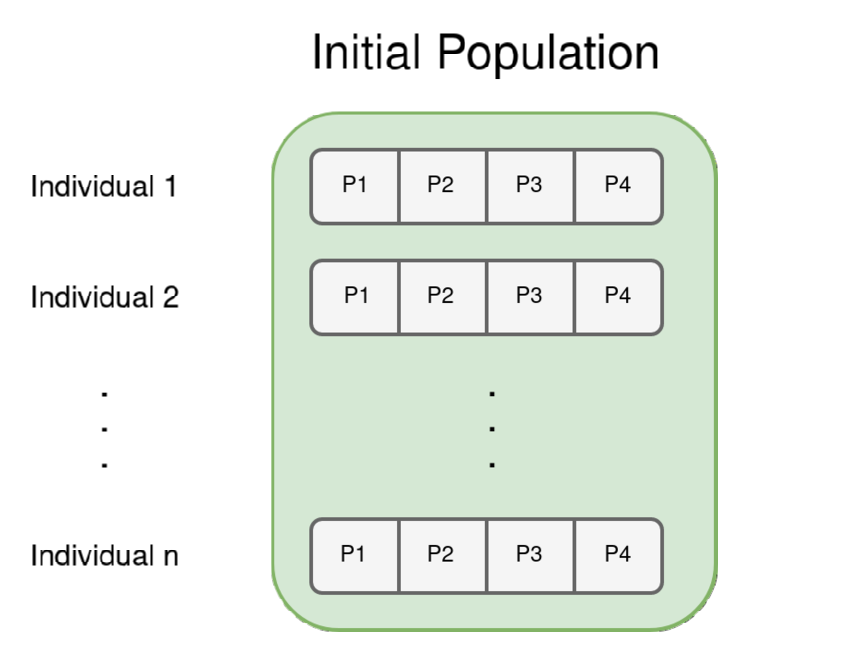
\includegraphics[width=6cm]{Figures/GA/inicializacion.png}
    \caption{TFM.}
    \label{GA_inicializacion}
\end{figure}
\begin{figure}[H]
    \centering
    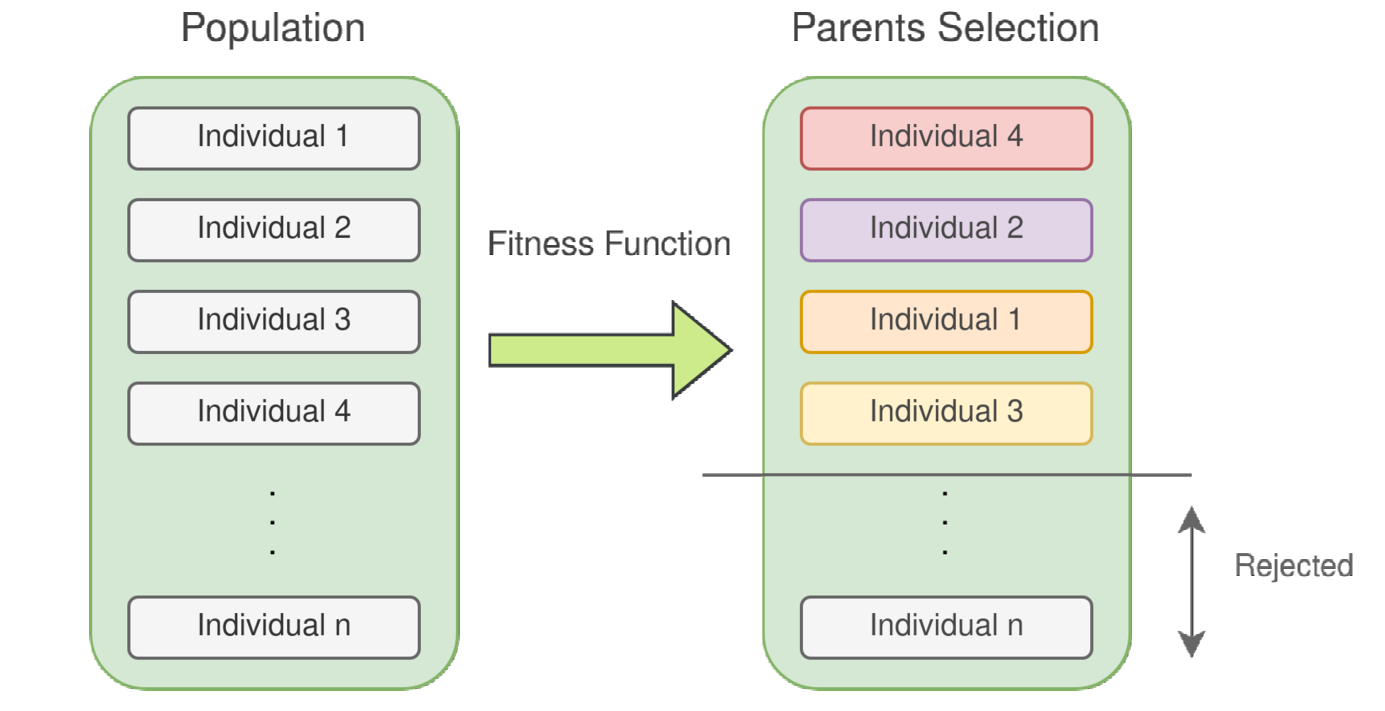
\includegraphics[width=8cm]{Figures/GA/selection.png}
    \caption{TFM.}
    \label{GA_selection}
\end{figure}
\begin{figure}[H]
    \centering
    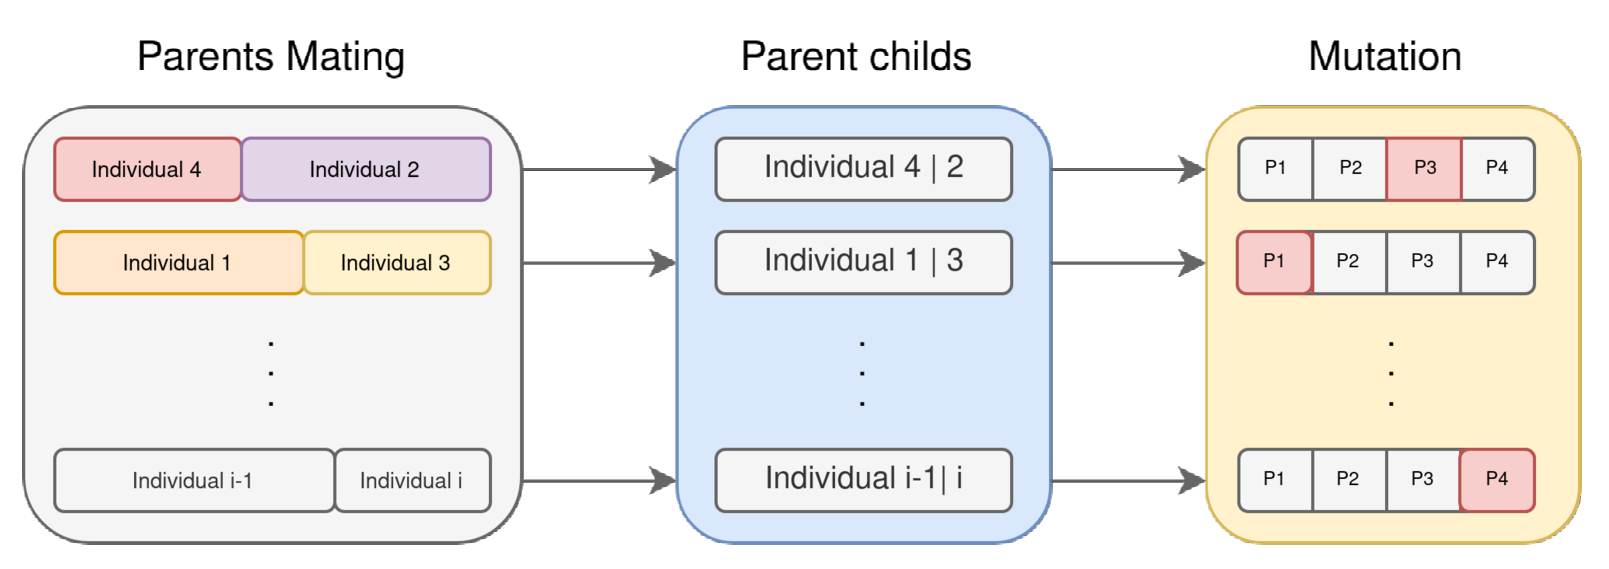
\includegraphics[width=10cm]{Figures/GA/cruce_mutacion.png}
    \caption{TFM.}
    \label{GA_cruce_mutacion}
\end{figure}

\section{Algoritmos de construcción de matrices}
\label{SOAT_MATRIX_ALGORITHM_CONSTRUCTION}

\textcolor{blue}{\textbf{Luis: hay que revisar la redacción, pero el enfoque propuesto es este.}}\\

La tendencia de utilizar modelos convolucionales a lo largo de la historia reciente ha tenido un notable incremento debido a la eficiencia y rendimiento que estos demuestran a lo largo de múltiples contextos. Estos modelos trabajan sobre datos matriciales bajo los que pueden aplicar convoluciones y encontrar patrones más o menos complejos sobre los que aprenden a clasificar las muestras. La naturaleza de los datos tabulares impide aplicar este tipo de modelos a este tipo de datos, ya  que no presentan una estructura matricial. Tanto es el incremento del uso de las convolucionales, que a lo largo de los últimos años se han diseñado técnicas para transformar datos tabulares a matriciales con el objetivo de poder aplicar estos modelos. Este problema no es un problema trivial, la forma en la que los datos son transformados a estas matrices debe generar una estructura que tenga sentido para los modelos convolucionales, maximizando la forma de representar laa información para estos modelos. 

En los últimos años se han diseñado distintas estrategias para solventar este problema, como OmicsMapNet \cite{ma2019omicsmapnet}, orientado a construir representaciones matriciales de las características de genes de pacientes que presentan cáncer. Para ello se consideran las descripciones bibliográficas de los genes para posicionar en localizaciones cercanas en la matriz aquellos que mayor semejanza presentan a través de Tree Map. Otro de los enfoques referentes en el estado del arte es DeepInsight \cite{Sharma2019}, que utiliza vectores de características de los datos originales para proyectarlos en un espacio bidimensional aplicando la visualización estadística T-SNE \cite{van2008visualizing}, donde aquellas características más cercanas bajo este espacio son seleccionadas para situarlas en posiciones cercanas de la matriz final construida. Más recientemente, se presentó REFINED (REpresentation of Features as Images with NEighborhood Dependencies) \cite{Bazgir2020}, una técnica que busca proyectar las características originales de los datos en un espacio bidimensional utilizando un escalador multidimensional bayesiano, que permite mantener la distribución de las características en su espacio dimensional original, posteriormente se aplica un algoritmo de Escalada Simple (hill climbing) que optimiza la asignación de las características a los píxeles finales de la imagen.

En lo que respecta a un de los enfoques más recientes en el estado del arte, se presenta Image Generator for Tabular Data (IGTD) \cite{Zhu2021}, una técnica que se aplica sobre descriptores de genes en pacientes que sufren cáncer. Esta técnica asigna las características más correlacionadas entre sí a posiciones cercanas dentro de la matriz, con el objetivo de aplicar una red neuronal convolucional que pueda operar sobre ella. Para lograr esto hace uso de técnicas de minimización de rankings entre pares de características y técnicas de minimización de rankings entre píxeles, donde en cada iteración se reasignan pares de características a la posición de aquellas otras que no han sido consideradas desde hace tiempo. De esta forma se logra una representación final de la matriz que resulta en agrupación de características similiares cercanas.


\section{Algoritmos de medición de importancia de características}
\label{SOAT_FEATURE_IMPORTANCE_METHODS}

\textcolor{blue}{\textbf{Luis: hay que revisar la redacción, pero el enfoque propuesto es este.}}\\


En el campo de la Inteligencia Artificial y Análisis de Datos la medición de la importancia de las características dentro de un conjunto de datos toma un papel clave para distintos propósitos. Estas técnicas permiten conocer el peso que tienen cada una de las variables respecto al resto de ellas para un conjunto de datos, ya sea por la relación que presentan entre sí (fácilmente deducible por el ser humano o no), o por la importancia que han tenido a la hora de construir un modelo predictivo. Comúnmente, valores más altos de importancia representan una mayor relevancia de una característica para...

En el estado del arte, existen distintos métodos que tienen como propósito medir el peso de las características en un conjunto de datos, tanto para problemas de regresión como de clasificación. Uno de los enfoques más clásicos dentro del Aprendizaje estadístico para problemas de naturaleza regresiva es la técnica de Regresión Lineal, donde la magnitud de las variables está basada en el valor y la dirección de los coeficientes en base al resultado del aprendizaje del método predictivo. Tomando como referencia esta base, existen enfoques más complejos derivados de esta técnica, como son las Elastic Net Regression, que durante el proceso de aprendizaje del modelo de Regresión Lineal, se utilizan términos de penalización para reducir los coeficientes del predictor. Por otra parte, existen técnicas orientadas exclusivamente a problemas de clasificación que permtien medir la importancia de las características. Un método muy común en este campo es la Regresión Logística, un modelo estadístico que tiene como objetivo deducir la probabilidad de que ocurra un evento binario en función de uno o más predictores. Para calcular la importancia de las características, se utilizan las probabilidades logarítmicas para un cambio de una unidad en la variable predictiva. Los valores absolutos más grandes indican una relación más fuerte entre el predictor y la variable objetivo \cite{Saarela2021}.

Permutation Feature Importance (https://academic.oup.com/bioinformatics/article/26/10/1340/193348?login=false)
Feature Selection with Importance: no he encontrado nada en 2 min.\\
Linear Regression Feature Importance: https://machinelearningmastery.com/calculate-feature-importance-with-python/

Por otra parte, existen otras técnicas que se alejan del aprendizaje estadístico y son métodos ampliamente utilizados para calcular la importancia de las variables, como los algoritmo de aprendizaje supervisado Random Forest. Estos métodos modelos cuyo funcionamiento se basa en la composición de varios modelos para dar una clasificación final (ensembles).

Dentro la filosofía de los modelos ensemble, los algoritmos Random Forest pertenecen a la tipología Bagging, que se basan en el concepto de crear múltiples modelos que son entrenados con distintas técnicas de reemplazo (boostrap) sobre los datos, y la predicción final del conjunto es la combinación de la salida de cada uno de ellos de manera independiente por votación. Este enfoque de los algoritmos ensemble permite obtener modelos robustos que son menos sensibles al sobreajuste de un modelo general. Random Forest se compone en N árboles de decisión, donde cada uno de ellos es entrenado con un subconjunto de muestras y características de forma independiente para dar lugar a un modelo combinado donde la predicción de nuevas muestras se elige aquella clase más votada de entre todo el conjunto de árboles. La importancia de las características en este algoritmo se calcula mediante el peso que ha tenido cada característica a la hora de construir los árboles, en función del número de muestras que divide en cada nivel.

No obstante, existe otra técnica más potente dentro de los ensembles que tiene como base el funcionamiento de los Random Forest, el algoritmo tipo Boosting XGBoost \cite{Chen_2016}. Los algoritmo tipo Boosting que se caracterizan por crear modelos secuencialmente donde cada nuevo modelo se enfoca en corregir los errores cometidos por los modelos anteriores. XGBoost construye N árboles de decisión secuenciales, donde cada uno de estos se centra en corregir el error cometido por el error anterior, reduciendo así el sesgo y mejorando la precisión del modelo final al enfocarse en reducir el error de los modelos anteriores. Esta técnica es ampliamente utilizada para problemas de XXXX \ref{BoostingExample} [1].

\begin{figure}[H]
    \centering
    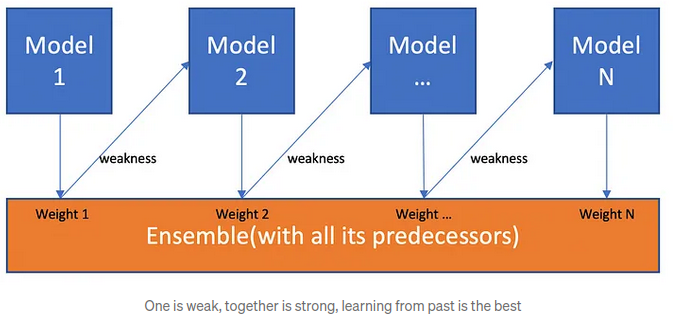
\includegraphics[width=14cm]{Figures/boosting_example.png}
    \caption{Alguna imagen así hecha por mi.}
    \label{BoostingExample}
\end{figure}

[1] (https://towardsdatascience.com/boosting-algorithms-explained-d38f56ef3f30)

[2] https://medium.com/geekculture/xgboost-versus-random-forest-898e42870f30


https://towardsdatascience.com/best-practice-to-calculate-and-interpret-model-feature-importance-14f0e11ee660

% \section{Algoritmos Boosting}

% \textbf{Luis: jornada de reflexión sin redactar.} Yo creo que es que no hay boosting algorithms que ofrezcan la importancia de las características, creo  que de los pocos es el XGBoost. Hay que cercinoarse. No obstante, he visto esto:
% https://pubs.acs.org/doi/full/10.1021/ci0500379


\section{Algoritmos CNN}

\underline{Explicación des diferentes algoritmos CNN con los que luego te comparas, con sus formulas y explicacion}

\textcolor{blue}{\textbf{Luis: hay que terminar y revisar la redacción, en la estructura me he liado, seguramente haya que reestructurarlo con el contenido que hay escrito.}}\\


Las redes neuronales convolucionales (CNNs) son modelos de Inteligencia Artificial supervisados que principalmente están orientados al reconocimiento de patrones en imágenes. Estos modelos han sido ampliamente utilizados para distintos objetivos, como clasificación de imágenes, detección de elementos de interés dentro de estas o problemas de regresión. La naturaleza de su arquitectura ha permitido que además, estos modelos sean aplicados al campo de la Inteligencia Artificial Generativa, como la creación d recommend thate nuevas imágenes mediante GAN, autoencoders o representación n-ndimensional de representaciones a través embeddings mediante el entrenamiento de redes siamesas, etc.

La principal característica que distingue a estos modelos respecto al resto de redes neuronales, y los hace especialmente efectivos en problemas basados en imágenes, es que su arquitectura se basa en capas convolucionales. Estas capas están compuestas por filtros, que durante el proceso de entrenamiento aprenden operaciones que se aplican sobre los datos de entrada, permitiendo así generar y reconocer patrones que se encuentren presentes en ellos.

Dentro de las redes neuronales convolucionales existen diferentes tipos, cada uno con sus ventajas y desventajas en funcón del problema que se quiere resolver. No obstante, existen partes comunes a ellas que es necesario mencionar, las capas de las que normalmente constan estas redes son las siguientes:

\begin{enumerate}
    \item \textbf{Capas Convolucionales:} Estas capas aplican convoluciones sobre las muestras de entrada. Las convoluciones no son más que multiplicaciones sobre posiciones de un vector que calculan la suma ponderada de todos los vecinos de la muestra de entrada para dar lugar a un único resultado en su salida, que será asignado a la salida de la capa convolucional en la misma posición sobre la que se ha aplicado la operación sobre la muestra de entrada. Los valores de ponderación (pesos) de esta suma son aprendidos por la red en su etapa de entrenamiento.
    
    \item \textbf{Filtros:} Los filtros son pequeñas matrices de las que están compuestas las capas convolucionales y son utilizadas para realizar las operaciones. Cada uno de estos filtros tiene asociado una serie de pesos en cada posición de la matriz. Estos filtros, al ser aplicados, generan los denominados feature maps, que no son más que mapas de activación sobre los que se aplicarán la función de activación.
    
    \item \textbf{Función de Activación:} activation functions in CNNs introduce non-linearities, enabling the network to learn complex patterns and relationships within the data, typically, an activation function like ReLU (Rectified Linear Unit) is applied element-wise to the feature maps to introduce non-linearity. \begin{center}
        $\text{ReLU}(x) = \max(0, x)$
    \end{center}
    
    \item \textbf{Capas Pooling:} estas capas aplican operaciones sobre los mapas de características con el objetivo de simplificar la información y reducir la dimensionalidad, que permite reducir la complejidad computacional de las redes durante su entrenamiento. Estas operaciones tienen una naturaleza de agrupación que son aplicadas en pequeñas zonas de los mapas de características para simplificar áreas y contemplar patrones relevantes en ellas. Estas operaciones pueden ser promediar un conjunto de características, mantener el mínimo de ellas o el máximo entre otras.
    
    \item \textbf{Capas Densas:} Las capas densas son capas que interconectan completamente un conjunto de entrada de neuronas con las neuronas especificadas en esta capa. A diferencia de su aplicación en otro tipo de redes neuronales, en las redes convolucionales estas capas toman como entrada el conjunto de características extraídas de los procesos convolucionales para dar lugar a una clasificación final.
    \begin{center}
        $z_i = \sum_{j=1}^{n} w_{ij} \cdot x_j + b_i$\\
        $y_i = f(z_i)$
    \end{center}
\end{enumerate}

\underline{CNN-1D}

Las redes neuronales convolucionales unidimensionales (CNN-1D) son redes cuya característica principal es que los filtros que aplican en cada una de sus convoluciones son de una dimensión \cite{CNN1D}.

$$(f * g)[n] = \sum_{m=0}^{M-1} f[m] \cdot g[n-m]$$

Estos modelos son ampliamente utilizados para problemas orientados a detecciones de patrones en señales, donde la naturaleza de los datos es principalmente secuencial. Por ejemplo, algunas de las aplicaciones donde las CNN-1D han demostrado ser efectivas han sido el monitoreo de electrocardiograma en tiempo real \cite{Kiranyaz2017tt}, detección de daños estructurales basada en vibraciones en infraestructuras civiles \cite{khodabandehlou2019vibration} o para clasifiación de audios musicales \cite{allamy20211d}. Estas arquitecturas son una buena opción en problemas de este tipo, tanto en la calidad de resultados que presentan en este dominio, como en la rapidez de inferencia que demuestran, permitiendo ser aplicadas en tiempo real en dispositivos que requieren baja demanda de recursos computacionales, como teléfonos móviles. Sin embargo, la principal limitación de estas arquitecturas se 

\underline{CNN-2D}


El proceso de aprendizaje de las redes neuronales está dividido en varias fases. Las redes en su etapa de entrenamiento realizan predicciones sobre los datos de entrada, aplicando operaciones matemáticas sobre ellos utilizando los pesos configurados en la red (Forward Propagation).

\textbf{Forward Pass:}
\[ Z = W \cdot X + b \]
\[ A = \sigma(Z) \]


Posteriormente, en la capa clasificadora, los valores predichos son comparados con el valor real de las muestras que han sido introducidas en esta etapa a la red, de tal forma que el error que han producido sobre estas muestras durante esta fase es medible y calculado mediante una función de pérdida.

\textbf{Loss Calculation:}
\[ \text{Loss} = \text{Calculate Loss}(\text{Actual}, \text{Predicted}) \]

Gracias a la derivabilidad de las funciones que componen la red, en función de este error los pesos asociados a cada una de las capas de la red son optimizados con el objetivo de minimizar el error en la siguiente etapa de entrenamiento (Back Propagation). Gracias a la repetición de estos procesos la red la red toma conocimiento sobre los datos.

\textbf{Backward Pass (Calculating Gradients):}
\[ \frac{\partial \text{Loss}}{\partial Z} = \frac{\partial \text{Loss}}{\partial A} \times \frac{\partial A}{\partial Z} \]
\[ \frac{\partial \text{Loss}}{\partial W} = \frac{\partial \text{Loss}}{\partial Z} \cdot X^T \]
\[ \frac{\partial \text{Loss}}{\partial b} = \text{sum of} \, \frac{\partial \text{Loss}}{\partial Z} \, \text{over the examples} \]

\textbf{Updating Weights and Biases:}
\[ W = W - \alpha \cdot \frac{\partial \text{Loss}}{\partial W} \]
\[ b = b - \alpha \cdot \frac{\partial \text{Loss}}{\partial b} \]

Para llevar a cabo este proceso, es necesario especificar la función de pérdida que medirá el error durante la fase de entrenamiento. La función de pérdida más común en problemas de clasificación binaria es la Binary Cross Entropy:

$$\text{Binary Cross Entropy} = \frac{-1}{N} \sum_{i=1}^{N} (y_{i}*\log{p_{i}}+ (1 - y_{i})*\log{(1-p_{i}})).$$

Donde:

\begin{itemize}
    \item $N$ es el número de muestras totales en el conjunto de datos.
    \item $y_i$ es la etiqueta de la clase (0 ó 1) de la muestra actual.
    \item $p_i$ es la probabilidad de que la muestra actual pertenezca a la clase 1.
    \item log⁡log denotes the natural logarithm.
\end{itemize}

Esta ecuación penaliza en tiempo de entrenamiento la clasificación errónea de las muestras. El término $(y_{i}*\log{p_{i})$ penaliza la probabilidad $p_i$ de pertenencia de la muestra $y_i$ a la clase 0, siempre y cuando el valor verdadero de la muestra sea la clase 1. Por el contrario, el término $y_{i}*\log{p_{i}}+ (1 - y_{i})*\log{(1-p_{i}})$ penaliza la probabilidad $p_i$ de la muestra $y_i$ de pertenencia a la clase 1 siempre y cuando el valor real sea la clase 0. Valores de probabilidad altos $p_i$ de la predicción de la red a las clases incorrectas, generan una acumulación del error.  El símbolo negativo de la ecuación describe la minimización de esta función de pérdida. Esta función se utilizará para actualizar los pesos de toda la red mediante Back Propagation de cara a minimizar esta función para la siguiente época.

Una vez se define la función de pérdida de la red, la actualización de los pesos internos de las capas de la red y por tanto, el conocimiento de la misma sobre los datos, viene dado por el proceso de Back Propagation. Este proceso hace uso de la regla de la cadena, que permite calcular las derivadas parciales de la función de pérdida con respecto a los pesos de la red neuronal. Esto se aplica mediante el cálculo de las derivadas parciales de las capas superiores para calcular las derivadas de las capas inferiores. Comienza a partir de la capa de salida, retrocediando a través de las capas ocultas, actualizando los pesos de la red conjuntamente en cada etapa.



\section{Modelos estado del arte}
\underline{Modelos del estado del arte contra los que nos comparamos.}\\
\textcolor{blue}{\textbf{Luis: esto lo he metido yo. Según tengo entendido tenemos que poner fórmulas de todos los modelos, incluyendo los 5 ó 6 contra los que nos comparamos no? Simplemente he copiado las fórmulas de ChatGPT}}\\

Estadísticos

\underline{Naive Bayes}
\[
P(C_k | x_1, x_2, \ldots, x_n) = \frac{P(C_k) \cdot P(x_1, x_2, \ldots, x_n | C_k)}{P(x_1, x_2, \ldots, x_n)}
\]

Where:
\begin{itemize}
    \item $P(C_k | x_1, x_2, \ldots, x_n)$ is the posterior probability of class $C_k$ given the features.
    \item $P(C_k)$ is the prior probability of class $C_k$.
    \item $P(x_1, x_2, \ldots, x_n | C_k)$ is the likelihood, the probability of observing the given features given class $C_k$.
    \item $P(x_1, x_2, \ldots, x_n)$ is the probability of observing the features.
\end{itemize}


\underline{Logistic Regression}

Logistic Regression models the probability $P(Y = 1|X)$ of a binary outcome $Y$ given predictors $X = (X_1, X_2, \ldots, X_n)$ using the logistic function:

\[
P(Y = 1|X) = \frac{1}{1 + e^{-(\beta_0 + \beta_1 X_1 + \beta_2 X_2 + \ldots + \beta_n X_n)}}
\]

Where:
\begin{itemize}
    \item $P(Y = 1|X)$ is the probability of the positive class given the predictors.
    \item $\beta_0, \beta_1, \beta_2, \ldots, \beta_n$ are the coefficients.
    \item $X_1, X_2, \ldots, X_n$ are the predictor variables.
    \item $e$ is the base of the natural logarithm.
\end{itemize}

No supervisados

\underline{KNN}
The k-Nearest Neighbors (KNN) algorithm predicts the class of a data point by considering its $k$ nearest neighbors in the feature space. The predicted class $\hat{y}$ for a new data point $x$ is determined by a majority vote among its $k$ nearest neighbors:

\[
\hat{y} = \arg\max_{y_i} \sum_{i=1}^{k} I(y_i = y)
\]

Where:
\begin{itemize}
    \item $\hat{y}$ is the predicted class for the new data point.
    \item $x$ is the new data point to be classified.
    \item $k$ is the number of nearest neighbors to consider.
    \item $y_i$ represents the classes of the $k$ nearest neighbors.
    \item $I(y_i = y)$ is an indicator function returning 1 if $y_i$ is equal to the predicted class $y$, and 0 otherwise.
\end{itemize}

Supervisados

NNs

\underline{MLP}

A Multi-Layer Perceptron (MLP) is a type of feedforward neural network composed of multiple layers, including an input layer, hidden layers, and an output layer. Let's denote:

\begin{itemize}
    \item $x = (x_1, x_2, \ldots, x_n)$ as the input vector.
    \item $h^{(i)} = (h_1^{(i)}, h_2^{(i)}, \ldots, h_{m_i}^{(i)})$ as the activations of the $i$-th hidden layer.
    \item $W^{(i)}$ as the weight matrix connecting the $i$-th and $(i+1)$-th layers.
    \item $b^{(i)}$ as the bias vector added to the $i$-th layer.
    \item $f$ as the activation function.
    \item $y = (y_1, y_2, \ldots, y_k)$ as the output vector.
\end{itemize}

The computation in an MLP can be represented as follows:

\[
h^{(i)} = f(W^{(i)}h^{(i-1)} + b^{(i)})
\]

where $h^{(i-1)}$ is the activation from the previous layer.

The final output of the MLP is computed as:

\[
y = f(W^{(n)}h^{(n-1)} + b^{(n)})
\]

Here, $n$ represents the number of hidden layers in the MLP.

\underline{Random Forest}

\begin{enumerate}
    \item For $t = 1$ to $T$ (the number of trees in the forest):
        \begin{enumerate}
            \item Draw a bootstrap sample $D_t$ by sampling with replacement from $D$.
            \item Grow a decision tree $T_t$ using $D_t$:
                \begin{itemize}
                    \item For each node of the tree:
                        \begin{enumerate}
                            \item Randomly select $m$ features from $M$.
                            \item Split the node using the best feature among the $m$ selected features.
                        \end{enumerate}
                \end{itemize}
        \end{enumerate}
    \item The final prediction for a new sample is obtained by aggregating predictions from all trees (for classification, typically a majority vote).
\end{enumerate}


\underline{SVC}

The Support Vector Classifier (SVC) aims to find the optimal hyperplane that best separates data into different classes. Given a training dataset $\{(x_i, y_i)\}$ where $x_i \in \mathbb{R}^n$ represents input features and $y_i \in \{-1, 1\}$ represents class labels, the objective of the SVC is to find:

\[
\min_{w, b, \xi} \frac{1}{2} ||w||^2 + C \sum_{i=1}^{m} \xi_i
\]

subject to:

\[
y_i(w \cdot x_i + b) \geq 1 - \xi_i, \quad \xi_i \geq 0
\]

Where:
\begin{itemize}
    \item $w$ is the weight vector of the hyperplane.
    \item $b$ is the bias term.
    \item $\xi_i$ are slack variables allowing for misclassification or data points within the margin.
    \item $C$ is a regularization parameter controlling the trade-off between maximizing the margin and minimizing the classification error.
\end{itemize}

The decision function for classifying a new sample $x_{\text{new}}$ is given by:

\[
\text{Predict}(x_{\text{new}}) = \text{sign}(w \cdot x_{\text{new}} + b)
\]

\underline{LSTM para \cite{app7060476}}
LSTM Equations:

\begin{align*}
i_t &= \sigma(W_{xi}x_t + W_{hi}h_{t-1} + W_{ci}c_{t-1} + b_i) \\
f_t &= \sigma(W_{xf}x_t + W_{hf}h_{t-1} + W_{cf}c_{t-1} + b_f) \\
g_t &= \text{tanh}(W_{xg}x_t + W_{hg}h_{t-1} + b_g) \\
o_t &= \sigma(W_{xo}x_t + W_{ho}h_{t-1} + W_{co}c_{t} + b_o) \\
c_t &= f_t \odot c_{t-1} + i_t \odot g_t \\
h_t &= o_t \odot \text{tanh}(c_t)
\end{align*}
}


\section{Medidas de evaluación de una red neuronal}
\underline{Aquí explicas el F1-score y demás, con sus fórmulas y con detalle.}

\textcolor{blue}{\textbf{Luis: esto yo creo que estaría OK.}}\\

En este apartado se presentan los indicadores de calidad utilizados para medir el rendimiento y generalización de los modelos expuestos en esta tesis. Uno de los componentes fundamentales en el desarrollo de modelos de Inteligencia Artificial es conocer la capacidad y calidad de los modelos ante la predicción de nuevas muestras que nunca ha visto durante su etapa de entrenamiento, tanto como para poder compararlos como para conocer en profundidad cómo se comportan los modelos ante nuevas situaciones.

Para evaluar los modelos, es común aplicar una fase de validación o de test, donde se utilizan los modelos para realizar predicciones contra muestras de las que se conoce su variable verdadera. De esta forma es posible comparar la calidad de los modelos respecto a muestras que nunca antes han visto y aplicar fórmulas y métricas que nos dan idea del rendimiento de los modelos. Para esto, es necesario introducir dos conceptos básicos TP, FP, FN y TN, estos datos son calculados para cada una de las clases que puede predecir el modelo.

\begin{enumerate}
    \item \textbf{True Positives:} Los True Positives (TP) representan el número de muestras que han sido correctamente clasificadas por el modelo como positivas. Es decir, el modelo clasifica correctamente la muestra como la clase a la que pertenece.
    \item \textbf{True Negatives:} Los True Negatives (TN) representan el número de muestras que han sido correctamente clasificadas por el modelo como negativas. Es decir, el modelo
    \item \textbf{False Positives:} Los False Positives (FP) representan el número de muestras que han sido incorrectamente clasificadas por el modelo como positivas. Es decir, el modelo ha clasificado una muestra que no pertenecía a esa clase como positiva.
    \item \textbf{False Negatives:} Los False Negatives (FN) representan el número de muestras que han sido incorrectamente clasificadas por el modelo como negativas. Es decir, el modelo ha clasificado una muestra positiva como negativa.
\end{enumerate}

En función del problema que nos encontremos, es posible que sea preferible un modelo que tienda a más a un tipo de clasificación que a otra debido a la criticidad del problema a costa de reducir el número de ocurrencias de otro indicador. No tiene la misma importancia matar a cinco personas por FN que darle un medicamento a 5 que realmente no la necesitan (FP) pero que no sufrirían de consecuencias graves al tomarlo. Es por ello que utilizando estos conceptos básicos es posible crear indicadores de calidad que ofrezcan más información para cada una de las clases predichas. En el estado del arte, se utilizan dos métricas comunes que pueden ser utilizadas para la composición de indicadores aún más complejos, estas métricas son calculadas para cada una de las posibles clases dentro del conjunto de datos.

La primera de ellas es la precisión (Precision), que mide el porcentaje de muestras clasificadas correctamente de una clase, respecto al total de muestras que existen de dicha clase en el conjunto de datos.

$$\text{Precision} = \frac{{\text{True Positives}}}{{\text{True Positives} + \text{False Positives}}}$$

Por otra parte, el Recall representa la proporción de elementos de una clase que el modelo identifica correctamente como esa clase.

$$\text{Recall} = \frac{{\text{True Positives}}}{{\text{True Positives} + \text{False Negatives}}}$$

Existe otra métrica que combina los dos indicadores anteriores, considerando la precisión que tiene el modelo a la hora de predecir muestras como una clase y cuántos de los casos positivos fueron captados por el modelo (recuerdo), de tal forma que para cada cada una de las clases se pueda obtener una evaluación individual, siendo más sencillo en análisis sobre esto. 

$$\text{F1 score} = 2 \times \frac{{\text{precision} \times \text{recall}}}{{\text{precision} + \text{recall}}}$$

\chapter{Construcción de un modelo de predicción de la gravedad de un accidente de tráfico}

\textcolor{blue}{\textbf{Luis: esta intro y todo el punto del modelo preeliminar no me termina de convencer, lo hablamos cuando podais.}}\\


En esta tesis se expone una metodología y un modelo general de predicción de gravedad de accidentes de tráfico aplicable a cualquier región. Para llegar a este fin, inicialmente se realizó una investigación y se implementó una primera metodología a modo de propotipo sobre la que aplicar modificaciones hasta llegar al objetivo final, un procedimiento que no fuese sensible a la disponibilidad de datos y fuera independiente de la región sobre la que se aplicase, es decir, un modelo de predicción de la necesidad de asistencia en los accidentes de tráfico general. Por este motivo, este apartado se divide en dos subsecciones. La primera de ella describe la intuición sobre el primer prototipo, describiendo brevemente las fases que lo componen, los objetivos finales de este, incidiendo en las partes que han evolucionado respecto al modelo final. La siguiente sección de este apartado expone la metodología final tras la evolución del prototipo como referencia, justificando las decisiones tomadas en cada caso.

\section{Modelo preliminar}

\underline{Explicas el enfoque de paper 1, brevemente, a nivel metodológico.}\\
\textcolor{red}{Luis: a lo mejor estaría bien meter todo lo del congreso}\\

Este primer prototipo se presentó en el artículo \cite{PEREZSALA2023113245}, se implementó con el objetivo de predecir la gravedad de los accidentes de tráfico en la ciudad de Madrid, concretamente en tres clases distintas disponibles en este conjunto de datos: (1) Leves, (2) Severos y (3) Fatales.

Para llegar al entrenamiento de un modelo predictivo, se diseñó una metodología prototipo que estaba compuesta por cinco fases secuenciales \ref{figDegree}. Y tenía como objetivo  realizar transformaciones y operaciones sobre datos, inicialmente tabulares, para transformarlos en datos matriciales. De esta forma era posible experimentar con dos modelos convolucionales, el primero de ellos unidimensional y el segundo bidimensional, CNN-1D y CNN-2D respectivamente.

Para ello, era necesario definir una categorización de características, las cuales serían utilizadas como apoyo para la construcción de estas matrices que junto a la importancia de cada variable dentro del conjunto de datos, era posible asignarlas a coordenadas dentro de una matriz.

Finalmente la metodología y los modelos convolucionales propuestos eran comparados con otros tres modelos del estado del arte (GNB, SVC y KNN) para evaluar sus rendimientos respecto a la ciudad de Madrid.

A continuación se enumeran las etapas que definen el flujo de la metodología prototipo.

\begin{figure}[H]
    \centering
    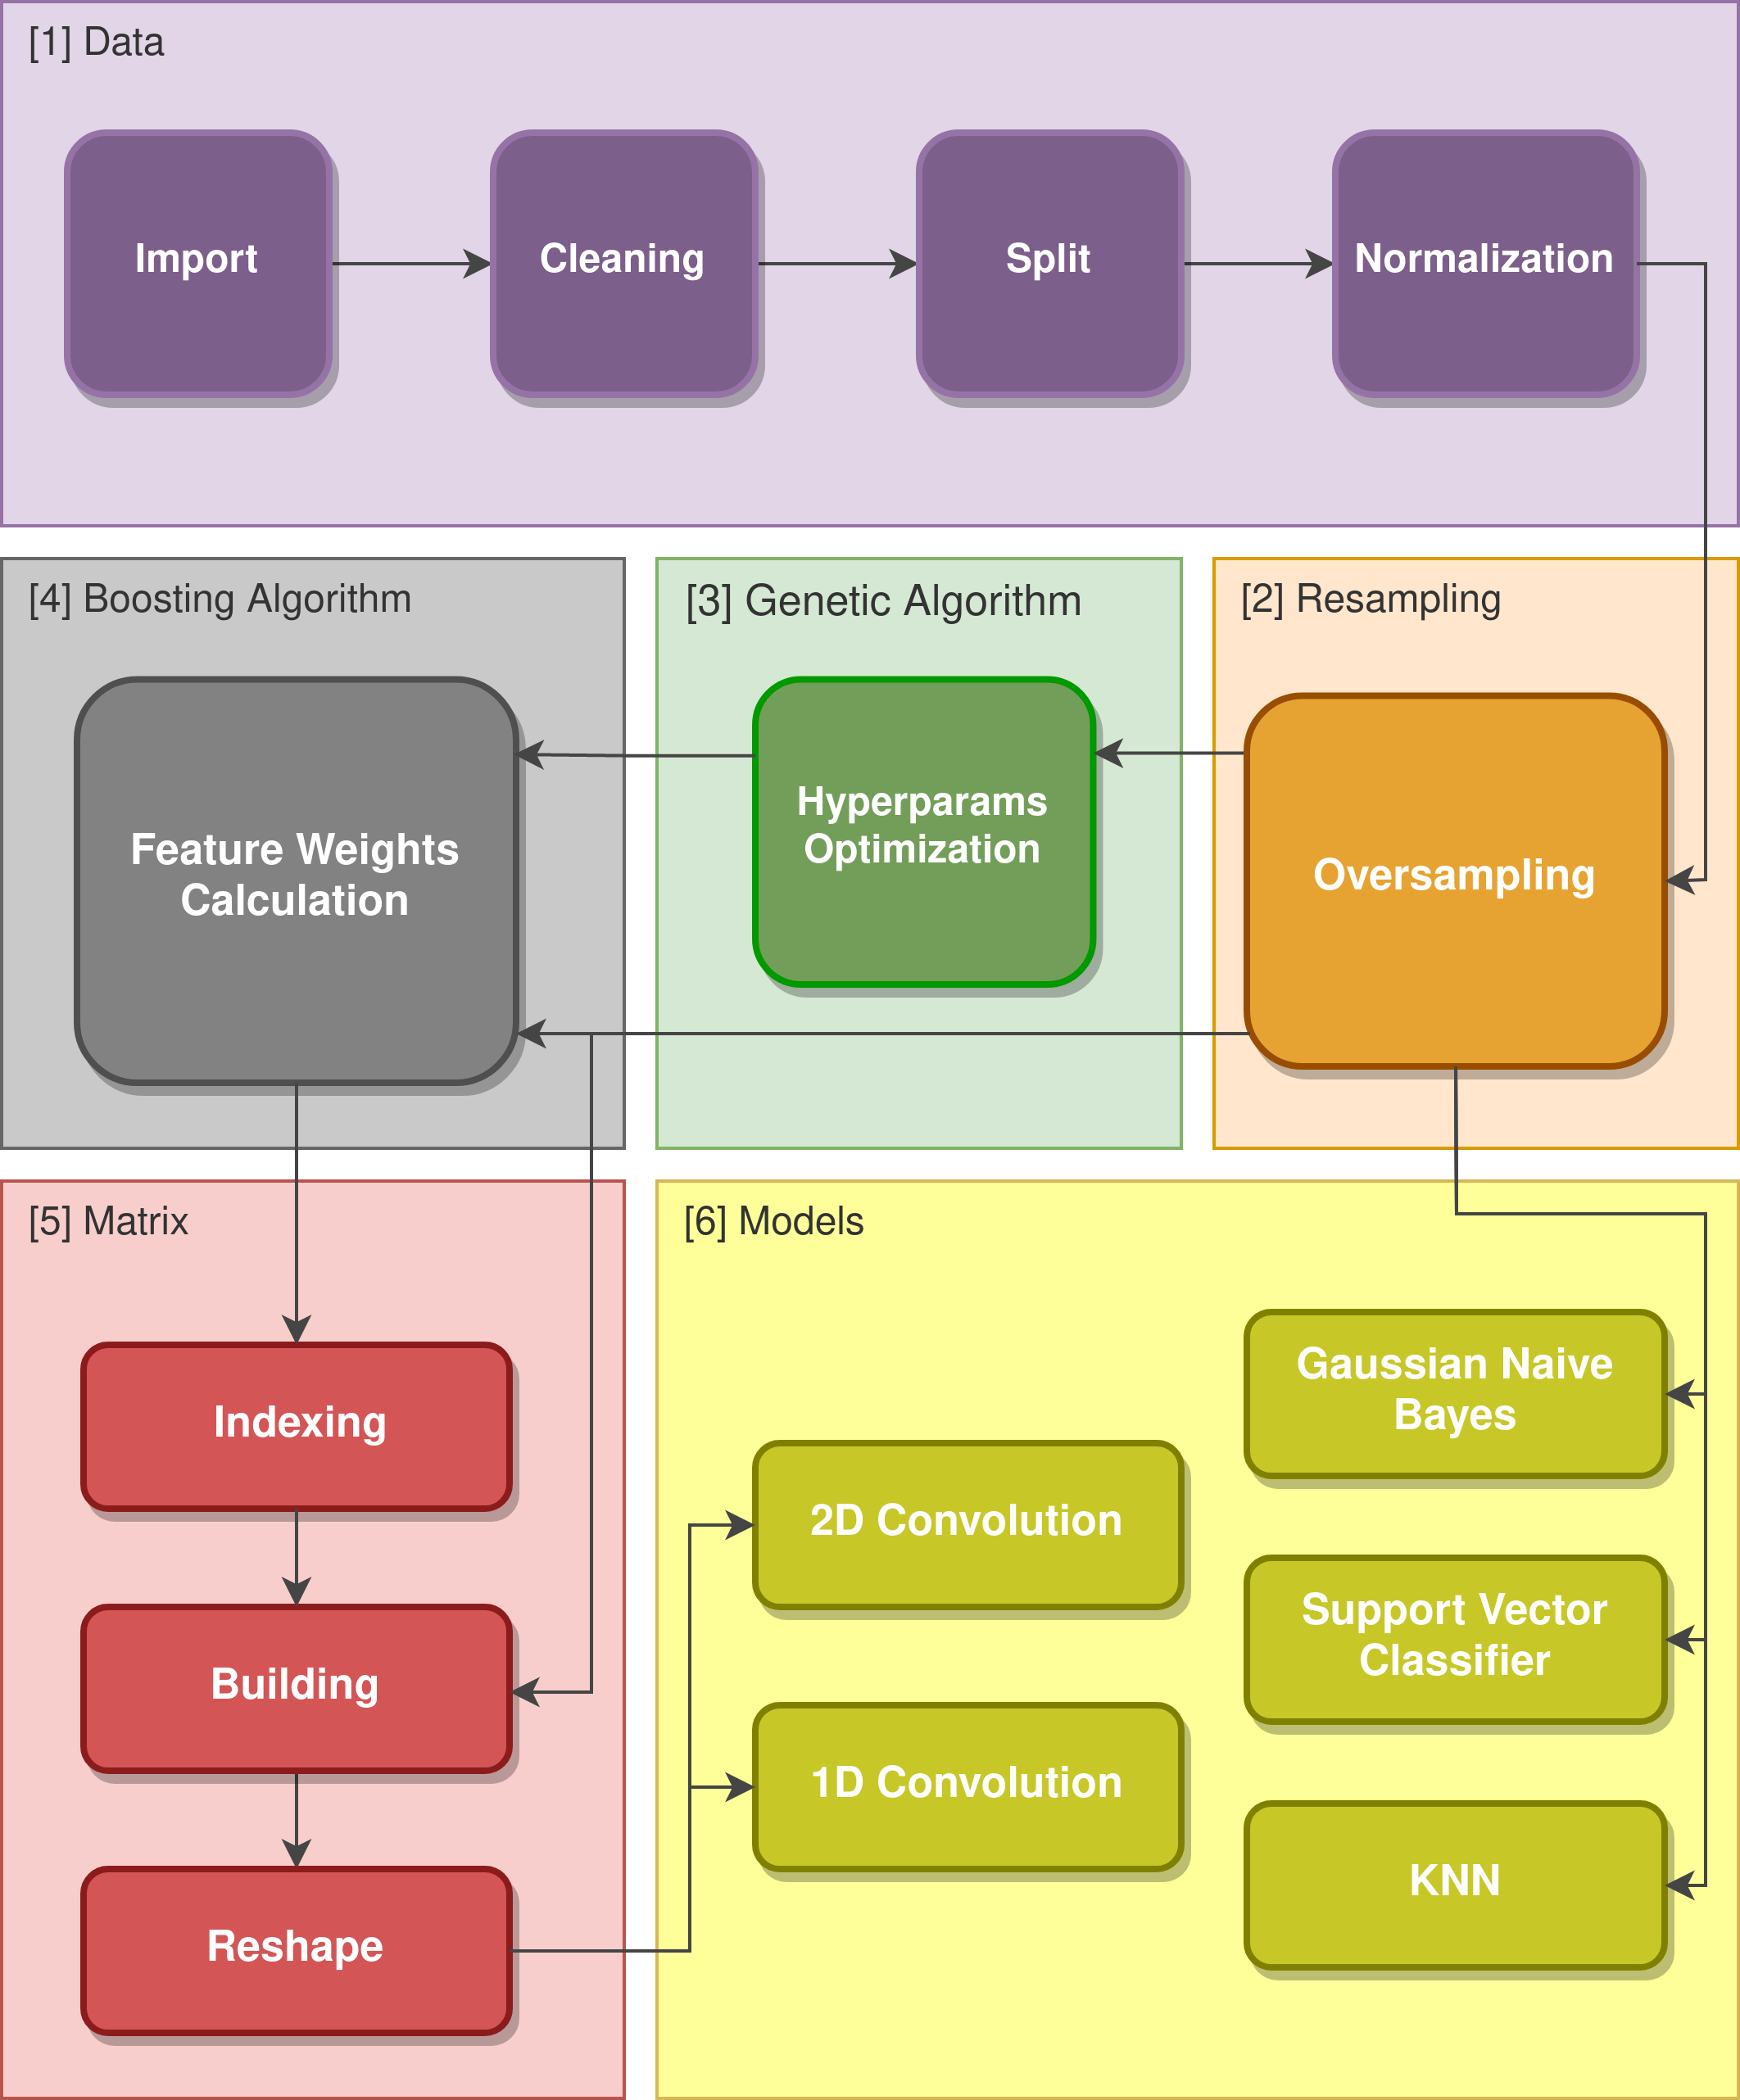
\includegraphics[width=3.5in]{Figures/1stPaper/Data_flow.png}
    \caption{Flow chart of the proposed model with its different phases.}
    \label{figDegree}
\end{figure}


\underline{[1] Datos}\\
La primera fase de esta metodología prototipo está orientada al tratamiento de los datos. Estos datos originales del dataset eran datos en bruto, donde se podían encontrar errores en los valores, valores atípicos y variables con valores cualitativos que había que discretizar. En esta etapa a los datos se les aplica un proceso de limpieza, discretización y normalización. Con el objetivo de construir un conjunto de datos interpretable por los modelos de Inteligencia Artificial.


\underline{[2] Resampling}\\
La segunda fase tenía como objetivo trabajar sobre el desbalanceo de los datos presente el dataset. Debido a la naturaleza de los accidentes de tráfico, gran parte de ellos eran de tipo leve, mientras que el resto de tipos de accidentes (severos y fatales), presentaban una proporción mucho menor respecto a los del primer tipo. Para evitar un sesgo en los modelos, y que tendiesen a predecir cualquier nueva muestra como la clase mayoritaria, se estudiaron distintas técnicas de balanceo de datos, utilizando finalmente la técnica Borderline SMOTE-II para balancear las clases minoritarias, aplicando generación de datos sintéticos hasta igualar las clases hasta la mayoritaria.

\textcolor{red}{\textbf{Luis:} Capaz que juntaba los algoritmos genéticos y el Boosting , es necesario saber del Boosting para justificar el uso de algoritmos genéticos}\\

\underline{[3-4] Algoritmos Genéticos / Boosting}\\
Para transformar los datos tabulares a datos matriciales interpretables por el modelo convolucional de dos dimensiones, se requería de algún tipo de estrategia para la asignación de cada una de las variables del dataset a coordenadas dentro de una matriz bidimensional, con el objetivo de aplicar los modelos convolucionales propuestos en este prototipo. Para llevar a cabo esto, se tomó una estrategia que requería de conocer la importancia de cada variable dentro del conjunto de datos. Como método para hallar el peso de cada característica dentro del dataset se utilizó un algoritmo tipo Boosting. Los algoritmos tipo boosting son un algoritmos clasificadores que ofrecen la importancia numérica de cada variable en función del peso que han tenido durante su entrenamiento. Estos algoritmos necesitan una configuración de hiperparámetros que se realizó mediante la evolución de un algoritmo genético.

\underline{[5] Matrices}\\
Una vez se disponían de los pesos de las características gracias al cálculo del algoritmo tipo Boosting, se categorizaron las variables en distintas características. Para tener una referencia de dos dimensiones sobre las que comenzar a indexar las variables. En primer lugar se calculó el peso total de las categorías, que era la suma de cada una de las características que contenía, como resultado de esto, cada categoría se indexaba a una fila de la matriz, donde aquella que más peso presentaba era asignada a la fila central, la segunda en la posición inmediatamente superior, la siguiente en la inferior y así sucesivamente. Las características que las componían se asociaban a las columnas dentro de su categoría de la misma manera, la de mayor peso en la posición central, la siguiente en su posición inmediatamente a la izquierda, la siguiente a la derecha etc. Como resultado de este proceso, cada registro perteneciente al dataset original era transformado en una matriz de 5x5.

\underline{[6] Modelos CNN propuestos}

Las arquitecturas prototipo propuestas constaban de cuatro capas convolucionales con tamaños de kernels de $1 \times 3$ para la CNN 1D y $3 \times 3$ para la CNN-2D respectivamente. Estos núcleos se proyectaban en $256$ y $512$ canales para formar el filtro convolucional asociado con cada capa. Porteriomente se aplicaba un proceso de normalización de batch a la salida de cada uno de los mapas de características.

El padding de los kernels estableció en $1$ para ambos tipos de redes, de modo que las convoluciones se apliquen agregando ceros a los límites de las matrices, y las sa $1$ para la CNN 1D y ${1, 1}$ para la CNN 2D. Por lo tanto, el desplazamiento de los núcleos se realiza píxel por píxel en ambas redes convolucionales.

En la salida de cada capa convolucional, se aplica la función de activación Unidad Lineal Rectificada (ReLU).

La salida de la última capa de convolución transforma la matriz de mapa de características generada de tamaño $5 \times 5$ en una capa que aplanará la matriz a un vector unidimensional de $1 \times 25$. A continuación, se aplica una capa densa que conecta cada uno de los $25$ nodos de la capa aplanada con los $128$ nodos de la capa densa, que genera los logits antes de aplicar la última función de activación Softmax que devuelve la clase predicha. En la figura \ref{TASPCNNIMAGE} se observa el diseño de la arquitectura de la red propuesta.

\begin{figure}[H]
	\centering
	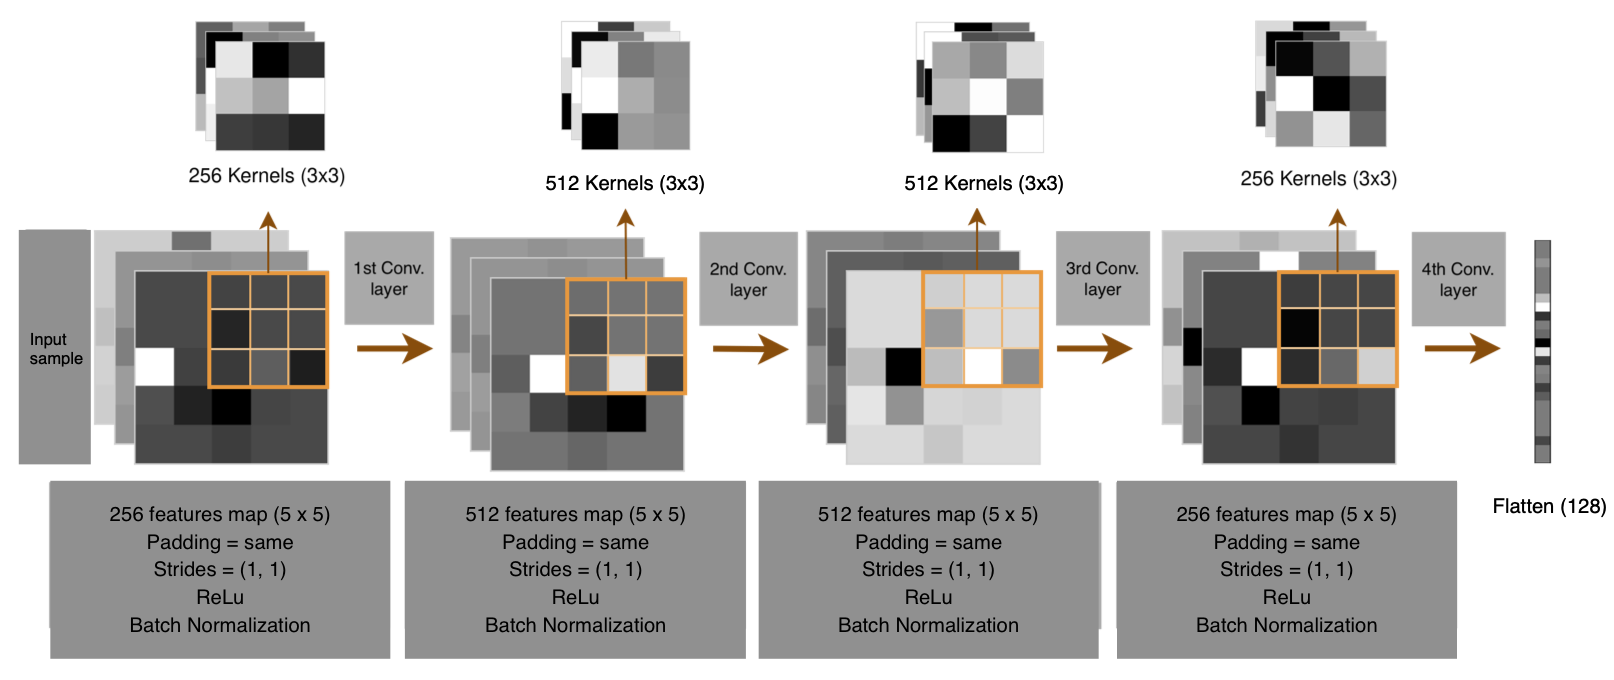
\includegraphics[width=16cm]{Figures/1stPaper/TASPCNN.png}
	\caption{Architecture of the 2D-Convolutional neural network.}
	\label{TASPCNNIMAGE}
\end{figure}

\underline{[7] Comparaciones}\\
Por último se compararon los dos modelos propuestos (CNN-1D y CNN-2D) contra 3 modelos del estado del arte.


\underline{Conclusiones..}
Analizando los resultados de la metodología y modelo prototipo se observa que la decisión de dividir los accidentes de tráfico en tres clases, ofrece una utilidad bastante pobre. Siendo dos de estas clases minoritarias y aplicando generaciónn de datos sintéticos contra tantas muestras de accidentes leves podría carecer de sentido a nivel práctico.
El siguiente paso para resolver esto fue la categorización de estos accidentes en dos clases, además de implementar un proceso de filtrado de áreas que uscaba rebajar el número de accidentes tipo leve de forma natural en el conjunto de datos.
Otra de las propuestas de mejora y que tenía todo el sentido del mundo era incrementar el número de características. A medida que se dispone de mayor información en el conjunto de datos

\section{Modelo GTAAF}
Después de analizar los resultados ofrecidos del primer prototipo, encontrar debilidades en los enfoques y decisiones tomadas, se propone una nueva metodología basada en la anterior. Esta nueva metodología denominada GTAAF (General Model for Traffic Accident Assistance Forecasting), busca incrementar el rendimiento de su predecesora, con el principal objetivo de diseñar un procedimiento de predicción de asistencia de accidentes generalizable a cualquier región. El principal problema de los conjuntos de datos de accidentes es que dependiendo de la región y/o gobierno que los ofrezca, estos disponen de información muy dispar entre ellos, debido principalmente al coste que supone obtener ciertos datos y/o la naturaleza social de la población. Ss por esto que en caso de querer aplicar un modelo de predicción de necesidad de asistencia en accidentes, requiere un trabajo de analizar qué categorías están disponibles y cuáles pueden ser influyentes en la necesidad de asistencia de los accidentes. Para solventar esto y conseguir una generalización independiente de los datos disponibles, la metodología GTAAF propuesta se basa en categorización de las características disponibles individuales dependientes de cada conjunto de datos, donde en función de la naturaleza a la que pertenezca cada dato disponible estos puedan ser asignados a una de las categorías propuestas en esta metodología, cuyas propiedades son de fácil adquisición. Esto sortea las peculiaridades individuales de la disponibilidad de datos de cualquier región. Para evaluar esto, GTAAF es comparado con otros seis modelos del estado del arte a lo largo de 8 regiones distintas en las mismas condiciones.

En esta sección se explicará con detalle cada una de las etapas por las que pasan los datos, la justificación de las decisiones tomadas para la construcción de esta metodología y las principales diferencias entre la versión preliminar y la versión final.

En primer lugar, las fases de la nueva metodología son asignadas a tres etapas claramente diferenciadas: (1) la fase de Preprocesamiento, donde se contemplan procesos de limpieza de datos, transformación y balanceo de datos, (2) la fase de Postprocesado donde se aplican técnicas de transformación para representar los datos de accidentes en formato tabular a formato matricial, y (3) la fase de entrenamiento, donde se entrenará un modelo neuronal convolucional en base a esta representación para predecir la necesidad de asistencia en los accidentes. En la figura \ref{DataFlow} se muestran, en modo de diagrama, cada una de las fases que componen la metodología GTAAF.

\begin{figure}[H]
    \centering
    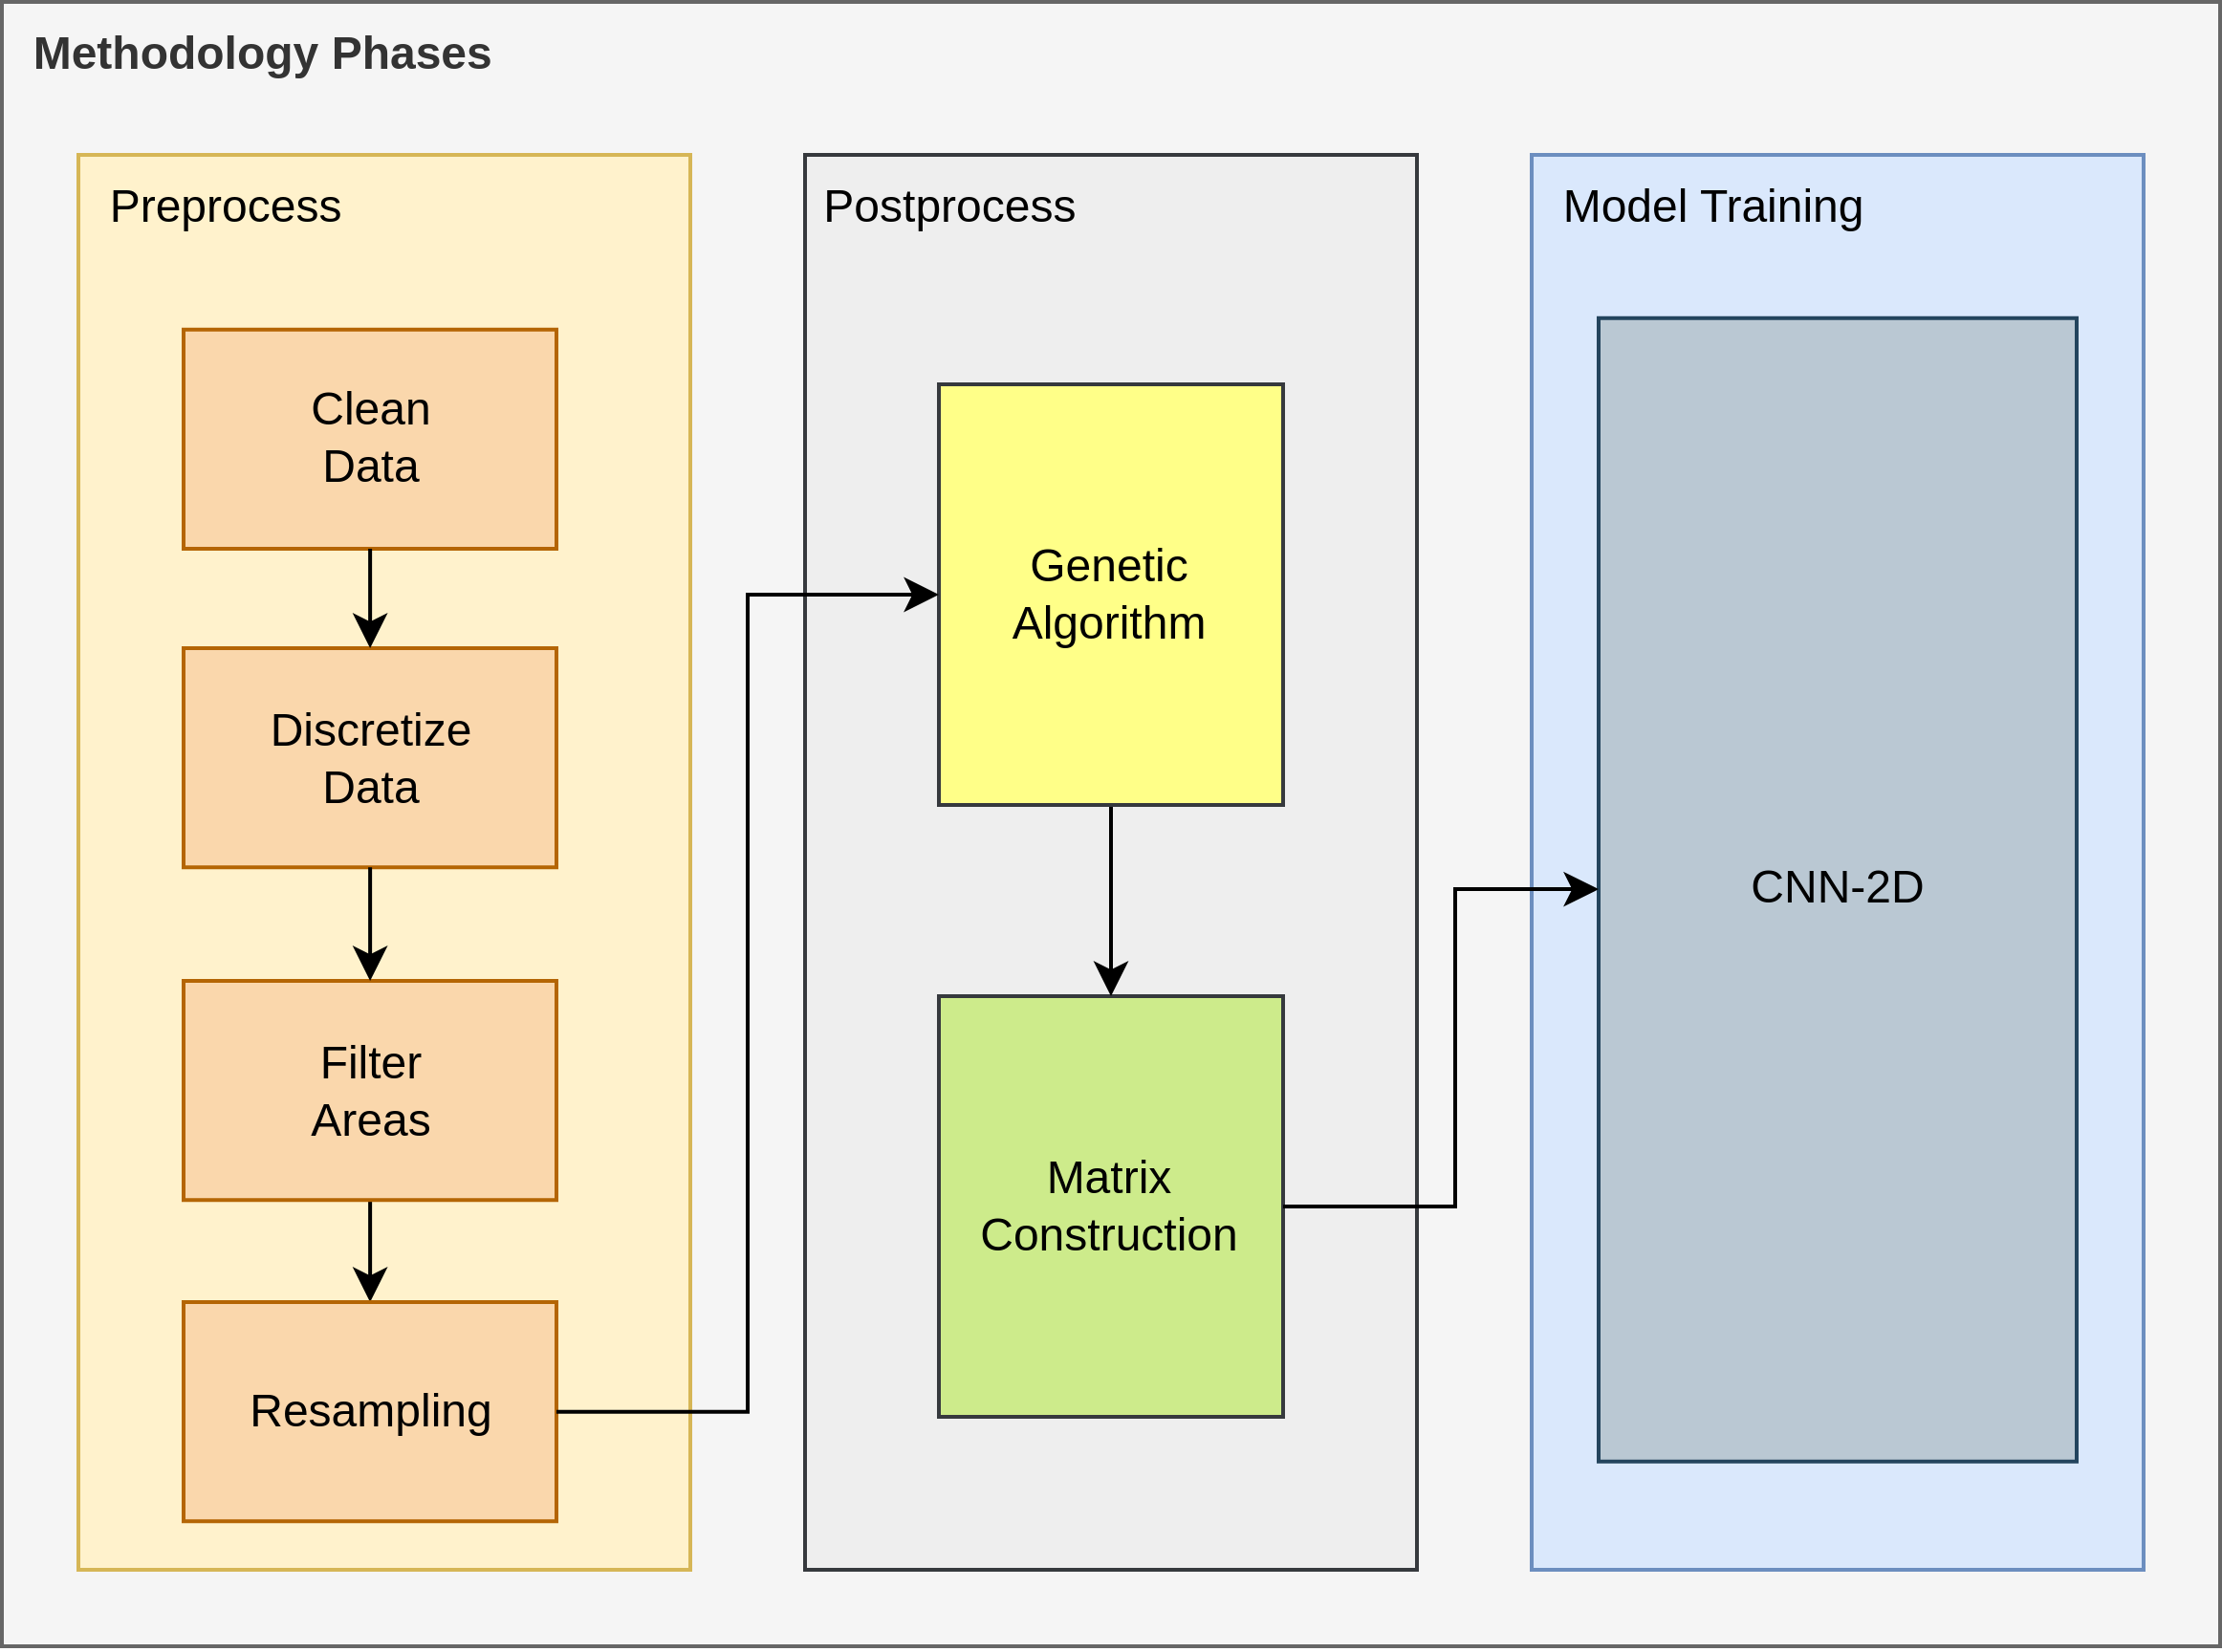
\includegraphics[width=14cm]{Figures/7th DataFlow Chart.png}
    \caption{Methodology flowchart: data preprocessing, postprocessing and model training.}
    \label{DataFlow}
\end{figure}

En segundo lugar, como segunda consideración importante respecto a la metodología prototipo, el concepto de gravedad de los accidentes es reasignado a dos clases (accidentes sin necesidad de asistencia y accidentes con necesidad). Esto se debe a que el valor que aporta distinguir entre la clases Severo y Fatal no es lo suficientemente enriquecedor como para arriesgarse a distinguir entre tres clases, ya que un modelo de clasificación a medida que incrementa el número de clases, tiene más posibilidades de realizar predicciones erróneas, sobre todo si son clases minoritarias como son los accidentes severos y fatales. Por este motivo se distinguen entre accidentes con necesidad de asistencia y aquellos que no.

\section{Preprocesamiento}

Esta sección explica las diferentes etapas que componen la fase de preprocesamiento de la metodología GTAAF propuesta. Esta es la primera de las etapas y es donde a los datos se les aplican transformaciones para dar lugar a un conjunto de datos refinado interpretable para cualquier modelo que trabaje con datos tabulares. Esta etapa está compuesta por cuatro fases: (1) proceso de limpieza de datos, donde se identifican, corrigen y se tratan las inconsistencias sobre los datos, (2) la discretización, donde se convierten las variables continuas en variables discretas y se codifican los valores cualitativos de las características, (3) el filtrado de áreas, donde se reduce el desbalanceo de los datos escogiendo subregiones de la ciudad donde se localicen ambos tipos de accidentes, y (4) el remuestreo, donde se se generan muestras sintéticas de la clase minoritaria para disponer de un dataset balanceado. En la Figura \ref{PreprocessingStage} se muestra el flujo sobre el que pasan los datos para cada una de las diferentes fases que componen la etapa de Preprocesamiento. Esta figura será referenciada en las siguientes subsecciones en la explicación de las fases de Preprocesamiento.

\begin{figure}[H]
    \centering
    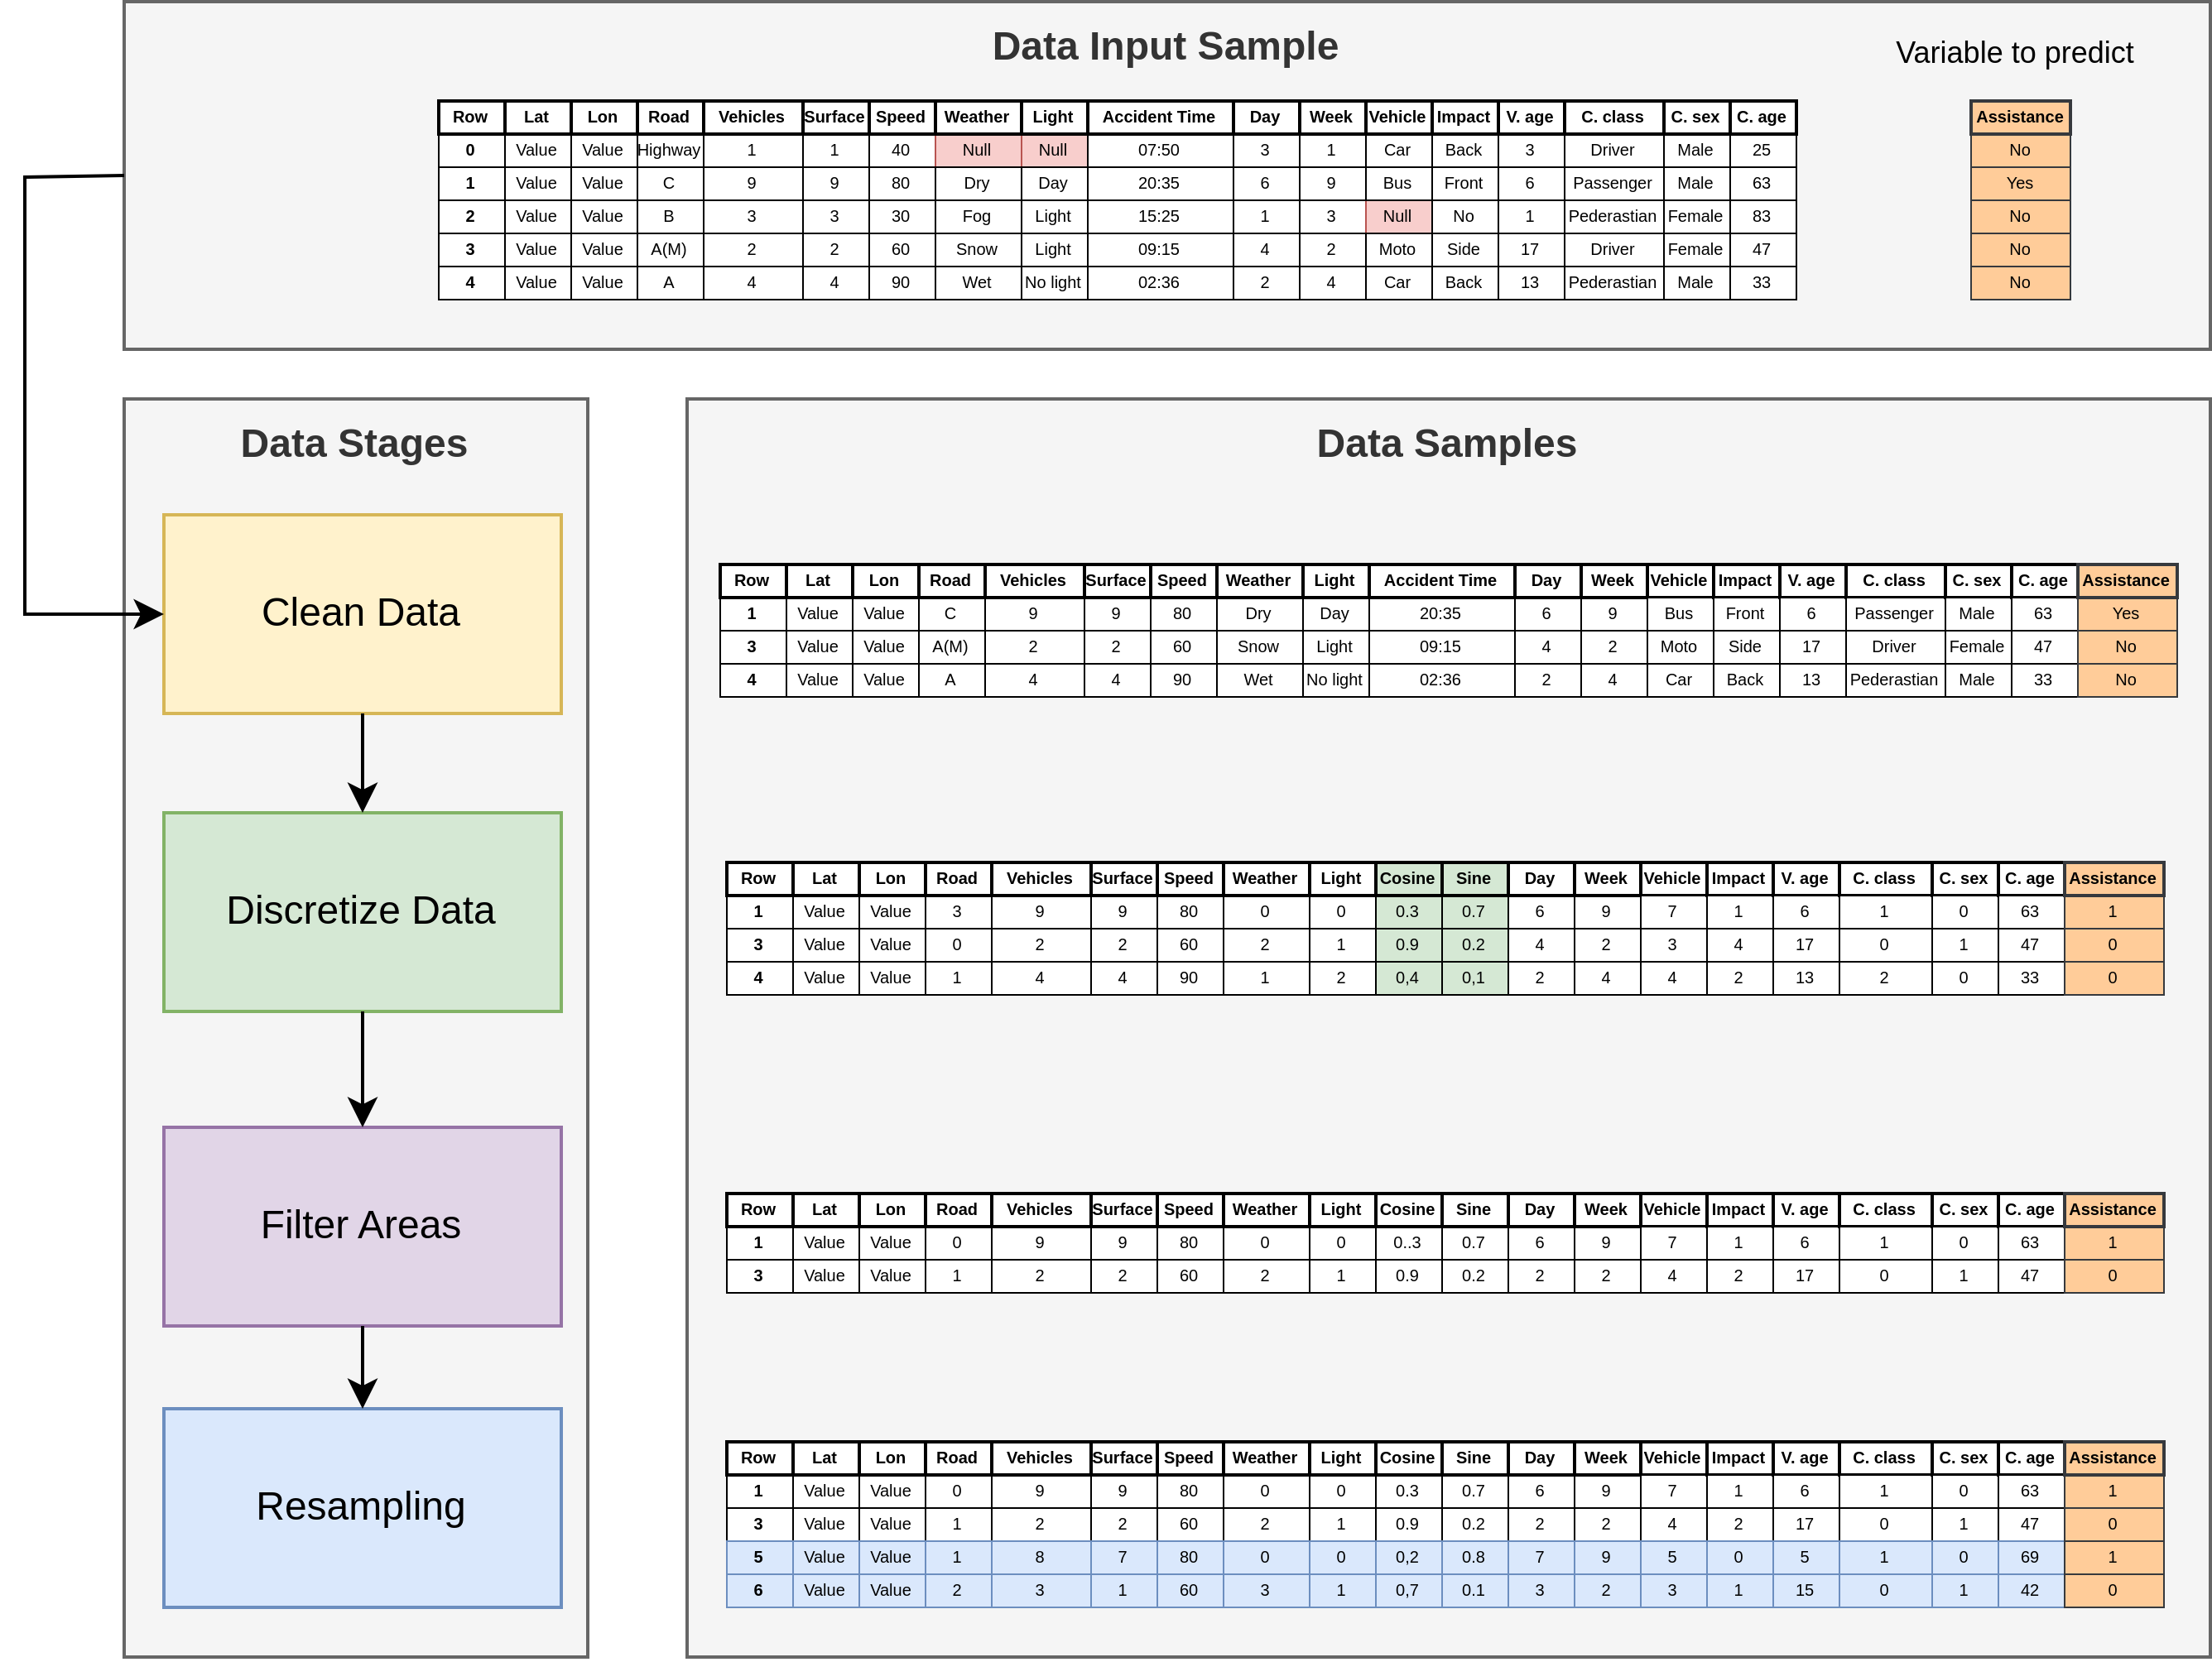
\includegraphics[width=17cm]{Figures/Preprocessing.png}
    \caption{Pre-processing data flow.}
    \label{PreprocessingStage}
\end{figure}


\subsection{Limpieza}

\textcolor{blue}{\textbf{Luis: es que aquí no hay mucho más que decir...}}\\

La limpieza de datos es un proceso esencial en cualquier proyecto de Análisis de datos o Inteligencia Artificial. Esta fase tiene como objetivo tratar los datos de tal forma que el dataset procesado no disponga de valores ausentes, atípicos,presenten inconsistencias o errores. Este proceso asegura que los datos estén listos para análisis y modelado. Un conjunto de datos limpio y refinado es la base para comenzar a trabajar con modelos predictivos, ya que de otra forma los datos no son fiables \cite{ilyas2019data}.


La primera fase de la metodología contempla un proceso de limpieza, en el que aquellos registros de los datos que presenten valores nulos o aquellos que se muestren atípicos sobre las variables escogidas serán eliminados del dataset. Esto provoca que haya un porcentaje de los datos que son eliminados. Estos casos se encuentran representados de color rojo en la primera etapa de la figura \ref{PreprocessingStage}, donde los registros de accidentes con identificador 0 y 2 son eliminados del conjunto de datos al presentar valores nulos en alguna de sus características.

\subsection{Discretización}


\textcolor{blue}{\textbf{Luis: con pinzas, no me termina de convencer, realmente no digo nada y no me gusta meter ejemplos de variables del dataset cuando aún no hemos presentado el dataset.}}\\

Los modelos predictivos trabajan con datos numéricos, que son los que son capaces de interpretar, sobre los que realizan operaciones matemáticas adquirir conocimiento sobre estos y poder realizar inferencias sobre muestras nunca antes vistas. Es por esto que las características ofrecidas en los conjuntos de datos deben ser transformadas a estos valores sin perder el valor que representa la información. A la hora de describir un accidente, gran parte de la información que se obtiene tiene una naturaleza cualitativa, es decir, son valores que no representan valores numéricos sino descriptivos. Esto se puede ejemplificar de forma clara con la característica 'First Point of Impact', en la que los valores que toma este campo en los conjuntos de datos originales representan una descripción del punto de impacto, como por ejemplo,  'Colisión frontal', 'Colisión lateral', etc. Por este motivo es necesario aplicar un proceso de discretización, este proceso busca transformar estos valores descriptivos a valores numéricos de tal forma que los datos puedan ser interpretados por los modelos, buscando representar de forma jerárquica la importancia de cada uno de los posibles valores descriptivos, teniendo como objetivo que la información descriptiva contenida sea coherente con su representación numérica.

% Por este motivo, en esta sección se expondrán el proceso que se ha seguido para transformar las variables cualitativas a cuantitativas, realizando una propuesta de cuantificación en la que se asigna un valor numérico a cada variable en función de la importancia dentro del total de valores que cada una de estas puede contener.

En esta tesis se ha seguido un procedimiento de discretización incremental, donde a cada posible valor del conjunto de datos se le ha asignado un valor numérico en función de la importancia que se le ha asignado.

\subsection{Transformación (Sin/Cos)}

\textcolor{blue}{\textbf{Luis: esto yo creo que estaría, a la espera de poner más bonito el dibujo.}}\\

Como se ha comentado en la sección anterior, los modelos de Inteligencia Artificial y Aprendizaje estadístico interpretan los datos en forma numérica. El valor numérico que se le asigna a cada campo es crítico, ya que será así como el modelo interprente el orden de los valores cualitativos que los humanos somos capaces de comprender. La representación del formato de la horas y minutos del día, por su naturaleza, no es una excepción. El concepto de la hora del día tiene un componente cíclico que es necesario representar para que el modelo comprenda que las once y cincuentainueve de la noche es una hora muy próximas a las doce de la noche. Esto es algo a lo que los seres humanos estamos acostumbrados, pero debe ser indicado de forma coherente para los modelos de IA que intepretarían que estas dos horas muy parejas son valores totalmente opuestos en los posibles valores que puede contener la característica hora con el formato 24 hroas que conocemos (23:59, 00:00). Con el objetivo de representar de forma consistente la información de la hora del accidente, es necesario aplicar una transformación que interprete las horas y minutos en formato 24h a un formato cíclico, y para ello se transformará este campo inicialmente de una dimensión, a dos dimensiones sinusoidales. Para realizar este proceso en primer lugar se transforma la hora y el minuto en el que se ha producido cada accidnete a segundos. Posteriormente se aplican las siguientes fórmulas sobre los segundos para representar la hora del accidente en dos componentes, el senosoidal y el cosenoidal:


\begin{center}
    $\sin((2 \cdot \pi \cdot DaySeconds)/SecondsInDay)$
    
    $\cos((2 \cdot \pi \cdot DaySeconds)/SecondsInDay)$
\end{center}

(Dibujito explicativo de senos y cosenos)[puedo poner las 23:59 de la noche representada en seno y coseno, las 00:00 y las 15:00 para que se vean las diferencias]. En la figura \ref{HoursPlot} se muestra un ejemplo de la naturaleza cíclica de la representación de la variable Hora en forma de seno (eje de ordenadas) y coseno (eje de coordenadas), donde se observa que la hora 00:00 en el espacio bidimensional se encuentra más cercana a la hora 07:58:00 respecto a cualquier otra posible representación unidimensional.

\begin{figure}[H]
    \centering
    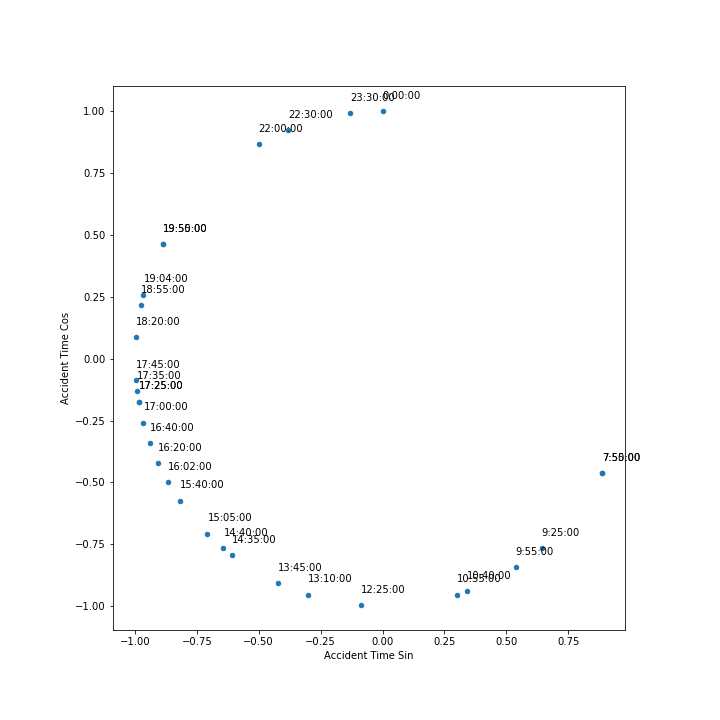
\includegraphics[width=7cm]{Figures/hours.png}
    \caption{Algo así, no es lo definitivo.}
    \label{HoursPlot}
\end{figure}

En la Figura \ref{PreprocessingStage} de referencia, se muestra el ejemplo donde el accidente sin necesidad de asistencia con identificador 4 se elimina del conjunto de datos porque no convive con otro accidente de tipo asistencia dentro de su mismo área.

\subsection{Fitrado de Áreas}

\textcolor{blue}{\textbf{Luis: esto yo creo que estaría.}}\\

Uno de los retos más comunes en el campo de la Inteligencia Artificial es disponer de un conjunto de datos no balanceado. Este problema implica tener una desproporción del número de muestras en base a la variable a predecir. Esta casuística afecta negativamente al entrenamiento de los modelos de Inteligencia Artificial, ya que estos en su etapa de entrenamiento adquieren el conocimiento prediciendo sobre estas muestras y son penalizados cuando sus predicciones durante esta fase son erróneas. Si la distribución de datos de entrenamiento dispone de muchas más muestras de una clase que de otra, el modelo tenderá a aprender durante su entrenamiento a predecir siempre aquella clase mayoritaria, ya que se le ha penalizado en menos ocasiones durante esta fase, obteniendo así un modelo sesgado que está condicionado por naturaleza a predecir sobre la clase más común.

En lo que respecta la naturaleza de la distribución de datos de accidentes de tráfico, siempre existirán muchos más accidentes que no han necesitado asistencia respecto a los que sí. Por lo que durante esta fase de la metodología se busca paliar este efecto tratando de reducir la diferencia entre el número de registros de la clase mayoritaria (sin necesidad de asistencia) y la clase minoritaria (necesidad de asistencia).

Para solventar esto se aplica un filtrado basado en áreas, que buscará balancear los datos escogiendo áreas estratégicas donde coexistan accidentes con ambos tipos de consecuencias. Para cada población se establece una ventana de dimensiones (X,Y) que recorrerá secuencialmente el área total que engloba cada una de las regiones escogidas en esta tesis. Esta ventana buscará si en ese área coexisten accidentes de tipo No-Asistencia y Asistencia, de tal forma que si esto se cumple, dicha subárea se mantendrá en el dataset, y en caso contrario se eliminará. Esto consigue un balanceo de los datos que minimiza el número de accidentes de tipo No-Asistencia en el dataset que no sean estrictamente necesarios. En la figura \ref{Areas} se muestra un ejemplo del criterio seguido para aplicar este filtrado, donde se seleccionan únicamente aquellas regiones donde coexisten accidentes sin necesidad de asistencia (verde) y con necesidad de asistencia (rojo).

\begin{figure}[H]
    \centering    

    \subfigure[Example of dataset accidents points.]{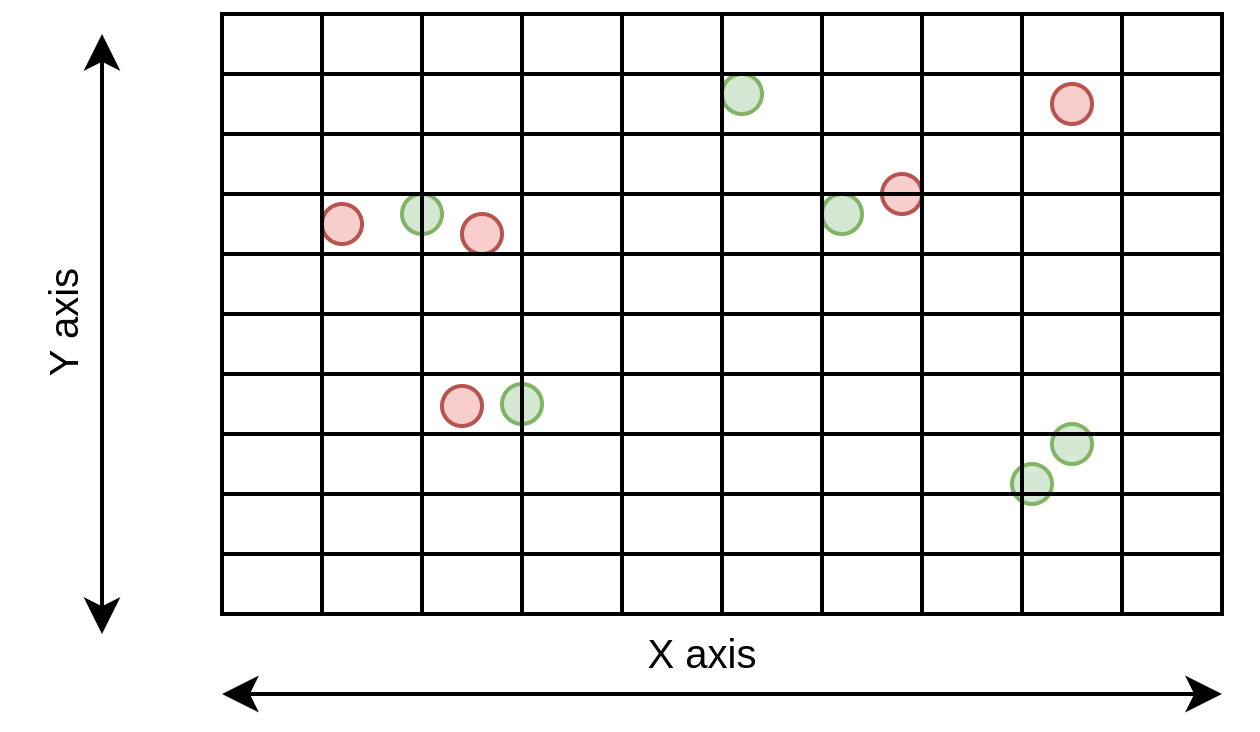
\includegraphics[width=6cm]{Figures/areas-points.png}}
    \subfigure[Example of filtered dataset accidents points.]{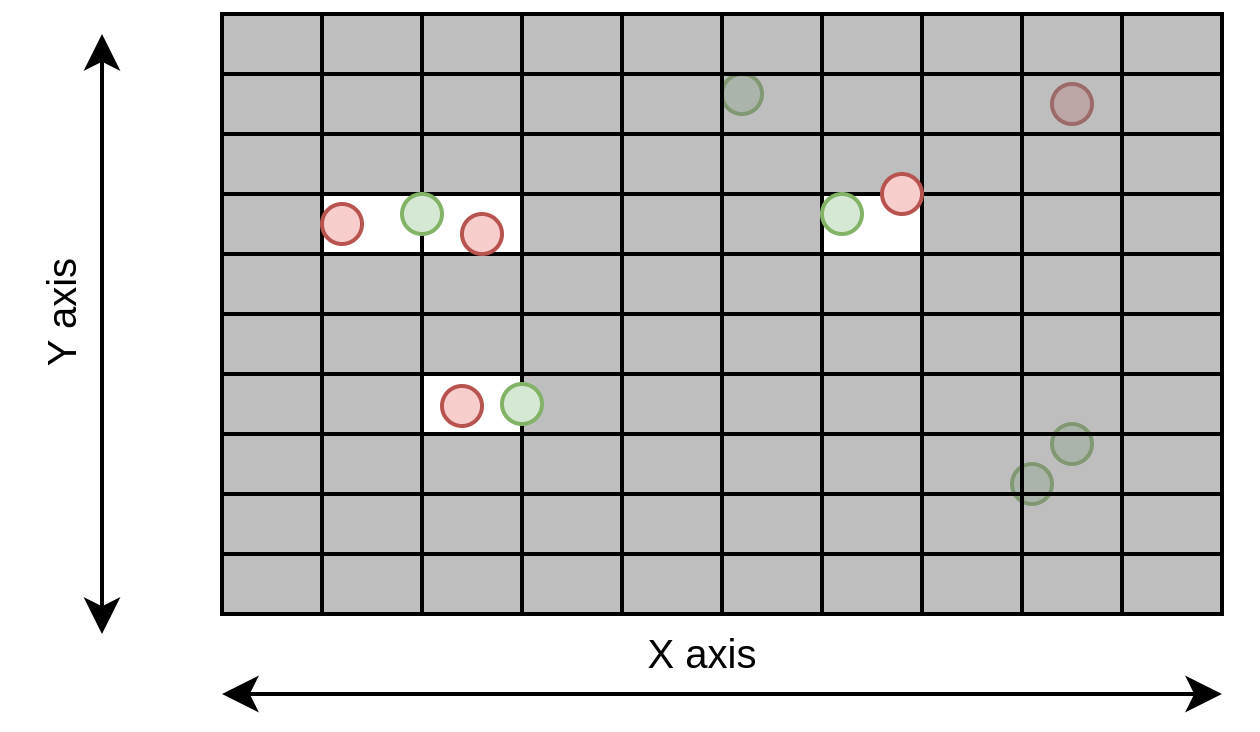
\includegraphics[width=6cm]{Figures/areas-points-filtered.png}}
    \label{Areas}
    \caption{Ejemplo de filtrado de áreas. Los puntos verdes representan accidentes con lesiones leves, mientras que los puntos rojos representan accidentes que requirieron asistencia.}
\end{figure}

En la Figura \ref{PreprocessingStage} de referencia, se muestra el ejemplo donde el accidente sin necesidad de asistencia con identificador 4 se elimina del conjunto de datos porque no convive con otro accidente de tipo asistencia dentro de su mismo área.

\subsection{Normalización}

\textcolor{blue}{\textbf{Luis: esto yo creo que estaría, no se me ocurre qué más poner, no obstante no me convence poner ejemplos de los datasets cuando aún no los hemos presentado.}}\\

En cualquier modelo de Inteligencia Artificial es imprescindible normalizar los datos. Los modelos de Inteligencia Artificial trabajan con valores numéricos realizando operaciones sobre ellos. En los conjuntos de datos suelen coexistir variables cuyos valores se encuentran representados en distintas escalas, es decir, que los valores que pueden tomar ciertas característica suelen presentar un rango de valores mucho más amplio que otras de ellas dentro del mismo conjunto de datos, haciendo que las características sean incomparables entre sí debido a su magnitud. Un ejemplo de esto puede observarse en la características 'Semana en Año' y 'Sexo', la primera de estas variables puede contener un amplio conjunto de posibles valores (desde el 0 hasta el 51), en función de la semana en la que se ha producido el accidente, mientras que la segunda variable únicamente puede tomar dos valores (0 ó 1). Esta variabilidad numérica en los posibles valores de los datos provoca que las operaciones matemáticas que aplican los modelos durante su fase de entrenamiento sean desproporcionadas en las características con rango de valores más altos, produciendo una desproporción en estas operaciones, haciendo los datos incomparables enre sí, dándole más importancia a unas características que a otras. Es por esto por lo que es necesario un proceso de logre acotar el rango de posibles valores del conjunto total de datos. Existen distintas técnicas para aplicar la normalización en los datos, Existen diferentes técnicas de normalización como Mean Centered (MC), Variable Stability Scaling (VSS) o Min-Max Normalization (MMN), entre otras \cite{DataNormalizationInvestigation}. . En esta tesis, para normalizar los datos y hacerlos comparables entre sí se ha utilizado la técnica de Z-Score (ZSN) debido a que logra representaciones de acuerdo con una distribución normal. Para hacerlo, se utilizan la media y la desviación estándar para reescalar los datos de manera que su distribución esté definida por una media de cero y una desviación estándar unitaria.


\begin{center}
    $Z = \frac{(X - \mu)}{\sigma}$
\end{center}


\subsection{División Train-Val-Test}

\textcolor{blue}{\textbf{Luis: esto yo creo que estaría, lo único hacer inciso en lo último.}}\\

Los modelos supervisados de Inteligencia Artficial aprenden patrones sobre datos que son ofrecidos en la etapa de entrenamiento del modelo. Durante esta fase los modelos realizan predicciones sobre de datos y posteriormente se les enseña la clase a la que pertenecía cada uno de los datos que ha predicho, de esta forma se mide el error que han cometido durante este proceso y los pesos de la red son actualizados para minimizar el error en la siguiente fase. Si este aprendizaje se repite durante muchas etapas, el modelo tiende a aprenderse los datos de memoria, lo que se conoce como sobreajuste de la red u overtfitting, provocando que la red no sea capaz de generalizar ante nuevas muestras tras su entrenamiento. Por este motivo es importante mantener el control del entrenamiento de la red mediante la evaluación del rendimiento de la red en cada época mediante un conjunto de datos que nunca ha visto durante sus fases de entrenamiento, este conjunto de datos es conocido como conjunto de validación, y es utilizado para parar el entrenamietno cuando el modelo no sea capaz de generalizar sobre estas muestras. Por otra parte, existe el conjunto un conjunto de datos de test, utilizado para medir el rendimiento del modelo final una vez ha acabado su fase de entrenamiento. Este conjunto pertenece a muestras que la red no ha visto durante su fase de aprendizaje ni ha sido utilizado como validación.

En esta tesis se ha dividido el conjunto de datos original de cada una de las ciudades mediante... (80\% lo normal..)

\subsection{Resampling}

\textcolor{blue}{\textbf{Luis: no me termina de convencer, estoy presentando métodos de resampling para justificar por qué usamos el SMOTE, pero me da la sensación de que colapsaría con el estaod del arte si incluyésemos esto ahí.}}\\

El conjunto de datos, una vez se han reducido considerablemente el desbalanceo entre las dos clases gracias al proceso de filtrado de áreas, sigue presentando cierto desbalanceo. Por mucho que se haya acotado el problema a regiones individuales, es lógico que se hayan producido mas accidentes sin necesidad de asistencia respecto a las que sí. En problemas de Inteligencia Artificial y Aprendizaje Estadístico es común aplicar técnicas que permitan igualar el número de muestras en conjuntos de datos donde se presenta desbalanceo. Existen dos principales corrientes que tienen como objetivo reducir la diferencia del desbalanceo de los datos. La primera de ellas consiste en igualar el número de muestras de la clase minoritaria hasta llegar a la mayoritaria (upsampling) mediante técnicas de reemplazamiento de datos (resamping), tal y tal . La segunda filosofía consiste en eliminar aleatoriamente registros de la clase mayoritaria hasta llegar al número de la minoritaria (undersamping) \cite{mohammed2020machine}. De esta forma se consigue un dataset balanceado que no provoque un sesgo en el entrenamiento de la red. En el caso de estudio de esta tesis, aplicar técnicas que eliminen accidentes sin necesidad de asistencia hasta igualar el número de aquellos que sí la requieren es un inconveniente, ya que al disponer de tan pocas muestras de la segunda clase, el conjunto de datos resultante se vería notablemente reducido, lo que afectaría negativamente al entrenamiento de la red, que requiere de un conjunto de datos lo más extenso posible para favorecer la generalización en sus predicciones. Por este motivo, en esta tesis se opta por métodos de aumentado de datos (upsampling), que mantienen el valor que aportan las muestras de los accidentes sin necesidad de asistencia, aumentando los datos de aquellos que sí la requieren. Contras del resampling... Por estos motivos en este trabajo se ha optado por una técnica de generación de datos sintética denominada Synthetic Minority Oversampling Technique (SMOTE-II), que busca incrementar el número de clases de las muestras minoritarias mediante la generación de nuevas muestras artificiales.

Para la generación de nuevas muestras sintética mediante SMOTE-II, se hace uso del espacio de caracteŕisticas, para generar nuevas muestras de la clase mayoritaria que se encuentren cercanas al espacio de características que divide ambas clases. Para ello, se proyecta una nueva muestra de la clase minoritaria entre la línea que divide una muestra aleatoria respecto a uno de sus vecinos más cercanos.

Esta técnica permite generar datos sintéticos en base al contexto que conforman las muestras de la clase minoritaria hasta llegar a la mayoritaria.

En la Figura \ref{PreprocessingStage} de referencia se observa, marcados en azul, cómo los registros con identificadores 5 y 6 han sido generados en base a las modificaciones de los valores de los registros 1 y 3 para balancear el dataset.


\section{Postprocesamiento}

La segunda fase de la metodología implica transformar los datos refinados y balanceados en matrices interpretables por el modelo GTAAF recién propuesto. Este proceso implica mapear los atributos de las muestras tabulares en posiciones dentro de estas matrices. Para realizar esto, se hará uso de un método de transformación que toma en consideración la importancia de cada característica dentro del conjunto de datos. El objetivo es posicionar estratégicamente las características más relevantes en la matriz para maximizar su impacto en el modelo GTAAF, como se ilustra en la Figura \ref{PostprocessingStage}. La determinación de la importancia de las características se basa en un algoritmo tipo boosting, que asigna pesos a las características según su relevancia en la separación de datos durante el entrenamiento. Para garantizar un entrenamiento óptimo del modelo, se realiza una optimización de hiperparámetros utilizando un algoritmo genético. A lo largo de generaciones sucesivas, este algoritmo genético hace evolucionar los hiperparámetros, guiado por la métrica de F1-Score, que actúa como la función heurística.

\begin{figure}[H]
    \centering
    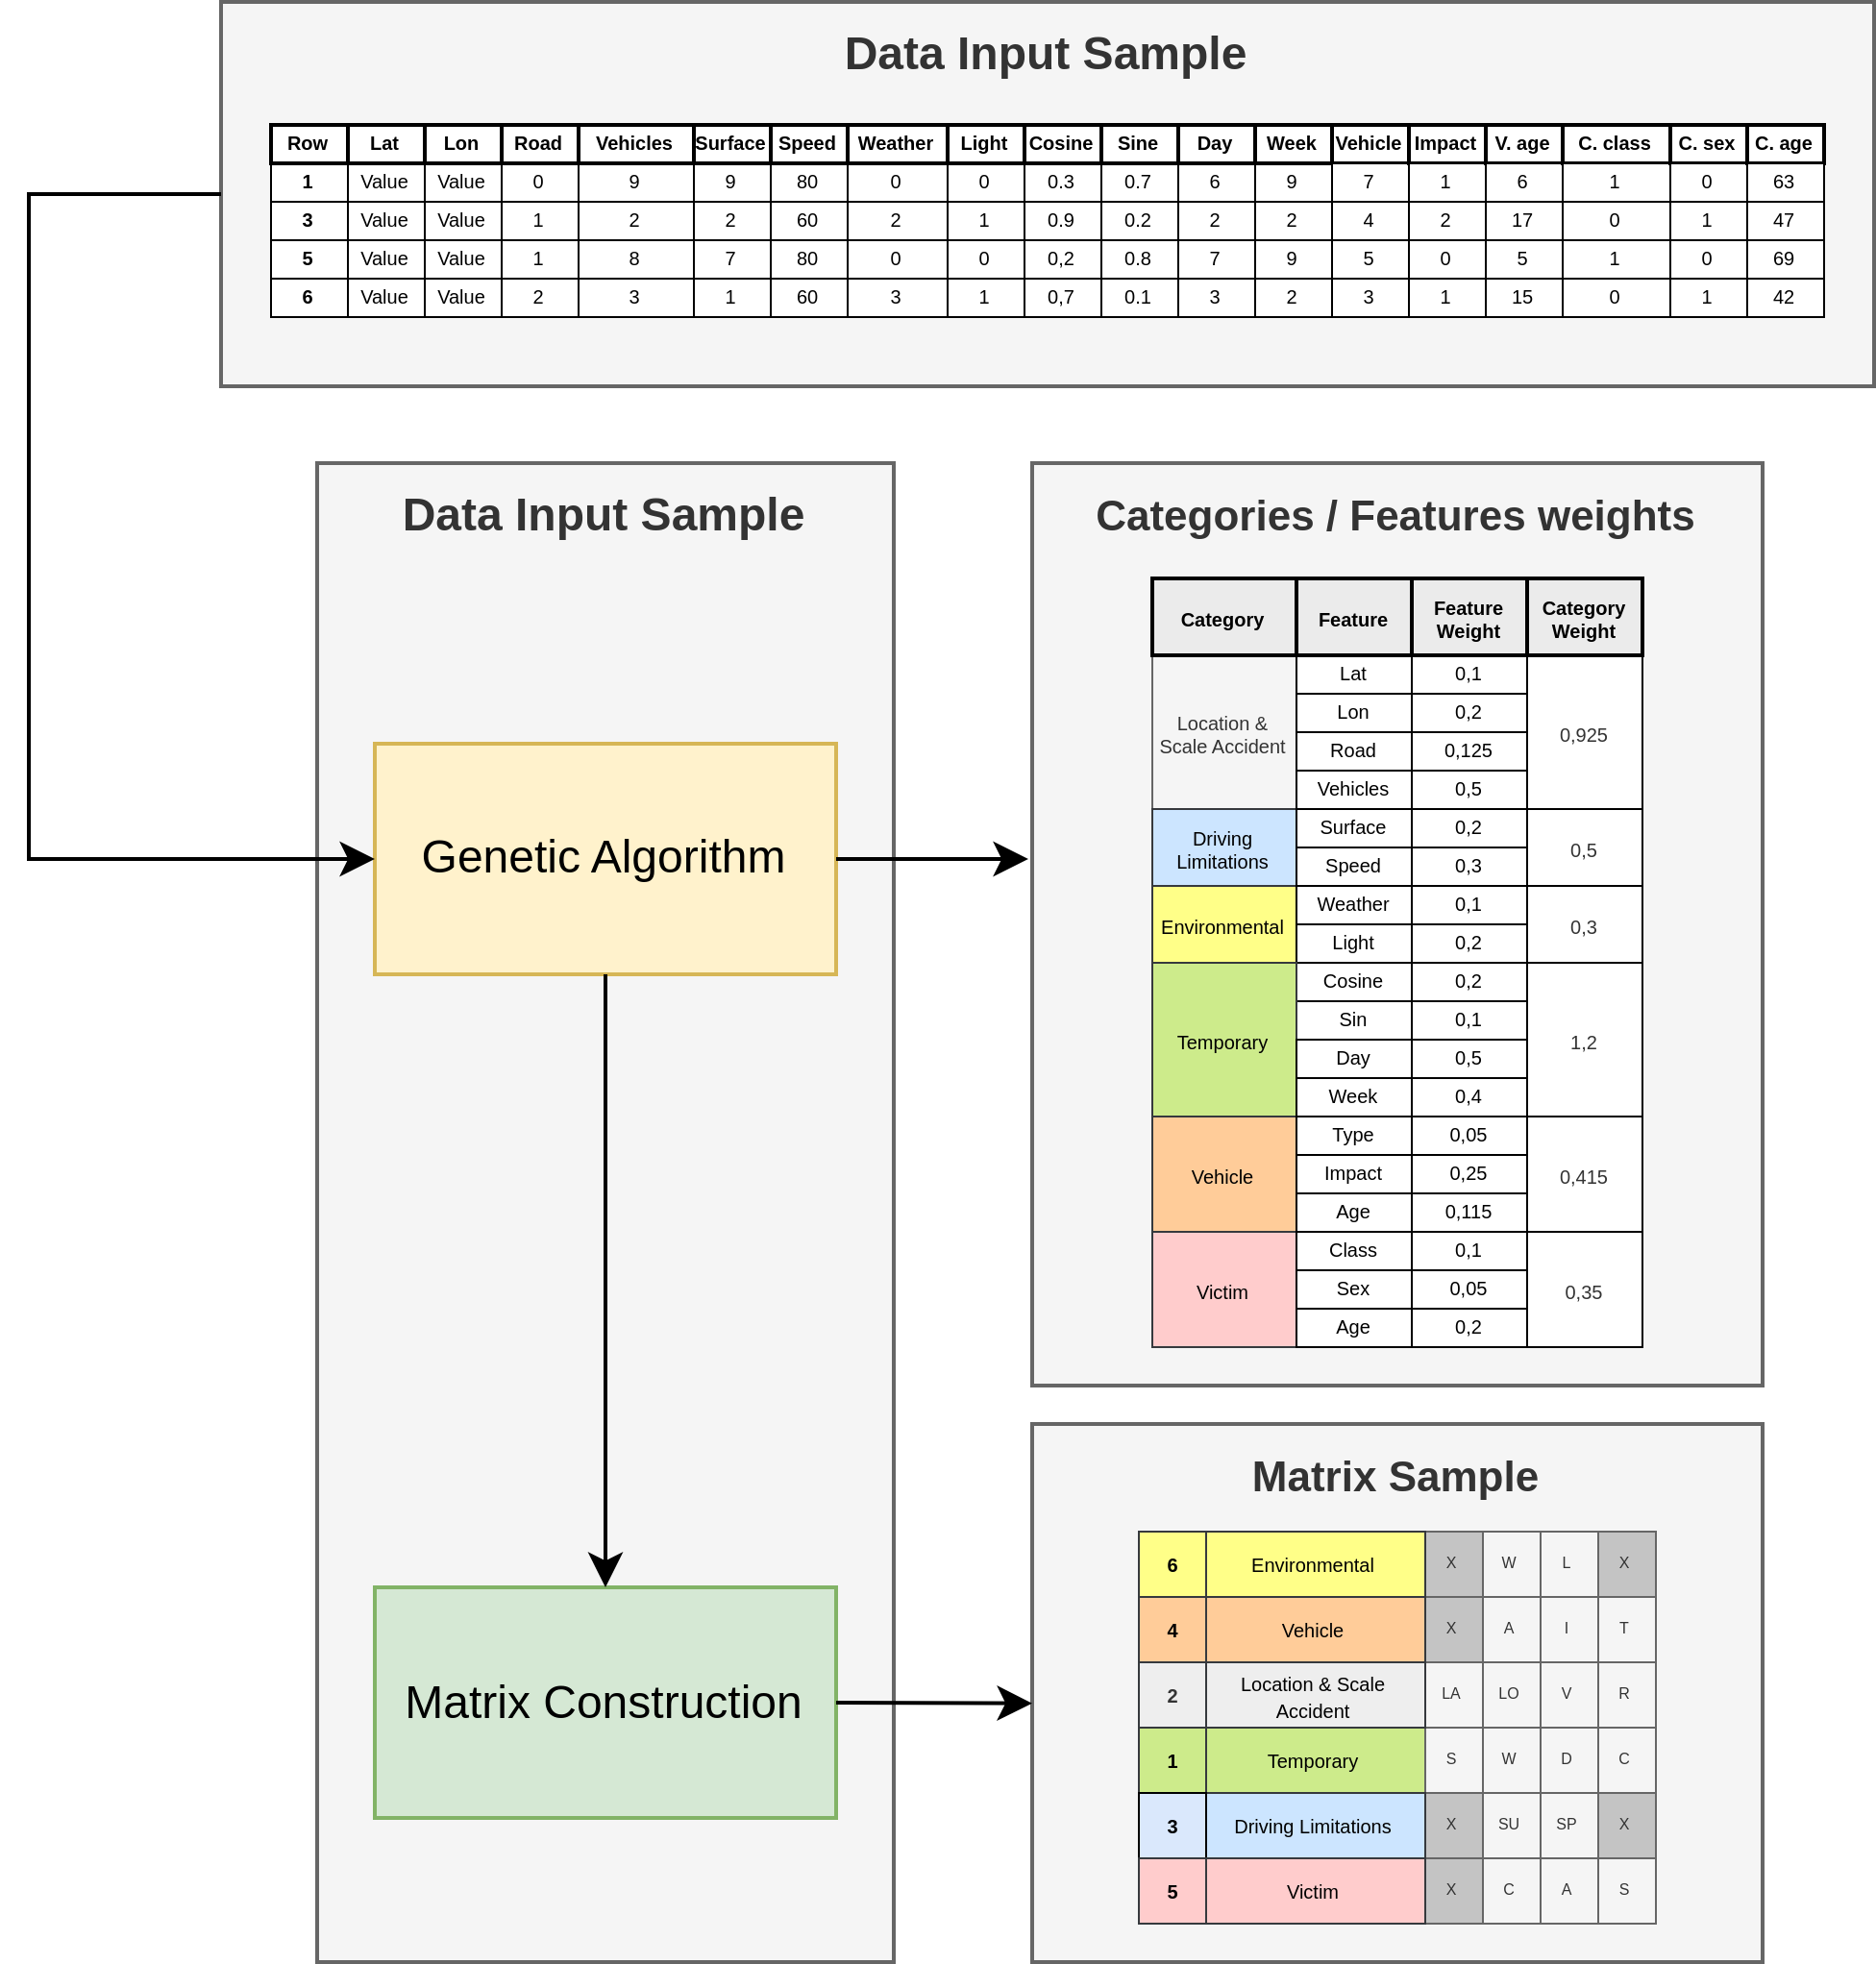
\includegraphics[width=14cm]{Figures/Postprocessing_2.png}
    \caption{Category and feature weights.}
    \label{PostprocessingStage}
\end{figure}

\subsection{Construcción de Matrices}

\textcolor{blue}{\textbf{Luis: este es el tinte que le quiero un poco dar, justificar por qué usamos lo que usamos y sobre todo justificar por qué no usamos otros métodos del estado del arte.}}\\

En esta tesis, se presenta un método para construir datos inicialmente tabulares a datos matriciales con los que podrá trabajar el modelo convolucional propuesto, esta transformación hace uso de la categorización de las características y la importancia de cada una de ellas individualmente dentro del conjunto de datos a las que pertenecen. En la sección X se explicó el funcionamiento del proceso de categorización propuesto, que buscaba poder aplicar esta metodología a cualquier conjunto de datos de accidentes agrupando las características en conceptos básicos y de fácil categorización. El siguiente paso para lograr la transformación de los datos inicialmente en filas y columnas a datos matriciales es asignar cada una de las características del conjunto de datos a una posición dentro de la matriz, de tal forma que los datos puedan ser interpretados por el modelo convolucional. Para tener un contexto de la importancia en el orden en el que se asignan estas características, se explica brevemente la intuición sobre la que trabajan las redes neuronales convolucionales. Los píxeles que componen una imagen representan patrones que, para los seres humanos, son reconocibles, las redes convolucionales aprenden a reconocer estas variaciones, inicialmente en una escala pequeña (pocos píxeles), y, a medida que aumenta el número de capas, estas redes son capaces de aprender patrones más complejos en base a la composición del reconocimiento de aquellos más simples. Este funcionamiento, por definición, implica que la forma en la que se compone una imagen sea crítica, es decir, que el contenido que representa la imagen debe estar formado de manera coherente para que las redes puedan aprender estos patrones, requiriendo un sentido y/o contexto completo en su composición.

Existen distintos métodos que logran transformar datos tabulares a una representación matricial de los mismos, buscando dar un sentido a la asignación de las características en posiciones de la matriz. En la sección \ref{SOAT_MATRIX_ALGORITHM_CONSTRUCTION} se presentaron distintos métodos como REFINED, DeepInsight o IGTD, que buscan optimizar la posición de las características en base a la similaridad que presenten entre ellas, principalmente en datos orientados a la descripción genética. Sin embargo, estas técnicas presentan distintas limitaciones debido a la magnitud de los datos para las que han sido diseñadas (del orden de 2.500 características), esto provoca que estos métodos sean difícilmente aplicables a datos de baja dimensionalidad, como asignar espacios en blanco ante la falta de características o que los métodos no sean capaces de converger al trabajar con tan pocos datos. En el caso de estudio de esta tesis las características disponibles son mucho menores, del orden de 20 variables.

Debido a las limitaciones de los métodos anteriores, en esta tesis se presenta un método de composición de matrices en base a la importancia de las características, que permite asignar cada una de las variables del dataset a posiciones estratégicas dentro de la matriz haciendo uso de dos conceptos fundamentales, los Algoritmos Genéticos y los Algoritmos de Medición de Importancia de Características (feature importance).




\subsection{Feature Importance Algorithm}

\textcolor{blue}{\textbf{Luis: Floja la justificación, pero van por ahí los tiros.}}\\

Como se ha presentado en la sección \ref{SOAT_FEATURE_IMPORTANCE_METHODS}, existen distintos métodos que permiten evaluar la importancia de las variables en función de distintos criterios, como la correlación que presentan las variables entre sí o el nivel de importancia de cada característica a la hora de entrenar un modelo predictivo, ejemplos como estos son la Regresión Logística, técnicas de ensembles de tipo Bagging como los Random Forest o métodos ensembles tipo Boosting.


En esta tesis se trabaja con un dataset desbalanceado, por lo que a la hora de aplicar algoritmos de medición de características es importante escoger técnicas que sean insensibles a esto. Una de las muchas propiedades que ofrecen de los métodos de ensembles es que se adaptan especialmente bien a conjuntos de datos sesgados. Estos modelos, en sus distintas formas, se benefician de estar compuestos de una combinación de modelos y distintas técnicas de muestreo que reducen considerablemente el sobreajuste que pueda darse con otros métodos.

Dentro de estos modelos, los ensembles tipo Boosting son ampliamente conocidos por adaptarse especialmente bien en estos casos. Estos modelos utilizan técnicas de regularización durante su entrenamiento y se centran en minimizar el error producido cuando clasifican muestras de aquellas clases más conflictivas, que en el caso de un dataset desbalanceado serán las muestras minoritarias. Por otra parte, son modelos muy robustos que generalmente ofrecen un mayor rendimiento respecto a otros tipos de ensembles como los Random Forest, que únicamente ofrece que cada uno de los modelos sea entrenado con un subconjunto de los datos originales.

En esta metodología se utilizará el algoritmo tipo Boosting XGBoost, donde se minimizará la métrica F1-Score resultante de la clasificación de ambas clases de accidentes (Sin necesidad de asistencia y necesidad de asistencia). La principal limitación de este algoritmo para ofrecer un buen rendimiento es que requiere de una optimización de hiperparámetros con los que se entrenan los datos. % Para buscar una configuración adecuada de este método, se aplicarán algoritmos genéticos.


% Existen múltiples algoritmos que implementan esta filosofía, entre los que destacan: (1) AdaBoost, orientado a clasificación, que en cada iteración , (2) Random Forest () y (3) XGboost. Para la metodología presentada en esta tesis se ha escogido la técnica XGBoost, ya que las características de este algoritmo son las más adecuadas a este contexto. XGBoost es menos sensible a datos que presentan una alta variabilidad y un importante desbalanceo entre ellos. Además, este algoritmo permite una mejor optimización en sus árboles sucesores al configurar los hiperparámetros con los que se entrena únicamente una única vez para el árbol inicial (profundidad del árbol, número de árboles y learning rate) [2]. El funcionamiento del XGBoost escogido es el siguiente...
 


\subsection{Algoritmo Genético}
\textcolor{green}{Explicar qué métodos existen para optimizar hiperparámetros, por qué no nos sirven (costes computacionales) y por qué optamos por algoritmos genéticos (son muy buenos sin necesidad de hacer fuerza bruta)}\\

\textcolor{blue}{\textbf{Luis: Ni leerlo, tengo que }}\\

Como se ha comentado en la sección \ref{HYPERPARAMETERS_OPTIMIZATION_METHODS}, existen numerosos métodos para optimizar hiperparámetros...

Es por esto por lo que en esta tesis, los algoritmos genéticos son utilizados para optimizar los hiperparámetros de entrenamiento del algoritmo XGBoost, que ofrecerá la importancia de las características, necesaria para la construcción de las matrices de entrada a la red CNN-2D propuesta. Donde cada uno de los individuos de la población del algoritmo genético representará una posible combinación de hiperparámetros, concretamente los valores de (Max Depth, ETA y N árboles). La función heurística que será optimizada será el F1-Score otorgado sobre los datos de test de cada uno de los conjuntos de datos.



\subsection{Construcción de Matrices}

Una vez se dispone de la categorización de los datos y de los pesos de las características gracias al modelo XGBoost, se aplica el proceso de asignación de cada una de las variables a posiciones de la matriz. Como se ha comentado en secciones anteriores, la forma en la que se compone una matriz sobre la que opera una red convolucional es de vital importancia, los filtros que estas aprenden \textcolor{green}{seguir}.... \textcolor{red}{Aquí otra vez?: Existen diferentes enfoques para construir matrices en base a datos tabulares, pero estos enfoques como se ha comentado en la sección XX sufren de limitaciones aplicados a nuestro caso de eso, (dimensiones de los datos, etc. ensar algo)} . Por este motivo se ha diseñado una estrategia que pretende posicionar las características más relevantes de cualquier conjunto de datos (definidas por el algoritmo XGBoost) a posiciones cercanas al centro de la matriz, que son las que... Este proceso teniendo en cuenta la categorización inicial que permite aplicar esta metodología a cualquier región, siendo tolerante a la falta de características en la disponibilidad de los datos que se ofrezcan.

El método diseñado sigue los siguientes pasos:

\begin{enumerate}
    \item En primer lugar, las características son asociadas a sus categorías, de tal forma que pueda medirse la importancia de cada categoría dentro del conjunto de datos. Esta es obtenida mediante la suma del peso total de cada característica individual que la contiene
    \item El segundo paso es asignar cada categoría con una fila de la matriz según su peso, donde aquella con el mayor peso se posiciona en la fila central, la segunda categoría más importante se asocia a la fila inmediatamente superior, la siguiente a la fila inmediatamente inferior y así sucesivamente (ver Figura \ref{CategoriesFeaturesWeights}).
    \item Una vez que las categorías están asociadas a una fila de la matriz, cada una de las características dentro de su categoría se asocia en cada columna siguiendo el mismo procedimiento definido en el apartado anterior. La característica más importante de una categoría se posiciona en el centro, la segunda característica más importante se sitúa inmediatamente a su izquierda, mientras que la siguiente característica más importante ocupa el lugar a su izquierda y así sucesivamente (ver Figura \ref{MatrixIndexes}).
\end{enumerate}


\begin{figure}[H]
    \centering
    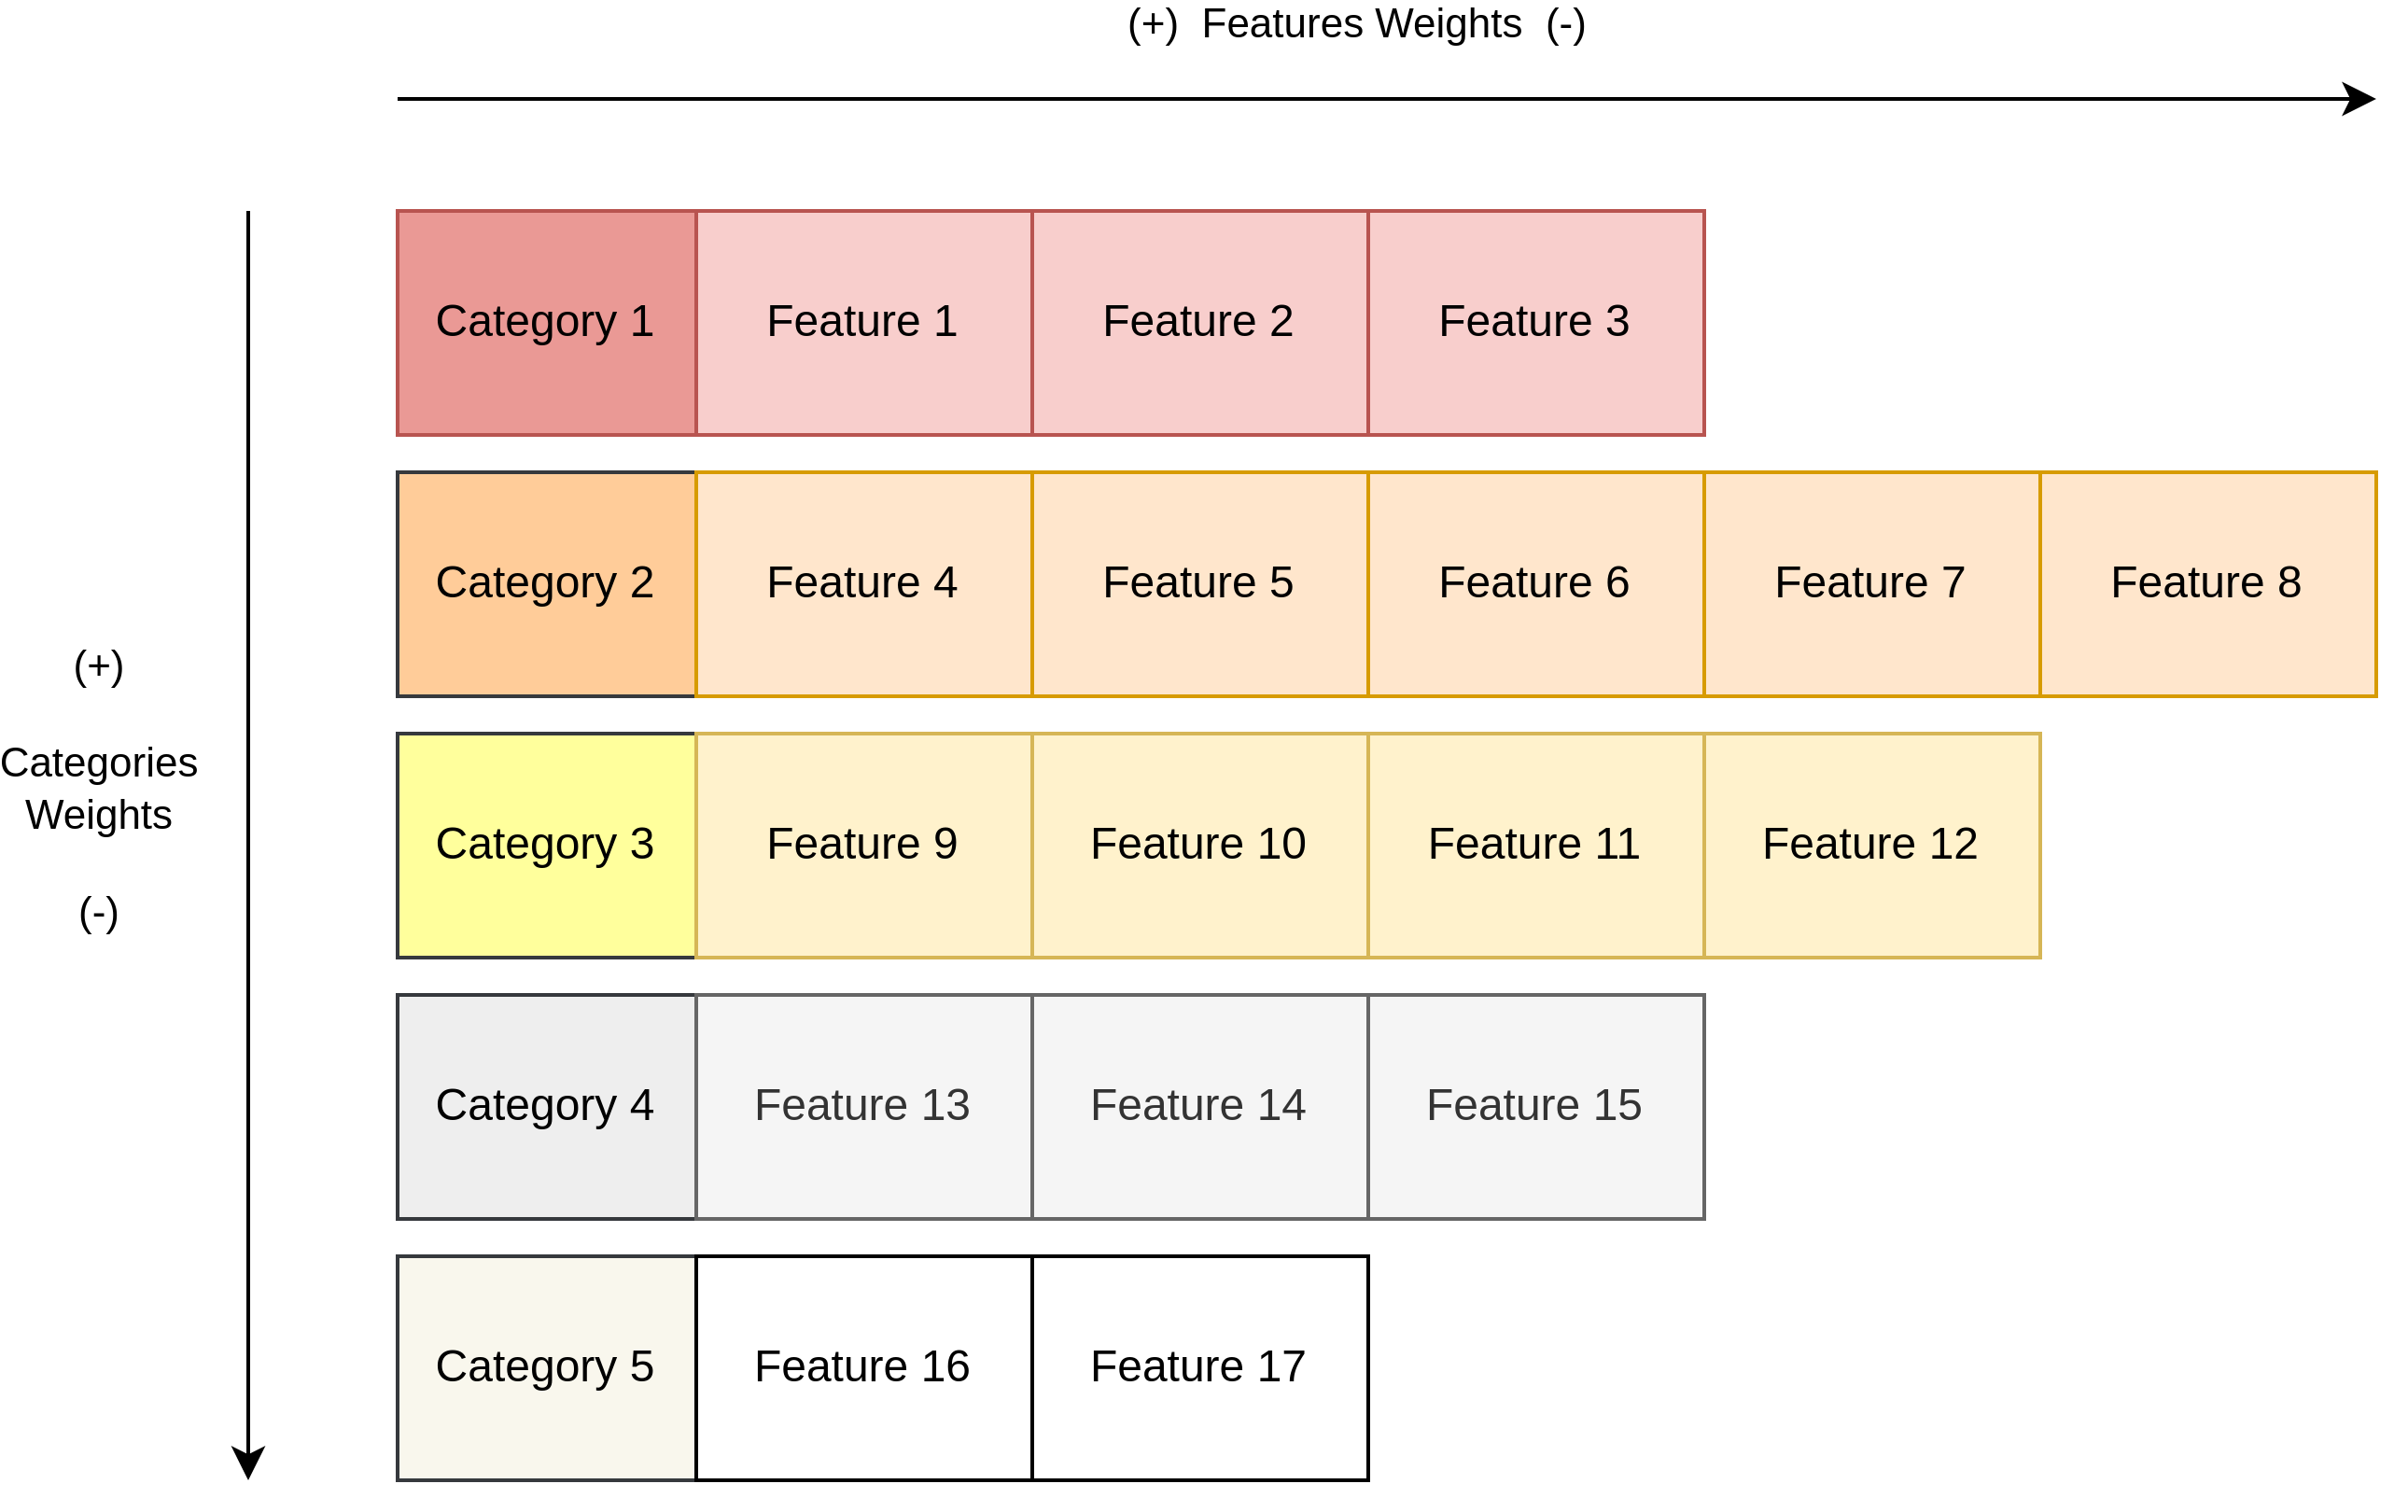
\includegraphics[width=14cm]{Figures/indexing_positions_1_2.png}
    \caption{Category and feature weights.}
    \label{CategoriesFeaturesWeights}
\end{figure}

El resultado de este proceso es una transformación de datos inicialmente tabulares en una matriz $n \times m$, donde $n$ es el número de categorías disponibles en los datos y $m$ es el número de máximo de características que contienen las categorías. Estas matrices están conformadas siguiendo que las variables más importantes para los datos se encuentran en las posiciones centrales, como se muestra en la Figura \ref{MatrixIndexes}.


\begin{figure}[H]
    \centering
    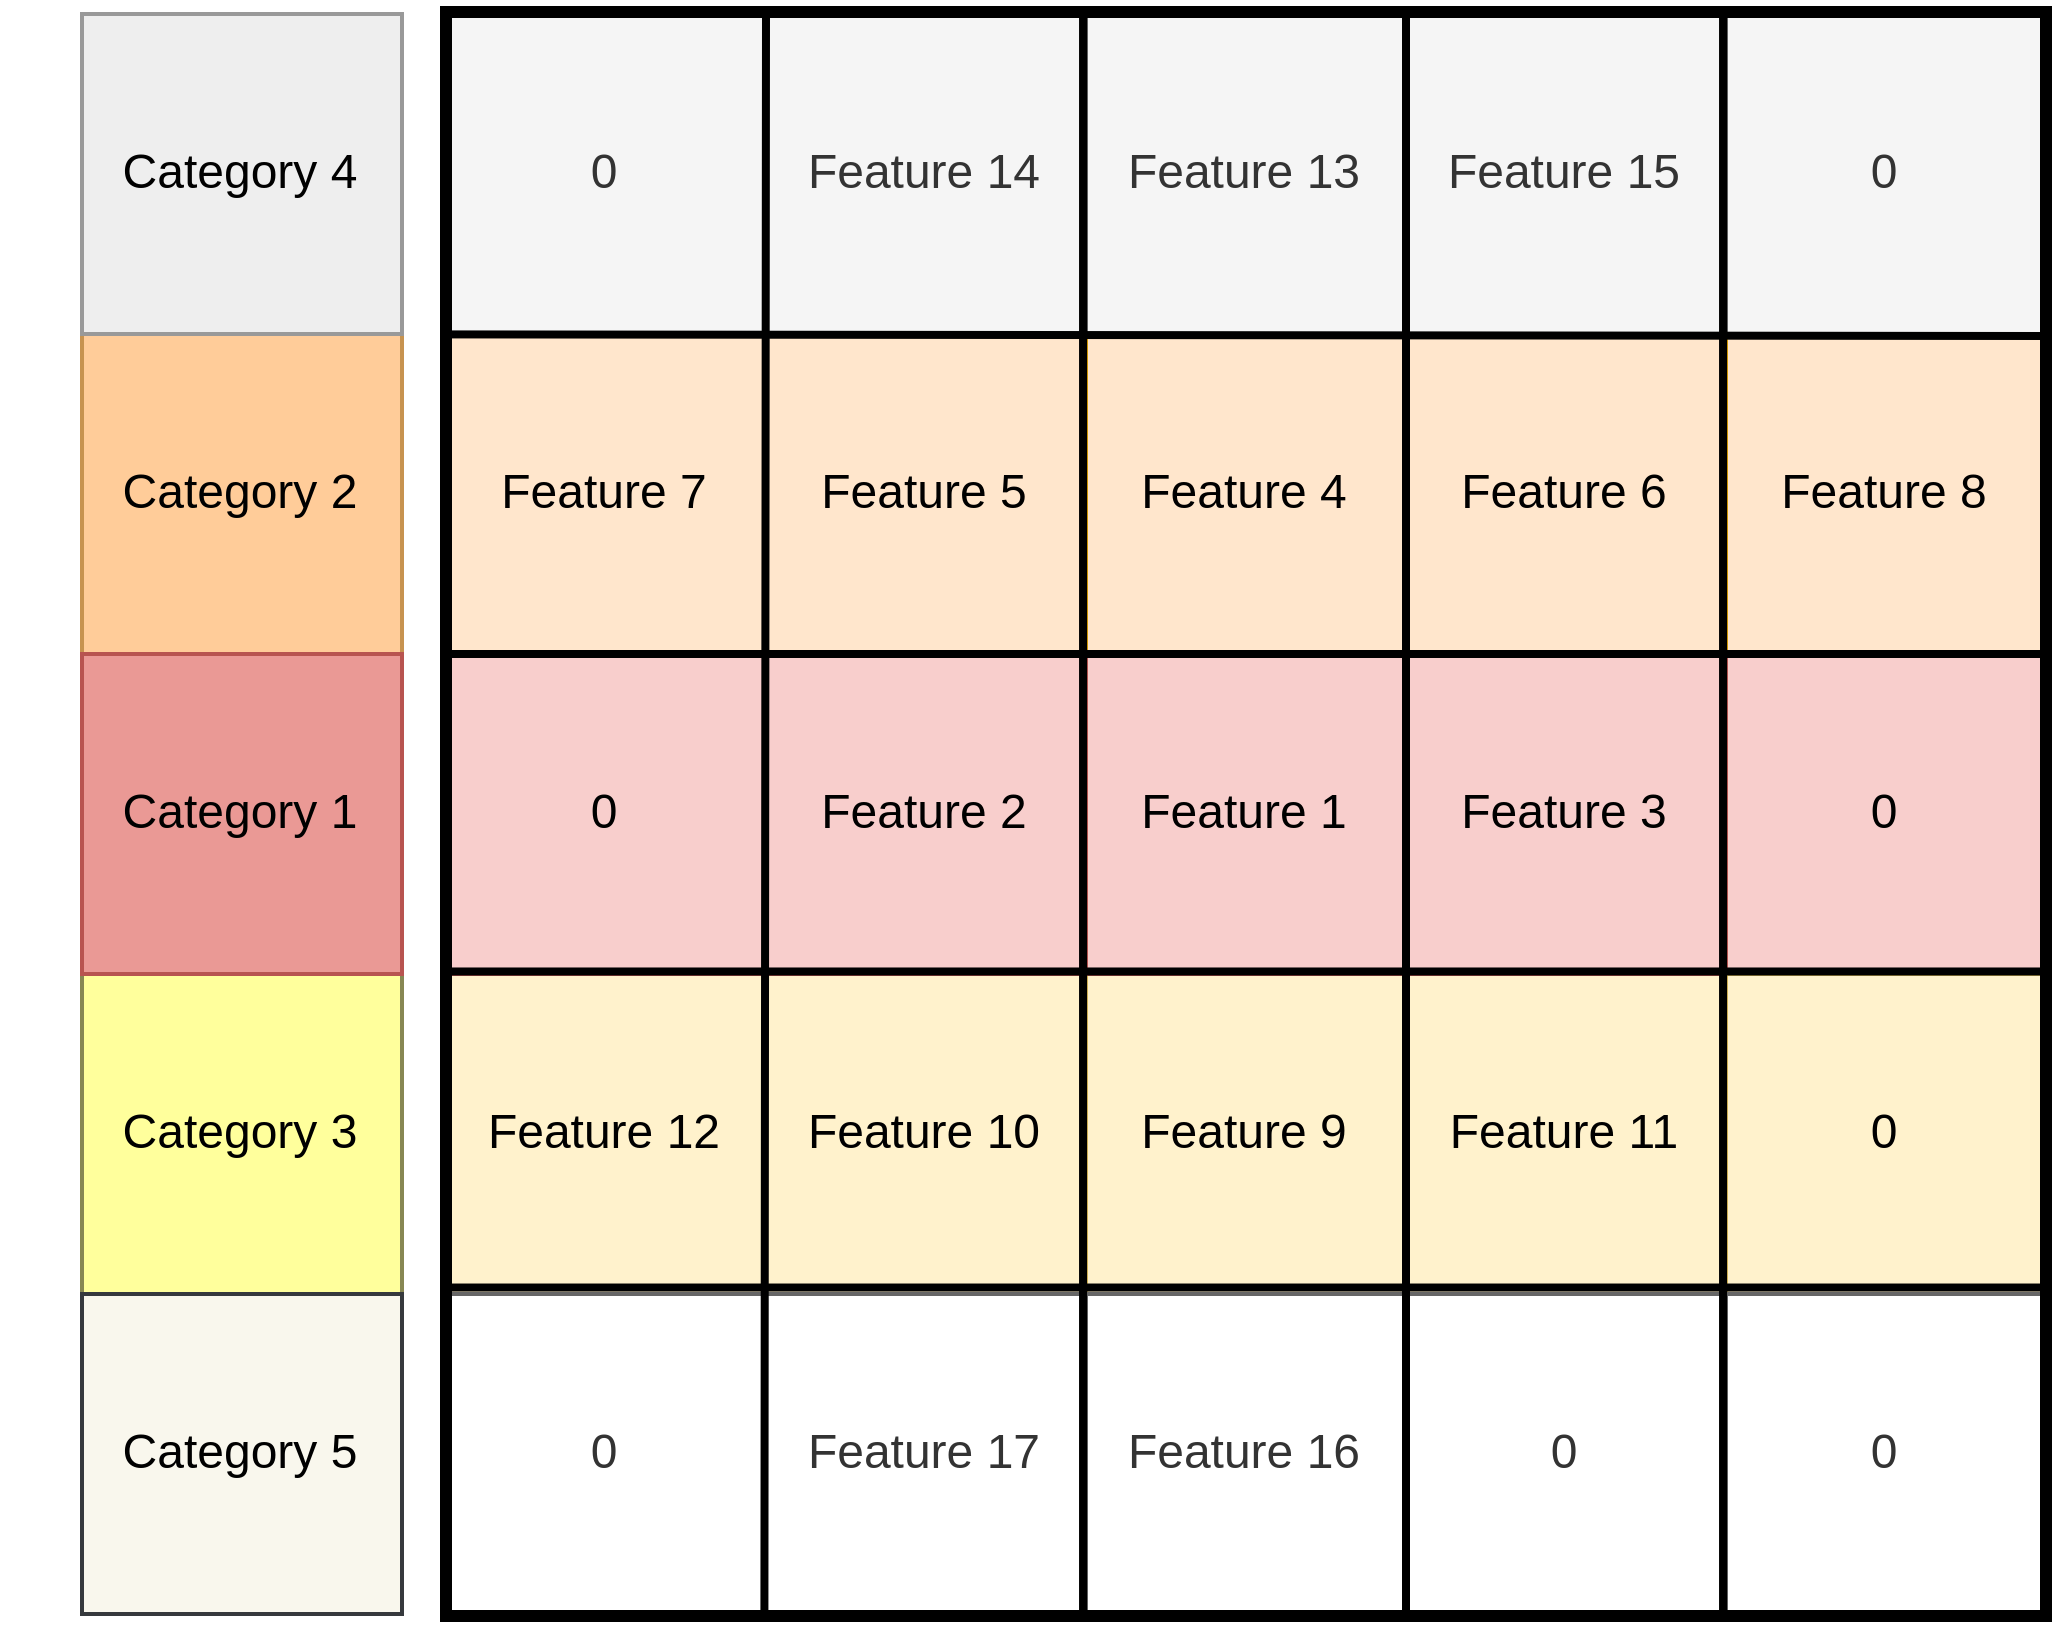
\includegraphics[width=10cm]{Figures/indexing_positions_2.png}
    \caption{Categories and feature positions.}
    \label{MatrixIndexes}
\end{figure}

En la Figura \ref{MatrixConstruction} se muestra un ejemplo del procedimiento 

\begin{figure}[H]
    \centering
    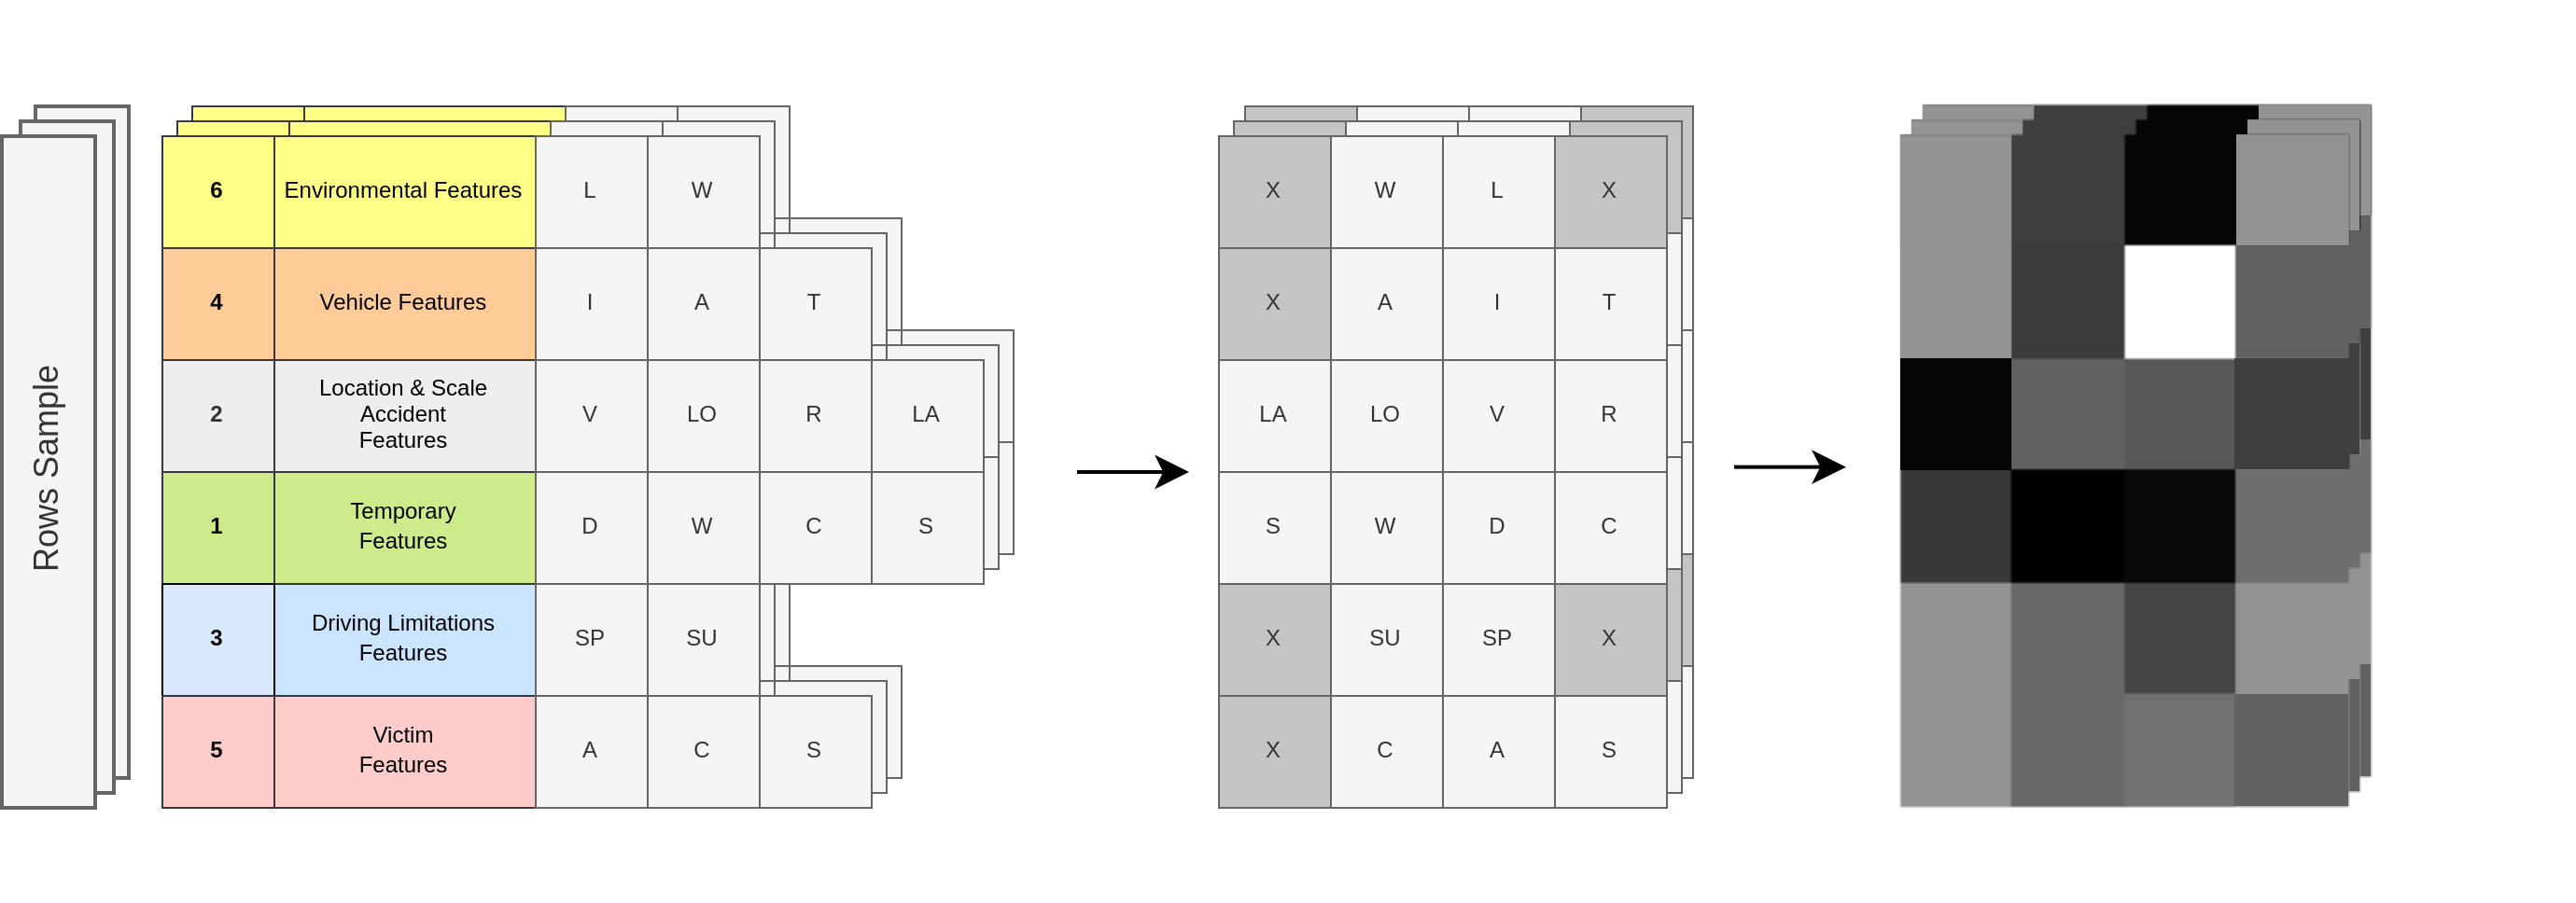
\includegraphics[width=17cm]{Figures/Matrix Construction_2.png}
    \caption{Assignment process of features to matrix positions. Categories are arranged based on their weight and assigned to rows of the matrix; subsequently, features within their respective categories are positioned.}
    \label{MatrixConstruction}
\end{figure}

\subsection{Diseño del modelo}

El nuevo modelo propuesto presenta una arquitectura de cuatro capas convolucionales de dos dimensiones cada una, con un tamaño de kernel de $3 \times 3$ y una función de activación ReLU. A la salida de cada capa convolucional se aplica un proceso de Batch Normalization.

La primera capa convolucional de la red consta de 64 kernels, la segunda de $512$, la tercera de $128$ y la cuarta de $256$. Estos kernels contienen los pesos que se entrenan durante la fase de ajuste del modelo a partir de la salida conocida de los datos etiquetados, aprendiendo qué multiplicaciones en los datos minimizan la función de pérdida definida de la red (entropía cruzada binaria) gracias al proceso de retropropagación. La salida de cada capa convolucional son los mapas de características, que son el resultado de aplicar la multiplicación de estos filtros a su entrada. El paso, o número de unidades que avanzan los kernels para un mapa de características, es 1. También se aplica relleno en las convoluciones, es decir, si la multiplicación del kernel excede los límites de la matriz, se agregarán ceros a estos límites para realizar la convolución. Los mapas de características resultantes de la última capa pasan a través de una capa de aplanamiento, que transforma los datos a una sola dimensión una vez que han finalizado las convoluciones. Cada uno de estos datos aplanados está interconectado con los $256$ nodos definidos de la capa densa (Fully Connected Network). Finalmente, la capa densa está conectada a una capa densa final con la función de activación Softmax, que da la probabilidad de que cada nueva muestra pertenezca a una de las dos clases. En la figura \ref{CNN2DArchitecture} se puede observar, a modo de diagrama, la intuición de la arquitectura de la red.


\begin{figure}[H]
    \centering
    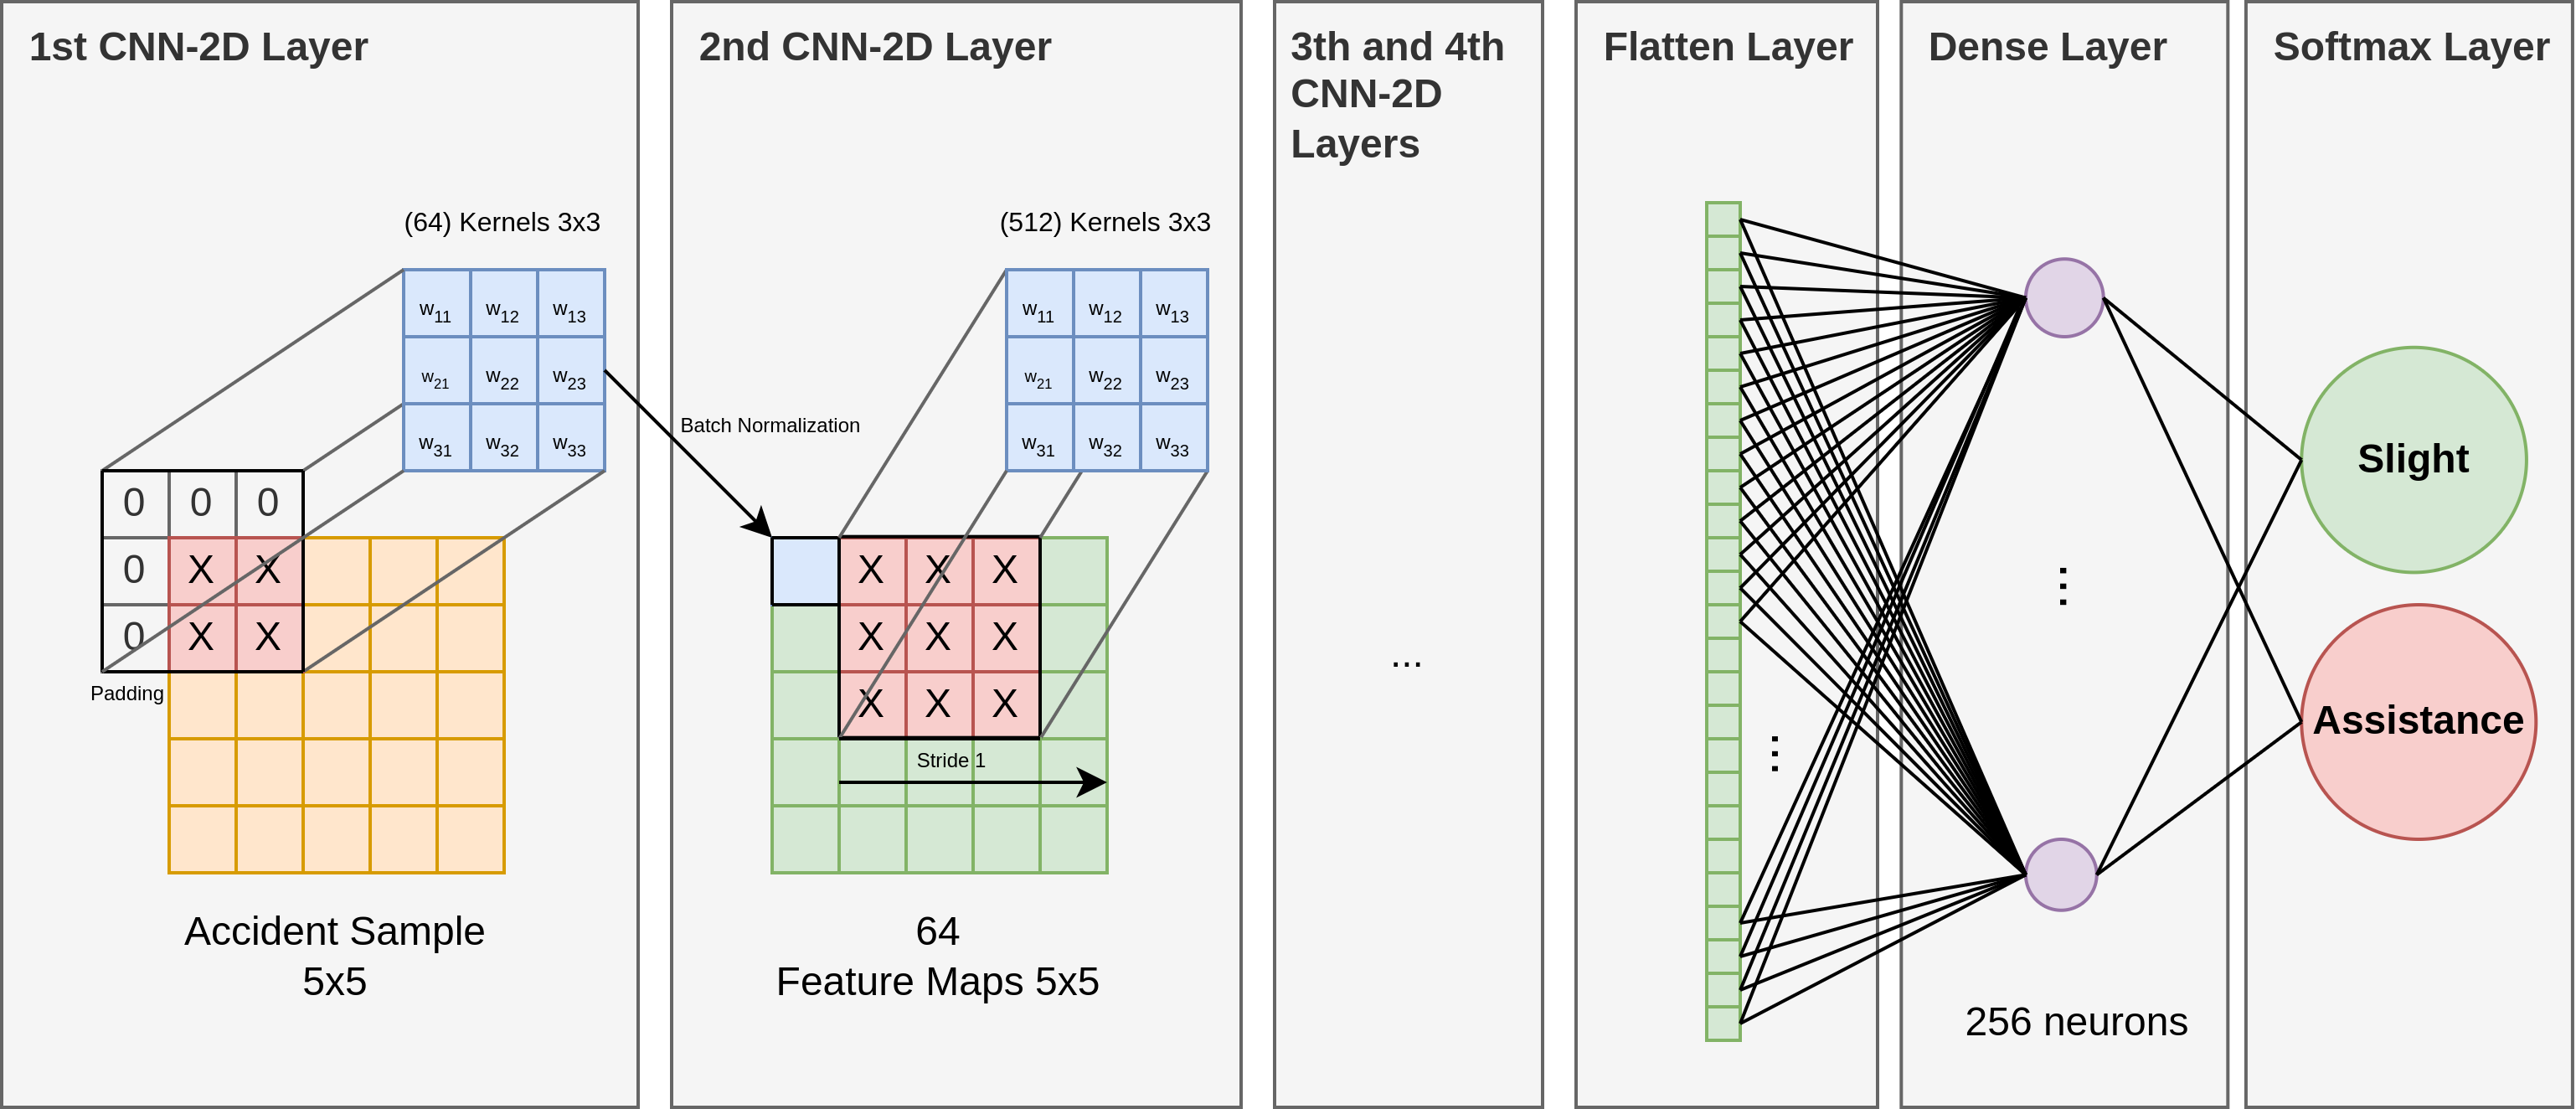
\includegraphics[width=15cm]{Figures/SIMPLE.png}
    \caption{Proposed CNN-2D architecture summary.}
    \label{CNN2DArchitecture}
\end{figure}

\section{Evaluación del modelo: Eficiencia y Robustez}


\chapter{Experimentos y resultados}



\section{Resultados preliminares - Prototipo}

\underline{Aquí pones los resultados del paper 1}


\textcolor{red}{Explicar el artículo, indicando los enfoques tomados y las decisiones...}

Como etapa previa al modelo final, y a modo de prototipo, se construyó un modelo primigenio que fue evolucionando hasta llegar a la metodología final expuesta en esta tesis. Sobre este primer modelo, se fueron aplicando modificaciones y mejoras en base al análisis de los resultados obtenidos durante su ciclo de vida hasta llegar a la "versión definitiva" de esta tesis. A modo de justificar las decisiones y criterios expuestos en este documento, en esta sección se expondrá el procedimiento inicial, los análisis de resultados y las mejoras propuestas que dan lugar a la versión final.


%Como etapa previa a y con objetivo de justificar las decisiones y los criterios expuestos en esta tesis en los apartados anteriores, se construyó un primer prototipo  

Este prototipo se presentó en el artículo \cite{PEREZSALA2023113245}, y se construyó con el objetivo de predecir la gravedad de los accidentes de tráfico en la ciudad de Madrid, dividiendo la severidad de los accidentes en tres clases (Leves, Severos y Fatales). 


\underline{Descripción de datos}

Los datos originales presentados en este prototipo pertenecían a la ciudad de Madrid, que describían ocurrencias de accidentes de tráfico a lo largo de toda la ciudad a través de 18 características entre los años 2019 y 2022, con un total de 60.966 registros. La variable a predecir representaba la lesividad que había sufrido la víctima implicada en el accidente, y que en el conjunto de datos era considerada en 7 clases, que se interpretaron finalmente como 3:


\begin{enumerate}
	\item Leve: esto varía desde aquellos que no han sido heridos hasta aquellos que han necesitado ser admitidos en un hospital por no más de 24 horas. La cuantificación numérica es:
	\begin{itemize}
		\item Atención de emergencia sin posterior admisión hospitalaria: $1$.
		\item Admisión hospitalaria menor o igual a 24 horas: $2$.
		\item Atención médica ambulatoria después del accidente: $5$.
		\item Atención médica solo en el lugar del accidente: $6$.
		\item Sin atención médica: $7$.
	\end{itemize}
	\item Grave: aquellos involucrados que han requerido hospitalización por más de 24 horas. En este caso, la cuantificación numérica es:
	\begin{itemize}
		\item Hospitalización por más de $24$ horas: $3$.
	\end{itemize}
	\item Fatal: fatalidades dentro de las $24$ horas posteriores al accidente. La asignación numérica para este campo es:
	\begin{itemize}
		\item Fallecido dentro de las $24$ horas: $4$.
	\end{itemize}
\end{enumerate}

\underline{Limpieza}
	
El resto de características describían información del accidente, como el lugar en el que se había producido, información del vehículo o información sobre la víctima. No obstante, existían conjuntos de variables que presentaban correlaciones entre sí (algo que afecta negativamente al rendimiento de los modelos) y contenían valores atípicos o nulos. Es por esto por lo que en primer lugar era necesario aplicar un proceso de análisis para evaluar el alcance y la calidad los datos aplicar que comenzaba por un proceso de limpieza que pretendía disponer de un dataset refinado e interpretable por distintos métodos, por lo que se eliminaron los registros con valores atípicos y aquellos que presentaban valores nulos, resultando un dataset final con 54.364 registros, un 10.82\% de pérdida de información respecto al original.


\underline{Discretización}

\textbf{Luis: } Me parece raro presentar los datos ya filtrados y luego después de la tabla explicar que son los resultantes del proceso de eliminación en función del 0,44 de correlación).\\


En la figura \ref{Datadescription} se muestra la descripción detallada de cada variable en esta etapa de la metodología.

\textbf{Luis: TODO} Esta tabla está copiada y pegada del paper 1).\\
%%%%%%%%%%%%%%%%%%%%%%%%%%%%%%%%%%%%%%%%%%%%%%%%%%%%%%%%%%%%%%%%%%%%%%%%%%%%%%%%%
\begin{table}[H]
	\begin{center}
		\begin{tabular}{|p{3cm}|p{12cm}|}
			\hline
			\textbf{Atributo} & \textbf{Descripción} \\ \hline \hline
			ID de Incidente  & Identificador del incidente, si varios registros tienen el mismo número de archivo, se consideran el mismo accidente y cada registro representa a cada una de las personas involucradas en él (conductor, pasajero o peatón)  \\ \hline
			Fecha  & Día, mes y año en que ocurrió el incidente \\ \hline
			Hora  & Hora y minutos en que ocurrió el incidente \\ \hline
			Tipo de Carretera & Tipo de carretera donde ocurrió el incidente \\ \hline
			Nombre & Nombre de la calle donde ocurrió el incidente \\ \hline
			Número de Calle & Número de la calle donde ocurrió el incidente  \\ \hline
			Distrito & Nombre del distrito donde ocurrió el incidente \\ \hline
			Tipo de Accidente  & Puede ser: doble colisión, colisión múltiple, alcance, colisión con un obstáculo, atropello, vuelco, caída u otras causas \\ \hline
			Condiciones climáticas  & Condiciones climáticas en el momento del incidente \\ \hline
			Vehículo  & Clasificación según tipos de vehículos \\ \hline
			Persona  & Rol de la persona involucrada: conductor, pasajero o peatón \\ \hline
			Edad  & Rango de edad de la persona involucrada \\ \hline
			Género  & Mujer u hombre \\ \hline
			\textbf{Severidad}  & Consecuencias físicas de la persona involucrada, si han necesitado atención médica, si han sido hospitalizados o si han sido fatales \\ \hline
			X   & Coordenada X - UTM \\ \hline
			Y   & Coordenada Y - UTM \\ \hline
			Alcohol & Si la persona involucrada ha dado positivo en alcohol (S o N) \\ \hline
			Drogas & Si la persona involucrada ha dado positivo en drogas (S o N) \\ \hline \hline
		\end{tabular}
	\end{center}
	\caption{Variables del conjunto de datos y sus descripciones.}
	\label{Datadescription}
\end{table}
%%%%%%%%%%%%%%%%%%%%%%%%%%%%%%%%%%%%%%%%%%%%%%%%%%%%%%%%%%%%%%%%%%%%%%%%%%%%%%%%%

Una vez se disponen de unos datos refinados, era necesario transformarlos para hacerlos interpretables por los modelos. Este proceso se hizo mediante la asignación de valores numéricos a cada una de las variables cualitativas del dataset, en función de la fuerza del significado de los valores de cada característica, en la Figura \ref{1stPaperTransformacionDatosTabla} se muestra la discretización de las variables seleccionadas de este conjunto de datos.

%%%%%%%%%%%%%%%%%%%%%%%%%%%%%%%%%%%%%%%%%%%%%%%%%%%%%%%%%%%%%%%%%%%%%%%%%%%%%%%%%
\begin{table}[H]
	\centering
	\renewcommand{\arraystretch}{1.4}
	\scriptsize
	\begin{minipage}{0.4\textwidth}
		\begin{tabular}{|l|l|}
			\hline
			\textbf{Características} & \textbf{Tipificación}\\
			\hline
			\multirow{\textbf{Gravedad}}  & 0: Leve (\textit{1, 2, 5, 6, 7})\\
			& 1: Grave (\textit{3})\\
			& 2: Fatal (\textit{4})\\
			\hline
			\multirow{Tiempo}     & 1: Noche (\textit{6 PM - 6 AM})\\
			& 2: Día (\textit{6 AM - 6 PM})\\
			\hline
			\multirow{Distrito}   & Basado en orden de aparición\\
			\hline
			\multirow{X}   & Posición de Coordenada UTM X\\
			\hline
			\multirow{Y}   & Posición de Coordenada UTM Y\\
			\hline
			\multirow{Tipo de Accidente} & 1: Colisión frontal - tamaño\\
			& 2: Colisión trasera\\
			& 3: Choque lateral\\
			& 4: Colisión con obstáculo fijo\\
			& 5: Choque en cadena\\
			& 6: Atropello a peatón\\
			& 7: Colisión frontal\\
			& 8: Otro\\
			& 9: Salida de la carretera\\
			& 10: Vuelco de vehículo\\
			& 11: Atropello a animal\\
			& 12: Caída\\
			\hline
			\multirow{Tipo de Camino}     & 1: Estacionamiento \\
			& 2: Aeropuerto\\
			& 3: Parque\\
			& 4: Túnel\\
			& 5: Zona industrial\\
			& 6: Pista\\
			& 7: Rotonda\\
			& 8: Glorieta\\
			& 9: Puerta\\
			\hline
		\end{tabular}
	\end{minipage} \hspace{10mm}
	\begin{minipage}{0.4\textwidth}
		\begin{tabular}{|l|l|}
			\hline
			\textbf{Característica} & \textbf{Tipificación}\\
			\hline
			\multirow{Tipo de Camino}     
			& 10: Puente\\
			& 11: Plaza\\
			& 12: Bulevar\\
			& 13: Cruce\\
			& 14: Calzada\\
			& 15: Carretera\\
			& 16: Avenida\\
			& 17: Autopista\\
			& 18: Calle\\
			\hline
			\multirow{Condiciones Meteorológicas}   & 1: Soleado\\
			& 2: Nublado\\
			& 3: Lluvia ligera\\
			& 4: Lluvia intensa\\
			& 5: Granizo\\
			& 6: Nevando\\
			& 7: Desconocido\\
			\hline
			\multirow{Vehículo}  & Basado en orden de aparición\\
			\hline
			\multirow{Persona}   & 1: Conductor\\
			& 2: Pasajero\\
			& 3: Peatón\\
			\hline
			\multirow{Edad}      & 1: Menos de 18 años\\
			& 2: De 18 a 25 años\\
			& 3: De 25 a 65 años\\
			& 4: Más de 65 años\\
			& 5: Desconocida\\
			\hline
			\multirow{Género}   & 1: Masculino\\
			& 2: Femenino\\
			& 3: Desconocido\\
			\hline
			\multirow{Alcohol o Drogas} & 1: Sí\\
			& 2: No\\
			\hline
		\end{tabular}
	\end{minipage}
	\caption{Asignación numérica de las variables del conjunto de datos.}
	\label{1stPaperTransformacionDatosTabla}
\end{table}
	
%%%%%%%%%%%%%%%%%%%%%%%%%%%%%%%%%%%%%%%%%%%%%%%%%%%%%%%%%%%%%%%%%%%%%%%%%%%%%%%%%

Para entrenar un modelo de Inteligencia Artificial es necesario analizar la dependencia entre cada par de variables, por esto se analizó la relación entre variables mediante una matriz de correlación. Estas matrices muestran la fuerza mediante la que variable es dependiente respecto al resto de las demás, los coeficientes de correlación varían entre -1 y 1, indicando la magnitud y dirección de esta dependencia. Una vez analizadas estas métricas, se aplicó un límite de correlación entre variables del $\pm 0.44$, lo que quiere decir que aquellas que presentasen un índice que superase este valor se verían excluidas del dataset. En la figura \ref{CorrelationMatrix} se muestra la matriz de correlación resultante tras eliminar las características que superasen este umbral de dependencia entre sí.


 \begin{figure}[H]
	\centering
	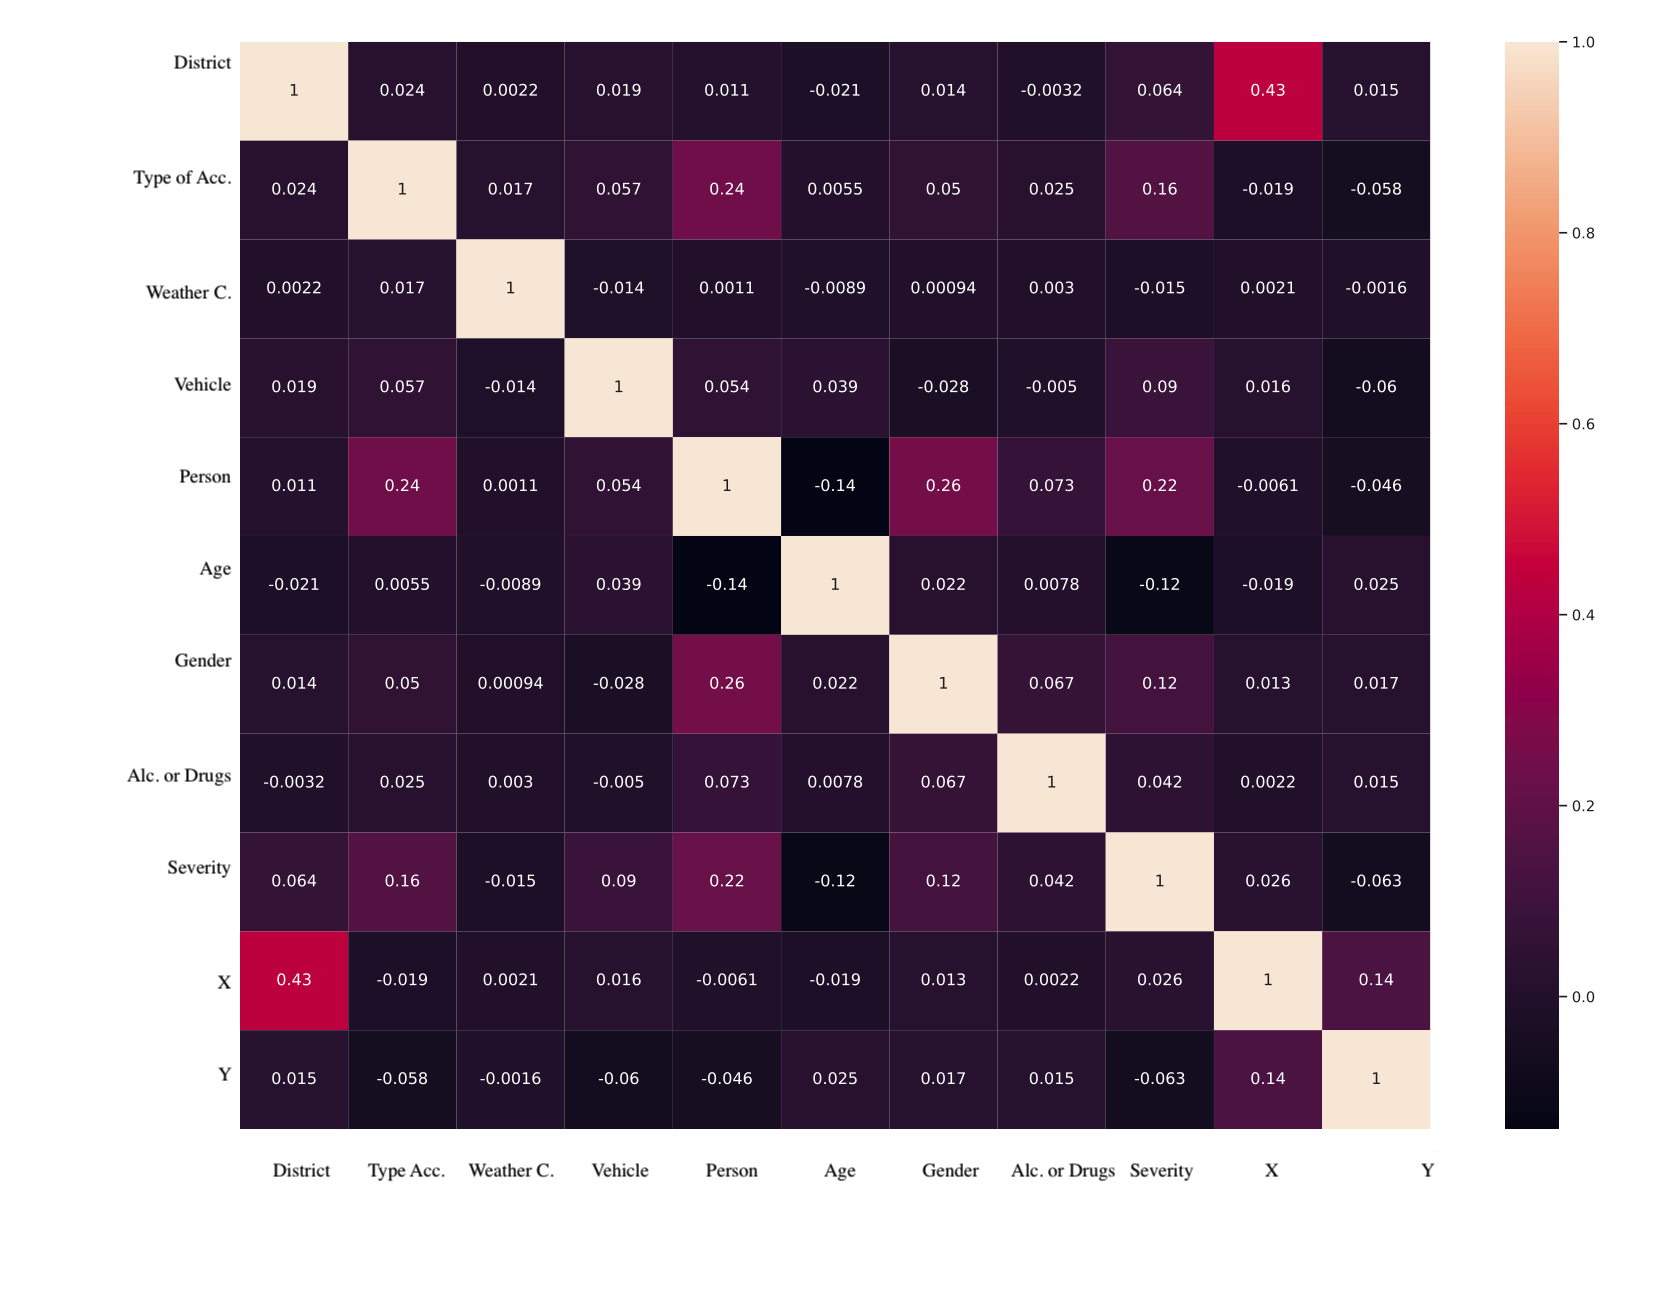
\includegraphics[width=12cm]{Figures/1stPaper/CorrelationMatrix.png}
	\caption{Correlation matrix between the dataset variables.}
	\label{CorrelationMatrix}
\end{figure}



\underline{Resampling}

Una vez aplicado el proceso de limpieza de datos y elección de características del dataset, se analizó la distribución final de los datos en base a la clase a predecir, la severidad de accidente. Atendiendo a los registros resultantes (Leve, Grave y Fatal), se puede observar que el conjunto de datos está claramente desbalanceado. Se disponían de $53,009$ accidentes leves, $1,271$ graves y $84$ fatales. Esto se convierte en un problema para los modelos de clasificación, ya que tienden a predecir las muestras como pertenecientes a la mayoría del conjunto de pruebas. Para paliar este problema se aplicó la técnica de remuestreo Borderline SMOTE-II para generar más muestras de accidentes pertenecientes a clases minoritarias (Grave y Fatal), evitando que el modelo se sobreajuste. Una vez aplicado el algoritmo, se obtienen $42,508$ muestras de cada una de las clases de accidentes, es decir, un total de $127,524$ registros.


\underline{Normalización}

En la Figura \ref{TFM_NormalizationExample} se muestra un ejemplo de la aplicación de la normalización de datos en base a la técnica Z-Score, donde en la primera Tabla \ref{TFM_NormalizationExample:MuestraTipificada} se observa un registro de datos discretizado del dataset y el la Figura \ref{TFM_NormalizationExample:MuestraNormalizada} se observa esta misma muestra tras haber aplicado el proceso de normalización. Este proceso se aplica para cada una de las muestras de tal forma que la dimensión de los datos estén bajo la misma magnitud, para poder ser eficientemente interpretables por los modelos.


\begin{figure}[H]
	\scriptsize
	\centering
	\renewcommand{\arraystretch}{1.4}
	
	\captionsetup{singlelinecheck = false, format= hang, justification=raggedright, font=footnotesize, labelsep=space}
	
	\begin{c}
		\centering
		\csvautotabular{Figures/TFM/fatal_original.csv}
		
		\captionsetup{singlelinecheck = false, format= hang, justification=centering, font=footnotesize, labelsep=space}
		
		\caption{Muestra de accidente tipificada.}
		\label{TFM_NormalizationExample:MuestraTipificada}
	\end{c}
	\begin{c}
		\centering
		\csvautotabular{Figures/TFM/fatal_normalized.csv}
		
		\captionsetup{singlelinecheck = false, format= hang, justification=centering, font=footnotesize, labelsep=space}
		
		\caption{Muestra de accidente tipificada.}
		\label{TFM_NormalizationExample:MuestraNormalizada}
	\end{c}
	\caption{Ejemplo de normalización de una muestra del dataset.}
	\label{TFM_NormalizationExample}
\end{figure}%


Una vez se disponen de los datos normalizados, estos ya se encuentran en las mismas magnitudes y por tanto pueden ser utilizados para el entrenamiento de cualquier modelo predictivo.

\underline{División Train-Val-Test}

El siguiente paso, necesario en cualquier procedimiento de entrenamiento de un modelo predictivo, fue la división entre datos de entrenamiento y datos de validación. Esta división se realiza asignando un 80\% de los datos del dataset para asignarlos al entrenamiento y un 20\% a validación o test.


\underline{Categorización}

Como se ha comentado en la sección de metodología, las redes neuronales convolucionales (CNN) aprenden patrones utilizando matrices como datos de entrada, y cuando se trata de datos tabulares, es necesario transformar estos datos a datos matriciales.

Para lograr este objetivo, uno de los requisitos de esta transformación era asignar cada característica a una categoría del dataset. Sobre este conjunto de datos, las variables eran asignadas a 5 categorías: Características del accidente, Condiciones de la carretera, Condiciones meteorológicas, Características del vehículo y Características del conductor. En la Tabla \ref{JC} se observa la categorización de cada característica a una categoría en función del concepto que describan.

\begin{table}[H]
	\centering

		\begin{tabular}{ |c|c| }
			\hline
			\textbf{Categoría} & \textbf{Característica} \\
			\hline
			\hline
			\multirow{5}{*}{Accidente} & X \\
									   & Y \\
									   & Hora \\
									   & Tipo de accidente \\
									   & Severidad \\
			\hline
			\hline
			\multirow{2}{*}{Carretera} & Tipo de carretera \\
									   & Distrito \\
			\hline
			\hline
			Clima & Condiciones climáticas \\
			\hline
			\hline
			Vehículo & Vehículo \\
			\hline
			\hline
			\multirow{4}{*}{Conductor} & Persona \\
									   & Género \\
									   & Edad \\
									   & Alcohol o Drogas \\
			\hline
			\hline
		\end{tabular}

	\caption{Clasificación de las Características (variables del conjunto de datos) en Categorías.}
	\label{JC}
\end{table}


\underline{Algoritmo Genético}

En este punto, se analiza la optimización de los hiperparámetros del algoritmo de Boosting mediante un algoritmo genético. La figura \ref{EvolucionHiperparametrosImage} muestra la evolución de  los tres hiperparámetros a lo largo de las generaciones. Como se puede observar, los hiperparámetros toman distintos valores en función del mejor individuo evaluado en la población en cada etapa, estos hiperparámetros convergen aproximadamente en la iteración $42$, donde no se observan modificaciones a partir de esta generación.

 \begin{figure}[H]
	     \centering
	     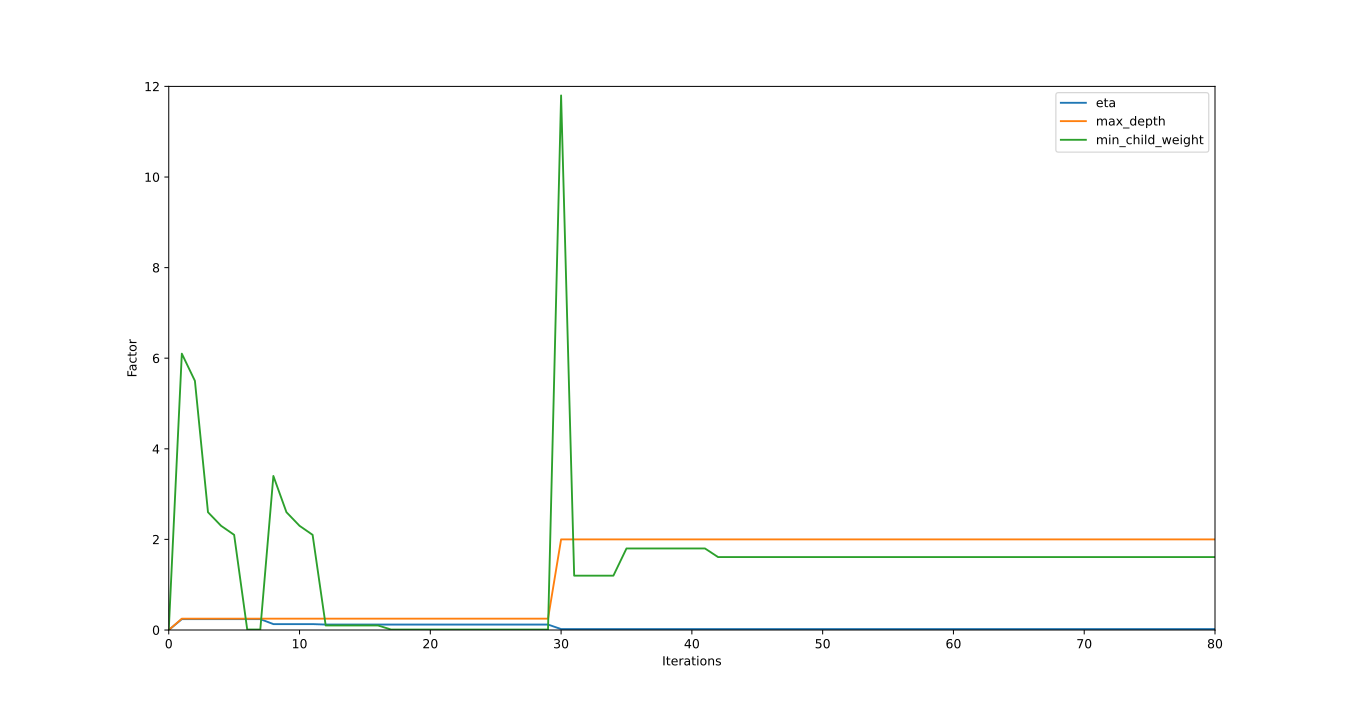
\includegraphics[width=14cm]{Figures/1stPaper/EvolutionH.png}
	     \caption{Evolution of hyperparameters throughout the iterations.}
	     \label{EvolucionHiperparametrosImage}
 \end{figure}


En la tabla \ref{BestGASolutionTable} se observa el valor tomado el mejor individuo entre las distintas generaciones para cada uno de los hiperparámetros del XGBoost, esta será la configuración con la que se entrenará el algoritmo para obtener el peso de las características del dataset.

%%%%%%%%%%%%%%%%%%%%%%%%%%%%%%%%%%%%%%%%%%%%%%%%%%%%%%%%%%%%%%%%%%%%%%%%%%%%%%%%%
\begin{table}[h]
	\centering
	\begin{tabular}{ |l|c| } 
		\hline
		\textbf{Hyperparameters} & \textbf{Value}\\
		\hline
		Max deep & 2 \\
		Minimum weight of children & 1.6 \\ 
		ETA & 0.007 \\
		Gamma & 0.3 \\
		Alpha & 0 \\
		Lambda & 1 \\
		\hline
	\end{tabular}
	\caption{Optimized values of the parameters after applying the genetic algorithm.}
	\label{BestGASolutionTable}
\end{table}
%%%%%%%%%%%%%%%%%%%%%%%%%%%%%%%%%%%%%%%%%%%%%%%%%%%%%%%%%%%%%%%%%%%%%%%%%%%%%%%%%

%\underline{Pesos de categorías}

En la Tabla \ref{1stPaperWeightsFinalCharacteristics} se observa el peso asignado a cada una de las características individuales resultante del entrenamiento XGBoost con los hiperparámetros optimizados. En la columna "Categoría de Peso" se observa el peso de cada categoría, que es la suma del peso de las características individuales que las componen.

%%%%%%%%%%%%%%%%%%%%%%%%%%%%%%%%%%%%%%%%%%%%%%%%%%%%%%%%%%%%%%%%%%%%%%%%%%%%%%%%%
\begin{table}[H]
	\centering
	\begin{tabular}{ |c|c|c|c| }
		\hline
		\textbf{Categoría} & \textbf{Categoría de Peso} & \textbf{Característica} & \textbf{Peso de la Característica}\\
		\hline
		\hline
		\multirow{5}{*}{Accidente}   & \multirow{5}{*}{0.299} & Coordenada X & 0.071\\
		&  & Coordenada Y  & 0.066\\
		&  & Hora & 0.055\\
		&  & Tipo de accidente  & 0.051\\
		&  & Severidad & 0.057\\
		\hline
		\hline
		\multirow{2}{*}{Carretera} & \multirow{2}{*}{0.187} & Distrito  & 0.059\\      
		&  & Tipo de Carretera & 0.127\\
		\hline
		\hline
		\multirow{1}{*}{Clima}  & \multirow{1}{*}{0.050}  & Condiciones Climáticas  & 0.050\\
		\hline
		\hline
		\multirow{1}{*}{Vehículo}  & \multirow{1}{*}{0.070} & Vehículo  & 0.070\\
		\hline
		\hline
		\multirow{4}{*}{Conductor}   & \multirow{4}{*}{0.394} & Persona & 0.177\\
		&      & Género      & 0.111\\
		&      & Edad      & 0.050\\
		&      & Alcohol o Drogas  & 0.056\\
		\hline
		\hline
	\end{tabular}
	\caption{Ejemplo con los pesos de todas las características estudiadas, así como los pesos de las cinco categorías.}
	\label{1stPaperWeightsFinalCharacteristics}
\end{table}

%%%%%%%%%%%%%%%%%%%%%%%%%%%%%%%%%%%%%%%%%%%%%%%%%%%%%%%%%%%%%%%%%%%%%%%%%%%%%%%%%

\underline{Construcción de matrices}

Una vez se disponían de las características y categorías evaluadas, se aplicaba el proceso de asignación de posiciones de cada característica a una coordenadas dentro de la matriz, aplicando el algoritmo de construcción de matrices.

En la Figura \ref{ProcesoMatriz:Array} se observa un ejemplo de un registro transformado a formato matricial una vez aplicado el algoritmo de construcción haciendo uso de la importancia de las características de la tabla \ref{1stPaperWeightsFinalCharacteristics}, y en \ref{ProcesoMatriz:VisualizacionDeMatriz} se observa la representación en imagen de dicha matriz.

%%%%%%%%%%%%%%%%%%%%%%%%%%%%%%%%%%%%%%%%%%%%%%%%%%%%%%%%%%%%%%%%%%%%%%%%%%%%%%%%%%
%\begin{table}[H]
%	\centering
%	\begin{tabular}{|ccccc|}
%		%\hline
%		0.0   & 0.0   & 0.05  & 0.0   & 0.0 \\
%		0.0   & 0.059 & 0.128 & 0.0   & 0.0 \\ 
%		0.050 & 0.111 & 0.177 & 0.056 & 0.0 \\
%		0.055 & 0.066 & 0.071 & 0.057 & 0.051 \\
%		0.0   & 0.0   & 0.070 & 0.0   & 0.0 \\
%		%\hline
%	\end{tabular}
%	\caption{A specific accident matrix.}
%	\label{1stPaperFeaturesNormalizationExample}
%\end{table}
%%%%%%%%%%%%%%%%%%%%%%%%%%%%%%%%%%%%%%%%%%%%%%%%%%%%%%%%%%%%%%%%%%%%%%%%%%%%%%%%%%

\begin{figure}[H]\ContinuedFloat
	\scriptsize
	\centering
	\vskip\baselineskip
	\begin{subtable}
		\centering
		\renewcommand{\arraystretch}{1.5}
		
		\csvreader[
		tabular = |c|c|c|c|c|,
		table head = \hline,
		table foot = \hline
		]{Figures/TFM/fatal_matrix.csv}%
		{0=\cero, 1=\one, 2=\two, 3=\three, 4=\four}{%
			\cero & \one & \two & \three &  \four
		}
		\captionsetup{singlelinecheck = false, format= hang, justification=centering, font=footnotesize, labelsep=space}
		\caption{Matriz resultante tras la transformación de un registro a formato matricial.}
		\label{ProcesoMatriz:Array}
	\end{subtable}
	\hspace{5em}
	\begin{subfigure}
		\centering
		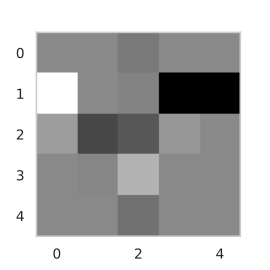
\includegraphics[scale=0.5]{Figures/TFM/accidente_fatal.png}
		\captionsetup{singlelinecheck = false, format= hang, justification=centering, font=footnotesize, labelsep=space}
		\caption{Imagen de las características.}
		\label{ProcesoMatriz:VisualizacionDeMatriz}
	\end{subfigure}
	\caption{Ejemplo de representación matricial de una muestra normalizada del dataset.}
	\label{ProcesoMatriz}
\end{figure}


%\begin{figure}[H]
%	\centering
%	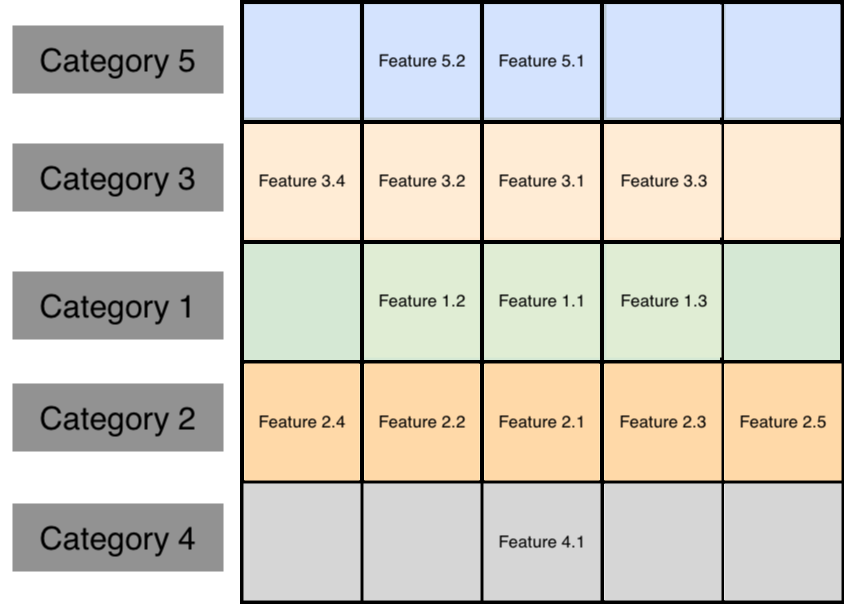
\includegraphics[width=10cm]{Figures/1stPaper/FV2I.png}
%	\caption{Example of positioning the elements in a matrix. Categories are assigned in rows based on their weight, and Features are assigned in the columns of the corresponding category based on their weight.}
%	\label{FV2IExample}
%\end{figure}

\underline{Entrenamientos}


Las figuras \ref{F1ScoreEvolution:1D} y \ref{F1ScoreEvolution:2D} muestran la evolución de la métrica de puntuación F1 a lo largo de las $100$ ejecuciones para las redes neuronales convolucionales 1D y 2D. Al visualizar la convolución unidimensional (Figura \ref{F1ScoreEvolution:1D}), se puedo verificar que la puntuación F1 de entrenamiento aumentaba ligeramente a lo largo de las épocas, experimentando altibajos a medida que el modelo se entrena, comenzando inicialmente con un valor de entrenamiento inferior a $0.58$ y llegando hasta $0.68$, mostrando poca capacidad de aprendizaje y generalización ante nuevas muestras.

 \begin{figure}[H]
	\centering
	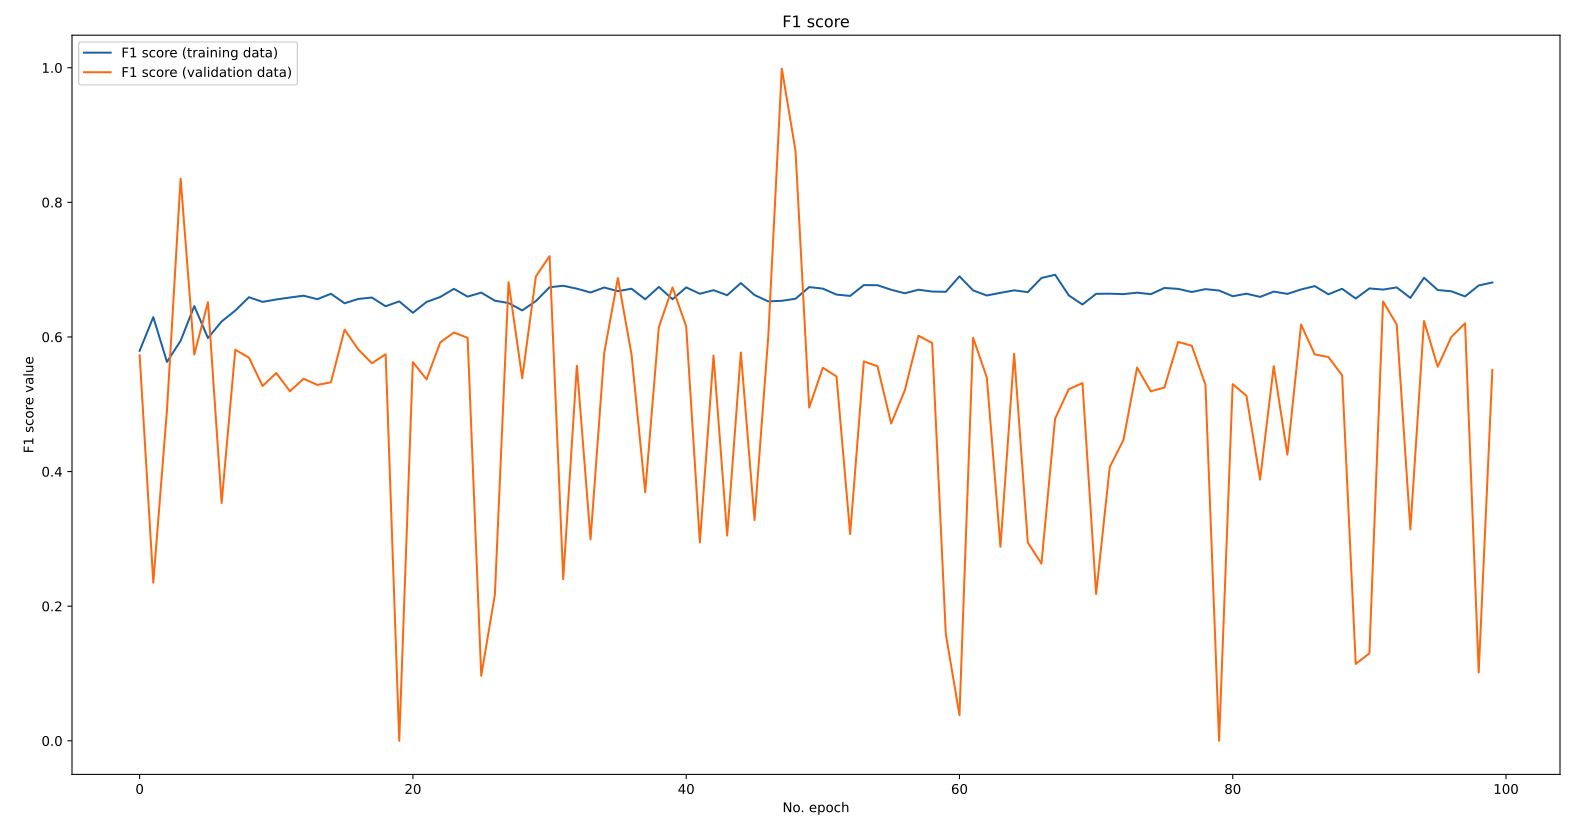
\includegraphics[width=14cm]{Figures/1stPaper/F1Score1D}
	\caption{Evolution of the F1-score of the 1D-CNN in the training and test set.}
	\label{F1ScoreEvolution:1D}
\end{figure}

Por otro lado, la Figura \ref{F1ScoreEvolution:2D} muestra el gráfico de entrenamiento y validación de la red neuronal convolucional bidimensional. Se observó que la tendencia de la función de pérdida en el conjunto de datos de entrenamiento era más estable. Se puede ver cómo la red, en la primera ejecución, comienza con un puntaje F1 de $0.62$ hasta alcanzar $0.78$ en la iteración $100$, por lo que se puede deducir que esta red logró un mejor rendimiento en el conjunto de entrenamiento en comparación con la red convolucional unidimensional, sufriendo menos altibajos respecto en el conjunto de validación.

\begin{figure}[H]
	\centering
	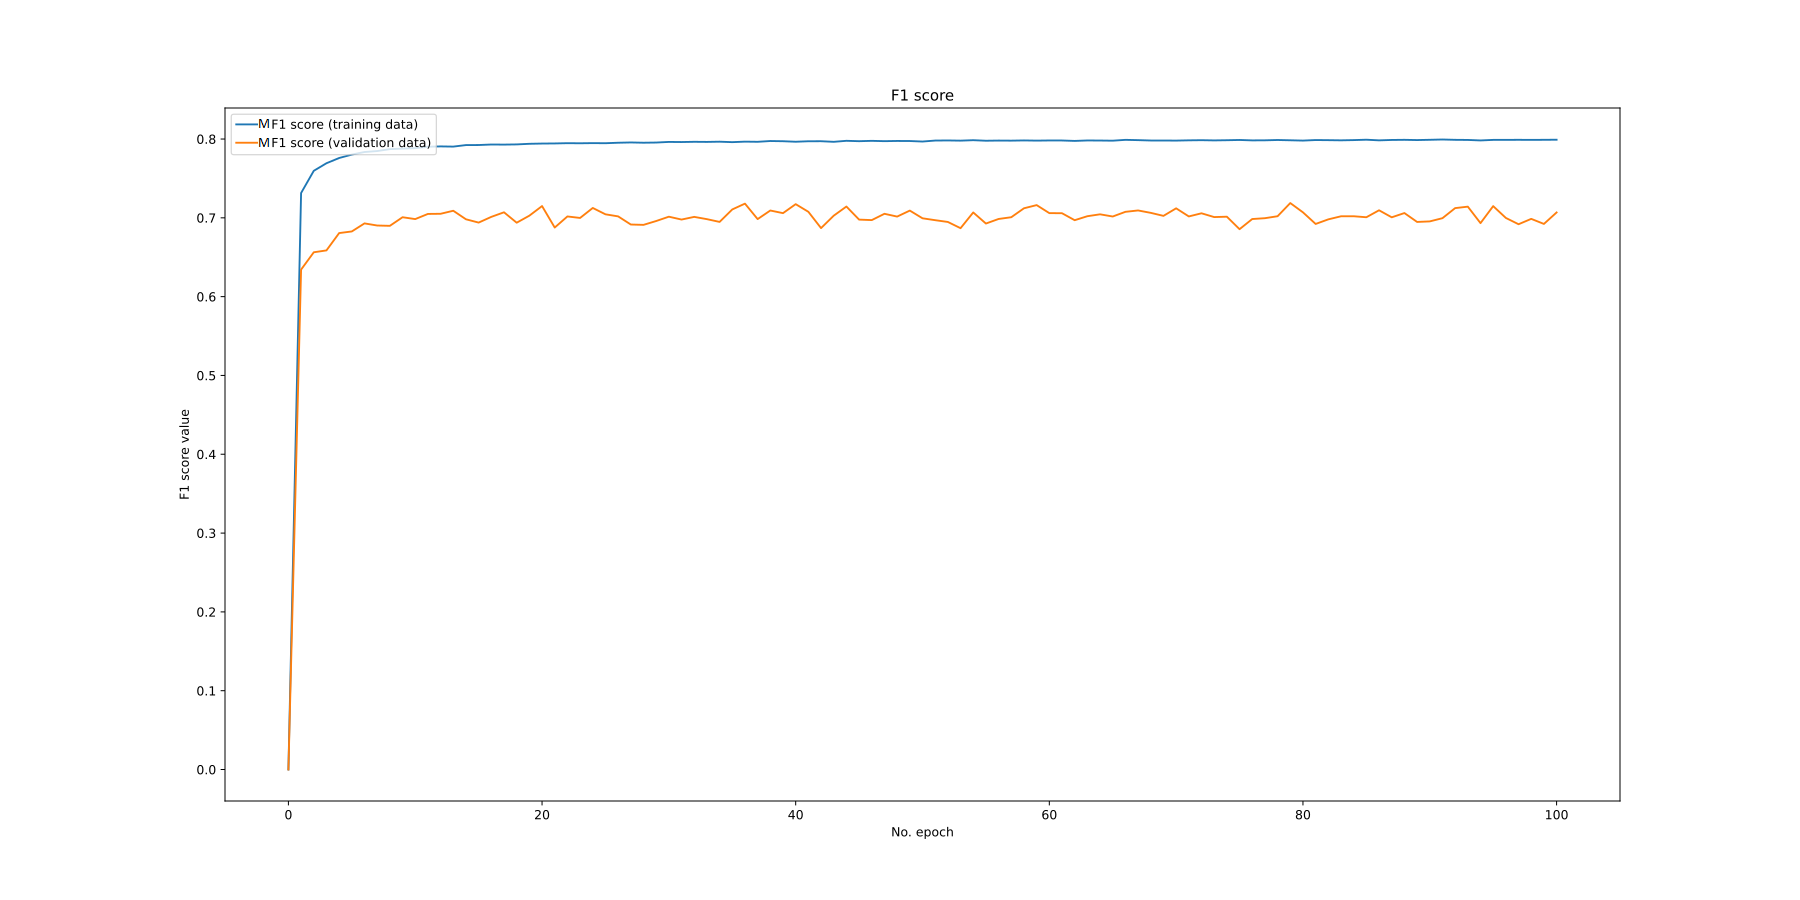
\includegraphics[width=14cm]{Figures/1stPaper/F1Score2D}
	\caption{Evolution of the F1-score of the 2D-CNN in training and test set.}
	\label{F1ScoreEvolution:2D}
\end{figure}


\underline{Resultados}
%%%%%%%%%%%%%%%%%%%%%%%%%%%%%%%%%%%%%%%%%%%%%%%%%%%%%%%%%%%%%%%%%%%%%%%%%%%%%%%%%%%%%%%%%%%%%%%%%%%%%%%%%%%%%%%%%%%%%%%%%%%%%%%%%%%%%%%%%%%%%%%%%%%%%%%%%%%%%%%%%%%%%%%%%%%%%%%%%%%%%%%%%%%%%%%%%%%%%%%%%%%%%%%%%%%%%%%%%%%%%%%%%%%%%%%%%%%%%%%%%%%%%%%%%%%%%%%%%%%%%%%%%%%%%%%%%%%%%%%%%%%%%%%%%%%%%%%%%%%%%%%%%%%%%%%%%%%%%%%%%%%%%%%%%%%%%%%%%%%
\begin{figure}[H]
	\centering
	\subfigure[Training 1D-CNN]{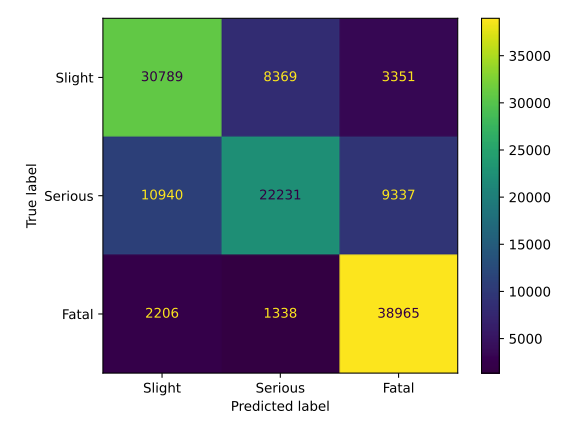
\includegraphics[width=60mm]{Figures/1stPaper/1DConfusionMatrixTrain.png}}
	\subfigure[Training 2D-CNN]{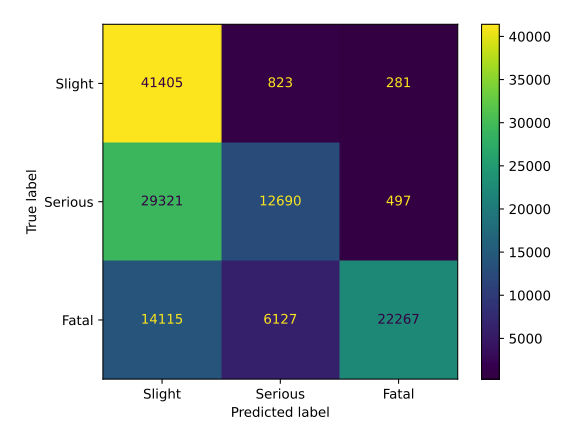
\includegraphics[width=60mm]{Figures/1stPaper/2DConfusionMatrixTrain.png}}
	\subfigure[Test 1D-CNN]{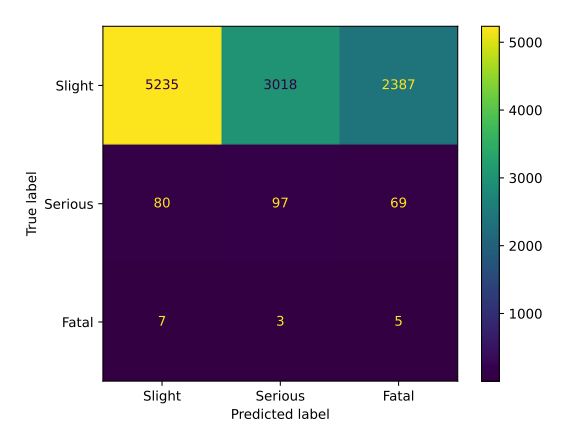
\includegraphics[width=60mm]{Figures/1stPaper/1DConfusionMatrixTest.png}}
	\subfigure[Test  2D-CNN]{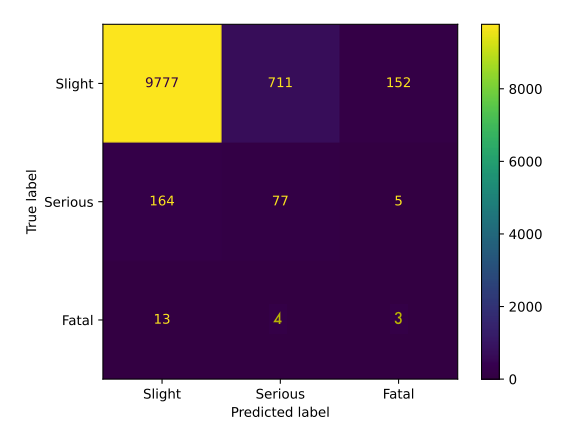
\includegraphics[width=60mm]{Figures/1stPaper/2DConfusionMatrixTest.png}}
	\caption{Confusion Matrices for Convolutional neural networks.}
	\label{ConfusionMatricesImages}
\end{figure}
%%%%%%%%%%%%%%%%%%%%%%%%%%%%%%%%%%%%%%%%%%%%%%%%%%%%%%%%%%%%%%%%%%%%%%%%%%%%%%%%%%%%%%%%%%%%%%%%%%%%%%%%%%%%%%%%%%%%%%%%%%%%%%%%%%%%%%%%%%%%%%%%%%%%%%%%%%%%%%%%%%%%%%%%%%%%%%%%%%%%%%%%%%%%%%%%%%%%%%%%%%%%%%%%%%%%%%%%%%%%%%%%%%%%%%%%%%%%%%%%%%%%%%%%%%%%%%%%%%%%%%%%%%%%%%%%%%%%%%%%%%%%%%%%%%%%%%%%%%%%%%%%%%%%%%%%%%%%%%%%%%%%%%%%%%%%%%%%%%%

\underline{Resultados}

Para evaluar el rendimiento de la metodología y los modelos propuestos, se realizó una comparación con tres modelos del estado del arte, el Gaussian Naive Bayes, Support Vector Classifier y K-Nearest Neighbor.

Los resultados de las métricas de clasificación se muestran en la Tabla \ref{ClassificationReportCNN:Test} para cada una de las clases predichas en el conjunto de \textbf{pruebas}. Estos informes muestran la información con la que evaluamos los modelos, ya que explica cómo se comportan con respecto a nuevos datos.

Como se puede ver en esta tabla, el modelo KNN obtiene mejores resultados en todas las medidas de todas las clases excepto en Recall en accidentes graves, donde el GNB es un poco mejor.

Si analizamos la métrica de Precisión, se puede observar que el modelo que presenta el mejor promedio para las clases Leves es la Red Neuronal Convolucional 1D (1D-CNN) con $0.984$, seguido por la Red Neuronal Convolucional 2D (2D-CNN) y el modelo KNN con $0.982$. Además, el 2D-CNN también ofrece la mejor métrica para accidentes graves con $0.097$, con una gran diferencia respecto al modelo KNN que le sigue con $0.042$. En cuanto a los accidentes fatales, tanto los modelos 1D-CNN como 2D-CNN tienen un valor similar, obteniendo $0.002$.

Respecto a la métrica de Recall, el mejor promedio para las clases Leves es la Red Neuronal Convolucional 2D (2D-CNN) con $0.919$, seguido por el modelo KNN con $0.689$. Además, el modelo GNB ofrece la mejor métrica para accidentes graves con $0.699$. En accidentes fatales, el 2D-CNN tiene el mejor valor con $0.1$.

Es necesario señalar que el F1-score es una forma de combinar las métricas de Precisión y Recall, y se define como la media armónica de la Precisión y Recall del modelo. Teniendo esto en cuenta, si analizamos el F1-score de los informes, el modelo que presenta el mejor promedio para las clases Leves es la Red Neuronal Convolucional 2D (2D-CNN), alcanzando $0.950$, muy por encima del siguiente modelo KNN, que ofrece un valor de $0.810$. Además, el 2D-CNN también ofrece la mejor métrica para accidentes graves con $0.148$, alcanzando el doble del rendimiento en comparación con el modelo que le sigue, el KNN con $0.076$. Respecto a los accidentes fatales, los modelos con la mejor clasificación son tanto la Red Neuronal Convolucional 1D como la 2D, obteniendo $0.004$, el doble que KNN, que son los siguientes mejores modelos en esta clase con $0.002$.

Podemos concluir que el modelo propuesto, basado en redes neuronales convolucionales, presenta mejores predicciones en cuanto a la métrica F1-score, que es una combinación de Precisión y Recall.

%%%%%%%%%%%%%%%%%%%%%%%%%%%%%%%%%%%%%%%%%%%%%%%%%%%%%%%%%%%%%%%%%%%%%%%%%%%%%%%%%
\begin{table}[H]
	\begin{center}
		\begin{tabular}{|c||c|c|c||c|c|c|}
			\hline
			\multicolumn{1}{ |c|| }{} & \multicolumn{3}{ |c|| }{\textbf{1D-CNN}} & \multicolumn{3}{ |c| }{\textbf{2D-CNN}} \\ \hline
			\textbf{Metric/Severity} & Slight & Serious & Fatal & Slight & Serious & Fatal
			\\ \hline \hline 
			Precision & \textcolor{blue}{0.701} & \textcolor{green}{0.696} & 0.754 & 0.488 & 0.646 & \textcolor{red}{0.966} \\ \hline 
			Recall & 0.724 & \textcolor{green}{0.523} & \textcolor{red}{0.917} & \textcolor{blue}{0.974} & 0.299 & 0.524\\ \hline 
			F1-score & \textcolor{blue}{0.712} & \textcolor{green}{0.597} & \textcolor{red}{0.828} & 0.650 & 0.409 & 0.679\\ \hline 
		\end{tabular}
	\end{center}
	\caption{Training metrics for 1D-CNN and 2D-CNN.}
	\label{ClassificationReportCNN:TrainCNN}
\end{table}

\begin{table}[H]
	\begin{center}
		\begin{tabular}{|c||c|c|c||c|c|c|}
			\hline
			\multicolumn{1}{ |c|| }{} & \multicolumn{3}{ |c|| }{\textbf{1D-CNN}} & \multicolumn{3}{ |c| }{\textbf{2D-CNN}} \\ \hline
			\textbf{Metric/Severity} & Slight & Serious & Fatal & Slight & Serious & Fatal
			\\ \hline \hline 
			Precision & \textcolor{blue}{0.984} & 0.031 & \textcolor{red}{0.002} & 0.982 & \textcolor{green}{0.097} & \textcolor{red}{0.002}\\ \hline 
			Recall & 0.429 & \textcolor{green}{0.394} & \textcolor{red}{0.333} & \textcolor{blue}{0.919} & 0.313 & 0.1\\ \hline 
			F1-score & 0.596 & 0.058 & \textcolor{red}{0.004} & \textcolor{blue}{0.950} & \textcolor{green}{0.148} & \textcolor{red}{0.004}\\ \hline 
		\end{tabular}
	\end{center}
	\caption{Test metrics for 1D-CNN and 2D-CNN.}
	\label{ClassificationReportCNN:TestCNN}
\end{table}
%%%%%%%%%%%%%%%%%%%%%%%%%%%%%%%%%%%%%%%%%%%%%%%%%%%%%%%%%%%%%%%%%%%%%%%%%%%%%%%%%

\underline{Resultados}



\begin{table}[H]
	\begin{center}
		\begin{tabular}{|c||c|c|c||c|c|c||c|c|c|}
			\hline
			\multicolumn{1}{ |c|| }{} & \multicolumn{3}{ |c|| }{\textbf{GNB}} & \multicolumn{3}{ |c|| }{\textbf{SVC}} & \multicolumn{3}{ |c| }{\textbf{KNN}} \\ \hline
			\textbf{Metric/Severity} & Slight & Serious & Fatal & Slight & Serious & Fatal & Slight & Serious & Fatal
			\\ \hline \hline 
			Precision & 0.980 & 0.025 & 0 & 0.979 & 0.029 & 0 & \textcolor{blue}{0.982} & \textcolor{green}{0.042} & \textcolor{red}{0.001} \\ \hline 
			Recall & 0.369 & \textcolor{green}{0.699} & 0 & 0.644 & 0.411 & 0 & \textcolor{blue}{0.689} & 0.382 & \textcolor{red}{0.067} \\ \hline 
			F1-score & 0.536 & 0.048 & 0 & 0.777 & 0.054 & 0 & \textcolor{blue}{0.810} & \textcolor{green}{0.076} & \textcolor{red}{0.002}\\ \hline 
		\end{tabular}
	\end{center}
	\caption{Test metrics classification for GNB, SVC and KNN.}
	\label{ClassificationReportCNN:Test}
\end{table}

\underline{Conclusiones}
\textcolor{red}{Trabajos a futuro en función de los resultados obtenidos, justificando el por qué de dichos cambios...}

Analizando los resultados de este artículo se propusieron una serie de mejoras a implementar para crear un modelo útil en la severidad de los accidentes, y aportar valor a los cuerpos de emergencia. Estos cambios a implementar fueron:

\begin{enumerate}
	\item Unión de la severidad original de los accidentes de tres clases a dos clases para paliar el efecto de la superposición en la clasificación. Concretamente realizar una agrupación de las clases Accidentes Severos y Accidentes Fatales a Necesidad de Asistencia.
	\item Inclusión de nuevas características para enriquecer la información con la que trabaja el modelo, tanto recopilación de nuevos datos como aplicar transformacioens sobre ellos para disponer de mayor información
	\item 
\end{enumerate}

\section{Resultados finales}

\underline{Aquí pones los resultados del paper 3}

En esta sección se expondrán los resultados ofrecidos por la metodología GTAAF, como se ha comentado anteriormente, esta metodología es una evolución del prototipo anterior. Para ello se analizarán los datos con los que se ha ejecutado este método, y los resultados de cada una de las etapas que lo componen aplicadas a estos datos.

\subsection{Dataset}

Los datos escogidos para esta tesis pertenecen a tres conjuntos de datos distintos, con el objetivo de poder evaluar la metodología y el nuevo modelo propuesto en diferentes contextos. Esta evaluación se basará en dos factores principales; la distinta disponibilidad de información en los datos, y en distintos casos de estudio en función de la densidad de población de las regiones escogidas. Teniendo en cuenta la densidad de población podemos distinguir entre tres casos de estudio claramente diferenciados: (1) alta concentración de población, (2) concentración media y (3) concentración dispersa. Con esta variabilidad en los datos se busca medir la robustez y generalización de la técnica desarrollada.

El primer dataset seleccionado contiene información de accidentes sobre la Comunidad de Madrid, donde se describen los accidentes de tráfico producidos entre 2019 y 2022 a lo largo de toda la comunidad. La alta densidad de población de Madrid convierte este conjunto de datos en un caso de estudio de alta concentración de población. Este conjunto de datos ha sido extraído del Portal de Datos Abiertos del Ayuntamiento de Madrid \cite{InfoDatasetMadrid}. 

El segundo caso de estudio contempla una situación de concentración de población dispersa, concretamente a lo largo del estado de Victoria, Australia, contemplando los accidentes producidos entre el 2000 y el 2005. Este conjunto de datos ha sido obtenido a través del Departamento de Transportes y Planificación del Gobierno de Victoria \cite{InfoDatasetVictoria}.

El tercer y último conjunto de datos pertenece al Departamento de Transportes de Reino Unido \cite{DatasetUK}, donde se contempla información de los accidentes producidos entre 2005 to 2020 a lo largo de todo el país. Sobre este conjunto de datos se han extraído accidentes pertenecientes a 6 regiones diferentes, concretamente: Southwark, Manchester, Birmingham, Liverpool, Sheffield y Cornwall. Cada una de ellas presenta un caso de uso distinto en función de su densidad de población. 


\subsection{Descripción de datos}

En esta sección se explicará la variabilidad en la disponibilidad de los datos entre los conjuntos de datos escogidos. Como se ha comentado anteriormente, cada uno de los datasets contiene distinta información en función de los recursos que disponga cada región, como puede ser la capacidad que se tenga para realizar pruebas de alcoholemia, la recogida de información de las condiciones actuales de la carretera o ...... entre otras, lo que provoca una heterogeneidad que debería ser tratada individualmente para cada población en específico . Para solventar este problema, y con el objetivo de crear una metodología y modelo predictivo generalizables a cualquier población independientemente de las características individuales que esta contenga, se propone agrupar las características disponibles en categorías fácilmente reconocibles. De esta forma, todos aquellos descriptores del accidente serán asignados a un concepto, donde cada uno de estos permite asignar características de muy fácil obtención, permitiendo así utilizar la metodología tanto para conjuntos de datos donde se disponga de información muy específica como para conjuntos de datos donde se contemple información más simplificada. Las categorías propuestas donde serán englobadas las características son las siguientes:

\begin{enumerate}
    \item Magnitud y ubicación del accidente: enfocado en información relativa a la localización y magnitud del accidente, como datos geográficos.
    \item Limitaciones de Conducción: abarcan características que limitan al conductor, como regulaciones realtivas a los límites de velocidad o condiciones actuales de la carretera.
    \item Factores ambientales: condiciones climáticas y de visibilidad.
    \item Información Temporal: relacionada con el momento del accidente.
    \item Información del Vehiculo: características que describan al vehículo objeto del accidente.
    \item Información de la Víctima: descriptores que definan a la víctima en el momento del incidente, factores como la edad, sexo, postiivo en sustancias estupefacientes, etc.
\end{enumerate}

En la Figura \ref{FeaturesClassification} se presentan las caracteristicas disponibles en cada uno de los conjuntos de datos escogidos en esta tesis, con el objetivo de mostrar la variabilidad de información que puede existir entre distintas poblaciones. Los campos marcados en naranja son aquellos que representan información distinta entre los datasets pero que pueden ser incluidos en las categorías correspondientes. Por otra parte, aquellos campos marcados en rojo indican la ausencia de este tipo de características en comparación con el resto de datasets.

\begin{figure}[H]
    \centering
    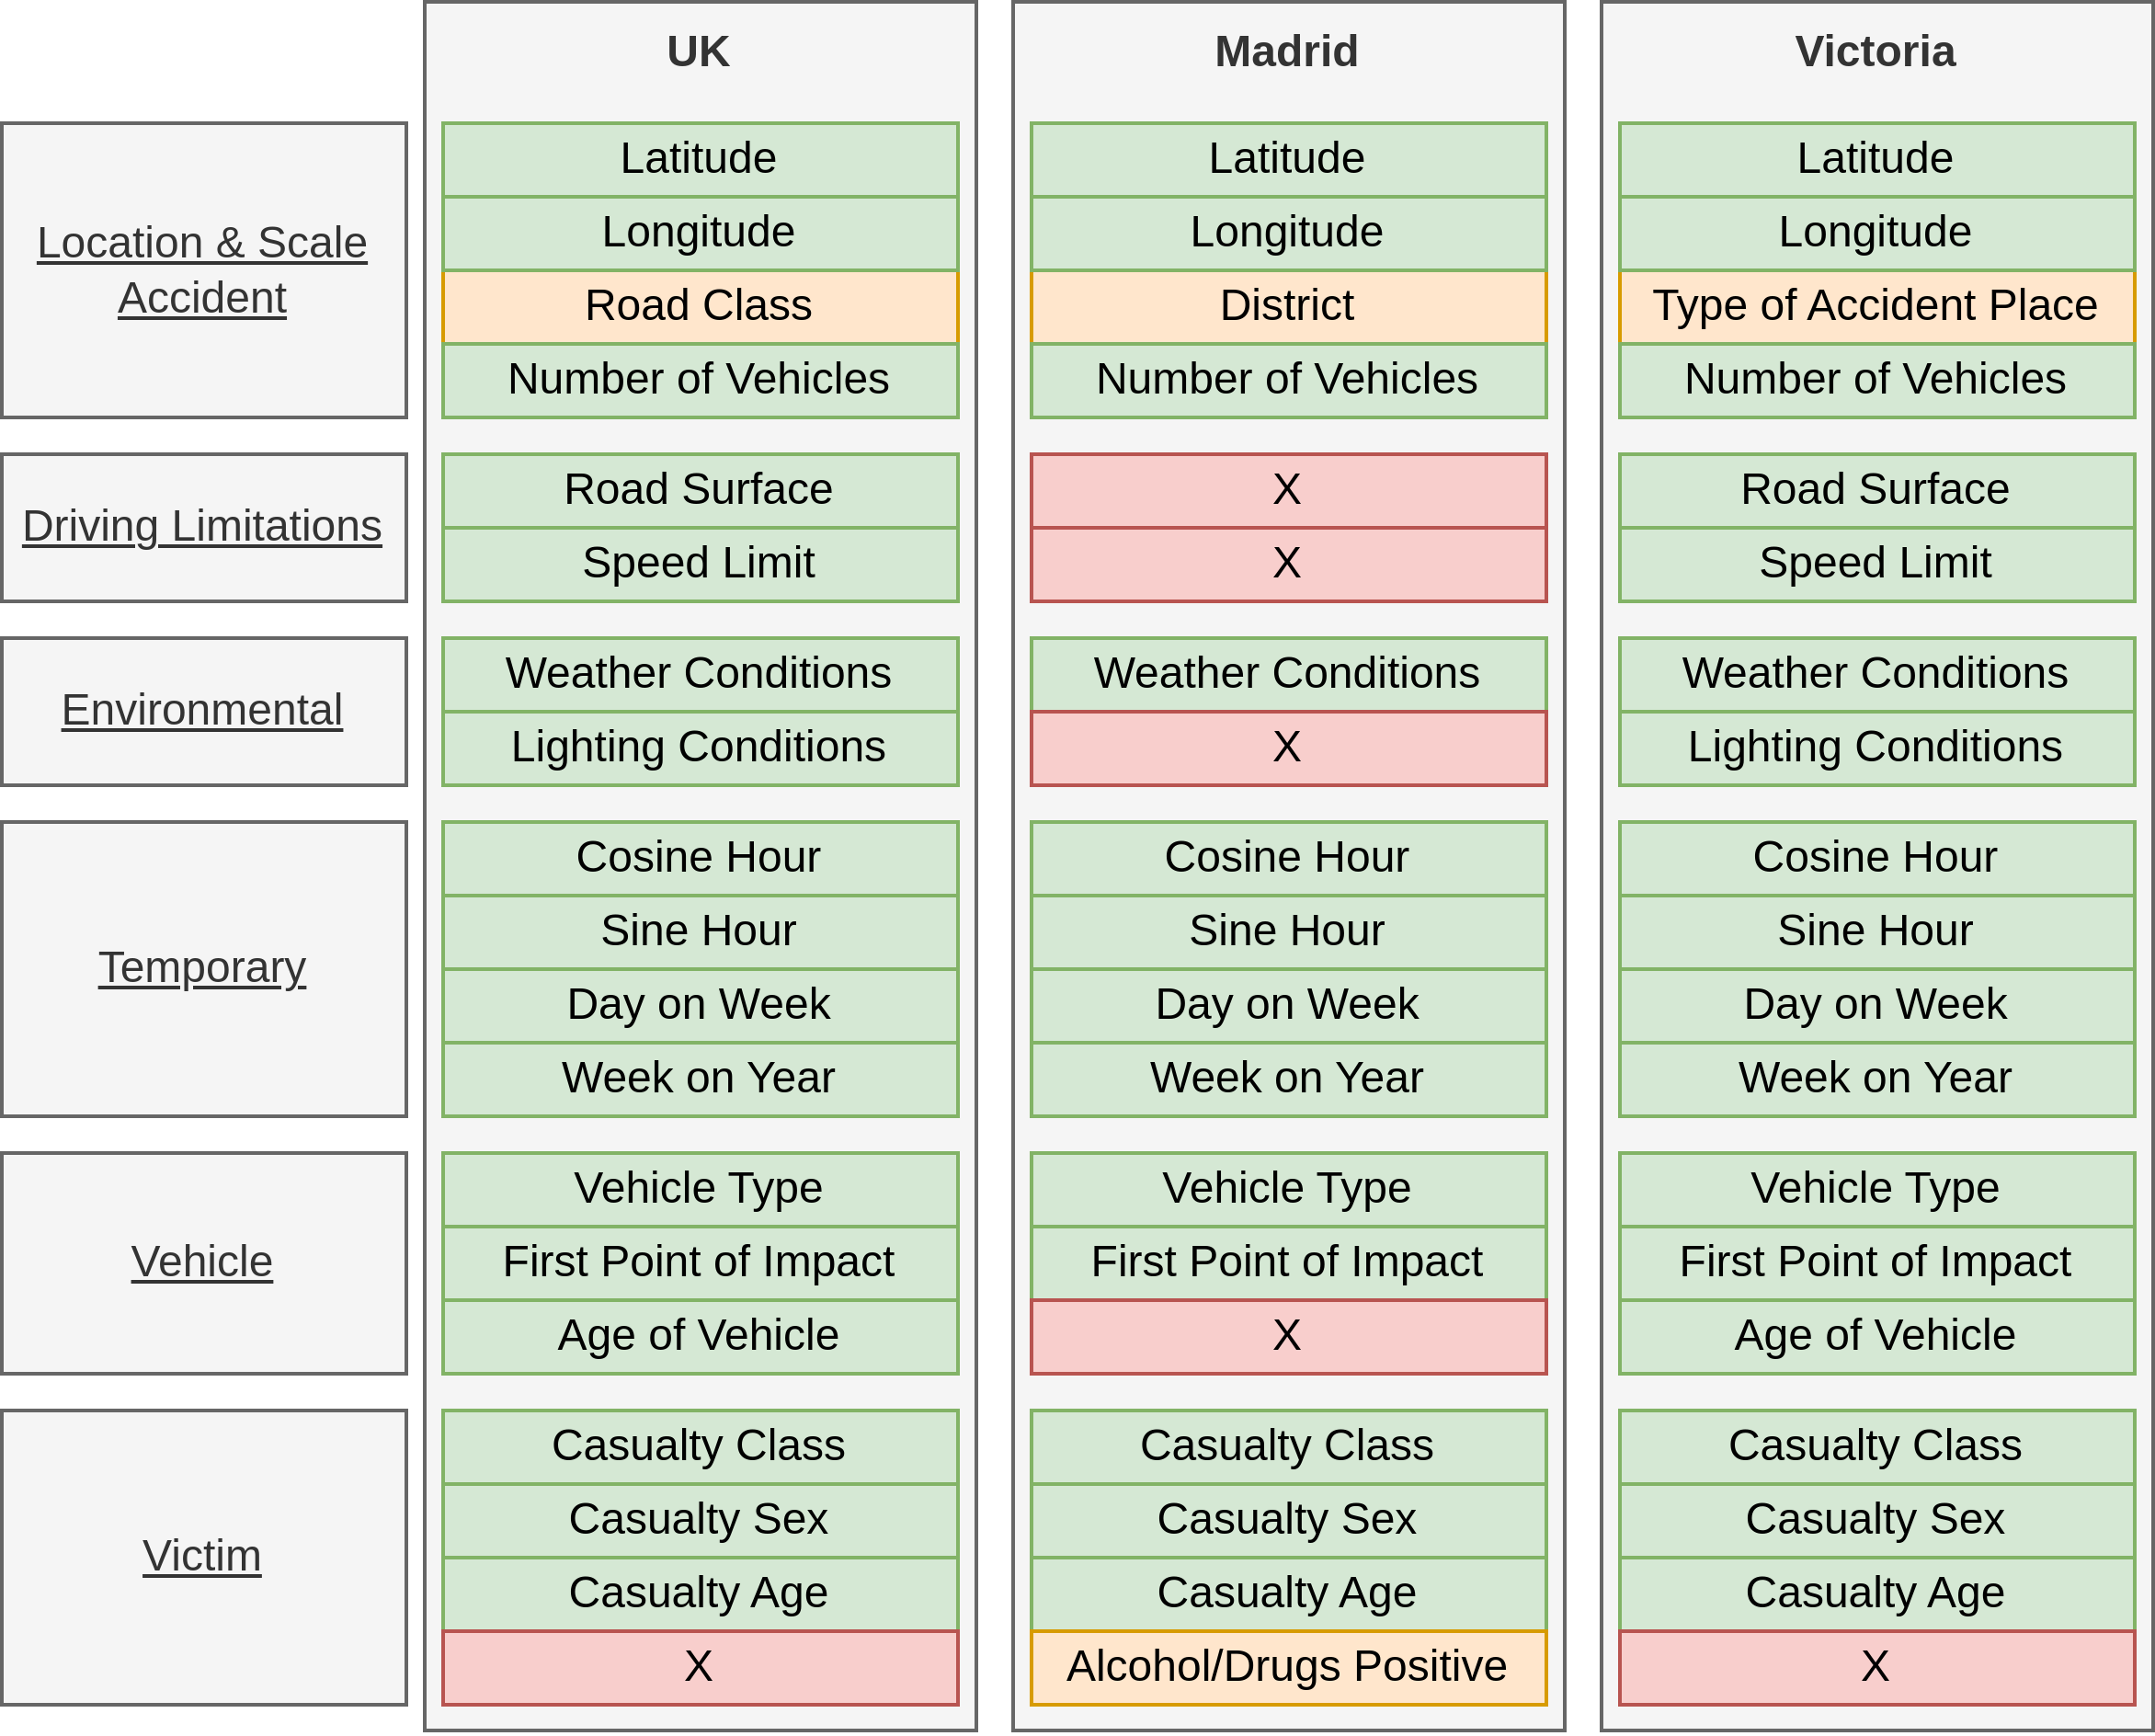
\includegraphics[width=14cm]{Figures/Dataset Comparative.png}
    \caption{Classification of variables. Fields shown in yellow represent features of the same nature but differing in data granularity. Additionally, missing features compared to other datasets are highlighted in red.}
    \label{FeaturesClassification}
\end{figure}

\subsubsection{Partes comunes entre los datos}

Normalmente, en cualquier conjunto de datos que describa accidentes, existe informacion básica y de fácil obtención que suele ser común entre distintas poblaciones.

Estas características comunes suelen ser información espacial, como es la localización del accidente, las condiciones climáticas en el momento del suceso y la hora y fecha en la que se ha producido. Por otra parte, como es lógico, exite informacion de fácil obtención que puede ser recogida rápidamente 'echando un vistazo rápido' al los vehículos implicados en el accidente, como es el tipo de vehículo colisionado y en cuál ha sido el primer punto de impacto.


\subsubsection{Principales diferencias entre los datos}

Como se puede observar, cada uno de los conjuntos de datos tiene una naturaleza diferente y ofrecen distinta información.

\textbf{UK}

En el caso de UK se observan ligeras diferencias respeto al resto de conjuntos de datos. Como es el caso de la característica Road class (para la categoría Location \& Scale Accident), cuyo significado varía en comparación con el resto de conjuntos de datos, y la ausencia de información sobre controles de estupefacientes a la víctima (categoría Victim). En el caso de Road Class, este campo representa la clasificacion de la carretera en la que se ha producido el accidente en base al tráfico que suelen contener. Esta clasificacion es responsabilidad de Gobierno de UK y se clasifican las vías en seis tipos diferentes: (1) Motorways: se trata de autopistas de alta velocidad que permiten el movimiento de vehículos entre los principales pueblos y ciudades. (2) A(M): se trata de carreteras principales que interconectan poblaciones y destinos de interés, estas vías pueden contener secciones transformadas en autovía. (3) A: carreteras importantes que conectan grandes densidades de tráfico entre zonas. Generalmente son las más anchas y directas, y son las de mayor importancia para el tráfico que contiene el área, estas carreteras pueden estar abiertas a distintos usuarios, como viandantes, ciclistas o caballos, aunque normalmente esto está restringido por las autoridades locales competentes. (4) Las carreteras B alimentan el tráfico entre las vías A y las carreteras más pequeñas de la red, siguen siendo de especial importancia para el tráfico, pero menos que las A. (5) Las carretereas tipo C son generalmente más pequeñas e interconectan las vías de tipo A y B. Normalmente unen urbanizaciones con el resto de carreteras de la red, son carreteras de menor importancia que las anteriores pero son de mayor relevancia respecto a las del siguiente tipo. (6) Carreteras no clasificadas, se tratan de vías destinadas al tráfico local, por su naturaleza la mayoría de las vías pertenecen a este tipo, generalmente tienen muy poca importancia y a nivel local \cite{UKDepartmentForTransportRoadClassification}.


\textbf{Madrid}

En el caso del conjunto de datos de Madrid, las diferencias respecto al resto de datasets es más notable. La información disponible es considerablemente menor en comparación con el dataset de UK y de Victoria. Analizando la Figura se puede observar que hay ciertas características que no están presentes, llegando a dejar incluso una categoría vacía (Driving Limitations) al no disponer de infromación de este tipo. Por otra parte, tampoco se dispone de la información de Lighting Conditions para la categoría Environmental ni de Age of Vehicle, en la categoría de caracterísitcas del vehiculo. No obstante, aún faltando esta información, el resto de características pueden ser asignadas a las categorías definidas, convirtiendo, por tanto, este dataset aplicable a esta metodología.

Sin embargo, el conjunto de datos de Madrid ofrece información sobre si la víctima se encuentra bajo los efectos del alcohol o de sustancias estupefacientes. Al ser un dato que describe a la víctima del incidente, este será asignado a la categoría Victim.

Por otro lado, en la cateogría Location \& Scale Accident los datos de Madrid presentan una diferencia en lo que representa la característica District respecto al resto de datasets. Este campo ha sido obtenido mediante expresiones regulares, buscando distintos tipos de vía sobre la columna que ofrece información acerca del nombre de la calle. De tal forma que contiene engloba información del tipo de vía urbana o interurbana sobre la que transitaba el vehículo en el momento en el que se produjo el accidente, como avenidas, boulevares, entre otras. Al ser una característica que ofrece información sobre la localización del accidente, será incluída en la categoría de Location \& Scale Accident. En la tabla X de anexos pueden consultarse los distintos valores que esta característica puede tomar.

\textbf{Victoria}

El conjunto de datos de Victoria contempla un caso parecido al de los datos de UK, donde no se disponen de datos que describan si la víctima se encontraba bajo los efectos de estupefacientes o del alcohol, como es el caso del conjunto de datos de Madrid. Por lo que esta característica quedará vacía también en el dataset de Victoria.

Por otra parte, la característica Type Of Accident Place, ofrece información sobre el lugar del accidente, concretamente el lugar donde se ha producido, como autopista, parking, tunel, etc. por lo que irá asignada a la categoría Location \& Scale Accident.


\subsection{Limpieza}
 En la tabla \ref{DataDistribution} se expone el número total de registros del conjunto de datos original y el número de muestras resultante tras haber aplicado la limpieza de estos datos para cada una de las poblaciones contempladas en esta tesis.


\begin{table}[H]
	\begin{center}
		\begin{tabular}{|c|c||c|c|}
		\hline
		\multicolumn{4}{ |c| }{\textbf{Data Distribution}} \\ \hline
		\multicolumn{4}{ |c| }{\textbf{UK}} \\ \hline

		\textbf{Region} & \textbf{Assistance} & Original & Cleaned
        \\ \hline \hline

        \multirow{2}{*}{Southwark} &
            No  & X  & X  \\ &
            Yes & X  & X \\ \hline \hline
        \multirow{2}{*}{Manchester} &
            No  & X & X \\ &
            Yes & X & X \\ \hline \hline
        \multirow{2}{*}{Birmingham} &
            No  & X  & X \\ &
            Yes & X  & X \\ \hline \hline
        \multirow{2}{*}{Liverpool} &
            No  & X  & X \\ &
            Yes & X  & X \\ \hline \hline
        \multirow{2}{*}{Sheffield} &
            No  & X  & X  \\ &
            Yes & X  & X \\ \hline \hline
        \multirow{2}{*}{Cornwall} &
            No  & X & X  \\ &
            Yes & X & X \\ \hline \hline

		\multicolumn{4}{ |c| }{\textbf{Spain}} \\ \hline

		\textbf{Region} & \textbf{Assistance} & Original & Filtered
		\\ \hline \hline

        \multirow{2}{*}{Madrid} &
            No  & X  & X   \\ &
            Yes & X  & X  \\ \hline \hline

		\multicolumn{4}{ |c| }{\textbf{Australia}} \\ \hline

		\textbf{Region} & \textbf{Assistance} & Original & Filtered
		\\ \hline \hline

        \multirow{2}{*}{Victoria} &
            No   & X  & X   \\ &
            Yes  & X & X \\ \hline \hline
            
		\end{tabular}
	\caption{XX}
	\label{DataDistribution}
	\end{center}
 \end{table}

Como se puede observar, la población que más valores nulos presenta en las categorías de interés es la ciudad de XX, obteniendo una pérdida del X\% respecto al conjunto de datos incial...

En la Figura X se muestra una representación visual del número de registros previo al proceso de limpieza respecto al resultado de esta etapa.
(Histogramas pre y post limpieza?).


\subsection{Filtrado de áreas}


Para ilustrar los parámetros con los que se aplica el filtrado de áreas, se presenta la Tabla \ref{AreasInformation}, donde se muestra para cada población el número de áreas por las que pasará el filtro, además del tamaño de la ventana X,Y para cada región, donde en función de la extensión y la densidad de población tomará valores más grandes (poblaciones más dispersas) o valores más pequeños (cuando la densidad de población es alta). Los tamaños de ventana para cada población han sido escogidos mediante un procedimiento experimetal, en el que se maximiza el rendimiento final de los modelos.

\begin{table}[H]
	\begin{center}
		\begin{tabular}{|c|c||c|c|c||c|c|c}
		\hline
		\multicolumn{4}{ |c| }{\textbf{Areas Split}} \\ \hline

		\multicolumn{4}{ |c| }{\textbf{UK}} \\ \hline
		\textbf{City} & \textbf{Axis} & \textbf{Areas Number} & \textbf{Areas Size}
		\\ \hline  \hline 

        \multirow{2}{*}{Southwark} &
            X  & 529  & 10 \\ &
            Y  & 487  & 20 \\ \hline \hline
        \multirow{2}{*}{Manchester} &
            X  & 791     & 14  \\ &
            Y  & 1069    & 20  \\ \hline \hline
        \multirow{2}{*}{Birmingham} &
            X  & 3519    & 12 \\ &
            Y  & 1557    & 17 \\ \hline \hline
        \multirow{2}{*}{Liverpool} &
            X  & 2107    & 12  \\ &
            Y  & 717     & 21  \\ \hline \hline
        \multirow{2}{*}{Sheffield} &
            X  & 1896     & 12  \\ &
            Y  & 1115     & 18 \\ \hline \hline
        \multirow{2}{*}{Cornwall} &
            X  & 10090    & 15 \\ &
            Y  & 5597    & 19 \\ \hline \hline

		\multicolumn{4}{ |c| }{\textbf{Spain}} \\ \hline
		\textbf{City} & \textbf{Axis} & \textbf{Areas Number} & \textbf{Areas Size}
		\\ \hline  \hline 

        \multirow{2}{*}{Madrid} &
            X  & 5241  & 5 \\ &
            Y  & 4444  & 7 \\ \hline \hline

		\multicolumn{4}{ |c| }{\textbf{Australia}} \\ \hline
		\textbf{City} & \textbf{Axis} & \textbf{Areas Number} & \textbf{Areas Size}
		\\ \hline  \hline 

        \multirow{2}{*}{Victoria} &
            X  & 4931  & 145 \\ &
            Y  & 5241  & 97 \\ \hline \hline
		\end{tabular}
	\end{center}
	\caption{}
	\label{AreasInformation}
\end{table}

Una vez se establecen las dimensiones de las ventanas de tamaño X,Y se aplica el filtrado para cada ciudad, donde el número de muestras de la clase mayoritaria se ve considerablmente rebajado respecto a la minoritaria, con el objetivo de tener un conjunto de datos más balanceado. La tabla \ref{DataDistribution} muestra el número de registros original para cada población y el número de registros resultante tras aplicar el filtrado por áreas.

%%%%%%%%%%%%%%%%%%%%%%%%%%%%%%%%%%%%%%%%%%%%%%%%%%%%%%%%%%%%%%%%%%%%%%%%%%%%%%%%%
\begin{table}[H]
	\begin{center}
		\begin{tabular}{|c|c||c|c|}
		\hline
		\multicolumn{4}{ |c| }{\textbf{Data Distribution}} \\ \hline
		\multicolumn{4}{ |c| }{\textbf{UK}} \\ \hline

		\textbf{Region} & \textbf{Assistance} & Original & Filtered
		\\ \hline \hline

        \multirow{2}{*}{Southwark} &
            No   & 27105  & 4251 \\ &
            Yes  & 3109   & 1256 \\ \hline \hline
        \multirow{2}{*}{Manchester} &
            No  & 48771   & 4548 \\ &
            Yes & 4570 & 1466 \\ \hline \hline
        \multirow{2}{*}{Birmingham} &
            No  & 108723  & 4092 \\ &
            Yes & 11187   & 2063 \\ \hline \hline
        \multirow{2}{*}{Liverpool} &
            No  & 49291  & 3640 \\ &
            Yes & 5161   & 1192 \\ \hline \hline
        \multirow{2}{*}{Sheffield} &
            No  & 43579  & 2060  \\ &
            Yes & 5887  & 1638  \\ \hline \hline
        \multirow{2}{*}{Cornwall} &
            No  & 32994 & 2191 \\ &
            Yes & 4852 & 2020 \\ \hline \hline

		\multicolumn{4}{ |c| }{\textbf{Spain}} \\ \hline

		\textbf{Region} & \textbf{Assistance} & Original & Filtered
		\\ \hline \hline

        \multirow{2}{*}{Madrid} &
            No   & 53218  & 2601 \\ &
            Yes  & 1355   & 1286 \\ \hline \hline

		\multicolumn{4}{ |c| }{\textbf{Australia}} \\ \hline

		\textbf{Region} & \textbf{Assistance} & Original & Filtered
		\\ \hline \hline

        \multirow{2}{*}{Victoria} &
            No   & 4857  & 2065  \\ &
            Yes  & 5609  & 2649  \\ \hline \hline
            
		\end{tabular}
	\end{center}
	\caption{}
	\label{DataDistribution}
\end{table}

\textbf{Luis:} Para mí aquí irían ya los mapas del tercer paper..
(Mapas)


En la figura X se puede observar la distribución de clases para cada población
(Poner aquí un histograma del desbalanceo de las clases y justo al lado la distribución una vez se aplica el filtrado de áreas.)


\subsection{Discretización}


Tabla de discretización.

\underline{UK}
UK discretización
%%%%%%%%%%%%%%%%%%%%%%%%%%%%%%%%%%%%%%%%%%%%%%%%%%%%%%%%%%%%%%%%%%%%%%%%%%%%%%%%%
 \begin{table}[H]
    \small
    \begin{center}
    \begin{tabular}{|c|c|c|c|}
        \hline
        \textbf{Classification} & \textbf{Feature} & \textbf{Typing} & \textbf{Value} \\ \hline 
        \hline

        \multirow{9}{*}{\textbf{\makecell{Location \& \\ Scale Accident}}}
            & Latitude  & Real Number & OSGR East Coordinate \\ \cline{2-4}
            & Longitude & Real Number & OSGR North Coordinate \\ \cline{2-4}
            & \multirow{6}{*} {Road Class}
                               & 0 & Motorway \\ \cline{3-4}
                              && 1 & A(M) \\ \cline{3-4}
                              && 2 & A \\ \cline{3-4}
                              && 3 & B \\ \cline{3-4}
                              && 4 & C \\ \cline{3-4}
                              && 5 & Unclassified \\ \cline{2-4}
            & Number of Vehicles & 0-N & Depending on the number of vehicles involved \\ \cline{2-4}

        \hline
        \hline


        \multirow{6}{*}{\textbf{\makecell{Driving \\ Limitations}}}
            & \multirow{5}{*} {Road Surface}
                          & 0 & Dry \\ \cline{3-4}
                         && 1 & Wet / Damp \\ \cline{3-4}
                         && 2 & Snow \\ \cline{3-4}
                         && 3 & Frost / Ice \\ \cline{3-4}
                         && 4 & Flood  \\ \cline{2-4}
            & Speed Limit & 0-70 & Depending on the speed limit (mph) of the road \\ \cline{2-4}

        \hline
        \hline

        \multirow{13}{*}{\textbf{\makecell{Environmental}}} 
            & \multirow{8}{*} {Weather Conditions}
                          & 0 & Fine without high winds \\ \cline{3-4}
                         && 1 & Raining without high winds \\ \cline{3-4}
                         && 2 & Snowing without high winds \\ \cline{3-4}
                         && 3 & Fine with high winds \\ \cline{3-4}
                         && 4 & Raining with high winds \\ \cline{3-4}
                         && 5 & Snowing with high winds \\ \cline{3-4}
                         && 6 & Fog or mist \\ \cline{3-4}
                         && 7 & Other  \\ \cline{2-4}

            & \multirow{5}{*} {Lighting Conditions}
                                  & 0 & Daylight: street lights present \\ \cline{3-4}
                                 && 1 & Darkness: no street lighting \\ \cline{3-4}
                                 && 2 & Darkness: street lights present and lit \\ \cline{3-4}
                                 && 3 & Darkness: street lights present but unlit \\ \cline{3-4}
                                 && 4 & Darkness: street lighting unknown  \\ \cline{2-4}

        \hline
        \hline

        \multirow{4}{*}{\textbf{\makecell{Temporary}}} 
            & Cosine Hour & Real Number & XX \\ \cline{2-4}
            & Sine Hour & Real Number & XX \\ \cline{2-4}
            & Day on Week & 0-6 & XX \\ \cline{2-4}
            & Week on Year & 0-52 & XX \\ \cline{2-4}

        \hline
        \hline

        \multirow{7}{*}{\textbf{Vehicle}}
            & Vehicle Type & 0-17 & Depending on the weight of the vehicle \\ \cline{2-4}
            & \multirow{5}{*} {First Point of Impact}
                                  & 0 & Did not impact \\ \cline{3-4}
                                 && 1 & Front \\ \cline{3-4}
                                 && 2 & Back \\ \cline{3-4}
                                 && 3 & Offside \\ \cline{3-4}
                                 && 4 & Nearside \\ \cline{3-4}
                                 && 5 & Unknown (self reported) \\ \cline{2-4}
            & Age of Vehicle  & 0-N & In order of vehicle age \\ \cline{2-4}

        \hline
        \hline

        \multirow{9}{*}{\textbf{Victim}}
            & \multirow{3}{*} {Casualty Class}
                             & 0 & Driver/Rider \\ \cline{3-4}
                            && 1 & Passenger \\ \cline{3-4}
                            && 2 & Pedestrian  \\ \cline{2-4}
            & \multirow{2}{*} {Casualty Sex}
                          & 0 & Male \\ \cline{3-4}
                         && 1 & Female  \\ \cline{2-4}
            & \multirow{4}{*} {Casualty Age}
                             & 0 & Younger than 18 \\ \cline{3-4}
                            && 1 & Between 18 and 25 \\ \cline{3-4}
                            && 2 & Between 25 and 65 \\ \cline{3-4}
                            && 3 & Older than 65  \\ \cline{2-4}

        \hline
        \hline
    \end{tabular}
    \end{center}
    \caption{UK classification of variables.}
    \label{UKFeaturesClassification}
\end{table}
%%%%%%%%%%%%%%%%%%%%%%%%%%%%%%%%%%%%%%%%%%%%%%%%%%%%%%%%%%%%%%%%%%%%%%%%%%%%%%%%%

\underline{Madrid}
Madrid discretización, in progress...
%%%%%%%%%%%%%%%%%%%%%%%%%%%%%%%%%%%%%%%%%%%%%%%%%%%%%%%%%%%%%%%%%%%%%%%%%%%%%%%%%
 \begin{table}[H]
    \small
    \begin{center}
    \begin{tabular}{|c|c|c|c|}
        \hline
        \textbf{Classification} & \textbf{Feature} & \textbf{Typing} & \textbf{Value} \\ \hline 
        \hline

        \multirow{4}{*}{\textbf{\makecell{Location \& \\ Scale Accident}}}
            & Latitude  & Real Number & Cartesian coordinate system \\ \cline{2-4}
            & Longitude & Real Number & Cartesian coordinate system \\ \cline{2-4}
            & District  & 0-X & District number (Anexo 1*) \\ \cline{2-4}
            & Number of Vehicles & 0-N & Depending on the number of vehicles involved \\ \cline{2-4}
        \hline
        \hline

        \multirow{13}{*}{\textbf{\makecell{Environmental}}} 
            & \multirow{8}{*} {Weather Conditions}
                          & 0 & Fine without high winds \\ \cline{3-4}
                         && 1 & Raining without high winds \\ \cline{3-4}
                         && 2 & Snowing without high winds \\ \cline{3-4}
                         && 3 & Fine with high winds \\ \cline{3-4}
                         && 4 & Raining with high winds \\ \cline{3-4}
                         && 5 & Snowing with high winds \\ \cline{3-4}
                         && 6 & Fog or mist \\ \cline{3-4}
                         && 7 & Other  \\ \cline{2-4}


        \hline
        \hline

        \multirow{4}{*}{\textbf{\makecell{Temporary}}} 
            & Cosine Hour & Real Number & XX \\ \cline{2-4}
            & Sine Hour & Real Number & XX \\ \cline{2-4}
            & Day on Week & 0-6 & XX \\ \cline{2-4}
            & Week on Year & 0-52 & XX \\ \cline{2-4}

        \hline
        \hline

        \multirow{6}{*}{\textbf{Vehicle}}
            & Vehicle Type & 0-17 & Depending on the weight of the vehicle \\ \cline{2-4}
            & \multirow{5}{*} {First Point of Impact}
                                & 1 &  Head-on - size collision  \\ \cline{3-4}
                                && 2 &  Rear-end collision \\ \cline{3-4}
                                && 3 &  Side crash \\ \cline{3-4}
                                && 4 &  Collision again fixed obstacle \\ \cline{3-4}
                                && 5 &  Pile-up \\ \cline{3-4}
                                && 6 &  Hitting a pedestrian \\ \cline{3-4}
                                && 7 &  Head-on collision \\ \cline{3-4}
                                && 8 &  Other \\ \cline{3-4}
                                && 9 &  Leaving the road \\ \cline{3-4}
                                && 10 &  Vehicle rollover \\ \cline{3-4}
                                && 11 &  Hitting an animal \\ \cline{3-4}
                                && 12 &  Falling \\ \cline{3-4}
        \hline
        \hline

        \multirow{9}{*}{\textbf{Victim}}
            & \multirow{3}{*} {Casualty Class}
                             & 0 & Driver/Rider \\ \cline{3-4}
                            && 1 & Passenger \\ \cline{3-4}
                            && 2 & Pedestrian  \\ \cline{2-4}
            & \multirow{2}{*} {Casualty Sex}
                          & 0 & Male \\ \cline{3-4}
                         && 1 & Female  \\ \cline{2-4}
            & \multirow{4}{*} {Casualty Age}
                             & 0 & Younger than 18 \\ \cline{3-4}
                            && 1 & Between 18 and 25 \\ \cline{3-4}
                            && 2 & Between 25 and 65 \\ \cline{3-4}
                            && 3 & Older than 65  \\ \cline{2-4}
            & \multirow{2}{*} {Alcohol/Drugs Positive}
                             & 0 & No \\ \cline{3-4}
                            && 1 & Yes \\ \cline{3-4}
        \hline
        \hline
    \end{tabular}
    \end{center}
    \caption{Victoria classification of variables.}
    \label{VictoriaFeaturesClassification}
\end{table}
%%%%%%%%%%%%%%%%%%%%%%%%%%%%%%%%%%%%%%%%%%%%%%%%%%%%%%%%%%%%%%%%%%%%%%%%%%%%%%%%%

\underline{Victoria}

Victoria discretización, in progres...

%%%%%%%%%%%%%%%%%%%%%%%%%%%%%%%%%%%%%%%%%%%%%%%%%%%%%%%%%%%%%%%%%%%%%%%%%%%%%%%%%
 \begin{table}[H]
    \small
    \begin{center}
    \begin{tabular}{|c|c|c|c|}
        \hline
        \textbf{Classification} & \textbf{Feature} & \textbf{Typing} & \textbf{Value} \\ \hline 
        \hline

        \multirow{9}{*}{\textbf{\makecell{Location \& \\ Scale Accident}}}
            & Latitude  & Real Number & OSGR East Coordinate \\ \cline{2-4}
            & Longitude & Real Number & OSGR North Coordinate \\ \cline{2-4}
            & \multirow{6}{*} {Road Class}
                               & 0 & Motorway \\ \cline{3-4}
                              && 1 & A(M) \\ \cline{3-4}
                              && 2 & A \\ \cline{3-4}
                              && 3 & B \\ \cline{3-4}
                              && 4 & C \\ \cline{3-4}
                              && 5 & Unclassified \\ \cline{2-4}
            & Number of Vehicles & 0-N & Depending on the number of vehicles involved \\ \cline{2-4}

        \hline
        \hline


        \multirow{6}{*}{\textbf{\makecell{Driving \\ Limitations}}}
            & \multirow{5}{*} {Road Surface}
                          & 0 & Dry \\ \cline{3-4}
                         && 1 & Wet / Damp \\ \cline{3-4}
                         && 2 & Snow \\ \cline{3-4}
                         && 3 & Frost / Ice \\ \cline{3-4}
                         && 4 & Flood  \\ \cline{2-4}
            & Speed Limit & 0-70 & Depending on the speed limit (mph) of the road \\ \cline{2-4}

        \hline
        \hline

        \multirow{13}{*}{\textbf{\makecell{Environmental}}} 
            & \multirow{8}{*} {Weather Conditions}
                          & 0 & Fine without high winds \\ \cline{3-4}
                         && 1 & Raining without high winds \\ \cline{3-4}
                         && 2 & Snowing without high winds \\ \cline{3-4}
                         && 3 & Fine with high winds \\ \cline{3-4}
                         && 4 & Raining with high winds \\ \cline{3-4}
                         && 5 & Snowing with high winds \\ \cline{3-4}
                         && 6 & Fog or mist \\ \cline{3-4}
                         && 7 & Other  \\ \cline{2-4}

            & \multirow{5}{*} {Lighting Conditions}
                                  & 0 & Daylight: street lights present \\ \cline{3-4}
                                 && 1 & Darkness: no street lighting \\ \cline{3-4}
                                 && 2 & Darkness: street lights present and lit \\ \cline{3-4}
                                 && 3 & Darkness: street lights present but unlit \\ \cline{3-4}
                                 && 4 & Darkness: street lighting unknown  \\ \cline{2-4}

        \hline
        \hline

        \multirow{4}{*}{\textbf{\makecell{Temporary}}} 
            & Cosine Hour & Real Number & XX \\ \cline{2-4}
            & Sine Hour & Real Number & XX \\ \cline{2-4}
            & Day on Week & 0-6 & XX \\ \cline{2-4}
            & Week on Year & 0-52 & XX \\ \cline{2-4}

        \hline
        \hline

        \multirow{7}{*}{\textbf{Vehicle}}
            & Vehicle Type & 0-17 & Depending on the weight of the vehicle \\ \cline{2-4}
            & \multirow{5}{*} {First Point of Impact}
                                  & 0 & Did not impact \\ \cline{3-4}
                                 && 1 & Front \\ \cline{3-4}
                                 && 2 & Back \\ \cline{3-4}
                                 && 3 & Offside \\ \cline{3-4}
                                 && 4 & Nearside \\ \cline{3-4}
                                 && 5 & Unknown (self reported) \\ \cline{2-4}
            & Age of Vehicle  & 0-N & In order of vehicle age \\ \cline{2-4}

        \hline
        \hline

        \multirow{9}{*}{\textbf{Victim}}
            & \multirow{3}{*} {Casualty Class}
                             & 0 & Driver/Rider \\ \cline{3-4}
                            && 1 & Passenger \\ \cline{3-4}
                            && 2 & Pedestrian  \\ \cline{2-4}
            & \multirow{2}{*} {Casualty Sex}
                          & 0 & Male \\ \cline{3-4}
                         && 1 & Female  \\ \cline{2-4}
            & \multirow{4}{*} {Casualty Age}
                             & 0 & Younger than 18 \\ \cline{3-4}
                            && 1 & Between 18 and 25 \\ \cline{3-4}
                            && 2 & Between 25 and 65 \\ \cline{3-4}
                            && 3 & Older than 65  \\ \cline{2-4}

        \hline
        \hline
    \end{tabular}
    \end{center}
    \caption{UK classification of variables.}
    \label{UKFeaturesClassification}
\end{table}
%%%%%%%%%%%%%%%%%%%%%%%%%%%%%%%%%%%%%%%%%%%%%%%%%%%%%%%%%%%%%%%%%%%%%%%%%%%%%%%%%

\subsection{Transformación (Sin/Cos)}


\subsection{Resampling}

En la tabla \ref{Resampling} se muestran los datos resultantes tras haber aplicado el proceso de resampling mediante la generación de datos sintéticos de SMOTE-II, conformando un dataset balanceado en el que se previene el riesgo de sesgo de datos por parte de la red.


\textcolor{blue}{\textbf{Luis: REPASAR PORQUE LOS NÚMEROS NO ME CUADRAN, HEMOS MANDADO EL PAPER 3 TAMBIÉN ASÍ.}}\\

%%%%%%%%%%%%%%%%%%%%%%%%%%%%%%%%%%%%%%%%%%%%%%%%%%%%%%%%%%%%%%%%%%%%%%%%%%%%%%%%%
\begin{table}[H]
	\begin{center}
		\begin{tabular}{|c|c||c|c|}
		\hline
		\multicolumn{4}{ |c| }{\textbf{Data Distribution}} \\ \hline
		\multicolumn{4}{ |c| }{\textbf{UK}} \\ \hline

		\textbf{Region} & \textbf{Assistance} & Filtered & Oversampled
		\\ \hline \hline

        \multirow{2}{*}{Southwark} &
            No   & 4251   & 2973  \\ &
            Yes  & 1256  & 2973 \\ \hline \hline
        \multirow{2}{*}{Manchester} &
            No   & 4548  & 3178 \\ &
            Yes  & 1466  & 3178 \\ \hline \hline
        \multirow{2}{*}{Birmingham} &
            No   & 4092  & 2838 \\ &
            Yes  & 2063     & 2838 \\ \hline \hline
        \multirow{2}{*}{Liverpool} &
            No   & 3640 & 2554 \\ &
            Yes  & 1192 & 2554 \\ \hline \hline
        \multirow{2}{*}{Sheffield} &
            No   & 2060  & 1447  \\ &
            Yes  & 1638 & 1446 \\ \hline \hline
        \multirow{2}{*}{Cornwall} &
            No   & 2191  & 2191  \\ &
            Yes  & 2020  & 2191 \\ \hline \hline
            
		\multicolumn{4}{ |c| }{\textbf{Spain}} \\ \hline
		\textbf{Region} & \textbf{Assistance} & Filtered & Oversampled
		\\ \hline \hline

        \multirow{2}{*}{Madrid} &
            No   & 2601  & 2070  \\ &
            Yes  & 1286  & 2070 \\ \hline \hline
            
		\multicolumn{4}{ |c| }{\textbf{Australia}} \\ \hline
		\textbf{Region} & \textbf{Assistance} & Filtered & Oversampled
		\\ \hline \hline

        \multirow{2}{*}{Victoria} &
            No   & 2065  & 1844  \\ &
            Yes  & 2649  & 1845 \\ \hline \hline
		\end{tabular}
	\end{center}
     % \caption{Distribución de datos para las ciudades seleccionadas. La columna Assistance representa si el accidente ha requerido de asistencia o no, las dos clases objetivo de este documento. Original indica el número de muestras disponibles en el dataset original, sin pasar por la etapa de filtrado. Filtered muestra el número de registros resultantes tras aplicar el filtrado en base a las áreas. Finalmente Oversampled engloba el número de muestra tras aplicar el aumentado de datos mediante SMOTE-II para cada clase.}
	\caption{REPASAR PORQUE LOS NÚMEROS NO ME CUADRAN, HEMOS MANDADO EL PAPER 3 TAMBIÉN ASÍ.}
	\label{Resampling}
\end{table}
%%%%%%%%%%%%%%%%%%%%%%%%%%%%%%%%%%%%%%%%%%%%%%%%%%%%%%%%%%%%%%%%%%%%%%%%%%%%%%%%%


\subsection{Normalización}

En la Tabla \ref{FeaturesNormalizationExample} se muestra un ejemplo de la aplicación de la normalización de datos en base a la técnica Z-Score, donde en la primera columna se observan los datos previos a esta normalización, mientras que la segunda columna contiene los valores de estas características normalizados.

\begin{table}[H]
	\begin{center}
		\begin{tabular}{|c|c||c|c|}
		\hline

		\textbf{Category} & \textbf{Feature} & \textbf{Original Value} & \textbf{Normalized Value}
		\\ \hline \hline

        \multirow{4}{*}{\textbf{\makecell{Location \& \\ Scale Accident}}} &
              Easting & X & X\\
            & Northing & X &  X\\
            & 1st Road Class & X &  X\\
            & Number of Vehicles & X &  X\\ \hline \hline
        \multirow{2}{*}{\textbf{\makecell{Driving \\ Limitations}}} &
              Road Surface & X & X\\
            & Speed Limit & X &  X\\ \hline \hline
        \multirow{2}{*}{\textbf{Environmental}} &
              Weather Conditions & X & X\\
            & Lighting Conditions & X &  X\\ \hline \hline
        \multirow{4}{*}{\textbf{Temporary}} &
              Cosine Hour & X & X\\
            & Sine Hour & X &  X\\
            & Day on Week & X &  X\\
            & Week on Year & X &  X\\ \hline \hline
        \multirow{3}{*}{\textbf{Vehicle}} &
              Vehicle Type & X & X\\
            & First Point of Impact & X &  X\\
            & Age of Vehicle & X &  X\\ \hline \hline
        \multirow{3}{*}{\textbf{Victim}} &
              Casualty Class & X & X\\
            & Casualty Sex & X &  X\\
            & Casualty Age & X &  X\\ \hline \hline
		\end{tabular}
	\end{center}
	\caption{blabla}
	\label{FeaturesNormalizationExample}
\end{table}



Una vez se disponen de los datos normalizados, estos ya son comparables y por tanto pueden ser utilizados para el entrenamiento de cualquier modelo que acepte valores numéricos como entrada.

\subsection{Categorización}


\subsection{División Train-Val-Test}

Sacar la tabla de comparación de registros para entrenamiento y test.

\subsection{Cálculo de pesos}

% En esta tesis, se presenta un método para consturir datos inicialmente tabulares a datos matriciales con los que podrá trabajar el modelo convolucional propuesto, esta transformación hace uso de la categorización de las características y la importancia de cada una de ellas individualmente dentro del conjunto de datos a las que pertenecen. Los modelos neuronales convolucionales trabajan XXX con matrices aplicando filtros blablaXXX. En la sección X se explicó el funcionamiento del proceso de categorización propuesto, que buscaba poder aplicar esta metodología a cualquier conjunto de datos de accidentes agrupando las características en conceptos básicos y de fácil categorización. El siguiente paso para lograr la transformación de los datos inicialmente en filas y columnas a datos matriciales es asignar cada una de las características del conjunto de datos a una posición dentro de la matriz, de tal forma que los datos puedan ser interpretados por el modelo convolucional. Para tener un contexto de la importancia en el orden en el que se asignan estas características, se explica brevemente la intuición sobre la que trabajan las redes neuronales convolucionales. Los píxeles que componen una imagen representan patrones que, para los seres humanos, son reconocibles, las redes convolucionales aprenden a reconocer estas variaciones, inicialmente en una escala pequeña (pocos píxeles), y, a medida que aumenta el número de capas, estas redes son capaces de aprender patrones más complejos en base a la composición del reconocimiento de aquellos más simples. Este funcionamiento, por definición, implica que la forma en la que se compone una imagen sea crítica, es decir, que el contenido que representa la imagen debe estar formado de manera coherente para que las redes puedan aprender estos patrones, requiriendo un sentido y/o contexto completo en su composición.

% \textcolor{green}{Explicar qué métodos hay de construcción de matrices desde datos tabulares y por qué no nos sirven} Existen distintos métodos que logran transformar datos tabulares a una representación matricial de los mismos, buscando dar un sentido a la asignación de las características en posiciones de la matriz, como tal tal y tal. Sin embargo, como se ha introducido en la sección \ref{} estos métodos suponen....

% Debido a las limitaciones de los métodos anteiores, en esta tesis se presenta un método de composición de matrices en base a la importancia de las características, que permite asignar las características del dataset a posiciones estratégicas dentro de la matriz y hace uso de dos conceptos fundamentales, los Algoritmos Genéticos y los Algoritmos de Medición de Importancia de Características (feature importance).


% esta importancia es calculada mediante un algoritmo Boosting basado en árboles de decisión. Una vez se


\subsection{Feature Importance Algorithm}

Tabla donde aparezcan los pesos de cada una de las características?

\subsection{Algoritmo Genético}


En la tabla \ref{GAHyperparametersSetup} se muestran los hiperparámetros del algoritmo genético utilizados para optimizar el algoritmo XGBoost. Durante cada una de las generaciones, el límite máximo de individuos en la población es de 50 individuos (fila Population). Estos individuos en cada generación son evaluados mediante la función heurística a optimizar, la métrica F1-Score resultante del algoritmo XGBoost sobre el conjunto de test accidentes, es decir, en los accidentes no vistos durante el entrenamiento (fila Fitness Function). Una vez son evaluados, aquellos 10 mejores indivudos son seleccionados para intercambiar su información, es decir, los padres que darán lugar a 10 nuevos individuos de cara a la próxima generación (fila Parents Mating). La mezcla de información entre padres se realiza mediante una estrategia de cruce mixta (fila Crossover Index), es decir, para cada par de padres se asigna un índice aleatorio en sobre el que se dividirán ambos individuos para luego combinar esta información en el descendiente resultante \textcolor{red}{esto se aplica para left join y right join}. Una vez se han dado lugar a los 10 nuevos individuos, el valor de cada una de las componentes que los conforman pueden ser modificados con una probabilidad del 40\% (fila Mutation Probability). Este proceso será repetido a lo largo de todas las 50 generaciones (fila Generations).


%%%%%%%%%%%%%%%%%%%%%%%%%%%%%%%%%%%%%%%%%%%%%%%%%%%%%%%%%%%%%%%%%%%%%%%%%%%%%%%%%
\begin{table}[H]
    \centering
    \begin{tabular}{|c|c|}
        \hline
            \textbf{Hyperparameter} & \textbf{Value} \\ \hline
            \hline
            Population     & 50 \\ \hline
            Parents Mating & 10 \\ \hline
            Generations    & 50 \\ \hline
            Crossover Index & Random \\ \hline
            Mutation Probability & 0.4 \\ \hline
            Fitness Function & Boosting Algorithm F1-Score \\ \hline \hline
    \end{tabular}
    \caption{Genetic algorithm hyperparameters setup.}
	\label{GAHyperparametersSetup}
\end{table}
%%%%%%%%%%%%%%%%%%%%%%%%%%%%%%%%%%%%%%%%%%%%%%%%%%%%%%%%%%%%%%%%%%%%%%%%%%%%%%%%%

La Tabla \ref{MutationXGBoostParams} muestran las variaciones en los valores máximos y mínimos permitidos para cada variable a optimizar mediante el algoritmo genético. La fila \textit{Initial} de cada hiperparámetro muestra el rango de valores que cada individuo puede tomar cuando es inicializado. En la fila \textit{Mutation} se observan, para cada hiperparámetro, los valores límites permitidos sobre los que los componentes de un sujeto pueden modificarse en el proceso de mutación, siempre y cuando dicho componente haya sufrido una mutación.

%%%%%%%%%%%%%%%%%%%%%%%%%%%%%%%%%%%%%%%%%%%%%%%%%%%%%%%%%%%%%%%%%%%%%%%%%%%%%%%%%
\begin{table}[H]
	\begin{center}
		\begin{tabular}{|c|c||c|c|}
		\hline
		\textbf{Hyperparameter} & \textbf{Limit} & \textbf{Min} & \textbf{Max}
		\\ \hline \hline

        \multirow{2}{*}{ETA} &
            Initial  & 0.01  & 1  \\ &
            Mutation & -0.2  & 0.2 \\ \hline \hline
        \multirow{2}{*}{Max Depth} &
            Initial  & 1   & 25  \\ &
            Mutation & -3  & 3 \\ \hline \hline
        \multirow{2}{*}{Min Child Weight} &
            Initial  & 0.01   & 20  \\ &
            Mutation & -4  & 4 \\ \hline \hline
		\end{tabular}
	\end{center}
	\caption{Boosting models hyperparameters limits.}
	\label{MutationXGBoostParams}
\end{table}
%%%%%%%%%%%%%%%%%%%%%%%%%%%%%%%%%%%%%%%%%%%%%%%%%%%%%%%%%%%%%%%%%%%%%%%%%%%%%%%%%

La configuración de estos parámetros, tanto los inciales como los de mutación se han escogido en base a resultados experimetales, en los que para cada  

En la Tabla \ref{ResultingHyperparamsXGBoost} se pueden observar los hiperparámetros óptimos resultantes de la ejecución del algoritmo genético, blabla...

%%%%%%%%%%%%%%%%%%%%%%%%%%%%%%%%%%%%%%%%%%%%%%%%%%%%%%%%%%%%%%%%%%%%%%%%%%%%%%%%%
\begin{table}[H]
	\begin{center}
		\begin{tabular}{|c||c|c|c|}
		\hline
		\multicolumn{4}{ |c| }{\textbf{Genetic Algorithm Result Values}} \\ \hline

  		\multicolumn{4}{ |c| }{\textbf{UK}} \\ \hline

        \textbf{Region} & \textbf{ETA} & \textbf{Maximum Depth} & \textbf{Minimum Children Weight}
		\\ \hline \hline

        \multirow{1}{*}{Southwark} &
            0.62  & 13 & 0.01 \\ \hline
        \multirow{1}{*}{Manchester} &
            0.01  & 1  & 0.01  \\ \hline
        \multirow{1}{*}{Birmingham} &
            0.43  & 17  & 0.01 \\ \hline
        \multirow{1}{*}{Liverpool} &
            0.83  & 12  & 0.01  \\ \hline
        \multirow{1}{*}{Sheffield} &
            0.59  & 20  & 0.61 \\ \hline
        \multirow{1}{*}{Cornwall} &
            0.85  & 17 & 0.01 \\ \hline \hline

  		\multicolumn{4}{ |c| }{\textbf{Spain}} \\ \hline
        \textbf{Region} & \textbf{ETA} & \textbf{Maximum Depth} & \textbf{Minimum Children Weight}
		\\ \hline \hline

        \multirow{1}{*}{Madrid} &
            0.01  & 1 & 0.01
		\\ \hline \hline

        \multicolumn{4}{ |c| }{\textbf{Australia}} \\ \hline
            \textbf{Region} & \textbf{ETA} & \textbf{Maximum Depth} & \textbf{Minimum Children Weight}
    		\\ \hline \hline
            \multirow{1}{*}{Victoria} &
                0.6  & 25 & 0.01 
        \\ \hline \hline

		\end{tabular}
	\end{center}
	\caption{Resulting boosting model hyperparameters after executing the genetic algorithm.}
	\label{ResultingHyperparamsXGBoost}
\end{table}
%%%%%%%%%%%%%%%%%%%%%%%%%%%%%%%%%%%%%%%%%%%%%%%%%%%%%%%%%%%%%%%%%%%%%%%%%%%%%%%%%

\subsection{Pesos de categorías}

\subsection{Construcción de matrices}

\subsection{Métricas de evaluación}



En la figura \ref{MadridAccidentsMap} se muestra la distribución de los accidentes original y la distribución resultante tras aplicar el filtrado por áreas, aquellos accidentes que no requiren de asistencia se encuentran representados en verde, mientras que aquellos que sí se encuentran representados en rojo. Como puede observarse en la figura \ref{MadridAccidentsMap:Original}, la concentración de los accidentes se ve distribuida principalmente por aquellas zonas más próximas al núcleo urbano de Madrid, contando además con una amplia concentración en aquellas carreteras que pertenecen a las principales arterias de comunicación de Madrid. La figura  \ref{MadridAccidentsMap:Filtered} muestra la distribucion de accidentes resultante tras haber aplicado el proceso de filtrado de áreas. Este proceso de reducción de datos permite una simplificación de la información sin que esto represente una pérdida en sí misma, de ya que se busca equilibrar el número de accidentes necesarios de asistencia y los que no, manteniendo únicamente la información imprescindible para ello.

\begin{figure}[H]
    \centering
    \subfigure[Madrid original accidents map.]{
        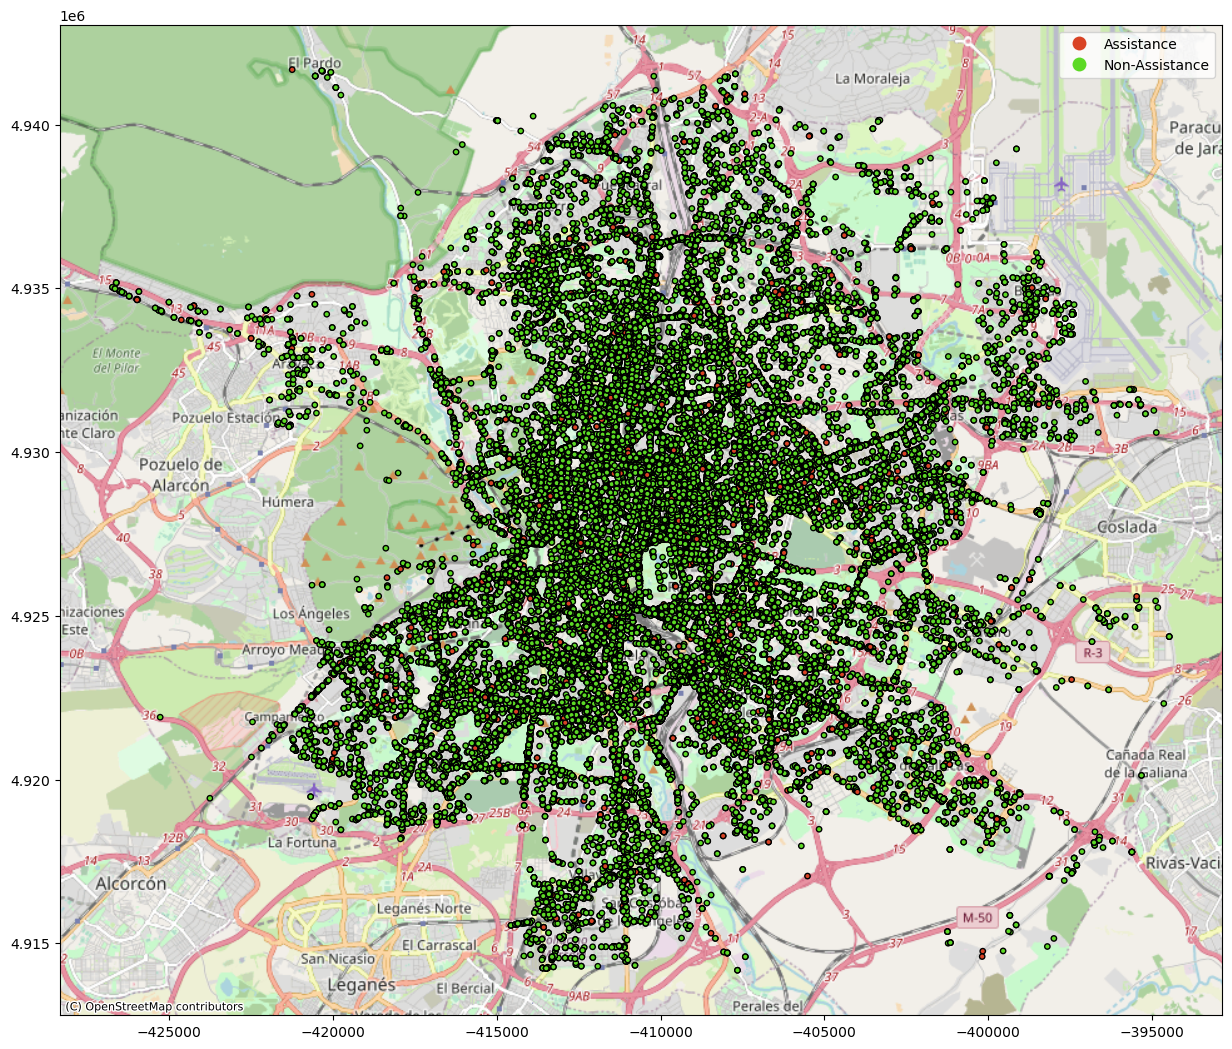
\includegraphics[width=75mm]{Figures/Madrid/original_OpenStreetMap.Mapnik.png}
        \label{MadridAccidentsMap:Original}
    }
    \subfigure[Madrid filtered accidents map.]{
        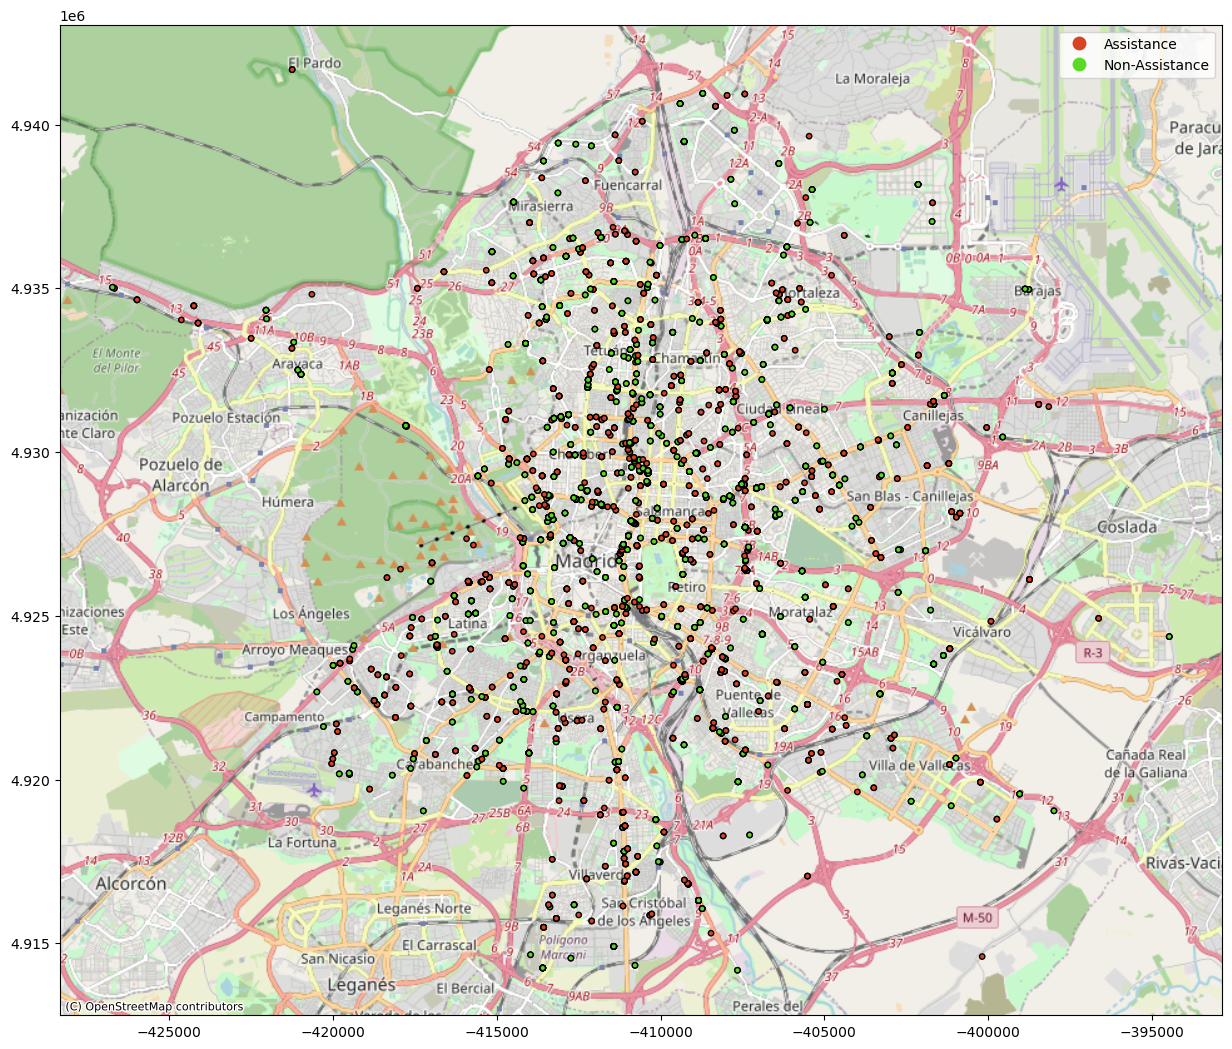
\includegraphics[width=75mm]{Figures/Madrid/filtered_OpenStreetMap.Mapnik.png}
        \label{MadridAccidentsMap:Filtered}
    }
    \caption{Madrid original/filtered accidents map.}
    \label{MadridAccidentsMap}
\end{figure}

En la Figura \ref{MadridLossFunction} se muestra la evolución de la función a optimziar (F1-Score) a lo largo de las 50 épocas para las que se ha entrenado el modelo GTAAF en la ciudad de Madrid. Se observa cómo el F1-Score para el conjunto de entrenamiento sufre una evolución importante durante las diez primeras épocas, después de las cuales sigue aumentando en menor medida. Por otra parte, la métrica sobre el conjunto de validación sufre una evolución más lenta, hasta aproximadamente la época 30 no se ve una clara evolución en la generalización del modelo sobre datos que nunca ha visto.


\begin{figure}[H]
\centering
    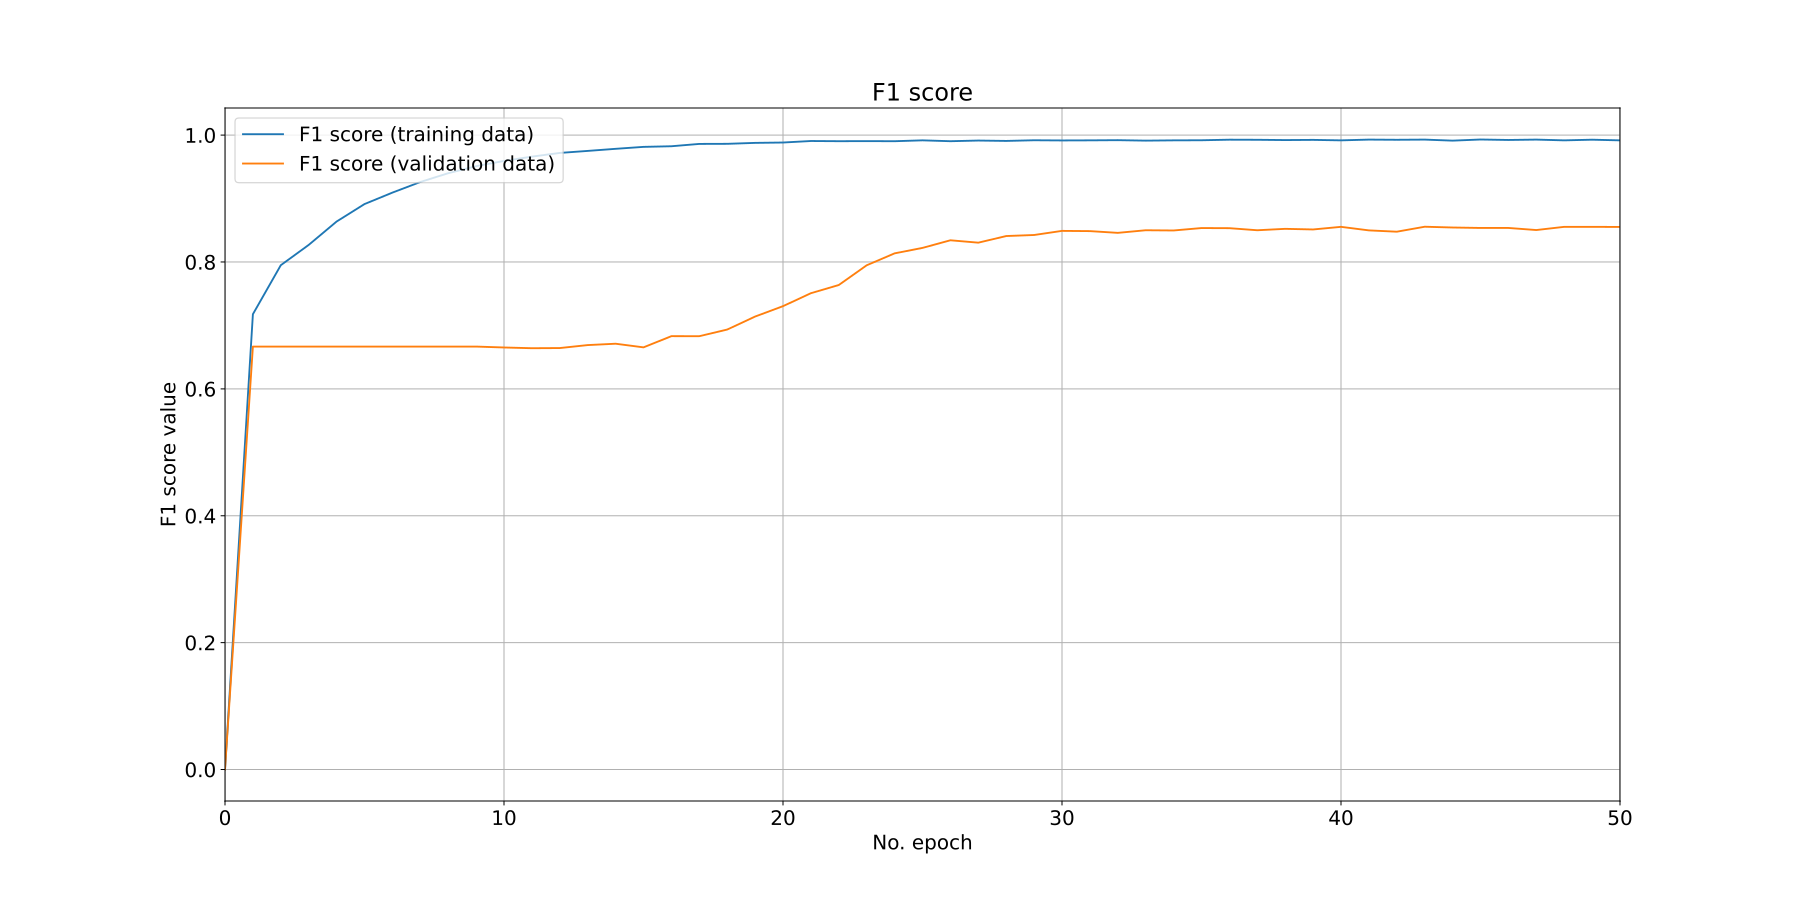
\includegraphics[width=160mm]{Figures/Madrid/madrid_convolution_2d_f1_score_2023-12-03-12 54 29.png}
    \caption{Evolution of F1-Score Madrid.}
\label{MadridLossFunction}
\end{figure}

En la tabla \ref{SpainMetrics} se observan los resultados de la métrica F1-Score de la predicción de la severidad de los accidentes de cada uno de los modelos sobre el conjunto de test de la ciudad de Madrid. Como se puede comprobar, el valor más alto lo ofrece el nuevo modelo GTAAF propuesto, llegando a mejorar en un 3,9\% al siguiente mejor modelo, el SVC sobre los accidentes Slight, mientras que la mejora sobre los accidentes Assistance se mide en un 5,7\% sobre el siguiente modelo que mejor métricas ofrece, el SVC. Con estos resultados puede interpretar que el nuevo modelo GTAAF propuesto es capaz de generalizar mejor en la predicción de la severidad de nuevos accidentes que no ha visto previamente sobre la ciudad de Madrid.

%%%%%%%%%%%%%%%%%%%%%%%%%%%%%%%%%%%%%%%%%%%%%%%%%%%%%%%%%%%%%%%%%%%%%%%%%%%%%%%%%
\begin{table}[H]
	\begin{center}
		\begin{tabular}{|c|c||c|c|c|c|c|c|}
		\hline
		\multicolumn{2}{ |c|| }{} &
		\multicolumn{1}{ |c| }{\textbf{Spain region F1-Score}} \\ \hline

		\textbf{Model} & \textbf{Assistance} & Madrid
		\\ \hline \hline

        \multirow{2}{*}{NB} &
            No &  0.729 \\ &
		    Yes & 0.621 \\ \hline \hline
        \multirow{2}{*}{SVC} &
            No & 0.862 \\ &
		    Yes &  0.748 \\ \hline \hline
        \multirow{2}{*}{KNN} &
            No  & 0.739 \\ &
            Yes & 0.634 \\ \hline \hline
        \multirow{2}{*}{RF} &
            No & 0.744 \\ &
            Yes & 0.643  \\ \hline \hline
        \multirow{2}{*}{LR} &
            No &  0.750 \\ &
            Yes & 0.623 \\ \hline \hline
        \multirow{2}{*}{MLP} &
            No & 0.856 \\ &
            Yes & 0.724  \\ \hline \hline
        \multirow{2}{*}{\textbf{GTAAF}} &
            \textbf{No} & \textbf{0.894} \\ &
            \textbf{Yes} & \textbf{0.798} \\ \hline \hline
		\end{tabular}
	\end{center}
	\caption{F1-Scores by Accident Class on Madrid (Spain).}
	\label{SpainMetrics}
\end{table}
%%%%%%%%%%%%%%%%%%%%%%%%%%%%%%%%%%%%%%%%%%%%%%%%%%%%%%%%%%%%%%%%%%%%%%%%%%%%%%%%%

En el segundo caso, tenemos una región dispersa, el estado de Victoria (Australia). Victoria, un estado en Australia, abarca una región diversa con ciudades bulliciosas como Melbourne, situada a lo largo de la costa sureste, conocida por su densidad de población moderada a alta y una mezcla de vitalidad urbana. En la figura \ref{VictoriaAccidentsMap} se muestra la distribución de accidentes sobre la población de Victoria, aquellos Non-Assistance se encuentran marcados en verde mientras que aquellos tipo Assistance se encuentran representados en rojo. Como se puede observar en la figura \ref{VictoriaAccidentsMap:Original} gran parte de la concentración de los accidentes se encuentra sobre la ciudad de Melbourne y sus núcleos urbanos próximos (como Ballarat al oeste, Shepparton al norte o Traralgon al este), al igual que en las carreteras que interconectan estas poblaciones. Al ser un estado extenso, el filtrado de áreas es más amplio, lo que resulta una variante respecto a ciudades de mayor concentración. En la Figura \ref{VictoriaAccidentsMap:Filtered} se observa la distribución de accidentes resultante tras aplicar el proceso de filtrado, donde aquellas zonas que presentan más accidentes necesarios de asistencia son en las grandes poblaciones y en las interconexiones entre estas.


 \begin{figure}[H]
     \centering
     \subfigure[Victoria original accidents map.]{
         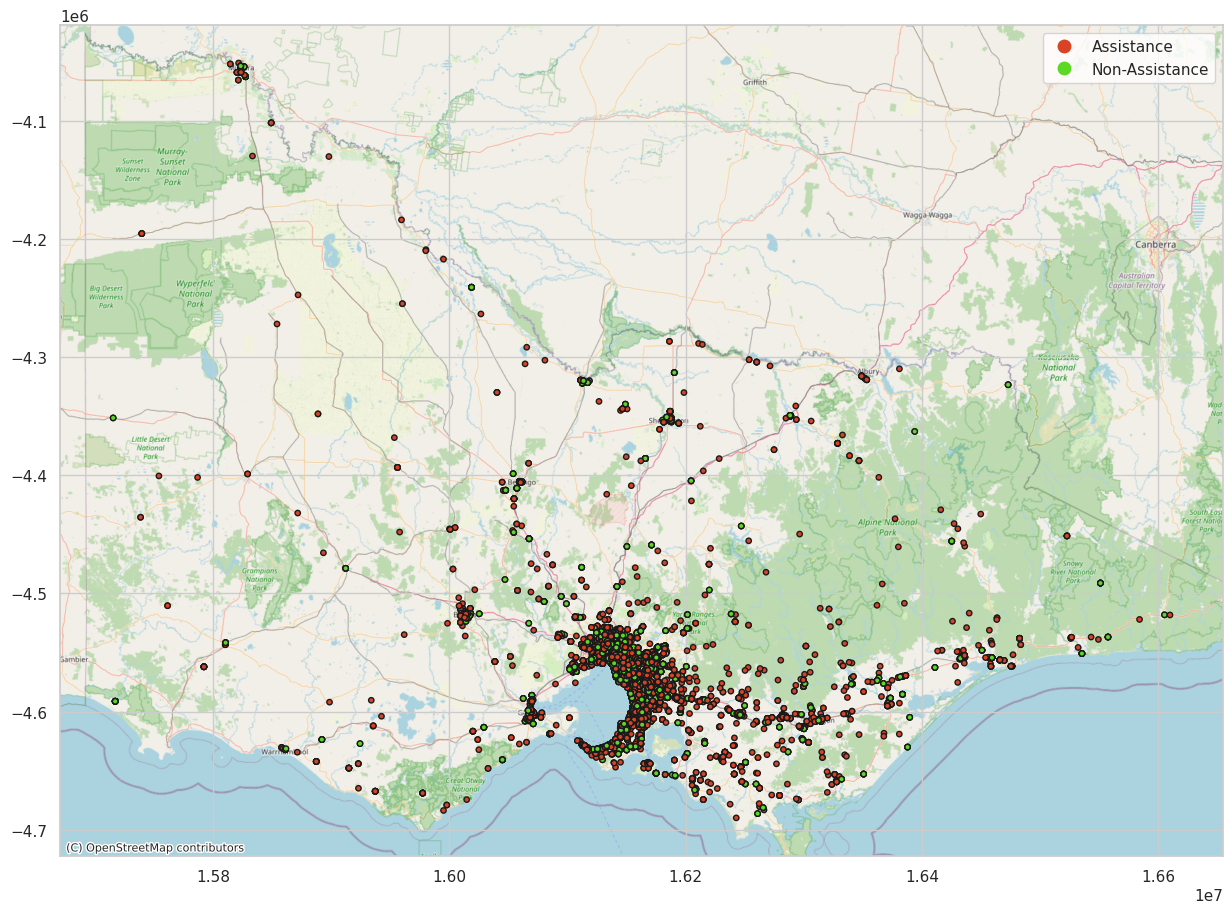
\includegraphics[width=75mm]{Figures/Victoria/original_OpenStreetMap.Mapnik.png}
         \label{VictoriaAccidentsMap:Original}
     }
     \subfigure[Victoria filtered accidents map.]{
         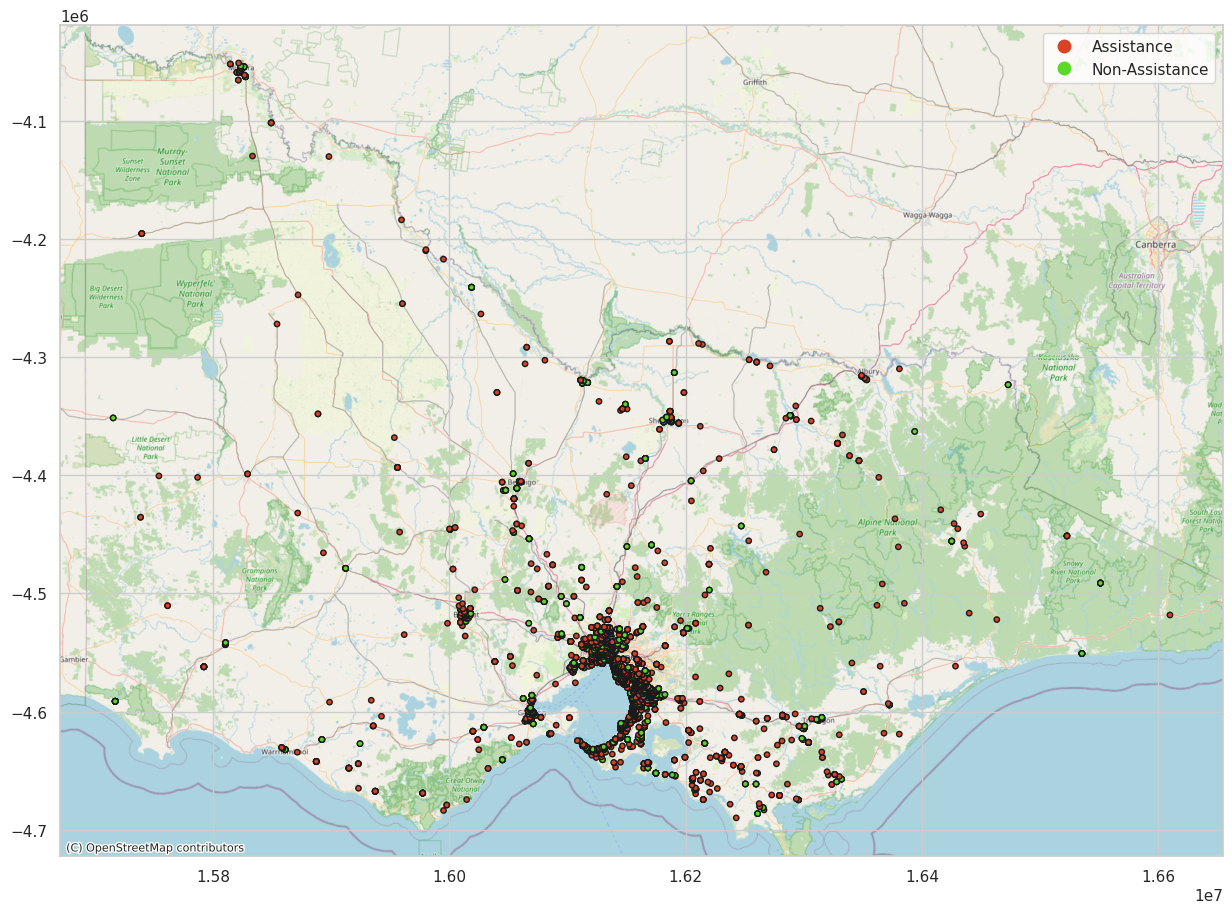
\includegraphics[width=75mm]{Figures/Victoria/filtered_OpenStreetMap.Mapnik.png}
         \label{VictoriaAccidentsMap:Filtered}
     }
     \caption{Victoria original/filtered accidents map.}
     \label{VictoriaAccidentsMap}
 \end{figure}


En la Figura \ref{VictoriaLossFunction} se muestran las funciones F1-Score sobre los datos de entrenamineto y validación para la región de Victoria. Esta métrica sobre el conjunto de entrenamiento muestra una curva de aprendizaje más lenta respecto a la ciudad de Madrid, lo cual es comprensible ya que existe más variabilidad de datos en esta región al ser mucho más extensa que la anterior. La función de validación presenta más variaciones a lo largo del aprendizaje, llegando a su máximo aproximadamente en la época 45.

\begin{figure}[H]
\centering
    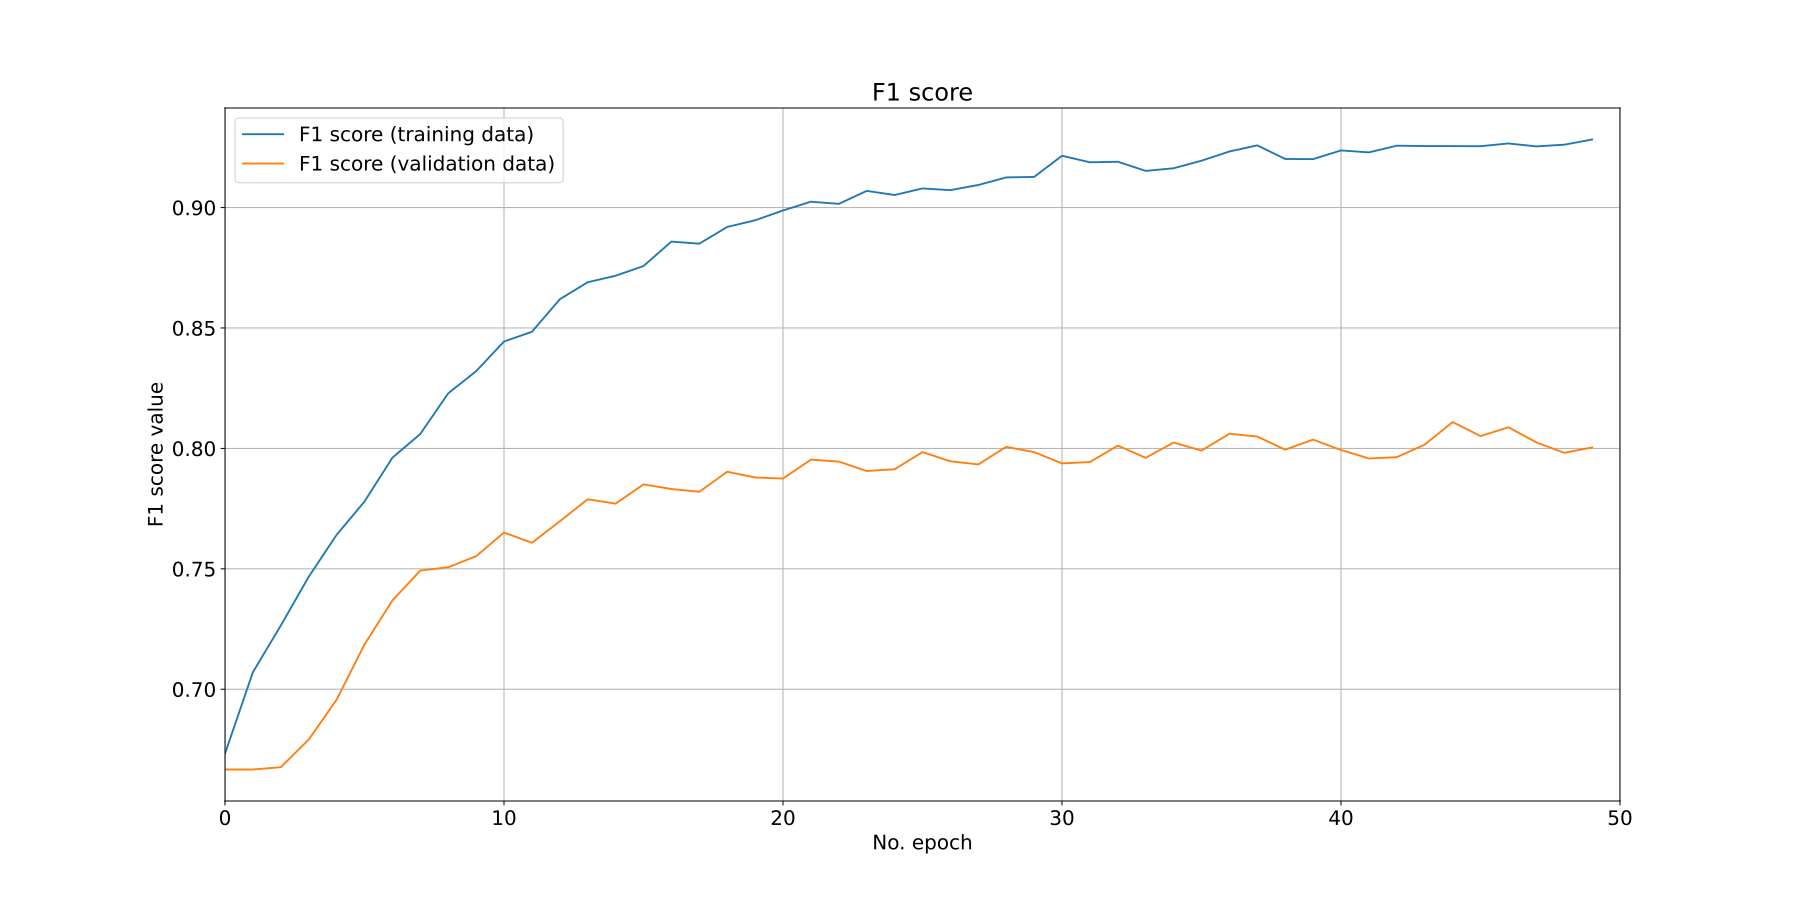
\includegraphics[width=160mm]{Figures/Victoria/Victoria_convolution_2d_f1_score_paper.png}
    \caption{Evolution of F1-Score Victoria.}
\label{VictoriaLossFunction}
\end{figure}

En la Tabla \ref{AustraliaMetrics}, se presentan los resultados del F1-Score obtenidos por cada uno de los modelos para ambos tipos de clasificación de accidentes. Específicamente, se observa que para la población de Victoria, el nuevo modelo GTAAF propuesto logra una mejora del 6.5\% en comparación con el siguiente mejor modelo, el SVC, para accidentes de No Asistencia. Por otro lado, en lo que respecta a accidentes de tipo Asistencia, hay una mejora del 9\% en comparación con el MLP. Estos resultados reflejan una mejora significativa en la capacidad de generalización del nuevo modelo propuesto.

%%%%%%%%%%%%%%%%%%%%%%%%%%%%%%%%%%%%%%%%%%%%%%%%%%%%%%%%%%%%%%%%%%%%%%%%%%%%%%%%%
\begin{table}[H]
	\begin{center}
		\begin{tabular}{|c|c||c|c|c|c|c|c|}
		\hline
		\multicolumn{2}{ |c|| }{} &
		\multicolumn{1}{ |c| }{\textbf{Australia region F1-Score}} \\ \hline

		\textbf{Model} & \textbf{Assistance} & Victoria
		\\ \hline \hline

        \multirow{2}{*}{NB} &
            No &  0.635 \\ &
		    Yes & 0.476 \\ \hline \hline
        \multirow{2}{*}{SVC} &
            No & 0.662 \\ &
		    Yes &  0.679 \\ \hline \hline
        \multirow{2}{*}{KNN} &
            No  & 0.654 \\ &
            Yes & 0.616 \\ \hline \hline
        \multirow{2}{*}{RF} &
            No & 0.647 \\ &
            Yes & 0.364  \\ \hline \hline
        \multirow{2}{*}{LR} &
            No &  0.612 \\ &
            Yes & 0.630 \\ \hline \hline
        \multirow{2}{*}{MLP} &
            No & 0.635 \\ &
            Yes & 0.694 \\ \hline \hline
        \multirow{2}{*}{\textbf{GTAAF}} &
            \textbf{No} & \textbf{0.727} \\ &
            \textbf{Yes} & \textbf{0.784} \\ \hline \hline
		\end{tabular}
	\end{center}
	\caption{F1-Scores by Accident Class on Victoria (Australia).}
	\label{AustraliaMetrics}
\end{table}
%%%%%%%%%%%%%%%%%%%%%%%%%%%%%%%%%%%%%%%%%%%%%%%%%%%%%%%%%%%%%%%%%%%%%%%%%%%%%%%%%

En la Tabla \ref{AustraliaMetrics} se muestran los resultados F1-Score obtenidos de cada uno de los modelos respecto a ambos tipos de clasificación de accidentes. Concretamente se observa que para la ciudad de Victoria el nuevo modelo GTAAF propuesto obtiene una mejora respecto al siguiente mejor modelo, el SVC, para los accidentes Slight del 6,5\%. Por otra parte, en lo que respecta a los accidentes tipo Assistance se obtiene una mejora del 9\% respecto al MLP. Estos resultados reflejan una mejora de generaliación significativa del nuevo modelo propuesto.



\textbf{Southwark}\\

Southwark es un distrito de Londres situado en la orilla sur del río Támesis, con una alta densidad de población. En la Figura \ref{SouthwarkAccidentsMap} se observa la distribución de los accidentes a lo largo del municipio de Southwark. Analizando los accidentes del conjunto de datos original, Figura \ref{SouthwarkAccidentsMap:Original}, se observa que estos se producen a lo largo de las distintas vías que conectan el municipio con el centro neurálgico de la ciudad, hecho habitual al conectar zonas menos pobladas con lugars de trabajo y de ocio, mientras que la minoría de ellos se presentan en las calles aledañas. Observando la distribución de accidentes tras el proceso de filtrado por áreas (Figura \ref{SouthwarkAccidentsMap:Filtered}) se acentúa este hecho, donde se observan que aquellos principales accidentes Assistance se producen en estas vías. Por otra parte se muestra una concentracion minoritaria de este tipo de accidentes en la zona de Dulwich (sur), en la intersección de la circunvalación S Circular red con la carretera que dirige al centro del municipio.


 \begin{figure}[H]
     \centering
     \subfigure[Southwark original accidents map.]{
         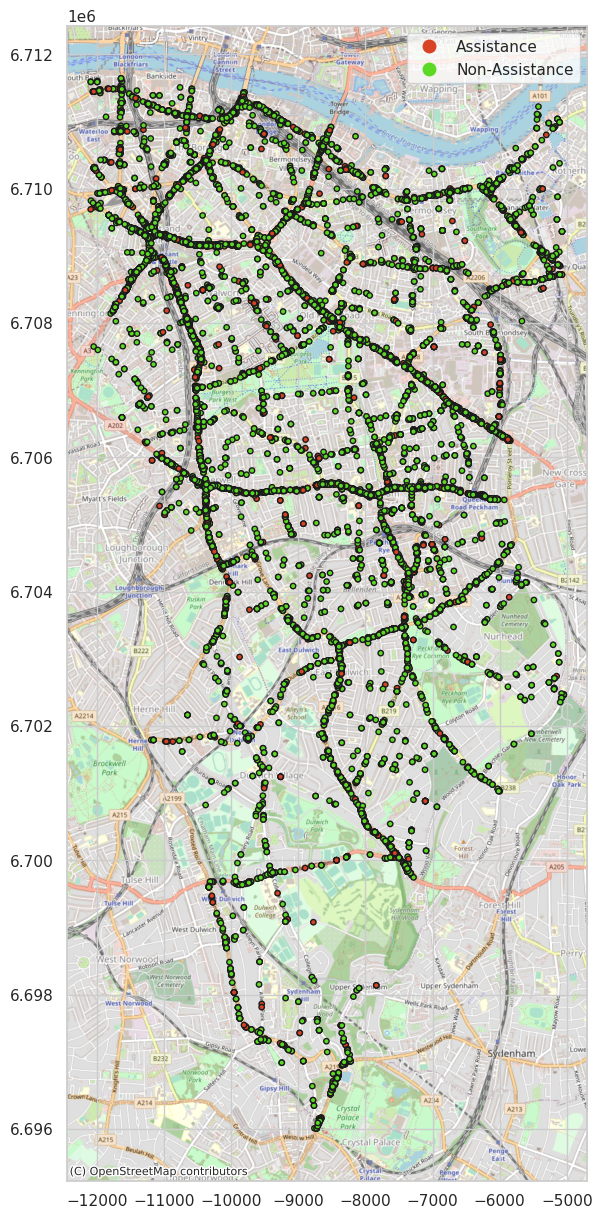
\includegraphics[width=75mm]{Figures/Southwark/original_OpenStreetMap.Mapnik.png}
         \label{SouthwarkAccidentsMap:Original}
     }
     \subfigure[Southwark filtered accidents map.]{
         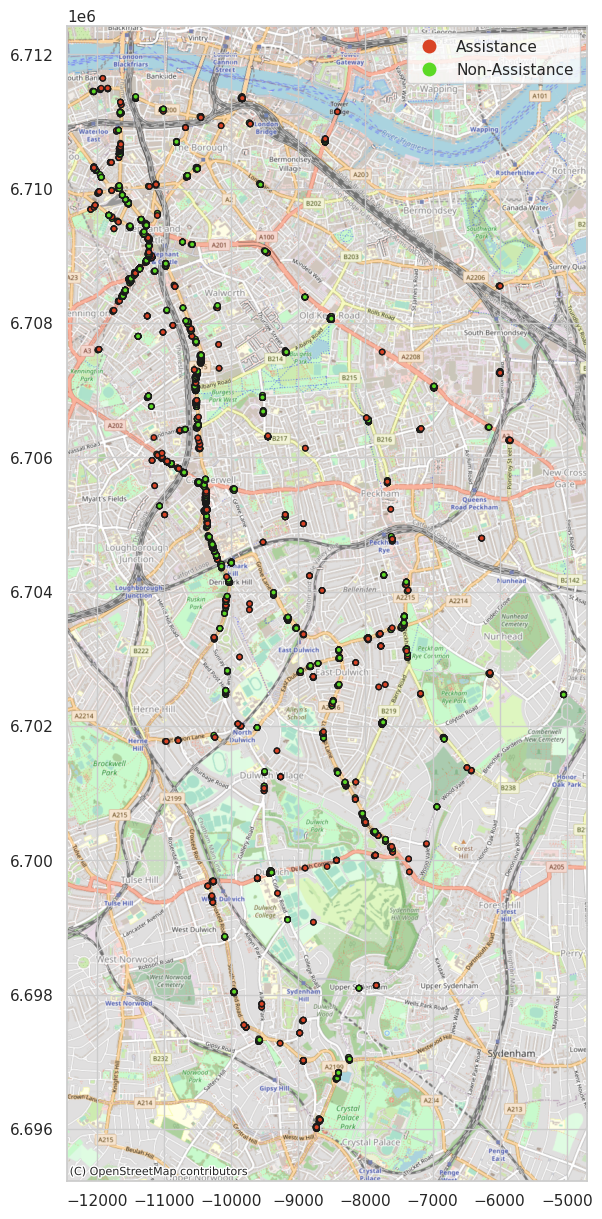
\includegraphics[width=75mm]{Figures/Southwark/filtered_OpenStreetMap.Mapnik.png}
         \label{SouthwarkAccidentsMap:Filtered}
     }
     \caption{Southwark original/filtered accidents map.}
     \label{SouthwarkAccidentsMap}
 \end{figure}


\textbf{Manchester}\\

Manchester, ubicada en el noroeste de Inglaterra, es una gran ciudad conocida por su legado industrial y su alta densidad de población. En la Figure \ref{ManchesterAccidentsMap} se muestra la distribución de los accidentes de Manchester. Atendiendo a la distribución de accidentes original, en la Figura \ref{Manchester:Original}, como es habitual en cualquier población se aprecia una concentración de accidentes imrpotante en la zona central de la ciudad, siendo también considerable en el área de Longsight. Por otra parte, las principales vías que comunican las perifieras urbanas (norte) con el centro de la ciudad también presentan una concentración mayor de accidentes, lo que puede deberse a desplazamientos por trabajo. Por otra parte, la carretera de Wythenshawe, cercano a Sale Water Park (Sur), también presenta una concentración elevada de accidentes, motivados por los desplazamientos de ocio y de trabajo. En la figura \ref{ManchesterAccidentsMap:Filtered} se observa la localización de los accidentes una vez se ha aplicado el proceso de filtrado por áreas, donde se vislumbra que gran parte de los accidentes Assistance se distribuyen a lo largo de las carreteras que comunican hacia el centro de la ciudad.


 \begin{figure}[H]
     \centering
     \subfigure[Manchester original accidents map.]{
         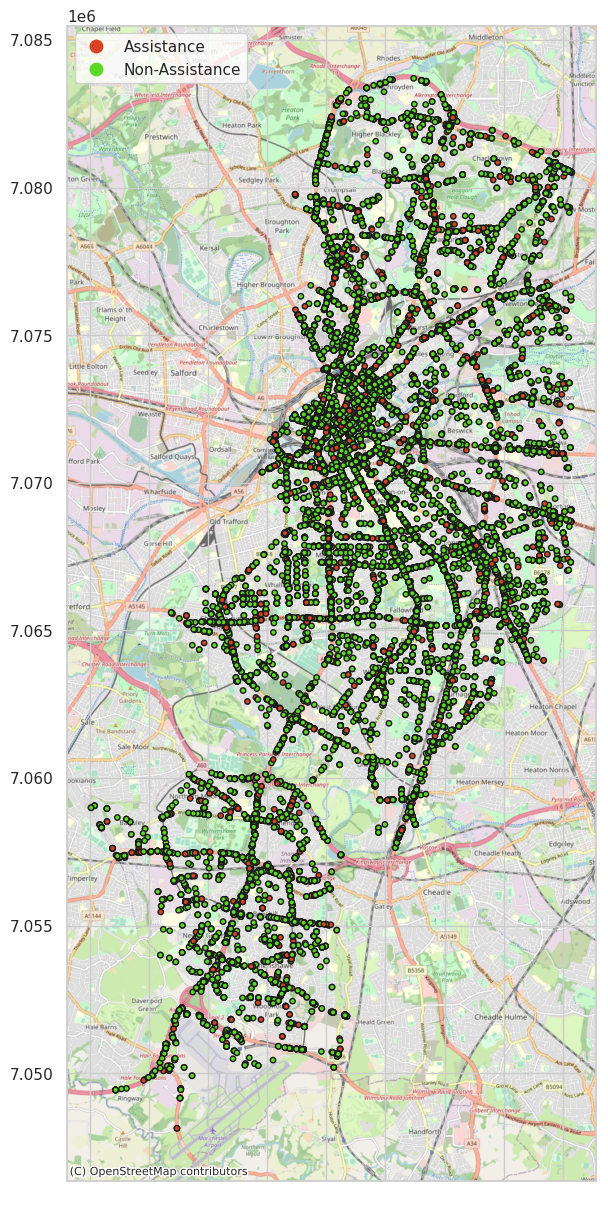
\includegraphics[width=75mm]{Figures/Manchester/original_OpenStreetMap.Mapnik.png}
         \label{ManchesterAccidentsMap:Original}
     }
     \subfigure[Manchester filtered accidents map.]{
         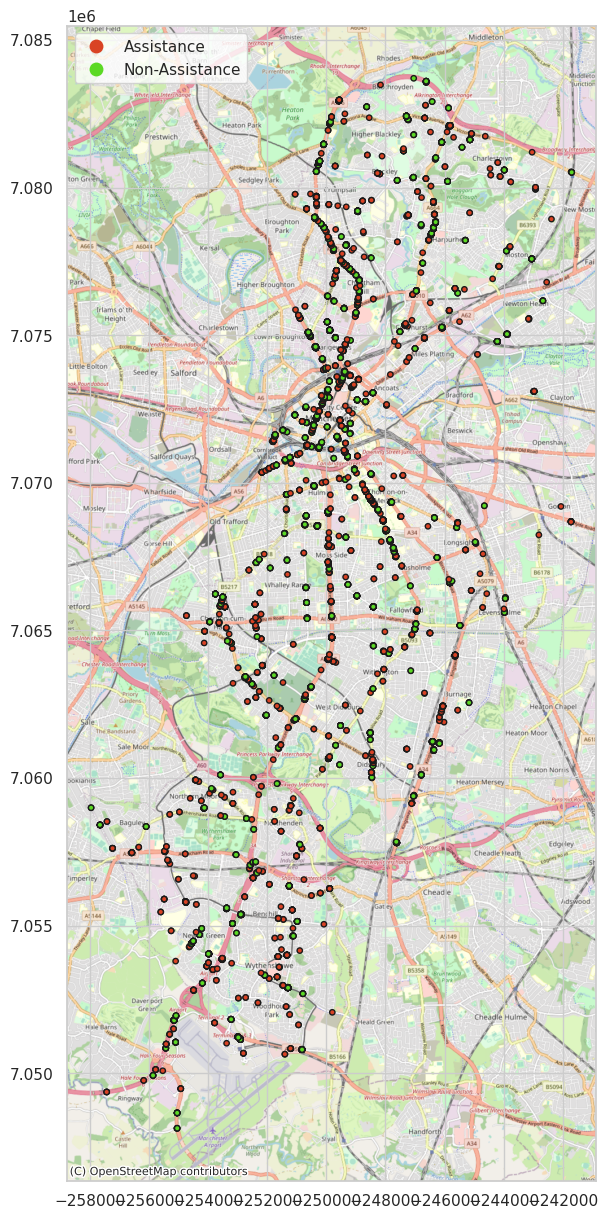
\includegraphics[width=75mm]{Figures/Manchester/filtered_OpenStreetMap.Mapnik.png}
         \label{ManchesterAccidentsMap:Filtered}
     }
     \caption{Manchester original/filtered accidents map.}
     \label{ManchesterAccidentsMap}
 \end{figure}

\textbf{Birmingham}\\

Birmingham, la segunda ciudad más grande de Inglaterra, se extiende por West Midlands con un paisaje urbano diverso y una densidad de población considerable, famosa por su historia industrial y su vitalidad cultural. En la Figura \ref{BirminghamAccidentsMap} se muestra la distribución de los accidentes de Birmingham, tanto los originales como los resultantes una vez aplicado el proceso de filtrado. Como se puede observar en los accidentes originales en la Figura \ref{BirminghamAccidentsMap:Original} se aprecia que gran parte de los accidentes se concentran en la zona centro de la ciudad, una  tendencia normal debido a que es el principal foco de actividad de las ciudades. Mientras que los accidentes se van dispersando a medida que distan de este punto. Se aprecian ligeras agrupaciones de accidentes a lo largo de las zonas de incorporaciones a las principales arterias de la ciudad, como es al este, el caos de Handsworth. Por otra parte, en la figura \ref{BirminghamAccidentsMap:Filtered} se muestran los accidentes una vez se ha aplicado el proceso de filtrado por áreas. Como se peude observar, la información ha sido resumida sin dar lugar a pérdidas en el valor de la misma. Se vislumbran ciertas zonas más conflictivas donde se producen accidentes más importantes, como es el caso de la carretera Holyhead Rd de entrada a la ciudad o en Northfield.

 \begin{figure}[H]
     \centering
     \subfigure[Birmingham original accidents map.]{
         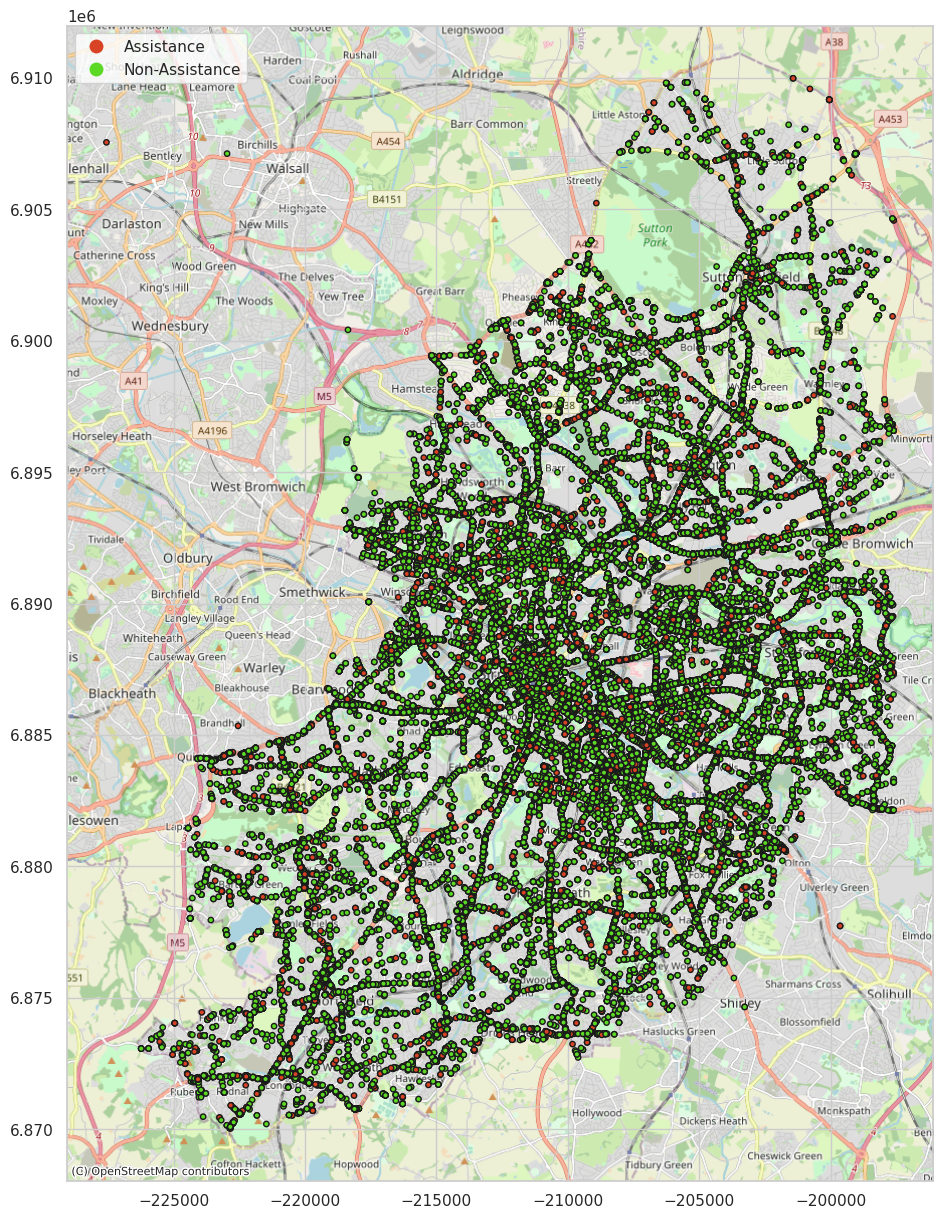
\includegraphics[width=75mm]{Figures/Birmingham/original_OpenStreetMap.Mapnik.png}
             \label{BirminghamAccidentsMap:Original}
     }
     \subfigure[Birmingham filtered accidents map.]{
         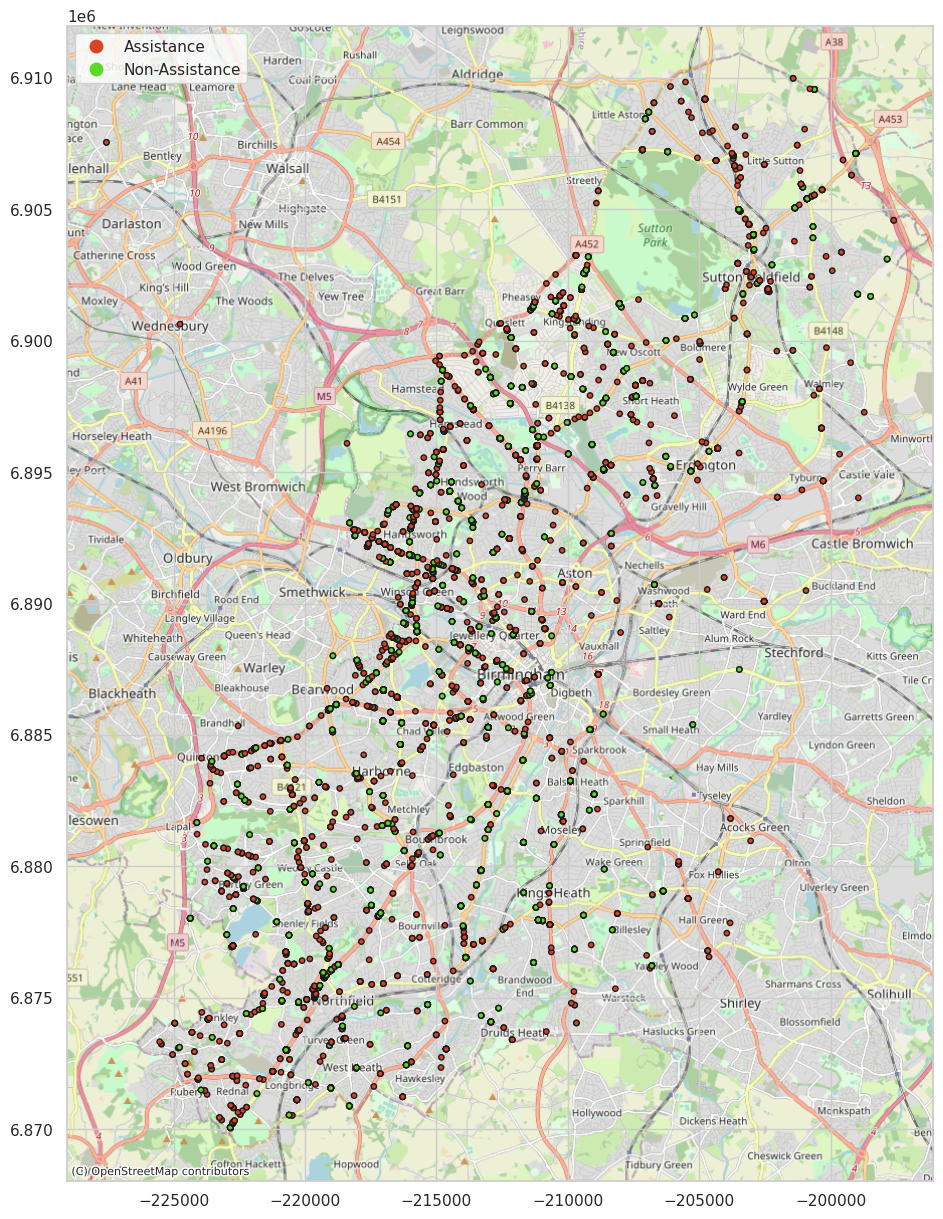
\includegraphics[width=75mm]{Figures/Birmingham/filtered_OpenStreetMap.Mapnik.png}
         \label{BirminghamAccidentsMap:Filtered}
     }
     \caption{Birmingham original/filtered accidents map.}
     \label{BirminghamAccidentsMap}
 \end{figure}


\textbf{Liverpool}\\

Liverpool, ubicada a lo largo del río Mersey en el noroeste de Inglaterra, prospera como una ciudad marítima con una rica historia, profundidad cultural y una densidad de población significativa, reconocida por su encanto en el frente marítimo y su legado musical. En la Figura \ref{LiverpoolAccidentsMap} se muestra la comparativa de la distribución de accidentes originales del dataset y filtrados para la ciudad de Liverpool. En la Figura \ref{LiverpoolAccidentsMap:Original} se aprecian accidentes concentrados en la zona centro de la ciudad, como viene siendo habitual, además de a lo largo de las circunvalaciones que la rodean. En la Figura \ref{LiverpoolAccidentsMap:Filtered}, después del proceso de filtrado, se aprecia que gran parte de los accidentes Assistance se producen a lo largo de Strand Street (desde el sur hasta el oeste), convergiendo ambas direcciones en el centro neuralgico. Por otra parte se visualiza otra concentración en la carretera que conecta la localidad de Ormskirk con el centro (noroeste), una de las principales vías de conexión.


 \begin{figure}[H]
     \centering
     \subfigure[Liverpool original accidents map.]{
         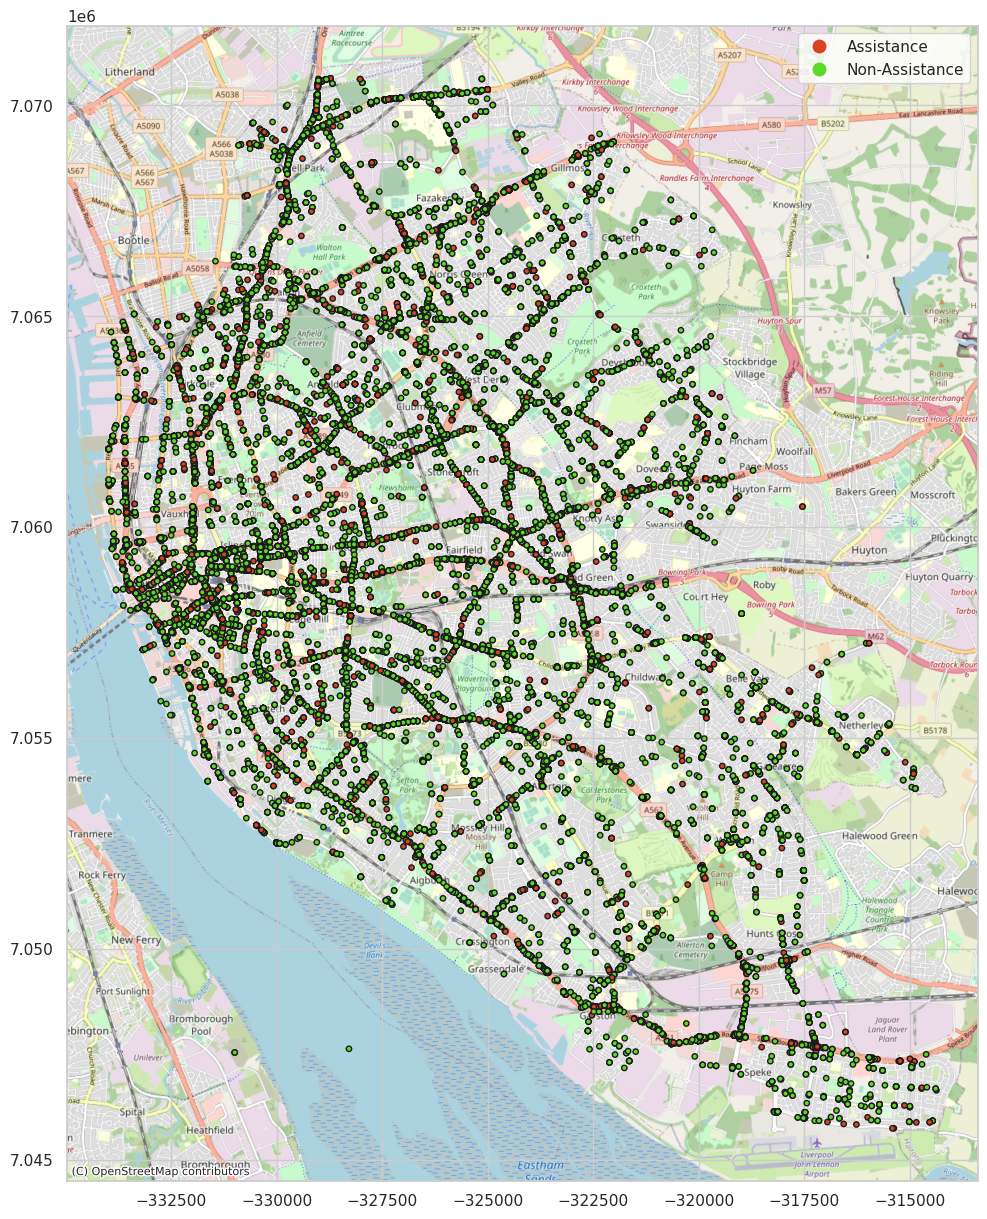
\includegraphics[width=75mm]{Figures/Liverpool/original_OpenStreetMap.Mapnik.png}
         \label{LiverpoolAccidentsMap:Original}
     }
     \subfigure[Liverpool filtered accidents map.]{
         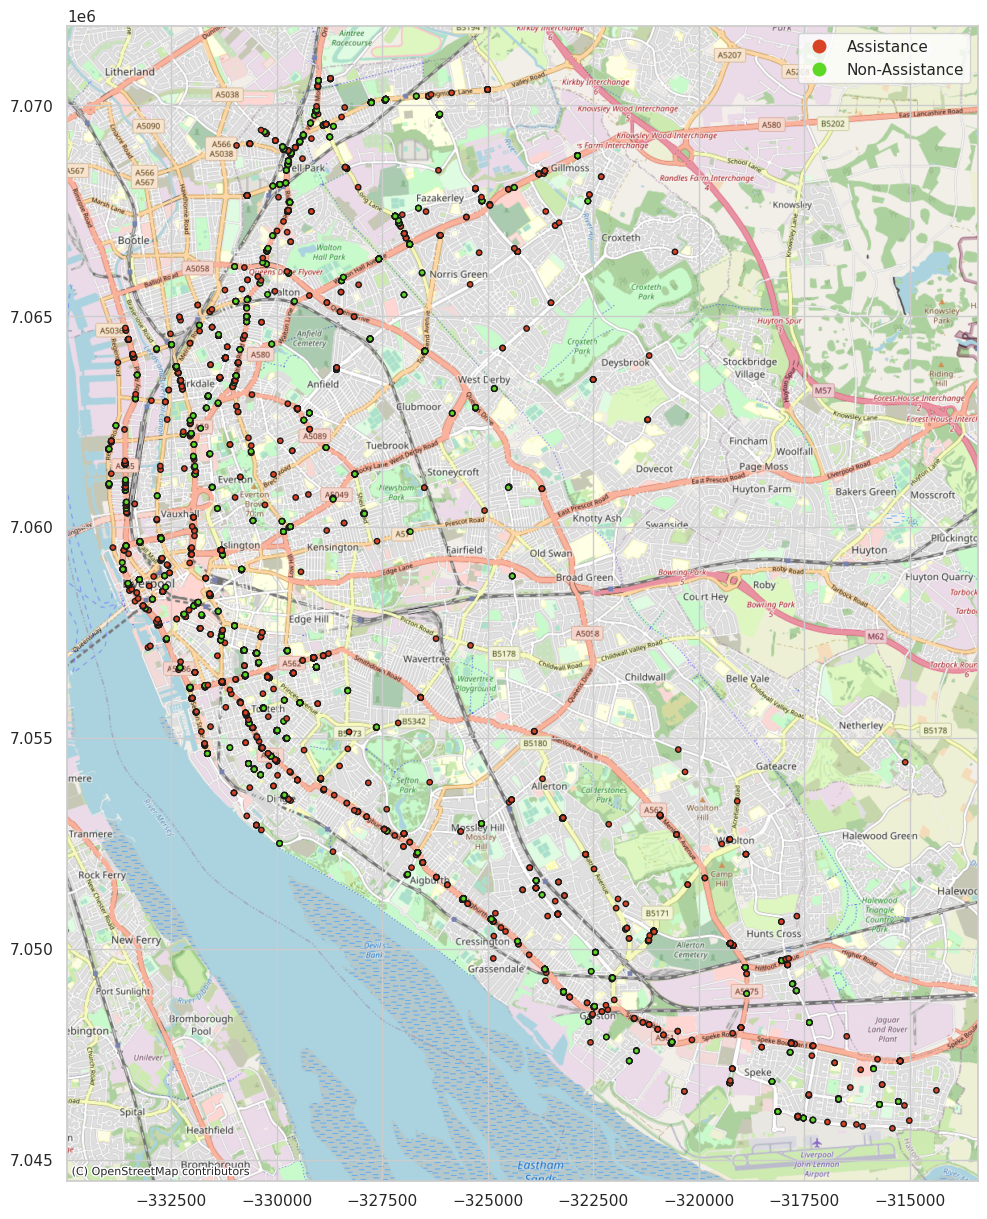
\includegraphics[width=75mm]{Figures/Liverpool/filtered_OpenStreetMap.Mapnik.png}
         \label{LiverpoolAccidentsMap:Filtered}
     }
     \caption{Liverpool original/filtered accidents map.}
     \label{LiverpoolAccidentsMap}
 \end{figure}

\textbf{Sheffield}\\

Sheffield, ubicada en South Yorkshire, presume de un patrimonio industrial y paisajes pintorescos, con una densidad de población intermedia. En la Figura \ref{SheffieldAccidentsMap} se muestra la distribución de accidentes para la ciudad de Sheffield, tanto la original como la resultante tras la etapa de filtrado. En la Figura \ref{SheffieldAccidentsMap:Original} se pueden apreciar distintas concentraciones en zonas estratégicas. Como suele ser habitual, el núcleo urbano es un centro de mayor densidad de incidenentes, mientras que en las intersecciones que conectan la ciudad de Sheffield y la de Rotherham (cruces de Tinsley Viaduct con Meadow Bank Road y la A6178, al noreste de Sheffield). También se aprecian concentraciones en los suburbios de Wadsley Bridge y Malin Bridge, periferias de la ciudad, además de alrededor de todas las vías principales que conectan con el centro. Por otra parte, en la figura \ref{SheffieldAccidentsMap:Filtered} se muestran los accidentes una vez se ha realizado el proceso de filtrado, donde se aprecia que aquellos que han requerido de asistencia normalemente se presentan en las principales arterias, donde se circula a una mayor velocidad.

 \begin{figure}[H]
     \centering
     \subfigure[Sheffield original accidents map.]{
         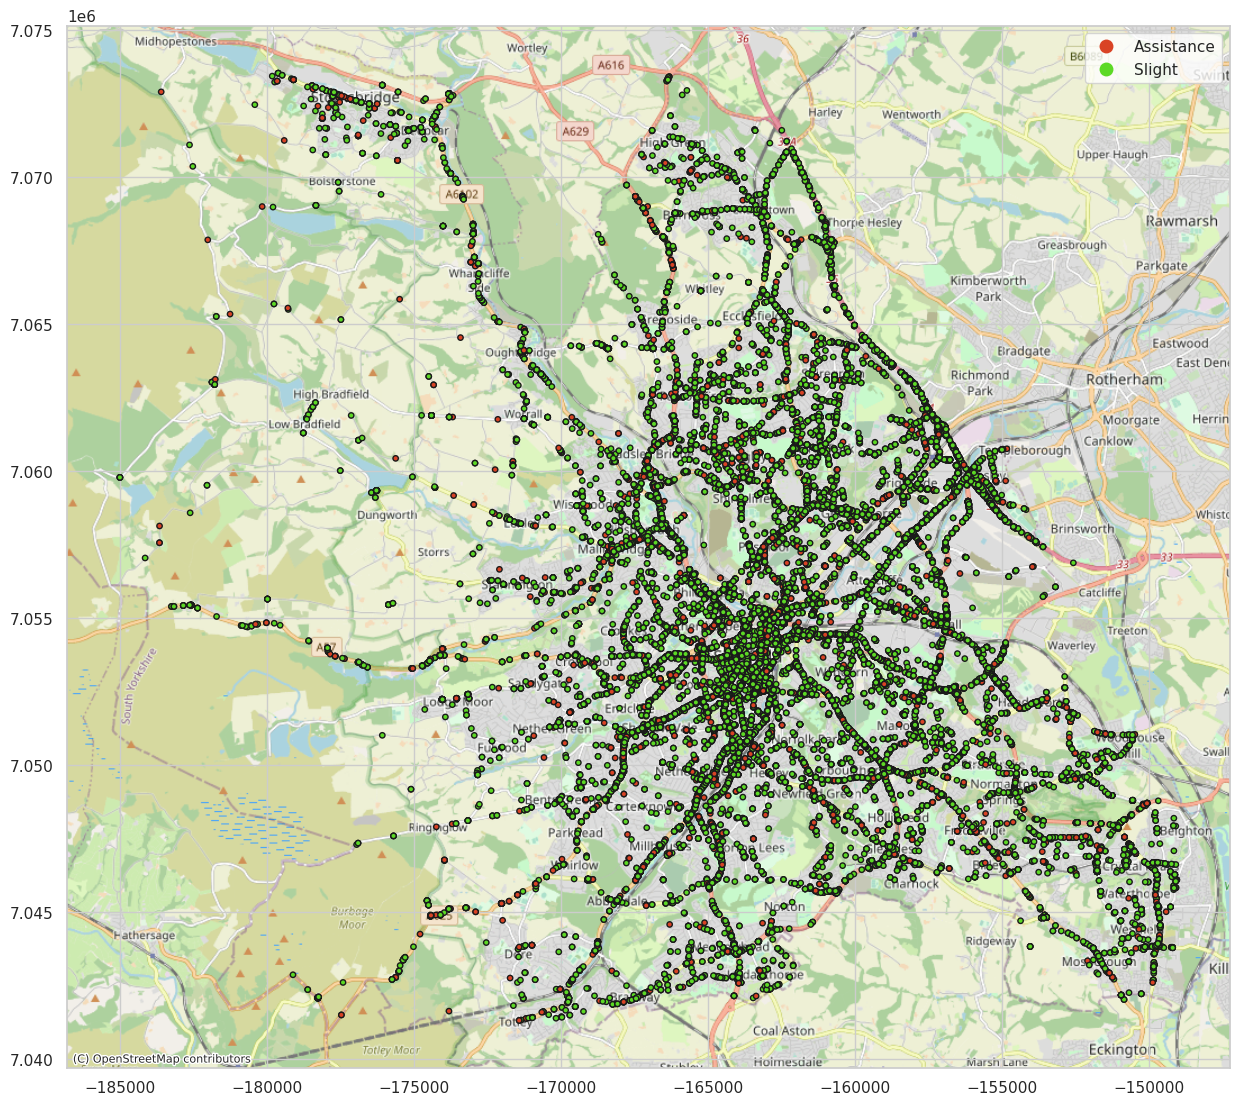
\includegraphics[width=75mm]{Figures/Sheffield/original_OpenStreetMap.Mapnik.png}
         \label{SheffieldAccidentsMap:Original}
     }
     \subfigure[Sheffield filtered accidents map.]{
         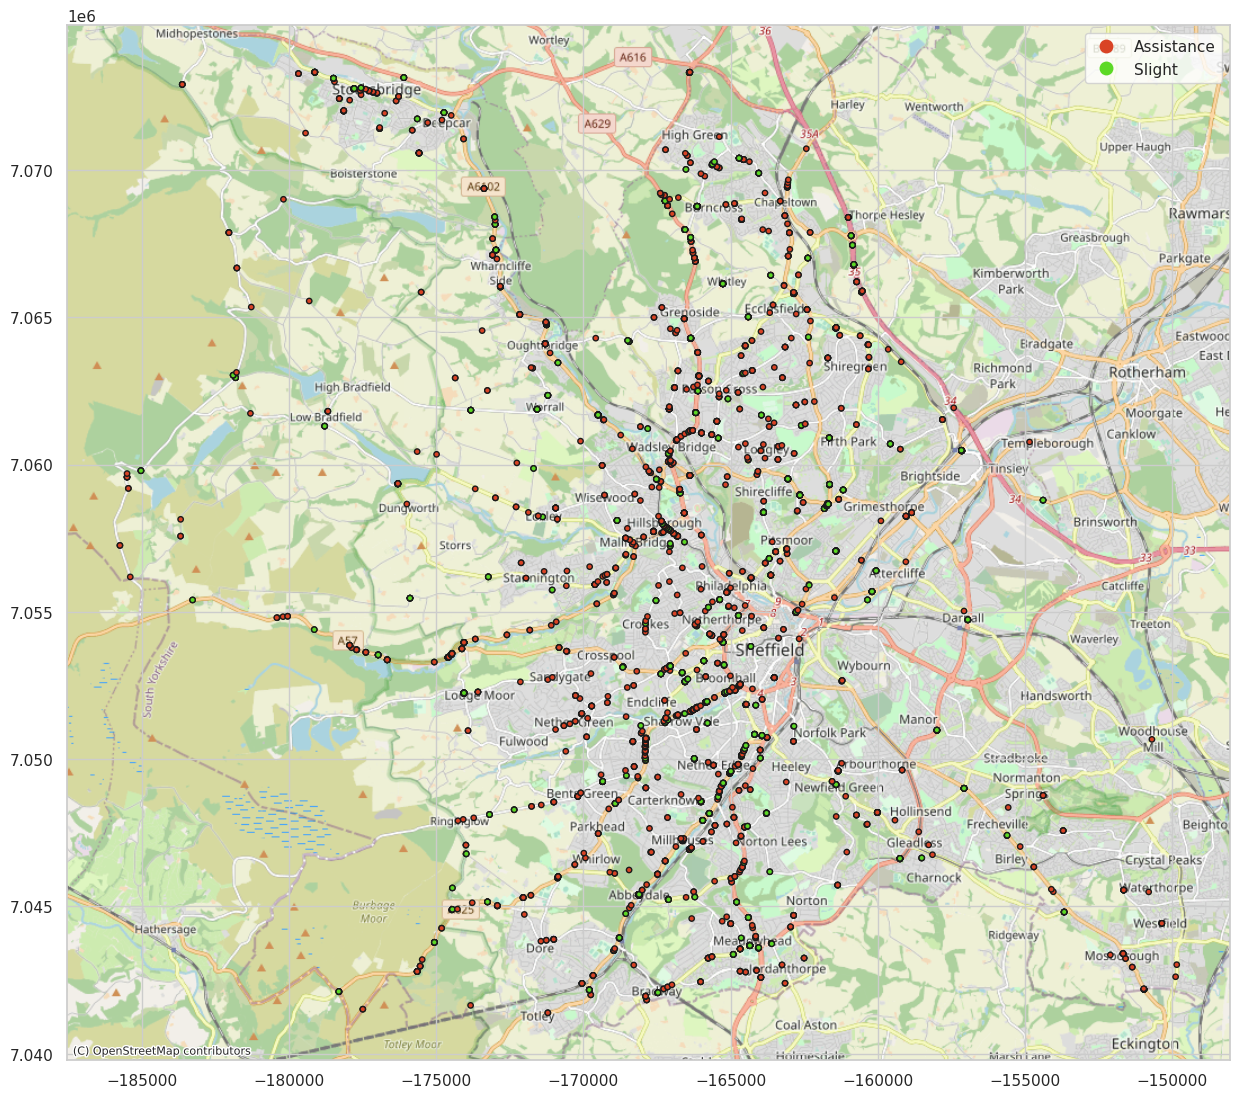
\includegraphics[width=75mm]{Figures/Sheffield/filtered_OpenStreetMap.Mapnik.png}
         \label{SheffieldAccidentsMap:Filtered}
     }
     \caption{Sheffield original/filtered accidents map.}
     \label{SheffieldAccidentsMap}
 \end{figure}


\textbf{Cornwall}\\

Cornualles, situada en la parte suroeste de Inglaterra con sus apacibles paisajes, encantadores pueblos costeros y extensiones rurales, fomenta un entorno tranquilo alejado de los núcleos de alta densidad de población. En la Figura \ref{CornwallAccidentsMap} se muestran de nuevo los accidentes originales de dataset y los que resultan tras aplicar el proceso de filtrado sobre el condado de Cornwall. En la Figura \ref{CornwallAccidentsMap:Original} las principales concentraciones de accidentes se encuentran distribuídas a lo largo de las distintas ciudades del condado. La mayoría de estos se encuentran dividios en dos regiones claramente definidas, la primera de ellas entre las vías que conectan las localidades de Camborne y Redruth (suroeste de Cornwall), y el área comprendida entre St Austell, Duporth, Carlyon Bay y Par, este del condado. No obstante, el resto de regiones también presentan una concentración considerable, como es el caso de la ciudad de Falmouth (sureste), las localidades de Penzance y Hayle (suroeste), en la ciudad de Newquay y sus alrededores (oeste), Bodmin (centro) y Launceston (norte). De nuevo, en este caso, se demuestra que la mayor frecuencia de accidentes se presenta entre los principales núcleos de población y las carreteras que los interconectan, debido a que las grandes ciudades implican más movimientos de vehículos. Atendiendo a la Figura \ref{CornwallAccidentsMap:Filtered} se observa que la ocurrencia de accidentes necesarios de asistencia, una vez aplicado el proceso de filtrado, tiene la misma tendencia que el expuesto para el conjunto de datos original, distribuyéndose a lo largo de las principales carreteras del condado Cornwall y concentrándose más en los núcleos de población.


 \begin{figure}[H]
     \centering
     \subfigure[Cornwall original accidents map.]{
         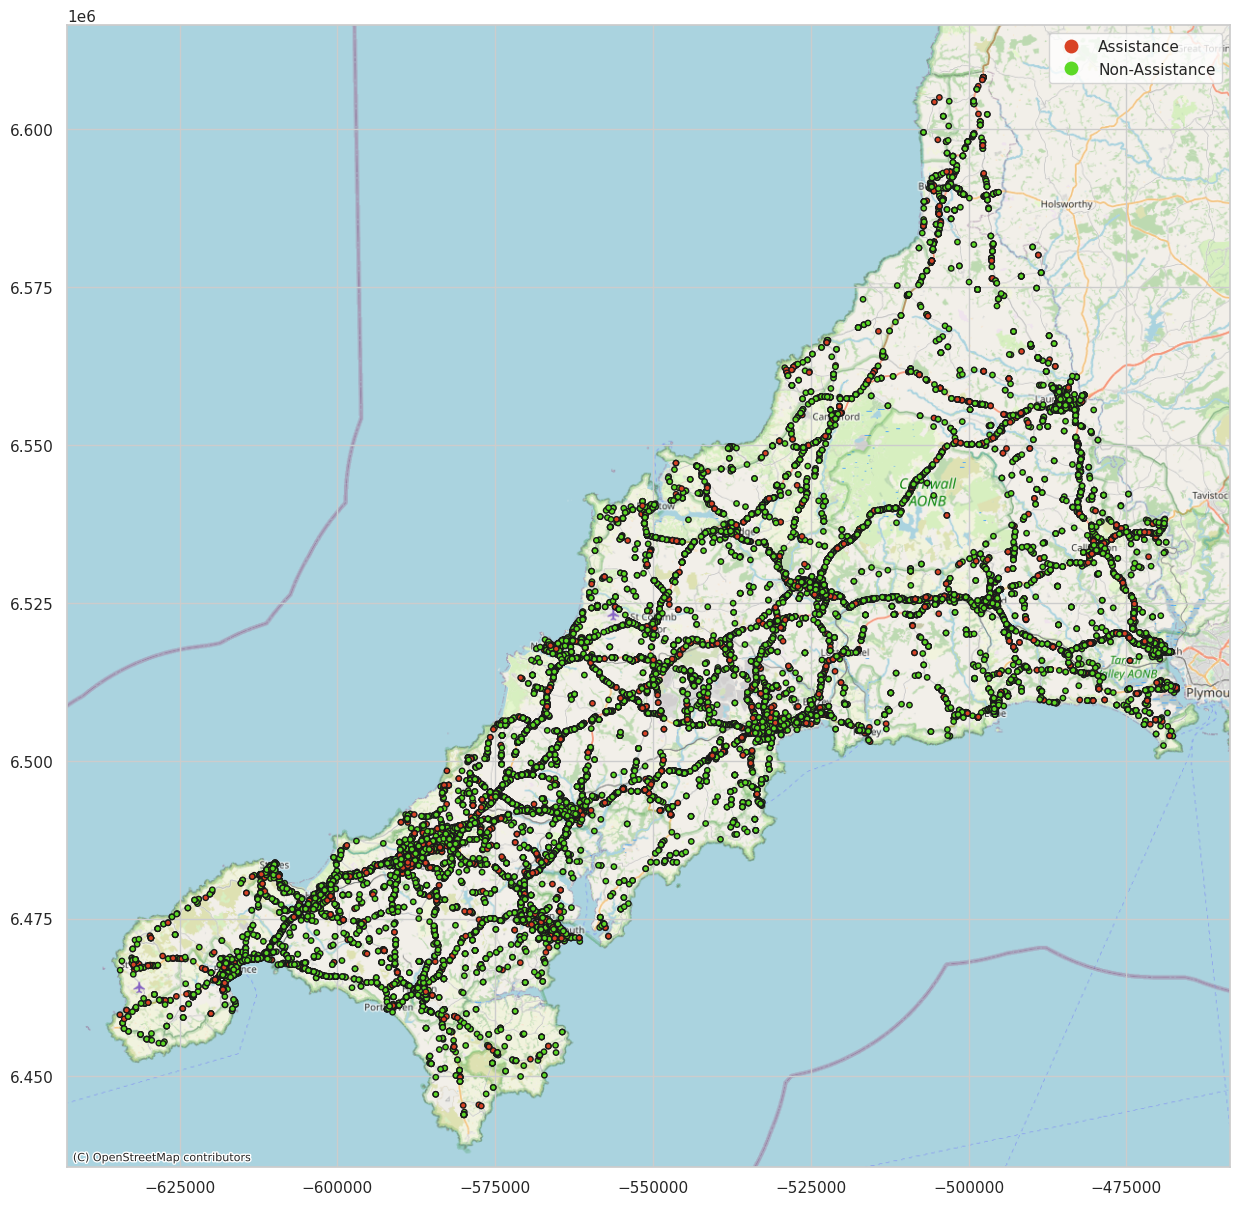
\includegraphics[width=75mm]{Figures/Cornwall/original_OpenStreetMap.Mapnik.png}
         \label{CornwallAccidentsMap:Original}
     }
     \subfigure[Cornwall filtered accidents map.]{
         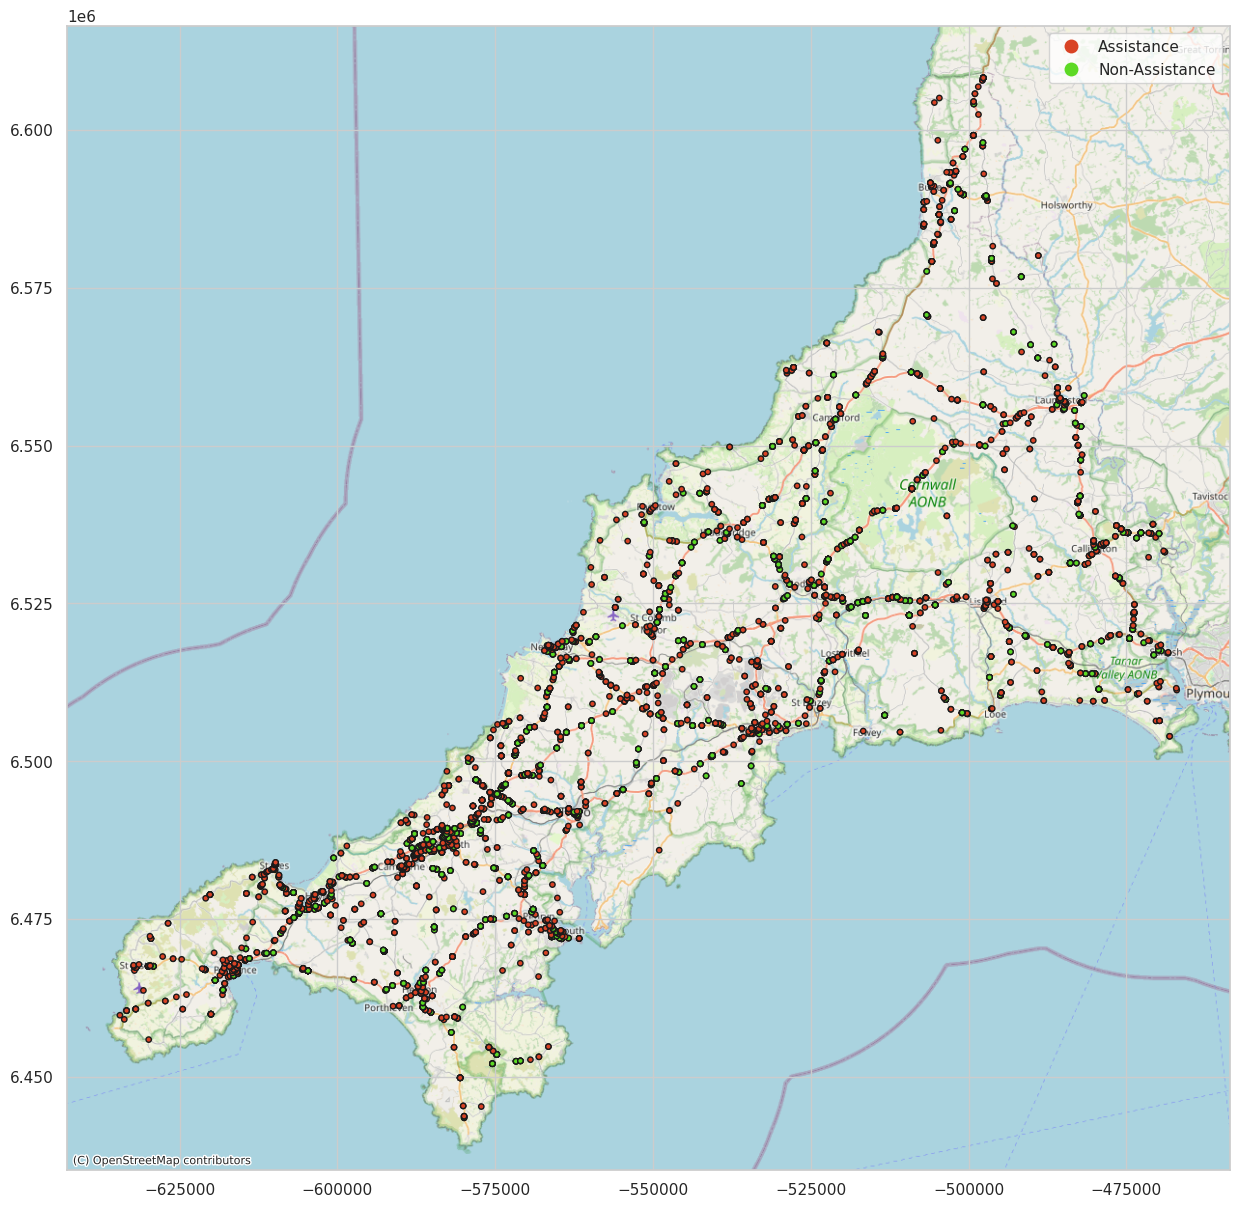
\includegraphics[width=75mm]{Figures/Cornwall/filtered_OpenStreetMap.Mapnik.png}
         \label{CornwallAccidentsMap:Filtered}
     }
     \caption{Cornwall original/filtered accidents map.}
     \label{CornwallAccidentsMap}
 \end{figure}


 \begin{figure}[H]
 \centering
    \subfigure[Training 2D-CNN Southwark]{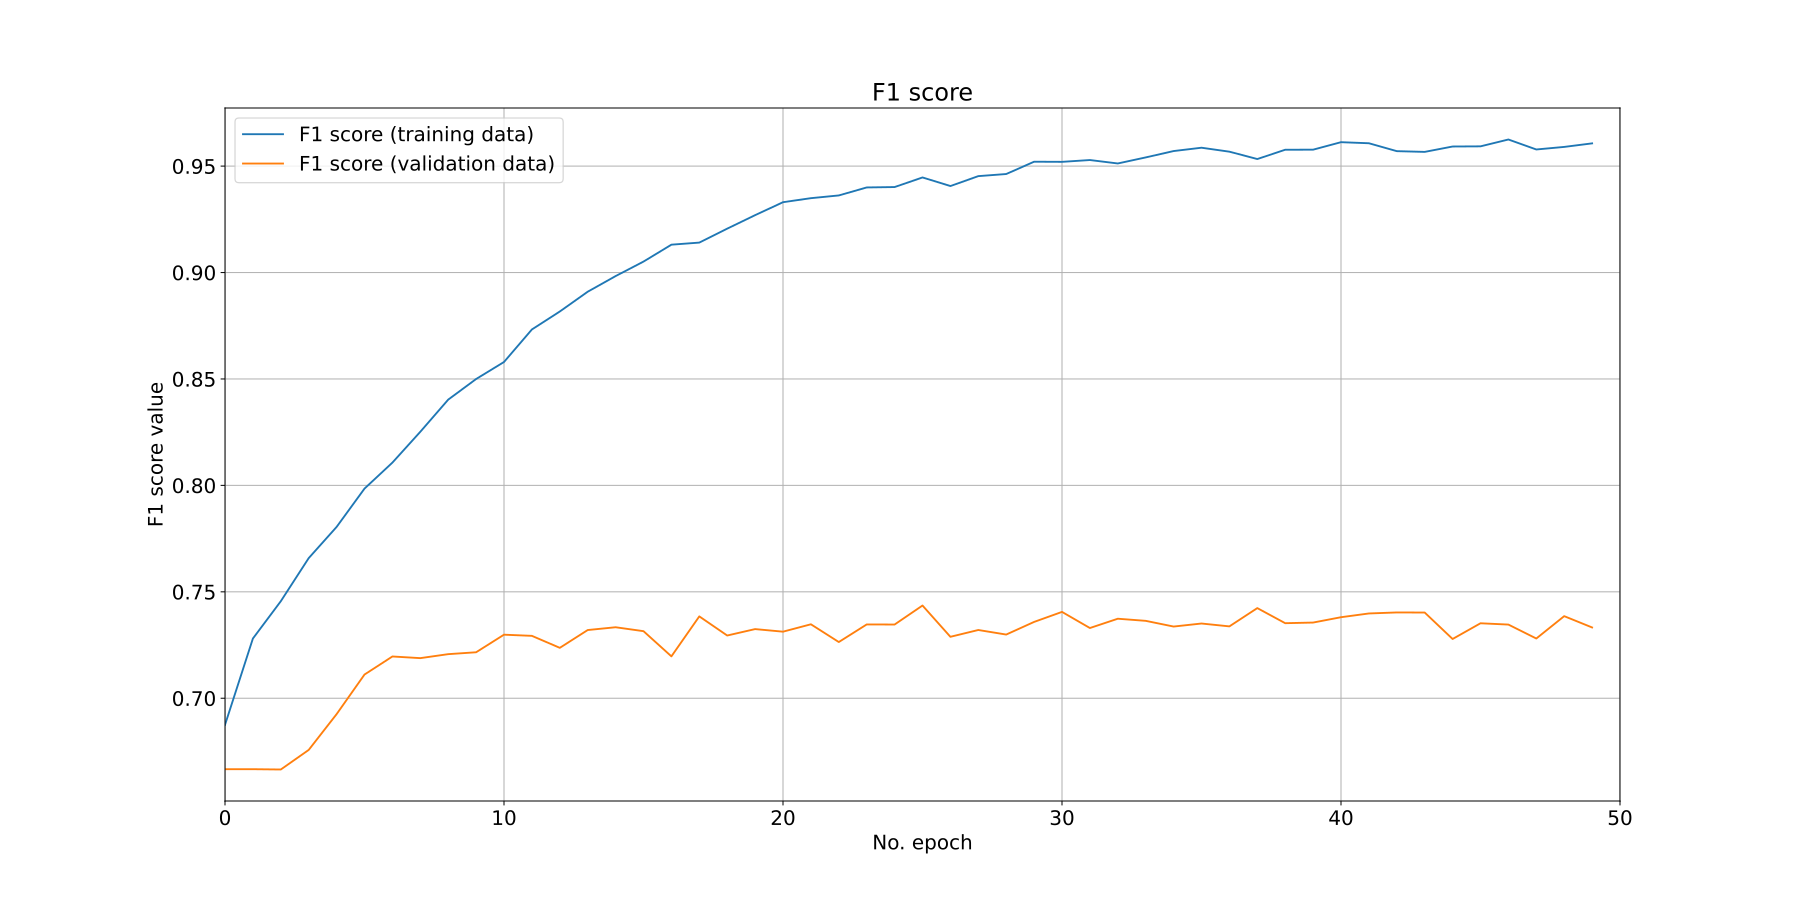
\includegraphics[width=80mm]{Figures/Cornwall/Cornwall_convolution_2d_f1_score_paper.png}}
    \subfigure[Training 2D-CNN Manchester]{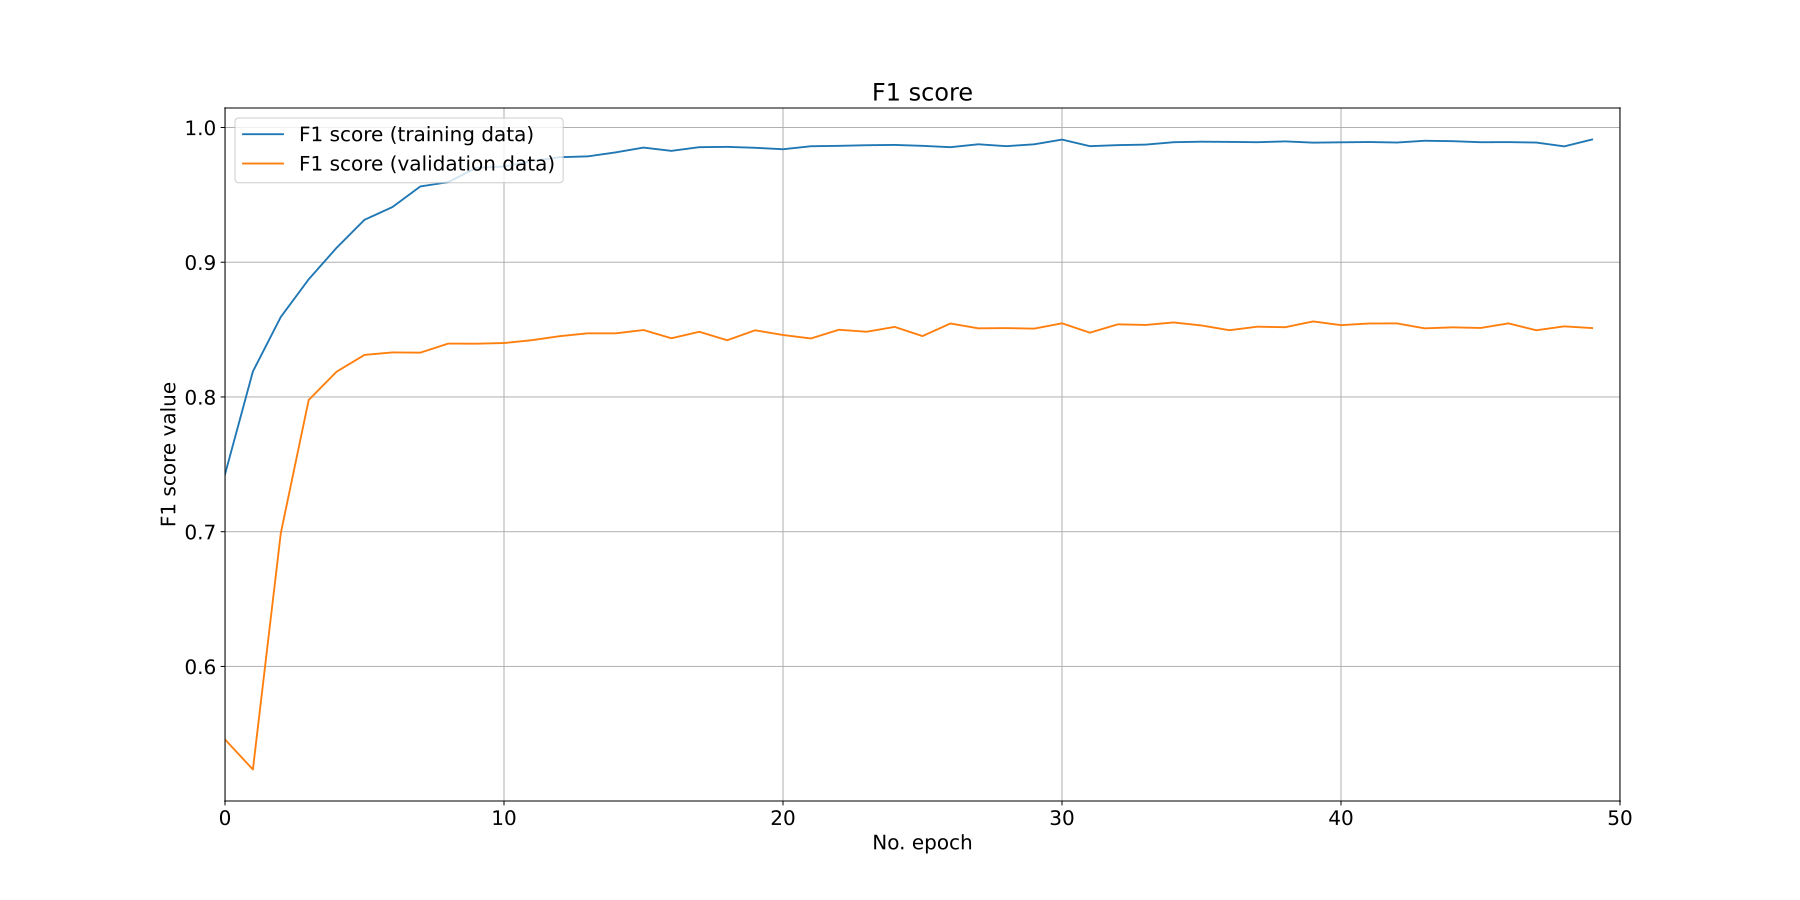
\includegraphics[width=80mm]{Figures/Manchester/Manchester_convolution_2d_f1_score_paper.png}}
    \subfigure[Training 2D-CNN Birmingham]{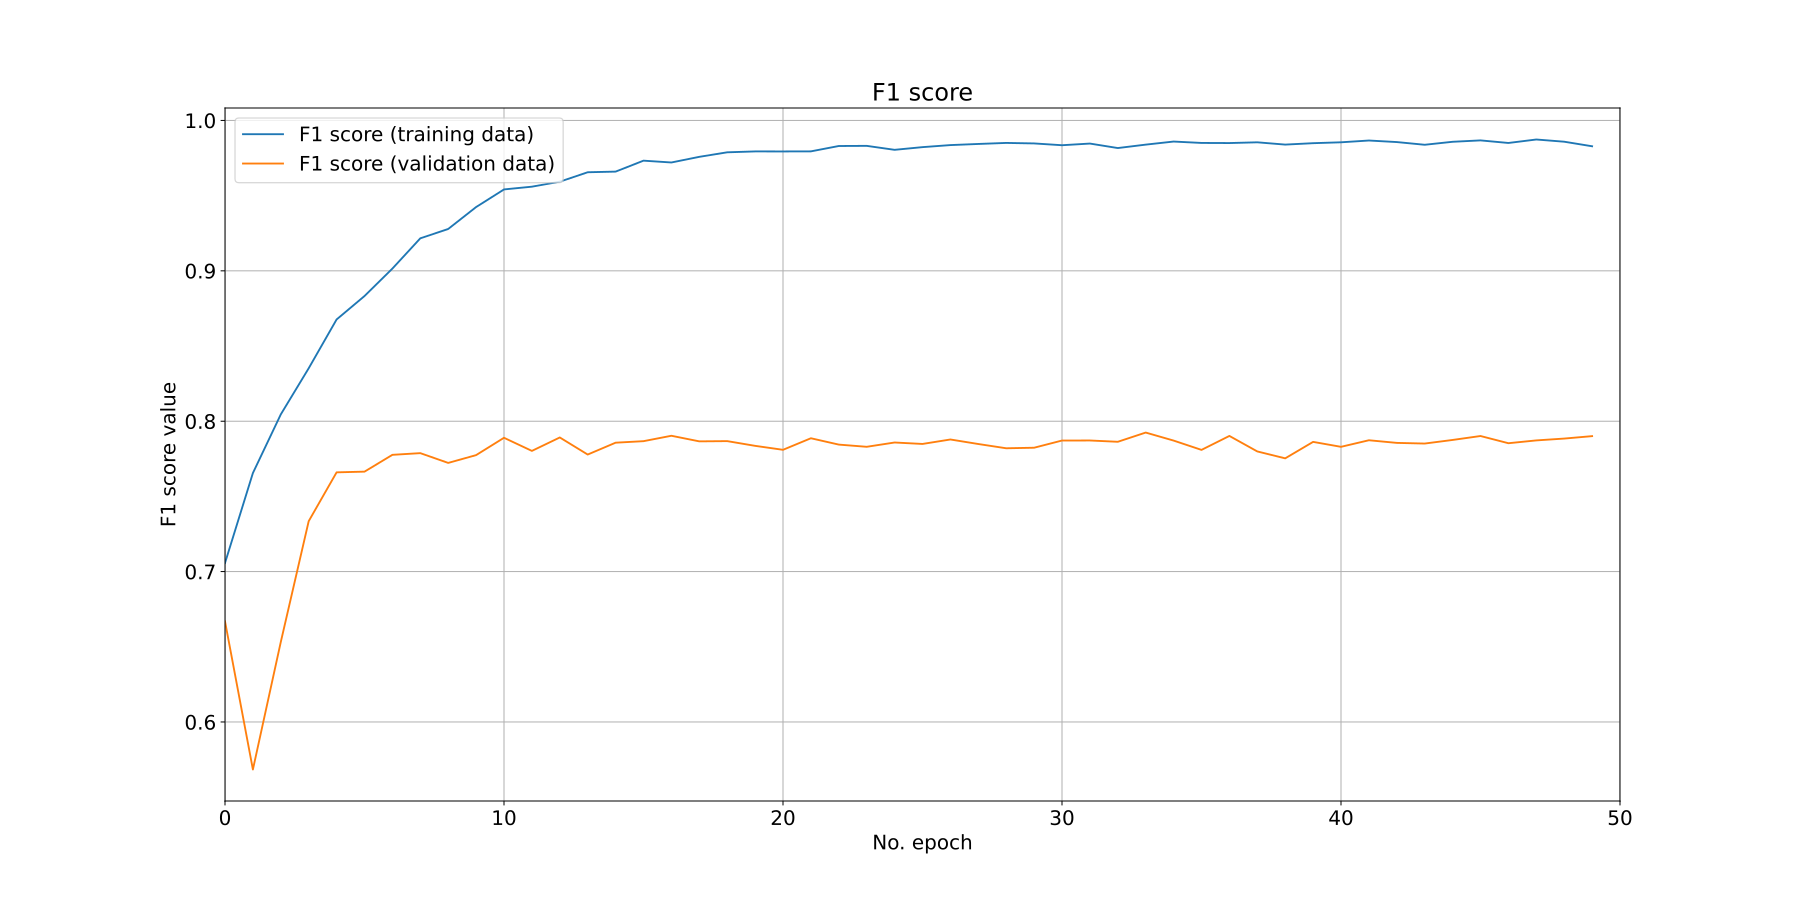
\includegraphics[width=80mm]{Figures/Birmingham/Birmingham_convolution_2d_f1_score_paper.png}}
    \subfigure[Training 2D-CNN Liverpool]{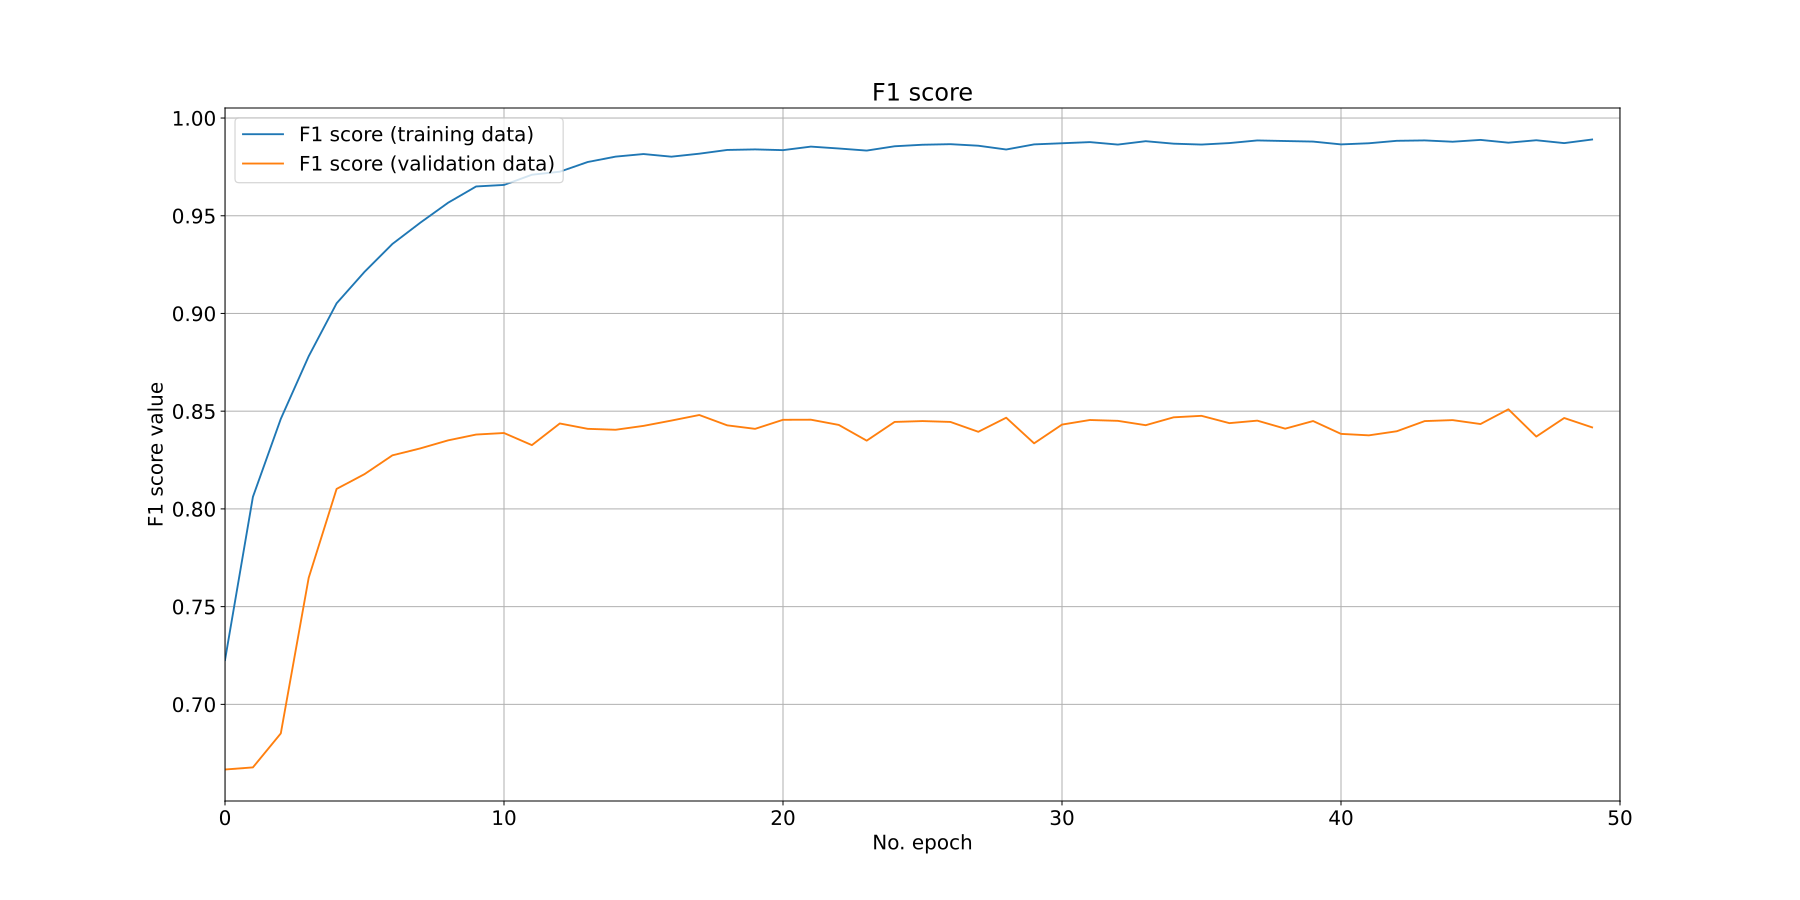
\includegraphics[width=80mm]{Figures/Liverpool/Liverpool_convolution_2d_f1_score_paper.png}}
    \subfigure[Training 2D-CNN Sheffield]{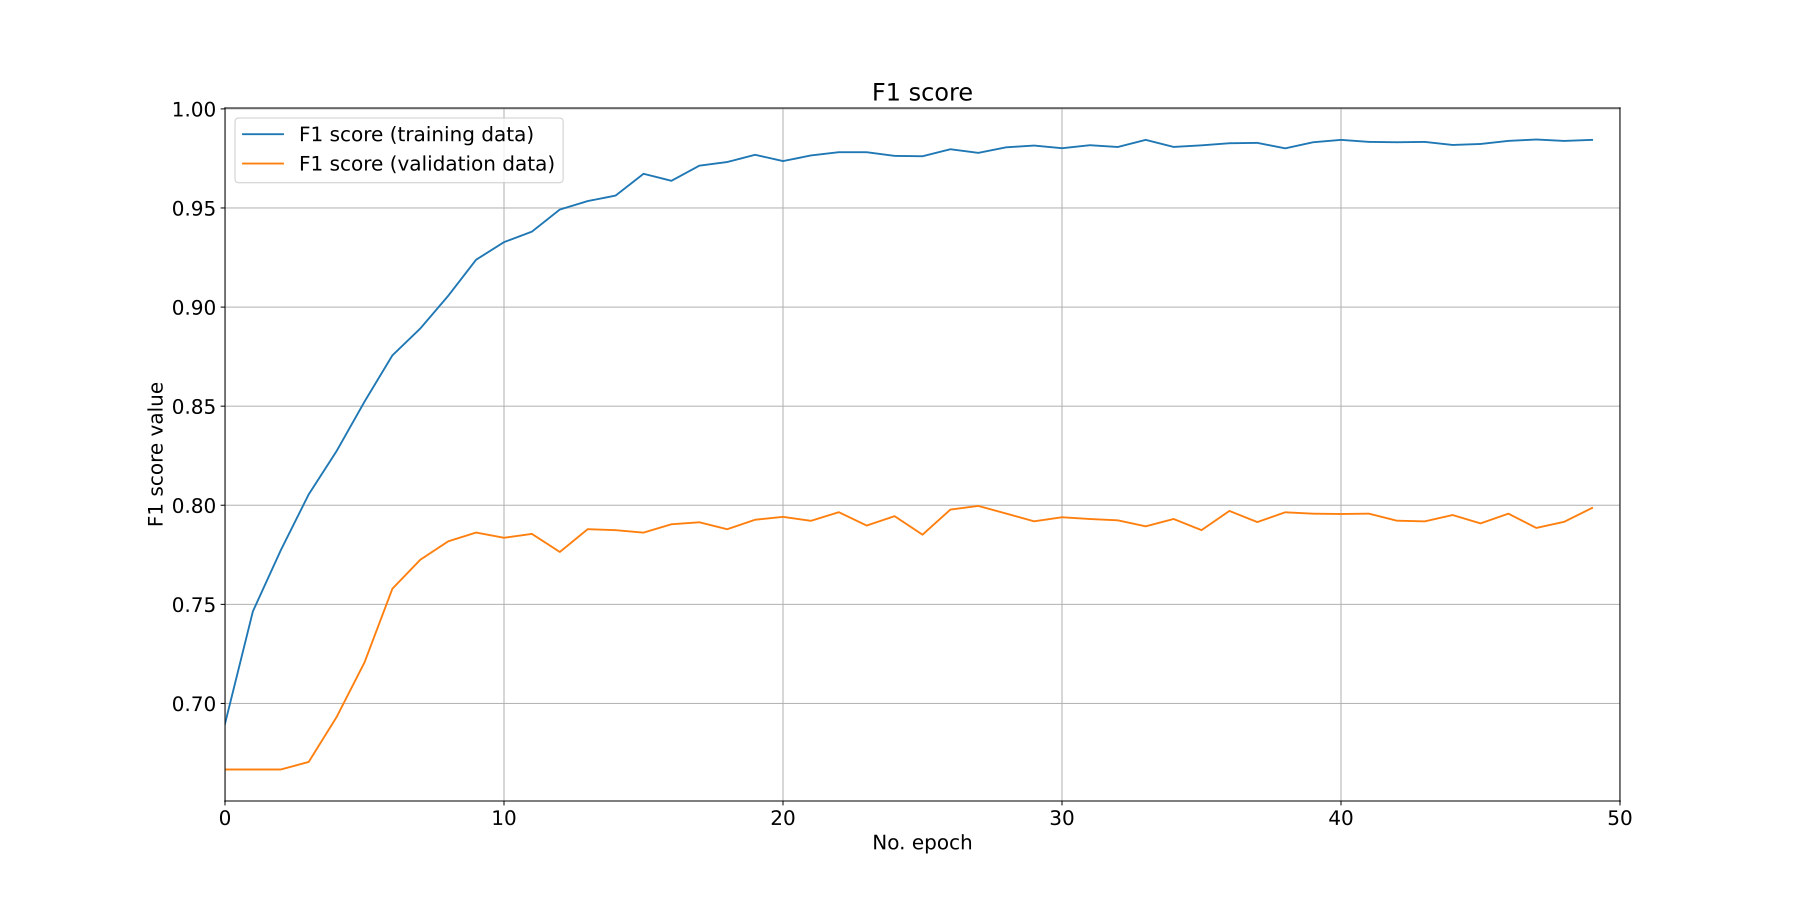
\includegraphics[width=80mm]{Figures/Sheffield/Sheffield_convolution_2d_f1_score_paper.png}}
    \subfigure[Training 2D-CNN Cornwall]{\includegraphics[width=80mm]{Figures/Cornwall/Cornwall_convolution_2d_f1_score_paper.png}}
    \caption{Evolution of F1-Score by UK region.}
 \label{UKLossFunction}
 \end{figure}


En la Tabla \ref{UKMetrics} se muestra el valor F1-Score para cada una de las ciudades de cada modelo sobre el conjunto de test. Como se puede observar, el nuevo modelo propuesto GTAAF es el que mejor métricas ofrece en comparación al resto, obteniendo la mayor diferencia con respecto a su sucesor en los accidentes Slight, el MLP, para la ciudad de Manchester de un 5,33\%, mientras que la mayor diferencia para los accidentes tipo Assitance es de un 13.8\% en la ciudad de Southwark respecto al siguiente mejor modelo, el MLP. La siguiente mayor diferencia se presenta entre el modelo GTAAF se presenta en la ciudad de Southwark para la clase Slight, con un incremento del 4,8\% respecto al siguiente mejor modelo MLP, mientras que para la clase Assistance ésta se presenta en la ciudad de Liverpool con respecto al modelo MLP, llegando a un 13,2\%. Observando los resultados de la tabla, se aprecia que el mayor incremento del rendimiento con respecto al resto de modelos se presenta sobre la clase Assitance, obteniendo de media una mejora de 9,21\% sobre todas las ciudades, mientras que el incremento de rendimiento se acentúa menos en la Slight, ya que el resto de modelos ofrecen unas métricas más altasW, siendo la mejora de un 3,93\% de media. Estos resultados reflejan una mejor generalización del modelo propuesto en comparación al resto de modelos estudiados para cada una de las ciudades de Reino Unido.

\begin{table}[H]
	\begin{center}
		\begin{tabular}{|c|c||c|c|c|c|c|c|}
		\hline
		\multicolumn{2}{ |c|| }{} &
		\multicolumn{6}{ |c| }{\textbf{UK areas F1-Score}} \\ \hline

		\textbf{Model} & \textbf{Assistance} & Southwark & Manchester & Birmingham & Liverpool & Sheffield & Cornwall
		\\ \hline \hline

        \multirow{2}{*}{NB} &
            No & 0.504 & 0.675 &  0.567 & 0.560 & 0.620 & 0.653 \\ &
		    Yes & 0.400 & 0.482 & 0.558 & 0.417 & 0.669 & 0.484 \\ \hline \hline
        \multirow{2}{*}{SVC} &
            No & 0.826 & 0.845 & 0.812 & 0.865 & 0.809 & 0.702 \\ &
		    Yes & 0.599 & 0.624 & 0.673 & 0.630 & 0.773 & 0.626 \\ \hline \hline
        \multirow{2}{*}{KNN} &
            No  & 0.652 & 0.723 & 0.747 & 0.746 & 0.754 & 0.656 \\ &
            Yes & 0.469 & 0.510 & 0.609 & 0.519 & 0.676 & 0.559 \\ \hline \hline
        \multirow{2}{*}{RF} &
            No & 0.561  & 0.118 & 0.303 & 0.742 & 0.313 & 0.711 \\ &
            Yes & 0.430 & 0.379 & 0.509 & 0.504 & 0.585 & 0.581 \\ \hline \hline
        \multirow{2}{*}{LR} &
            No & 0.711 & 0.800 & 0.761 & 0.806 & 0.733 & 0.630 \\ &
            Yes & 0.415 & 0.540 & 0.604 & 0.530 & 0.652 & 0.598 \\ \hline \hline
        \multirow{2}{*}{MLP} &
            No & 0.916 &  0.857 & 0.819 & 0.910 & 0.853 & 0.709 \\ &
            Yes & 0.743 & 0.632 & 0.662 & 0.721 & 0.810 & 0.671 \\ \hline \hline
        \multirow{2}{*}{\textbf     {GTAAF}} &
            \textbf{No} & \textbf{0.964} & \textbf{0.924} & \textbf{0.858} & \textbf{0.956} & \textbf{0.918} & \textbf{0.722} \\ &
            \textbf{Yes} & \textbf{0.881} & \textbf{0.762} & \textbf{0.711} & \textbf{0.853} & \textbf{0.889} & \textbf{0.707} \\ \hline \hline
		\end{tabular}
	\end{center}
	\caption{F1-Scores comparison by traffic accident assistance on six UK areas.}
	\label{UKMetrics}
\end{table}


La Figura \ref{GlobalSlightF1Score} muestra a modo de comparativa el rendimiento del nuevo modelo GTAAF propuesto en los accidentes Slight para cada una de las poblaciones estudiadas respecto al resto de modelos del estado del arte con los que se ha experimentado en esta investigación. Se aprecia un incremento de rendimiento independientemente de las características individuales en todas las poblaciones respecto al resto de modelos estudiados, siendo el mayor incremento en la población de Victoria con un incremento del 6.5\% respecto al siguiente mejor modelo, el SVC.

\begin{figure}[H]
    \centering
    \includegraphics[width=150mm]{Figures/Slight.png}
    \caption{F1-Scores Comparison for Non-Assistance Accidents.}
    \label{GlobalSlightF1Score}
\end{figure}

La Figura \ref{GlobalAssistanceF1Score} muestra la comparativa del rendimiento basado en el F1-Score de los modelos para cada una de las ciudades en los accidentes Assitance. En esta gráfica se puede observar una diferencia cosiderablemente mayor del nuevo modelo GTAAF propuesto respecto al resto en comparación con los accidentes Slight. La mayor diferencia de mejora de este modelo GTAAF se presenta en la ciudad de Southwark, con un incremento del F1-Score del 13.8\% respecto al siguiente mejor modelo sobre esta población, el MLP.

\begin{figure}[H]
    \centering
    \includegraphics[width=150mm]{Figures/Assistance.png}
    \caption{F1-Scores Comparison for Assistance Accidents.}
    \label{GlobalAssistanceF1Score}
\end{figure}

\section{Pruebas de estrés}

En esta sección se realizarán distintas pruebas de estrés. El objetivo de estas pruebas es medir el rendimiento de la metodologúa y el modelo propuesto en casos extremos utilizando como base los conjuntos de datos expuestos en esta tesis para tener una aproximación del rendimiento del modelo en otros conjuntos de datos que no dispongan de las caracteristicas descritas en este documento. Para ello se realizarán tres experimentos para cada conjunto de datos que consistirán en eliminar aquellas características de mayor y menor importancia de forma independiente, y, en un experimento posterior, se eliminarán ambas conjuntamente con el objetivo de medir el rendimiento ante la falta de características más y menos influyentes en futuros conjuntos de datos. La evaluación de la importancia de las características viene dada por el peso asignado a cada una de estas mediante el algoritmo genético.

En la tabla \ref{Madridloss} ...

%%%%%%%%%%%%%%%%%%%%%%%%%%%%%%%%%%%%%%%%%%%%%%%%%%%%%%%%%%%%%%%%%%%%%%%%%%%%%%%%%
\begin{table}[H]
	\begin{center}
		\begin{tabular}{|c|c||c|c|c|c|c|c|}
		\hline
		\multicolumn{2}{ |c|| }{} &
		\multicolumn{3}{ |c| }{\textbf{Cornwall}} \\ \hline

		\textbf{Model} & Assistance & Lowest & Highest & Both
		\\ \hline \hline

        \multirow{2}{*}{NB} &
            No & 0.668 & 0.597 & 0.592\\ &
		    Yes & 0.490 & 0.535 & 0.519 \\ \hline \hline
        \multirow{2}{*}{SVC} &
            No & 0.710 & 0.631 & 0.646\\ &
		    Yes & 0.628 & 0.626 & 0.620 \\ \hline \hline
        \multirow{2}{*}{KNN} &
            No & 0.671 & 0.601 & 0.637\\ &
		    Yes & 0.571 & 0.532 & 0.559 \\ \hline \hline
        \multirow{2}{*}{RF} &
            No & 0.719 & 0.498 & 0.514\\ &
		    Yes & 0.603 & 0.638 & 0.644 \\ \hline \hline
        \multirow{2}{*}{LR} &
            No & 0.670 & 0.575 & 0.567\\ &
		    Yes & 0.626 & 0.585 & 0.580 \\ \hline \hline
        \multirow{2}{*}{MLP} &
            No & 0.724 & 0.652 & 0.680\\ &
		    Yes & 0.695 & 0.654 & 0.685 \\ \hline \hline
        \multirow{2}{*}{\textbf{CNN2D}} &
            No & \textbf{0.768} & \textbf{0.736} & \textbf{0.792}\\ &
		    Yes & \textbf{0.766} & \textbf{0.736} & \textbf{0.787} \\ \hline \hline
		\end{tabular}
	\end{center}
	\caption{\textcolor{red}{F1-Scores comparison with features loss in Madrid dataset. In bold the best result (our model)}}
	\label{Madridloss}
\end{table}
%%%%%%%%%%%%%%%%%%%%%%%%%%%%%%%%%%%%%%%%%%%%%%%%%%%%%%%%%%%%%%%%%%%%%%%%%%%%%%%%%


%%%%%%%%%%%%%%%%%%%%%%%%%%%%%%%%%%%%%%%%%%%%%%%%%%%%%%%%%%%%%%%%%%%%%%%%%%%%%%%%%
\begin{table}[H]
	\begin{center}
		\begin{tabular}{|c|c||c|c|c|c|c|c|}
		\hline
		\multicolumn{2}{ |c|| }{} &
		\multicolumn{3}{ |c| }{\textbf{Victoria}} \\ \hline

		\textbf{Model} & \textbf{Assistance} & Lowest & Highest & Both
		\\ \hline \hline

        \multirow{2}{*}{NB} &
            No & 0.639 & 0.613 & 0.607\\ &
		    Yes & 0.465 & 0.553 & 0.572 \\ \hline \hline
        \multirow{2}{*}{SVC} &
            No & 0.653 & 0.638 & 0.664\\ &
		    Yes & 0.657 & 0.650 & 0.676 \\ \hline \hline
        \multirow{2}{*}{KNN} &
            No & 0.625 & 0.627 & 0.638\\ &
		    Yes & 0.540 & 0.562 & 0.566 \\ \hline \hline
        \multirow{2}{*}{RF} &
            No & 0.630 & 0.630 & 0.621\\ &
		    Yes & 0.248 & 0.161 & 0.071 \\ \hline \hline
        \multirow{2}{*}{LR} &
            No & 0.598 & 0.574 & 0.599\\ &
		    Yes & 0.609 & 0.637 & 0.646 \\ \hline \hline
        \multirow{2}{*}{MLP} &
            No & 0.635 & 0.636 & 0.654\\ &
		    Yes & 0.693 & 0.686 & 0.692 \\ \hline \hline
        \multirow{2}{*}{\textbf{CNN2D}} &
            No & \textbf{0.732} & \textbf{0.720} & \textbf{0.778}\\ &
		    Yes & \textbf{0.780} & \textbf{0.793} & \textbf{0.814} \\ \hline \hline
		\end{tabular}
	\end{center}
	\caption{\textcolor{red}{F1-Scores comparison with features loss in Victoria dataset. In bold the best result (our model)}}
	\label{Victorialoss}
\end{table}
%%%%%%%%%%%%%%%%%%%%%%%%%%%%%%%%%%%%%%%%%%%%%%%%%%%%%%%%%%%%%%%%%%%%%%%%%%%%%%%%%

En este experimento es necesario destacar un resultado: en nuestra propuesta, el modelo GTAAF, existe una gran mejora sobre los resultados del mismo modelo con todas las características. En contraste, hay un gran deterioro en los resultados de los otros modelos con los que se compara. En otras palabras, la diferencia en el puntaje F1 entre GTAAF y los otros modelos aumenta.

Esta circunstancia sugiere que nuestro modelo se ve afectado por las características extremas, donde el modelo de boosting y el algoritmo genético favorecen y desfavorecen las características más y menos relevantes. Este no es el caso para los otros algoritmos, donde todas las características son individualizadas.

En la Figura \ref{lossFig} podemos observar la diferencia de los algoritmos con y sin pérdida de características (Tablas \ref{UKMetrics} y \ref{AustraliaMetrics} versus Tablas \ref{CornwallLoss} y \ref{Victorialoss}). Mostramos cómo nuestro modelo mejora sus propios resultados en todos los casos.

Por ejemplo, en Cornwall, obtenemos una mejora en nuestro modelo del 4.8\% y 5.9\% en No Assistance y Assistance (eliminando la peor característica, ver la barra azul en la Figura \ref{lossFig}-arriba), 1.4\% y 2.9\% (eliminando la mejor característica, ver la barra verde en la Figura \ref{lossFig}-arriba) y 7\% y 8\% (eliminando ambas características, ver la barra gris en la Figura \ref{lossFig}-arriba), respectivamente.

Evaluando un área más dispersa como Victoria, los resultados son similares pero con una mejora menor: 0.5\% y 0.4\% (ver la barra azul en la Figura \ref{lossFig}-abajo), -0.7\% y 0.9\% (ver la barra verde en la Figura \ref{lossFig}-abajo), y 5.1\% y 3\% (ver la barra gris en la Figura \ref{lossFig}-abajo), respectivamente. Esto indicaría un efecto menor de los valores extremos en la ponderación del algoritmo genético si el área es más dispersa.

\begin{figure}[H]
	\centering
	\includegraphics[width=180mm]{Figures/LossFeatures/loss.png}
	\caption{Comparación de pérdida de características. Las barras representan la diferencia entre los resultados con todas las características y los resultados sin características extremas: en azul sin la característica más baja, en verde sin la característica más alta y en gris sin ambas características extremas.}
	\label{lossFig}
\end{figure}


\chapter{Conclusiones}


En esta tesis se ha propuesto un nuevo modelo que evalúa la necesidad de asistencia médica en los accidentes de tráfico. Esta funcionalidad es extremadamente importante para priorizar la asignación de recursos médicos una vez se conocen las caracteristicas del accidente, de tal forma que se puedan minimizar las consecuencias físicas a corto y largo plazo de las víctimas. Para ello se ha propuesto una metodología que transforma las características que describen los accidentes, mediante categorizaciones, para alimentar a nuestro modelo convolucional X. Como se ha demostrado en su evaluación, los resultados no solo mejoran ampliamente al estado del arte (con valores de hasta el 13.8\%), sino que la categorización propuesta ha demostrado ser muy robusta respecto a la individualización de características de los demás modelos. Además, nuestro modelo ha mostrado un gran rendimiento en distintos contextos, concretamente en  distintos datasets de 8 poblaciones de diferentes densidades de población, siendo relevante este dato en la correlación que tiene con el número de accidentes producidos.\\

Además, con el objetivo de proponer un modelo general que pueda ser aplicado a nuevas poblaciones que no dispongan de la misma información que los datasets presentados en este artículo, (debido principalmente a la dificultad inherente de recogida de datos específicos, como controles de alcohol y drogas, u otras características cuya obtención esté relacionada con la condición económica de la población), se ha analizado la robustez del modelo eliminando características, excluyendo características de mayor y menor impacto que han resultado del algoritmo genético, obteniendo resultados incluso mejores en nuestro modelo que hace indicar la sensibilidad que tiene éste respecto a estos valores. Como trabajo futuro se analizará cómo reducir esta sensibilidad.

\chapter{Publications}






\chapter{Anexos}

Madrid paper I discretization:
\begin{table}[H]
\begin{center}
\renewcommand{\arraystretch}{1.4}
\scriptsize
\begin{minipage}{0.4\textwidth}
\begin{tabular}{|l|l|}
    \hline
    \textbf{Features} & \textbf{Typing}\\
    \hline
    \multirow{\textbf{Severity}}  & 0: Slight (\textit{1, 2, 5, 6, 7})\\
                                & 1: Severe (\textit{3})\\
                                & 2: Fatal (\textit{4})\\
    \hline
    \multirow{Time}     & 1: Night (\textit{6 PM - 6 AM})\\
                        & 2: Day (\textit{6 AM - 6 PM})\\
    \hline
    \multirow{District}   & Based on order of appearance\\
    \hline
    \multirow{X}   & UTM X Coordinate position\\
    \hline
    \multirow{Y}   & UTM Y Coordinate position\\
    \hline
    \multirow{Type of Accident} & 1: Head-on - size collision \\
                                & 2: Rear-end collision\\
                                & 3: Side crash\\
                                & 4: Collision again fixed obstacle\\
                                & 5: Pile-up\\
                                & 6: Hitting a pedestrian\\
                                & 7: Head-on collision\\
                                & 8: Other\\
                                & 9: Leaving the road\\
                                & 10: Vehicle rollover\\
                                & 11: Hitting an animal\\
                                & 12: Falling\\
    \hline
    \multirow{Type of Road}     & 1: Parking \\
                                & 2: Airport\\
                                & 3: Park\\
                                & 4: Tunnel\\
                                & 5: Industrial state\\
                                & 6: Track\\
                                & 7: Round\\
                                & 8: Roundabout\\
                                & 9: Gate\\
    \hline
    \end{tabular}
    \end{minipage} \hspace{10mm}
    \begin{minipage}{0.4\textwidth}
    \begin{tabular}{|l|l|}
    \hline
    \textbf{Feature} & \textbf{Typing}\\
    \hline
    \multirow{Type of Road}     
                                & 10: Bridge\\
                                & 11: Square\\
                                & 12: Boulevard\\
                                & 13: Crossing\\
                                & 14: Roadway\\
                                & 15: Road\\
                                & 16: Avenue\\
                                & 17: Highway\\
                                & 18: Street\\
    \hline
    \multirow{Weather Conditions}   & 1: Sunny\\
                                    & 2: Cloudy\\
                                    & 3: Light rain\\
                                    & 4: Heavy rain\\
                                    & 5: Hail\\
                                    & 6: Snowing\\
                                    & 7: Unknown\\
    \hline
    \multirow{Vehicle}  & Based on order of appearance\\
    \hline
    \multirow{Person}   & 1: Driver\\
                        & 2: Passenger\\
                        & 3: Pedestrian\\
    \hline
    \multirow{Age}      & 1: Under 18 years of age\\
                        & 2: From 18 to 25 years old\\
                        & 3: From 25 to 65 years old\\
                        & 4: Over 65 years old\\
                        & 5: Unknown\\
    \hline
    \multirow{Gender}   & 1: Male\\
                        & 2: Female\\
                        & 3: Unknown\\
    \hline
    \multirow{Alcohol or Drugs} & 1: Yes\\
                                & 2: Not\\
    \hline
\end{tabular}
\end{minipage}
\end{center}
\caption{Numerical assignment of the dataset variables.}
\label{TransformacionDatosTabla}
\end{table} 

% ----------------------------------------------
% Bibliografía
% ----------------------------------------------

\bibliography{bibliography}






\bibliographystyle{plain}

\end{document}
